% !TeX root = main_submission.tex

\documentclass[superscriptaddress,
               floatfix,
               longbibliography, 
               showkeys,apl]{revtex4-2}  
  
%\bibliographystyle{apsrevtitle}

\usepackage{graphicx} 
\usepackage{bm}	
\usepackage{color}                     
\usepackage{xcolor}
\usepackage{epsfig}
\usepackage{amsmath} 
\usepackage{amssymb} 
\usepackage{longtable} 
\usepackage{float}
\usepackage{mathtools}
\usepackage{dsfont}
\usepackage{xparse}
\usepackage{hyperref}
\usepackage{times}
\usepackage[normalem]{ulem}
\usepackage{sidecap}
\usepackage{appendix} 
\sidecaptionvpos{figure}{t}
\usepackage{comment}
\usepackage{physics}
\usepackage{float}
\usepackage{xfrac}
\newtheorem{theorem}{Theorem}
\usepackage{svg}
\usepackage{multirow}

%% Text flags
\definecolor{darkgreen}{rgb}{0.0, 0.5, 0.0}
\newcommand{\wip}[2]{\textcolor{darkgreen}{[#1] #2}}

%\newcommand{\eg}{e.g.}
%\newcommand{\ie}{i.e.}

%PQC tasks
\newcommand{\ansatz}{\mathcal{U}} % Ansatz
\newcommand{\pqc}{\ansatz(\params)} % PQC

\newcommand{\objective}{C} % cost operator
\newcommand{\objectiveparams}{\objective(\params)} % cost operator

\newcommand{\costfunction}{\mathcal{C}} % PQC
\newcommand{\costfunctionstate}{\costfunction(\psi)} % PQC
\newcommand{\costoperator}{\mathcal{O}} % cost operator

\newcommand{\taskidx}{\tau} % cost operator
\newcommand{\taskidxtest}{\tau^{\prime}} % cost operator
\newcommand{\stateinit}{|\psi_0 \rangle} % cost operator
\newcommand{\statefinal}{|\psi(\params) \rangle}
\newcommand{\state}{|\psi \rangle}

\newcommand{\proj}[1]{|#1\rangle \langle #1|}


\newcommand{\be}{\begin{equation}}
\newcommand{\ee}{\end{equation}}
\newcommand{\bd}{\begin{displaymath}}
\newcommand{\ed}{\end{displaymath}}
\newcommand{\BE}{\begin{eqnarray}}
\newcommand{\EE}{\end{eqnarray}}
\newcommand{\vsp}{\vspace*{3mm}}
\newcommand{\pprime}{{\prime\prime}}
\newcommand{\R}{{\rm I\!R}}
\newcommand{\smallo}{{o}}
\newcommand{\plus}{{\!+\!}}
\newcommand{\minus}{{\!-\!}}
\newcommand{\sgn}{{\rm sgn}}
\newcommand{\erfc}{{\rm erfc}}
\newcommand{\id}{{\rm 1\!\!I}}
\newcommand{\ba}{\ensuremath{\mathbf{a}}}
\newcommand{\bb}{\ensuremath{\mathbf{b}}}
\newcommand{\bc}{\ensuremath{\mathbf{c}}}
\newcommand{\bh}{\ensuremath{\mathbf{h}}}
\newcommand{\bk}{\ensuremath{\mathbf{k}}}
\newcommand{\bq}{\ensuremath{\mathbf{q}}}
\newcommand{\bs}{\ensuremath{\mathbf{s}}}
\newcommand{\bu}{\ensuremath{\mathbf{u}}}
\newcommand{\bv}{\ensuremath{\mathbf{v}}}
\newcommand{\bw}{\ensuremath{\mathbf{w}}}
\newcommand{\bx}{\ensuremath{\mathbf{x}}}
\newcommand{\by}{\ensuremath{\mathbf{y}}}
\newcommand{\bz}{\ensuremath{\mathbf{z}}}
\newcommand{\bn}{\ensuremath{\mathbf{n}}}
\newcommand{\bolde}{\ensuremath{\mathbf{e}}}
\newcommand{\bee}{\ensuremath{\mathbf{e}}}
\newcommand{\boldeff}{\ensuremath{\mathbf{f}}}
\newcommand{\bA}{\ensuremath{\mathbf{A}}}
\newcommand{\bB}{\ensuremath{\mathbf{B}}}
\newcommand{\bC}{\ensuremath{\mathbf{C}}}
\newcommand{\bD}{\ensuremath{\mathbf{D}}}
\newcommand{\bF}{\ensuremath{\mathbf{F}}}
\newcommand{\bG}{\ensuremath{\mathbf{G}}}
\newcommand{\bGz}{\ensuremath{\mathbf{G_0}}}
\newcommand{\bRone}{\ensuremath{\mathbf{R_1}}}
\newcommand{\bJ}{\ensuremath{\mathbf{J}}}
\newcommand{\bK}{\ensuremath{\mathbf{K}}}
\newcommand{\bR}{\ensuremath{\mathbf{R}}}
\newcommand{\bT}{\ensuremath{\mathbf{T}}}
\newcommand{\bW}{\ensuremath{\mathbf{W}}}
\newcommand{\bM}{\ensuremath{\mathbf{M}}}
\newcommand{\bp}{\ensuremath{\mathbf{p}}}
\newcommand{\bCx}{\ensuremath{\mathbf{C_1}}}
\newcommand{\bCy}{\ensuremath{\mathbf{C_2}}}
\newcommand{\bGx}{\ensuremath{\mathbf{G_1}}}
\newcommand{\bGy}{\ensuremath{\mathbf{G_2}}}
\newcommand{\beff}{\ensuremath{\mathbf{f}}}
\newcommand{\hq}{\hat{q}}
\newcommand{\hw}{\hat{w}}
\newcommand{\hx}{\hat{x}}
\newcommand{\hy}{\hat{y}}
\newcommand{\hA}{\hat{A}}
\newcommand{\hC}{\hat{C}}
\newcommand{\hG}{\hat{G}}
\newcommand{\hK}{\hat{K}}
\newcommand{\hL}{\hat{L}}
\newcommand{\D}{{\cal{D}}}
\newcommand{\hbq}{\hat{\mbox{\boldmath{q}}}}
\newcommand{\qbo}{{\mbox{\boldmath{q}}}}
\newcommand{\hbx}{\hat{\mbox{\boldmath{x}}}}
\newcommand{\hbw}{\hat{\mbox{\boldmath{w}}}}
\newcommand{\hOmega}{\hat{\mbox{$\Omega$}}}
\newcommand{\bchi}{{\mbox{\boldmath{$\chi$}}}}
\newcommand{\boldeta}{{\mbox{\boldmath{$\eta$}}}}
\newcommand{\boldomega}{{\mbox{\boldmath{$\omega$}}}}
\newcommand{\boldpsi}{{\mbox{\boldmath{$\psi$}}}}
\newcommand{\boldphi}{{\mbox{\boldmath{$\varphi$}}}}
\newcommand{\bEta}{{\mbox{\boldmath{$\eta$}}}}
\newcommand{\bzeta}{{\mbox{\boldmath{$\zeta$}}}}
\newcommand{\boldOmega}{{\mbox{\boldmath{$\Omega$}}}}
\newcommand{\bxi}{\bm{\xi}}
\newcommand{\olx}{\overline{\mathbf{x}}}
\newcommand{\olxone}{\overline{x}_1}
\newcommand{\olxtwo}{\overline{x}_2}
\newcommand{\olxonedot}{\dot{\overline{x}}_1}
\newcommand{\olxtwodot}{\dot{\overline{x}}_2}
\newcommand{\bnull}{{\mbox{\boldmath{$0$}}}}
\newcommand{\rate}{\tilde{\eta}}
\newcommand{\double}{{\prime\prime}}
\newcommand{\tp}{t^\prime}
\newcommand{\td}{t^{\prime\prime}}
\newcommand{\wt}{\widetilde}
\newcommand{\avg}[1]{\left\langle{#1}\right\rangle}
\newcommand{\davg}[1]{\left\langle\left\langle{#1}\right\rangle\right\rangle}
\newcommand{\fE}{\mathbb{E}}
\newcommand{\ds}{\mathcal{D}\,\mathbf{S}}
\newcommand{\mcD}{\mathcal{D}}
\newcommand{\mcM}{\mathcal{M}}

\newcommand{\Jferro}{J_{\mathrm{F}}}


\newcommand{\Ham}[1]{H_{\mathrm{#1}}}
\newcommand{\Hnumfault}{\Ham{numfaults}}
\newcommand{\Hgate}{\Ham{gate}}
\newcommand{\Hfaultset}{\Ham{faultset}}
\newcommand{\Hconsist}{\Ham{consist}}
\newcommand{\Hmultfault}{\Ham{multfault}}
\newcommand{\weight}[1]{\lambda_{\mathrm{#1}}}
\newcommand{\faultweight}{\weight{faultset}}
\newcommand{\multfaultweight}{\weight{multfault}}
\newcommand{\gateweight}{\weight{gate}}
\newcommand{\OR}{\textsc{OR}}
\newcommand{\AND}{\textsc{AND}}
\newcommand{\XOR}{\textsc{XOR}}
\newcommand{\EQ}{\textsc{EQ}}
\newcommand{\BUFFER}{\textsc{BUFFER}}
\newcommand{\NOR}{\textsc{NOR}}
\newcommand{\NOT}{\textsc{NOT}}
\newcommand{\NAND}{\textsc{NAND}}

\renewcommand{\labelenumi}{(\roman{enumi})}
\newcommand{\expectedval}[1]{{\mathbb E}\left[ #1 \right]}
\newcommand{\probability}[1]{{\mathbb P}\left[ #1 \right]}


\DeclareMathOperator{\sign}{sign}
\DeclareMathOperator*{\argmin}{arg\,min}

\providecommand{\abs}[1]{\lvert#1\rvert}

\def\c#1{\textcolor{blue}{#1}}
\def\cc#1{\textcolor{red}{#1}}
\def\ccc#1{\textcolor{green}{#1}}

\newcommand{\fs}[1]{\textcolor{blue}{#1}}
\def\hs#1{\textcolor{magenta}{[#1]}}
\newcommand{\ws}[1]{\textcolor{orange}{#1}}
\newcommand{\pjl}[1]{\textcolor{darkgreen}{#1}}
\def\aak#1{\textcolor{orange}{[#1]}}
\def\apo#1{\textcolor{cyan}{#1}}
\def\apoNote#1{\textcolor{cyan}{\textbf{ [#1]} }}

\def\mm#1{\textcolor{green!10!orange!90!}{#1}}


%\NewDocumentCommand{\ceil}{s O{} m}{
%  \IfBooleanTF{#1} 
%    {\left\lceil#3\right\rceil} 
%    {#2\lceil#3#2\rceil} 
%}

\hyphenation{OptDigits}

\begin{document}


\title{Sparse Block-Encodings for Linear Combinations of Ladder Operators}


\date{\today} 

\ws{You can make comments}
\gus{using your shortcut}
\ks{and it'll put}
\ar{your comments}
\pjl{in your own color :D}

\begin{abstract}
\label{abstract}

In this work, we detail the construction of block-encodings for observables described as a linear combination of products of ladder operators acting on fermionic, antifermionic, and bosonic modes.
We refer to this constuction as LOBE (Ladder Operator Block-Encoding) and show how it can be used to simulate Hamiltonians involving interactions between these different types of particles.
Our work builds off of similar sparse block-encoding constructions for fermionic system, but generalizes them to include bosonic ladder operators.
Additionally, we establish a clear connection between these sparse block-encodings and LCU (Linear Combination of Unitaries) block-encodings.
This connection allows for implementations of these block-encodings that significantly reduce the rescaling factor of the block-encoding without significantly affecting the quantum resources required to implement the block-encoding.
Constructing efficient block-encodings that allow for interactions between fermions, antifermions, and bosons, paves the way for the simulation of systems that are not purely fermionic which is vital for the simulation of many models arise in high-energy physics.

\end{abstract} 

\maketitle

\section{Introduction}
\label{sec:intro}

The simulation of many-body quantum systems is a promising potential application for quantum computers \cite{feynman2018simulating}.
Accessing the information of non-unitary operators - such as the Hamiltonian - within a quantum algorithm, which is comprised solely of unitary operations, is a necessary subroutine for performing such simulations.
This task has been pursued through various means, resulting in methods such as Trotterization \cite{suzuki1976generalized,hatano2005finding,lie1893theorie,trotter1959product,childs2021theory} and Block-Encoding \cite{lin2022lecture, poulin2018quantum, low2019hamiltonian}.

Block-Encoding describes a general strategy for encoding a non-unitary operator within a chosen subspace (block) of a larger unitary operator.
Two general frameworks for constructing block-encodings of different operators - sparse block-encodings \cite{berry2009black, childs2009universal, lin2022lecture} and Linear Combinations of Unitaries (LCU) \cite{childs2012hamiltonian} - have allowed for the exploration of explicitly compiled block-encodings of several systems.

Understanding the spacetime quantum resources - the number of qubits (space), the number of operations (time), and the rescaling factor (overhead) - required for quantum simulation algorithms is important for understanding the feasability of simulating different systems.
These quantum resource estimates are crucial as they allow us to gauge the practical usefulness of quantum computers, particularly those that have experimentally demonstrated quantum error correction \cite{bluvstein2024logical, acharya2024quantum}.

Many previous works have investigated the quantum simulation for purely fermionic systems, with a particular emphasis on the simulation of molecules in quantum chemistry \cite{aspuru2005simulated, peruzzo2014variational, babbush2014adiabatic, o2016scalable, babbush2018encoding, google2020hartree, lee2021even, kivlichan2020improved, campbell2021early}.
Another interesting set of quantum systems to simulate are those that are derived from quantum field theories \cite{Peskin:1995ev, jordan2012quantum} \ws{@Gus, pls add citation for all models (quartic, static, phi, yukawa)}, which have applications in areas such as high-energy physics \cite{bauer2023quantum}.
These systems often include interactions between fermions, antifermions, and bosons and several works have produced quantum resource estimates for simulating such systems \cite{camps2024explicit, liu2024efficient, rhodes2024exponential}.

In this work, we provide a novel framework for constructing block-encodings of second-quantized operators, which we refer to as Ladder-Operator Block-Encoding (LOBE).
This framework directly block-encodes operators comprised of creation and annihilation operators and does not require the use of operator transformations that expand fermionic \cite{jordan1928paulische, bravyi2002fermionic, seeley2012bravyi} and bosonic \cite{somma2005quantum} \ws{add standard binary citations} ladder operators in the Pauli operator basis.

We give numerical quantum resource estimates for implementing block-encodings of several classes of operators and several Hamiltonians that arise in quantum field theories.
This includes purely fermionic systems, purely bosonic systems, and systems which include fermions, antifermions, and bosons. 
We analyze the numerical spacetime quantum resources for LOBE - in comparison to techniques which require mapping ladder operators onto the Pauli basis - and find that LOBE results in constructions with better asymptotic scaling and lower numerical quantum resources for many of the systems examined.

This work is organized as follows.
In Section \ref{sec:theory}, we review the defined action of ladder operators on quantum states.
In Section \ref{sec:block-encoding}, we review block-encodings and discuss frameworks for constructing block-encodings of different operators.
In Section \ref{sec:ladder-op-oracles}, we describe the LOBE framework, show compiled block-encodings for several classes of second-quantized operators, and give analytical spacetime costs of the associated constructions.
In Section \ref{sec:results}, we provide numerical quantum resource estimates for block-encodings of various classes of operators and Hamiltonians.
In Section \ref{sec:conclusions}, we summarize the results presented in this work and discuss future directions.
Additionally, a glossary that defines the terminology and variables used throughout this work is given in Appendix \ref{sec:glossary}.

\section{Theory}

%Give background of ladder operators and constructions of realistic Hamiltonians/Observables from ladder Operators
In quantum field theories and quantum chemistry, the main method of keeping track of multiparticle states is known as second quantization \cite{Sakurai_Napolitano_2020}.
In second quantization, multiparticle state vectors are written as $\ket{n} = \ket{n_{I-1}, \dots, n_1, n_0}$ where $n_i \in \mathbb{Z}$ is the number of particles present in mode $i$.
The fermionic (and antifermionic) occupancy of a mode can either be $0$ or $1$ due to the Pauli exclusion principle \gus{cite PEP}.

There is no physical limitation on the occupancy of bosonic modes: $n_{i_a} \in [0, 1, 2, \dots)$.
This leads to an infinitely large space, therefore we can impose an artificial occupancy cutoff ($\Omega$) such that $n_{i_a} \in [0, 1, 2, \Omega)$ and the space becomes finite.
The cutoff on the occupancy can introduce error as some physically allowable states become inaccessible.
However, $\Omega$ can often be chosen such that this error is either zero (if high-occupancy states are never accessed) or reasonable small and the contribution of the magnitude of the error is known. 
\ws{@Kamil/@Gus, is this a fair statement? Is there something we can cite for either no-error or known-error cases?}

The space spanned by the second-quantized state vectors is called the \textit{Fock space} ($\mathcal{F}$) and the state vectors are referred to as \textit{Fock states}.
In second quantization, the Hilbert space is promoted to the Fock space via \cite{Schwartz_2013}:
\begin{equation}
    \mathcal{F} = \oplus_n \mathcal{H}_n.
\end{equation}

Second quantization appears in quantum chemistry after projecting the Hamiltonian onto basis wavefunctions, and ensuring exchange symmetry via Slater determinants. \gus{Will, you know more about quantum chemistry than me, so please edit this as needed}.
Similarly, in quantum field theories, field operators, rather than wavefunctions, are the main objects of the theory. These field operators act on second-quantized states to create and annihilate particles in the field. 

In second quantization, creation and annihilation operators - which will collectively be refered to as \emph{ladder operators} - are used to manipulate the state of the system.
Creation operators increase the occupancy of the mode they act on, while annihilation operators decrease the occupancy.
Many observables (such as Hamiltonians) can be efficiently expressed as products and/or sums of ladder operators.  

Field operators \ws{@Gus, what is a field operator?} in quantum field theories are written in terms of ladder operators as
\begin{equation}
    \phi(x) = \int \frac{d^3p}{(2\pi)^3}\frac{1}{\sqrt{2E_p}}\left(a_p e^{ipx} + a_p^\dagger e^{-ipx}\right).
\end{equation}
\ws{Make sure every variable in an equation is defined either before or after. So here we need to say what $\phi$, $p$, $E_p$, $a_p$, and $x$ are.}
The Hamiltonian can then be derived from the field operators via 
\begin{equation}
    H = \int d^3x \left(\frac{\partial \mathcal{L}}{\partial \dot{\phi}}\dot{\phi} - \mathcal{L} \right)
\end{equation}

Quantum field theory Hamiltonians derived in this way are constructed in terms of products of ladder operators acting on \emph{different types} of particles.

\subsection{Ladder Operators}
\label{subsec:operators}

%\ws{@Gus, you probably have much better language to define all of this stuff. I just needed to write something down so I could reference it in the circuit construction. Don't hesitate to scrap anything in here.}
\subsubsection{Feromons and Antiferomons}

%Define action of fermionic ladder operators.

Fermions (and antifermions) obey the Pauli-exclusion principle \ws{citation} and therefore the occupation of a (anti)fermionic mode can only be occupied ($\ket{1}$) or unoccupied ($\ket{0}$).
Fermionic (and antifermionic) ladder operators only act non-trivially on the qubits encoding the mode that the ladder operator acts on and we define their action as follows.

The fermionic creation operator is given by:
\begin{equation}
    b_i^\dagger \ket{n_{i_b}} = 
    \begin{cases} 
        (-1)^{\sum_{j < i} n_{j_b}} \ket{1}  & when \ket{n_{i_b}} is \ket{0} \\
        0 & when \ket{n_{i_b}} is \ket{1}
    \end{cases}
\end{equation}
where $b_i$ denotes a fermionic ladder operator on the $i^{th}$ mode, the $^\dagger$ indicates a creation operator, and $\ket{n_{i_b}}$ is the occupation of the $i^{th}$ fermionic mode.
An antifermionic creation operator is defined as above with the symbol $d$ to denote that the operator acts on antifermions.

For a fermionic creation operator, if the mode being acted upon is unoccupied, then the creation operator "creates" a fermion in that mode and applies a phase determined by the parity of the occupation of the previous modes.
The value of $(-1)^{\sum_{j < i} n_{j_b}}$ introduces a sign flip if the parity of the $j$ modes indexed prior to $i$ is odd and does not change the sign if the parity is even. 
Therefore the ordering of the modes in the encoding has an implication on the action of the operator which must be accounted for.
If the mode is already occupied before a creation operator is applied, then the operator sets the amplitude of the quantum state to zero since a state with two particles in the same mode is not physical.
This action "destroys" that portion of the quantum state and we refer to this as "zeroing-out" the quantum state. 

The fermionic annihilation operator is given by:
\begin{equation}
    b_i \ket{n_{i_b}} = 
    \begin{cases} 
        (-1)^{\sum_{j < i} n_{j_b}} \ket{0}  & when \ket{n_{i_b}} = \ket{1} \\
        0 & when \ket{n_{i_b}} = \ket{0}
    \end{cases}
\end{equation}
and the antifermionic annihilation operator is likewise defined for $d$ instead of $b$.

The action of the annihilation operators is similar (and opposite) to the creation operators.
If the mode is already occupied, then the annihilation operator "annihilates" the fermion at that mode by setting the occupation to zero and applies a phase based on the parity of the occupation of the preceeding modes.
If the mode is unoccupied before the operator is applied, then the annihilation operator "zeroes-out" the amplitude.

\subsubsection{Bosos}

Similarly to fermions, the action of bosonic creation operators is to increase the occupation of the mode being acted upon by $1$.
If the occupancy is already at the (artificially restricted) maximum allowable occupancy, then the operator will zero-out the amplitude:
\begin{equation}
    \label{eq:bosonic-creation}
    a_i^\dagger \ket{n_{i_a}} = 
    \begin{cases} 
        \sqrt{n_{i_a} + 1} \ket{n_{i_a} + 1}  & when \ket{n_{i_a}} \neq \ket{\Omega} \\
        0 & when \ket{n_{i_a}} = \ket{\Omega}
    \end{cases}
\end{equation}
where $a_i$ denotes a bosonic ladder operator on the $i^{th}$ mode, the $^\dagger$ indicates a creation operator, $\ket{n_{i_a}}$ is the occupation of the $i^{th}$ bosonic mode, and $\Omega$ is the maximum allowable bosonic occupation.
Bosonic creation operators also multiply the amplitude of the state by the square-root of the updated occupancy of the mode being acted upon.

Likewise, bosonic annihilation operators lower the occupancy of the mode being acted upon and multiply the amplitude by the square-root of the occupancy of the mode prior to being acted upon:
\begin{equation}
    \label{eq:bosonic-annihilation}
    a_i \ket{n_{i_a}} = 
    \begin{cases} 
        \sqrt{n_{i_a}} \ket{n_{i_a} - 1}  & when \ket{n_{i_a}} \neq \ket{0} \\
        0 & when \ket{n_{i_a}} = \ket{0}
    \end{cases}
\end{equation}
Similarly, if the occupancy of the state is zero before the operator is applied, then the amplitude is zeroed-out.

\subsection{Observables}
\label{subsec:observables}

\subsubsection{Products of Ladder Operators (Terms)}

We define a \textit{term} ($T$) as a product of ladder operators that can act on fermionic, antifermionic, and bosonic modes:
\begin{equation}
    T = \prod_{m=0}^{M-1} c_m
\end{equation}
where $M$ is the number of ladder operators in the term and $c_m \in \{b_i, b_i^\dagger, d_i, d_i^\dagger, a_i, a_i^\dagger\}$.

The ladder operators ($c_m$) can be reordered arbitrarily with the introduction of additional terms due to the commutation rules.
The commutation rules are given as:

\begin{equation}
    \label{eq:commutation}
    \begin{split}
        &\{b_i, b_j^\dagger\} = \{d_i, d_j^\dagger\} = [a_i, a_j^\dagger] = \delta_{ij}\\
        & [b_i, b_j] = [b_i^\dagger, b_j^\dagger] = 0 \\
        & [d_i, d_j] = [d_i^\dagger, d_j^\dagger] = 0 \\
        & [a_i, a_j] = [a_i^\dagger, a_j^\dagger] = 0 \\
        & \{b_i, d_j\} = \{b_i^\dagger, d_j\} = \{b_i, d_j^\dagger\} = \{b_i^\dagger, d_j^\dagger\} = 0\\
        & [f(a_i), f(b_i, d_j)] = 0
    \end{split}
\end{equation}

Given a term, the normal ordered form is that in which all creation operators are to the left of annihilation operators.
For example, the normal-ordered form of the term $a_3 b_4^\dagger$ is $b_4^\dagger a_3$.

In this work, we will express terms in their \emph{canonically ordered} form.
Canonical ordering in quantum field theory is an adaptation of normal ordering.
We say a term is \textit{canonically ordered} when all fermionic ladder operators appear in their normal ordered form on the left, followed by all normal ordered antifermionic operators, and then finally all normal ordered bosonic operators:
\begin{equation}
    T = \Big( \prod_i (b_i^\dagger)^{\delta_{b_i}^{\dagger}} (b_i)^{\delta_{b_i}} \Big) \Big( \prod_i (d_i^\dagger)^{\delta_{d_i}^{\dagger}} (d_i)^{\delta_{d_i}} \Big)   \Big( \prod_i (a_i^\dagger)^{R_i}(a_i)^{S_i} \Big) 
\end{equation}
where $\delta$ takes the value $0$ or $1$ to denote if the operator is active in the term and the values $R$ and $S$ are integers $\in [0, \Omega]$ and denote the exponent of the bosonic ladder operators acting on the $i^{th}$ bosonic mode.

When ordering a term, the commutation rules (Eq. \ref{eq:commutation}) must be taken into account.
These commutation relations may introduce more terms when a term is reordered, however, we often find that the canoncial ordering reduces the number of terms.


Hamiltonians (or observables) can be written in the form of linear combinations of terms:
\begin{equation}
    \label{eq:lclo}
    H = \sum_{l=0}^{L-1} \alpha_l T_l
\end{equation}
where $L$ is the total number of terms and $\alpha_l$ are real-valued coefficients associated with the terms $T_l$.


\subsection{Encoding}
\label{subsec:encoding}
In order to map information about the multiparticle system to Fock states (and thus qubit states), an encoding of quantum states must be chosen.

In this work, the encoding that is used for the occupation of the fermionic modes is identical to the Jordan-Wigner encoding \cite{jordan-wigner}.
The map between a Fock state to a qubit state is given as 
\begin{equation}
    \ket{n_{I_b}, \dots, n_{1_b}, n_{0_b}} \rightarrow \ket{q_{I_b}, \dots, q_{1_b}, q_{0_b}}
\end{equation}
where $n_{i_b} = q_{i_b} \in [0, 1]$ depending on if mode $i$ is occupied or not.
The encoding scheme is the same for antifermions.
In total, the number of qubits required for the fermionic and antifermionic susbsystems is: $Q_{\psi_b} = I_b$ and $Q_{\psi_d} = I_d$.

The encoding scheme for bosons must allow for occupancies in the range $[0, \Omega]$ due to the absence of the Pauli exclusion principle.
For bosons, a Fock state of a single mode stores the occupancy in binary notation: 
\begin{equation}
    \ket{n_{i_a}} \rightarrow \ket{b_j, b_{j-1}, ..., b_0}
\end{equation}
where $j$ runs from $0$ to $\lceil \log_2{\Omega} \rceil - 1$ and the values of $b_j$ are given by the binary representation of $n_{i_a}$.
Each bosonic mode requires $\lceil \log_2{\Omega} \rceil$ qubits.
For each mode ($i_a \in [0, I_a)$), we must encode the corresponding occupancy of this mode in binary. 
Therefore, the number of qubits required for the bosonic subsystem is: $Q_{\psi_a} = I_a \lceil \log_2{\Omega} \rceil$.

Thus, for a general Fock state with fermions, antifermions, and bosons, the total number of qubits needed to encode this state in a qubit register is:
\begin{equation}
    Q_{sys} = I_b + I_d + I_a \lceil \log_2{\Omega} \rceil
\end{equation}
Throughout this work, for simplicity we assume that the number of modes is the same for each type of particle ($I_b = I_d = I_a \equiv I)$, though this limitation is not required.

\ws{Question: do we want to also cost-out the unary encoding or just the "compact" encoding that we've been primarily working with?}


\section{Block-Encodings}
\label{sec:block-encoding}

Quantum algorithms are constructed as a series of unitary operators.
However, it is often necessary to apply non-unitary operators within a quantum algorithm.
Block-Encoding refers to an access model to non-unitary operators wherein the information regarding the operator is stored in a labeled subspace of a larger unitary operator.

If we let $A$ represent some $2^{N_A}\times2^{N_A}$ non-unitary operator then a block-encoding of $A$ is given by:
\begin{equation}
    U_A = 
    \begin{pmatrix}
    \bar{A} & * \\
    * & * 
    \end{pmatrix}
\end{equation}
where $U_A$ is the larger unitary operator, $\bar{A}$ is a rescaled form of the original operator such that $||\bar{A}|| \leq 1$, and matrix entries $*$ denote matrix elements that are restricted such that the $U_A$ is unitary.

The action of the block-encoding on an arbitrary quantum state ($\ket{\psi}$) can be defined as:
\begin{equation}
    \label{eq:general-block-encoding}
    U_A \ket{\psi} \ket{0}_{\text{anc}} = \bar{A} \ket{\psi} \ket{0}_{\text{anc}} + \beta_\psi \ket{\perp}
\end{equation}
where $\ket{}_{\text{anc}}$ is the ancilla register used to produce the block-encoding, $\beta_\psi$ is a complex coefficient that normalizes the quantum state and is dependent on the initial state of the system register.

The dependence of $\beta$ on $\ket{\psi}$ can be seen in a simple case where $\ket{\psi}$ is an eigenstate of $\bar{A}$.
Let $\ket{\lambda_k}$ be an eigenstate of $\bar{A}$ with eigenvalue $|k| < 1$.
In this scenario, Eq. \ref{eq:general-block-encoding} becomes:
\begin{equation}
    U_A \ket{\lambda_k} \ket{0}_{\text{anc}} = k \ket{\lambda_k} \ket{0}_{\text{anc}} + \sqrt{1 - |k|^2} \ket{\perp}
\end{equation}
where $\sqrt{1 - |k|^2}$ is clearly dependent upon the eigenstate.
One could also generalize this to the case of non-eigenstates using the spectral decomposition of $\ket{\psi}$ in the eigenbasis of $\bar{A}$.

In the above equations, the encoded subspace of $U_A$ is chosen (without loss of generality) to be the all-zero state of the ancilla register.
The portion of the state of both the system and ancilla register given by $\ket{\perp}$ represents the branch of the wavefunction that is outside of the encoded subspace.
This portion of the state can typically be disregarded, but it is orthogonal to any quantum state with nonzero amplitude of the ancilla register in the all-zero state.

We can interpret the action of the block-encoding as a probabilistic application of $\bar{A}$.
If we apply the block-encoding followed by a measurement of the ancillae register, then a measurement result that corresponds to the encoded subspace (an all-zero measurement result) implies that $\bar{A}$ has been applied to the quantum state.

The rescaling that is applied to $A$ is often referred to as the rescaling factor:
\begin{equation}
    A = \lambda \bar{A}
\end{equation}
This rescaling factor can have important implications in the cost of quantum algorithms, though the exact impact on the cost is algorithm-dependent.
For example, the success probability of applying $\bar{A}$ as described above is a function of the rescaling factor.
For a fixed operator $A$, the success probability descreases as the rescaling factor increases. \ws{explicitly define this relationship.}
If the block-encoding is used in Quantum Phase Estimation as is done in \cite{poulin2018quantum, babbush2018encoding, lee2021even}, then the output estimates correspond to the rescaled operator and the rescaling factor must be accounted for in postprocessing.

One might notice that there is not a single $\bar{A}$ for each $A$ as the only restriction is that the spectral norm satisfies $|\bar{A}| \leq 1$.
To motivate why smaller rescaling factors are typically more favorable, consider the case that $|\bar{A}| = 1$.
This implies that there exists at least one eigenstate $\ket{\lambda}$ such that applying the block-encoding onto the eigenstate results in the state: $U_A \ket{\lambda}\ket{0}_{\text{anc}} = \bar{A} \ket{\lambda}\ket{0}_{\text{anc}} = \ket{\lambda}\ket{0}_{\text{anc}}$.
In other words, the output state after the block-encoding is applied remains \textit{entirely} within the encoded subspace.

In the following subsections, we will describe two commonly used frameworks for constructing block-encodings of different operators: the Sparse-Oracle framework and Linear Combination of Unitaries (LCU).
The Sparse-Oracle framework allows for constructing block-encodings of a more general class of operators, while LCU is restricted to operators described as a linear combination of unitary operators.
However, LCU block-encodings typically result in lower rescaling factors. 
In the final subsection, we discuss a framework for constructing block-encodings of linear combinations of operators that uses a similar structure to LCU to give similar rescaling factors.


\subsection{Sparse-Oracle Block-Encoding Framework}
\label{subsec:sparse-be}

The Sparse-Oracle framework for constructing block-encodings has been used to give algorithmic speedups or many applications such as Hamiltonian simulation \cite{berry2009black, childs2009universal, berry2015hamiltonian,berry2015simulating, low2017optimal,childs2017quantum,gilyen2019quantum}.
These works assume the presence of oracles that both the location of the nonzero matrix elements and the values of those elements.

Lin et. al \cite{lin2022lecture} defines three oracles ($D_s$, $O_A$, and $O_c$) to produce a Sparse-Oracle block-encoding as follows:
\begin{theorem}
    \label{th:sparse-oracles}
    Let $s$ represent the maximum number of nonzero entries in a single row of a matrix $A$ where each element of $A$ has magnitude at most $1$.
    Let $A_{ij}$ be the matrix element in the $i^\text{th}$ row and the $j^\text{th}$ column.
    Let $c(j, l)$ be a function that returns the row-index of the $l^\text{th}$ nonzero matrix element in the $j^\text{th}$ column.

    Define the oracle $D_s$ as:
    \begin{equation}
        \label{eq:diffusion}
        D_s \ket{0^n} = \frac{1}{\sqrt{s}} \sum_{l=0}^{s-1} \ket{l}
    \end{equation}
    where $D_s$ is the ``diffusion operator'' and $n \equiv \lceil \log_2{s} \rceil$.
    If $s$ is increased to the nearest power of $2$ by treating some zero-valued elements as nonzero, then $D_s$ is implemented by:
    \begin{equation}
        \label{eq:diffusion-had}
        D_s = H^{\otimes n}
    \end{equation}
    where $H$ is the Hadamard gate.

    Define the oracle $O_A$ as:
    \begin{equation}
        \label{eq:value-oracle}
        O_A \ket{0} \ket{j}\ket{i} = \big( A_{ij} \ket{0}  + \beta_{ij} \ket{1} \big) \ket{j}\ket{i}
    \end{equation}
    where $\beta_{ij} \equiv \sqrt{1 - |A_{ij}|^2}$.

    Finally, define the oracle $O_c$ as:
    \begin{equation}
        \label{eq:column-oracle}
        O_c \ket{j} \ket{l} = \ket{j}\ket{c(j, l)}
    \end{equation}

    Then a block-encoding for $A$ is given by:
    \begin{equation}
        \label{eq:so-be}
        U_A = D_s O_c O_A D_s
    \end{equation}
    with a rescaling factor of:
    \begin{equation}
        \lambda_\text{SO} = 2^n \max_{ij} {|A_{ij}|} 
    \end{equation}

\end{theorem}
A simple proof that $U_A$ block-encodes $A$ is given in Camps et. al \cite{camps2024explicit}.

For a matrix $A$, the factor of $2^n$ comes from the sparsity of the matrix and the factor $\max_{ij} {|A_{ij}|}$ comes from the constraint in Theorem \ref{th:sparse-oracles} that all elements of $A$ have magnitude at most $1$.
It is also worth noting that the factor of $2^n$ can be reduced to $s$ by simply replacing the diffusion operator with the generalized \textit{Uniform State Preparation} (USP) protocol which is discussed in Appendix \ref{sec:usp}.
Implementing USP is less time-efficient than the diffusion operator, so a trade-off exists between reducing the rescaling factor and reducing the number of non-transversal gate operations.
Since the impact of the rescaling factor on the spacetime cost is algorithm dependent, we simply note this alternative compilation choice but do not explore it in detail. 

Although these oracles - and the analogous oracles assumed in other works \cite{berry2009black, childs2009universal, berry2015hamiltonian, berry2015simulating,low2017optimal,childs2017quantum,gilyen2019quantum} - produce valid block-encodings, none of these works provide quantum circuits that implement these oracles.
In Camps et. al \cite{camps2024explicit}, a framework for constructing explicit quantum circuits for these oracles for general matrices ($D_s$, $O_A$, and $O_c$) is given.
From this, explicitly compiled Sparse-Oracle block-encodings of the form given in Eq. \ref{eq:so-be} can be generated and several works \cite{camps2022fable, liu2024efficient, sanavio2024explicit} \ws{add more citations here} have explored such compilations for particular systems. 

\subsubsection{Sparse-Oracles for Fermionic Pairing Hamiltonian}

Liu et. al \cite{liu2024efficient} use the framework proposed by Camps et. al \cite{camps2024explicit} to construct a Sparse-Oracle block-encoding for a pairing Hamiltonian of the form:
\begin{equation}
    \label{eq:pairing-ham}
    H = \sum_{ij}h_{ij}b^\dagger_i b_j
\end{equation}
where $b^\dagger$ and $b$ are the fermionic creation and annihilation operators respectively and an arbitrary ordering of these operators is imposed such that the terms are indexed by $l \in [0, L)$.

\begin{figure}[h]
    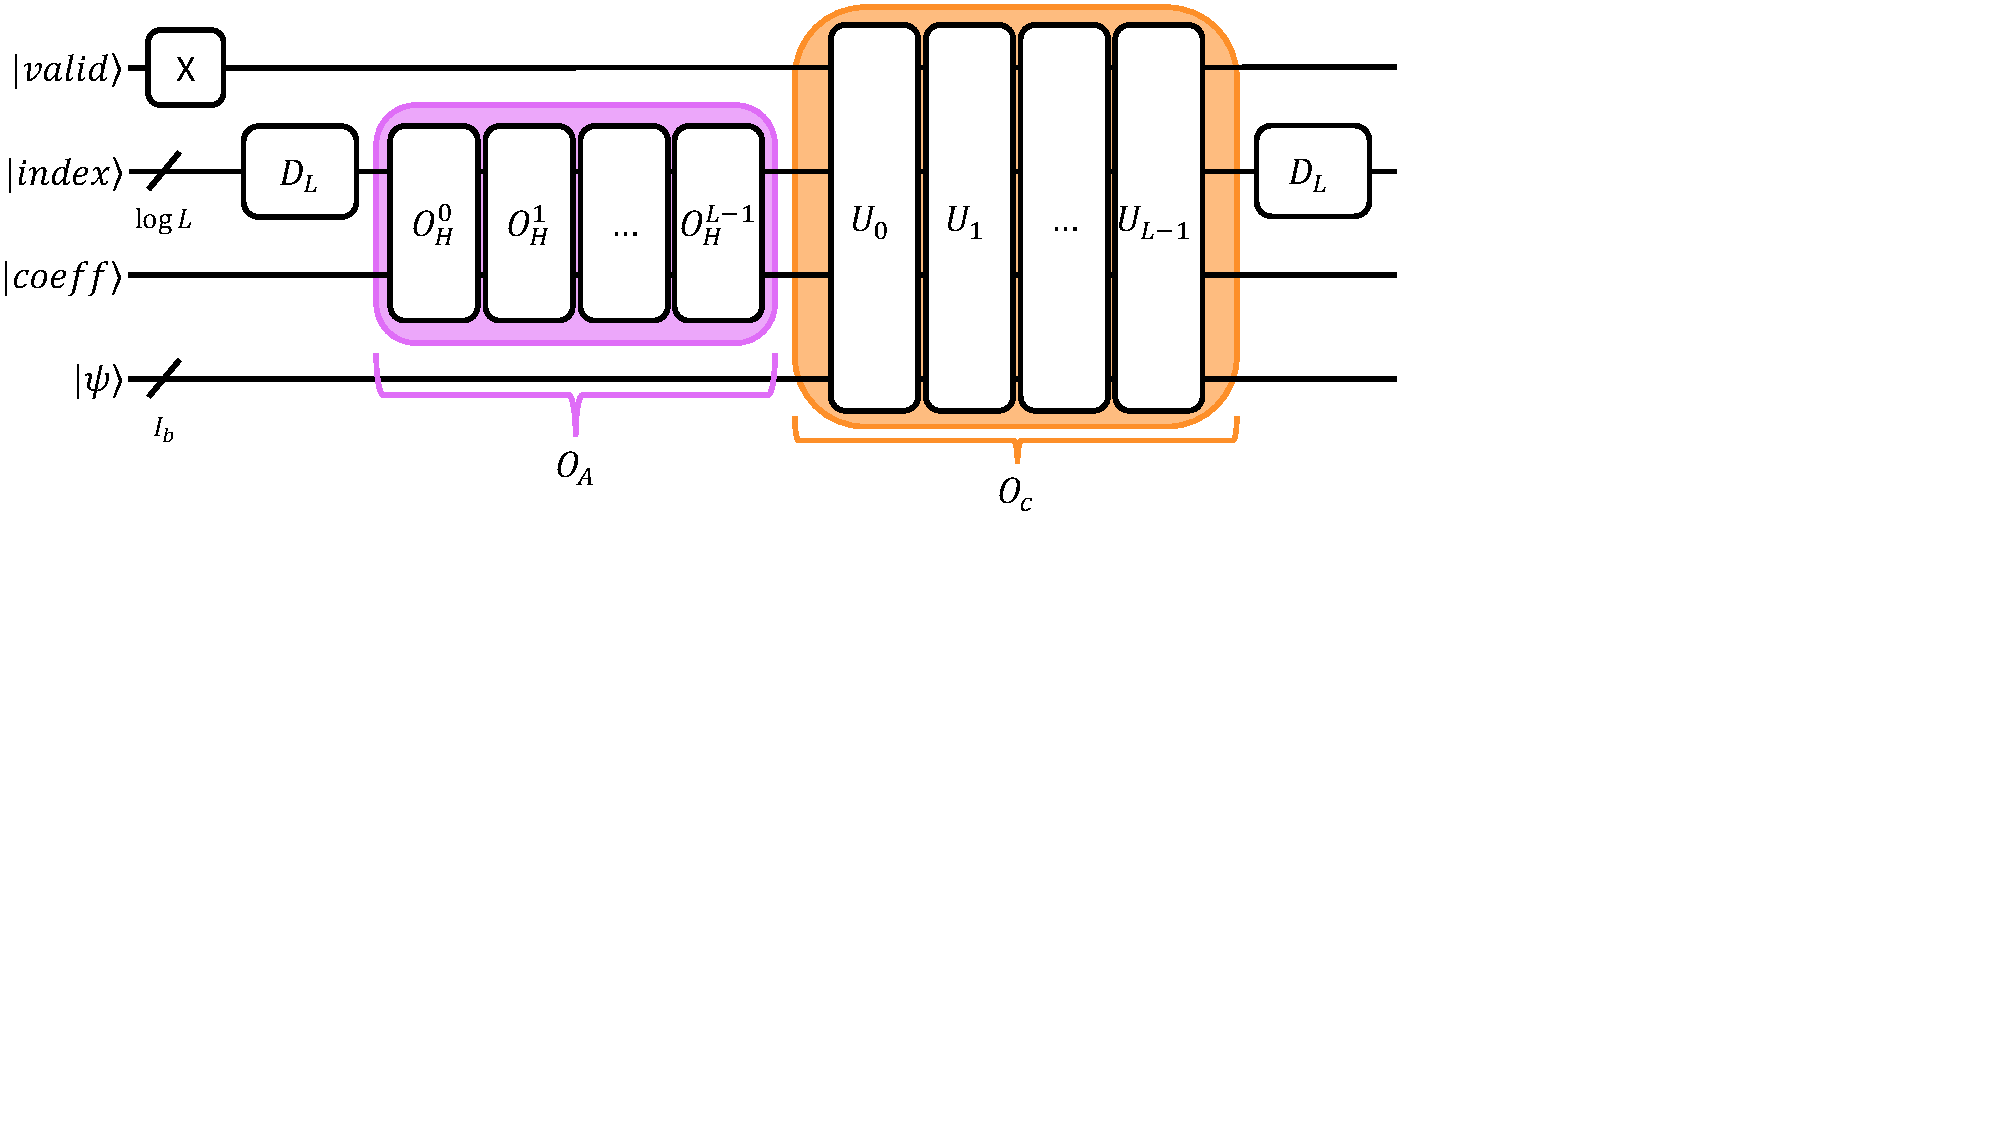
\includegraphics[width=12cm]{figures/liu-construction.pdf}
    \caption{
        \textbf{Sparse-Oracle Block-Encoding Circuit for Pairing Hamiltonians}
        A circuit diagram for the block-encoding described by Liu et. al \cite{liu2024efficient} is shown.
        The $O_A$ oracle is implemented by the series of $O_H^l$ operators (shaded in purple) which load the coefficients of the $l^{th}$ term.
        The $O_c$ oracle is implemented by the series of $U_l$ operators (shaded in orange) which apply the $l^{th}$ term onto the state.
        The $D_L$ oracle represents the diffusion operator (Eq. \ref{eq:diffusion-had}) acting on $L$ terms where $L$ is raised to the nearest power of two.
        The unitary $U_H = D_L O_c O_A D_L$ implements a block-encoding of the pairing Hamiltonian (Eq. \ref{eq:pairing-ham}) assuming the validation qubit ($\ket{\text{valid}}$) is initialized in the $\ket{1}$ state.
        The rescaling factor of this block encoding is given by $\lambda = L \max_{ij} {|h_{ij}|}$.
    }
    \label{fig:liu-construction}
\end{figure}

The structure of the circuits to block-encoding the pairing Hamiltonian is given in Figure \ref{fig:liu-construction}.
The sequence of $O_H^l$ unitaries implement the $O_A$ oracle and the sequence of $U_l$ unitaries implement the $O_c$ oracle.

\begin{figure}[h]
    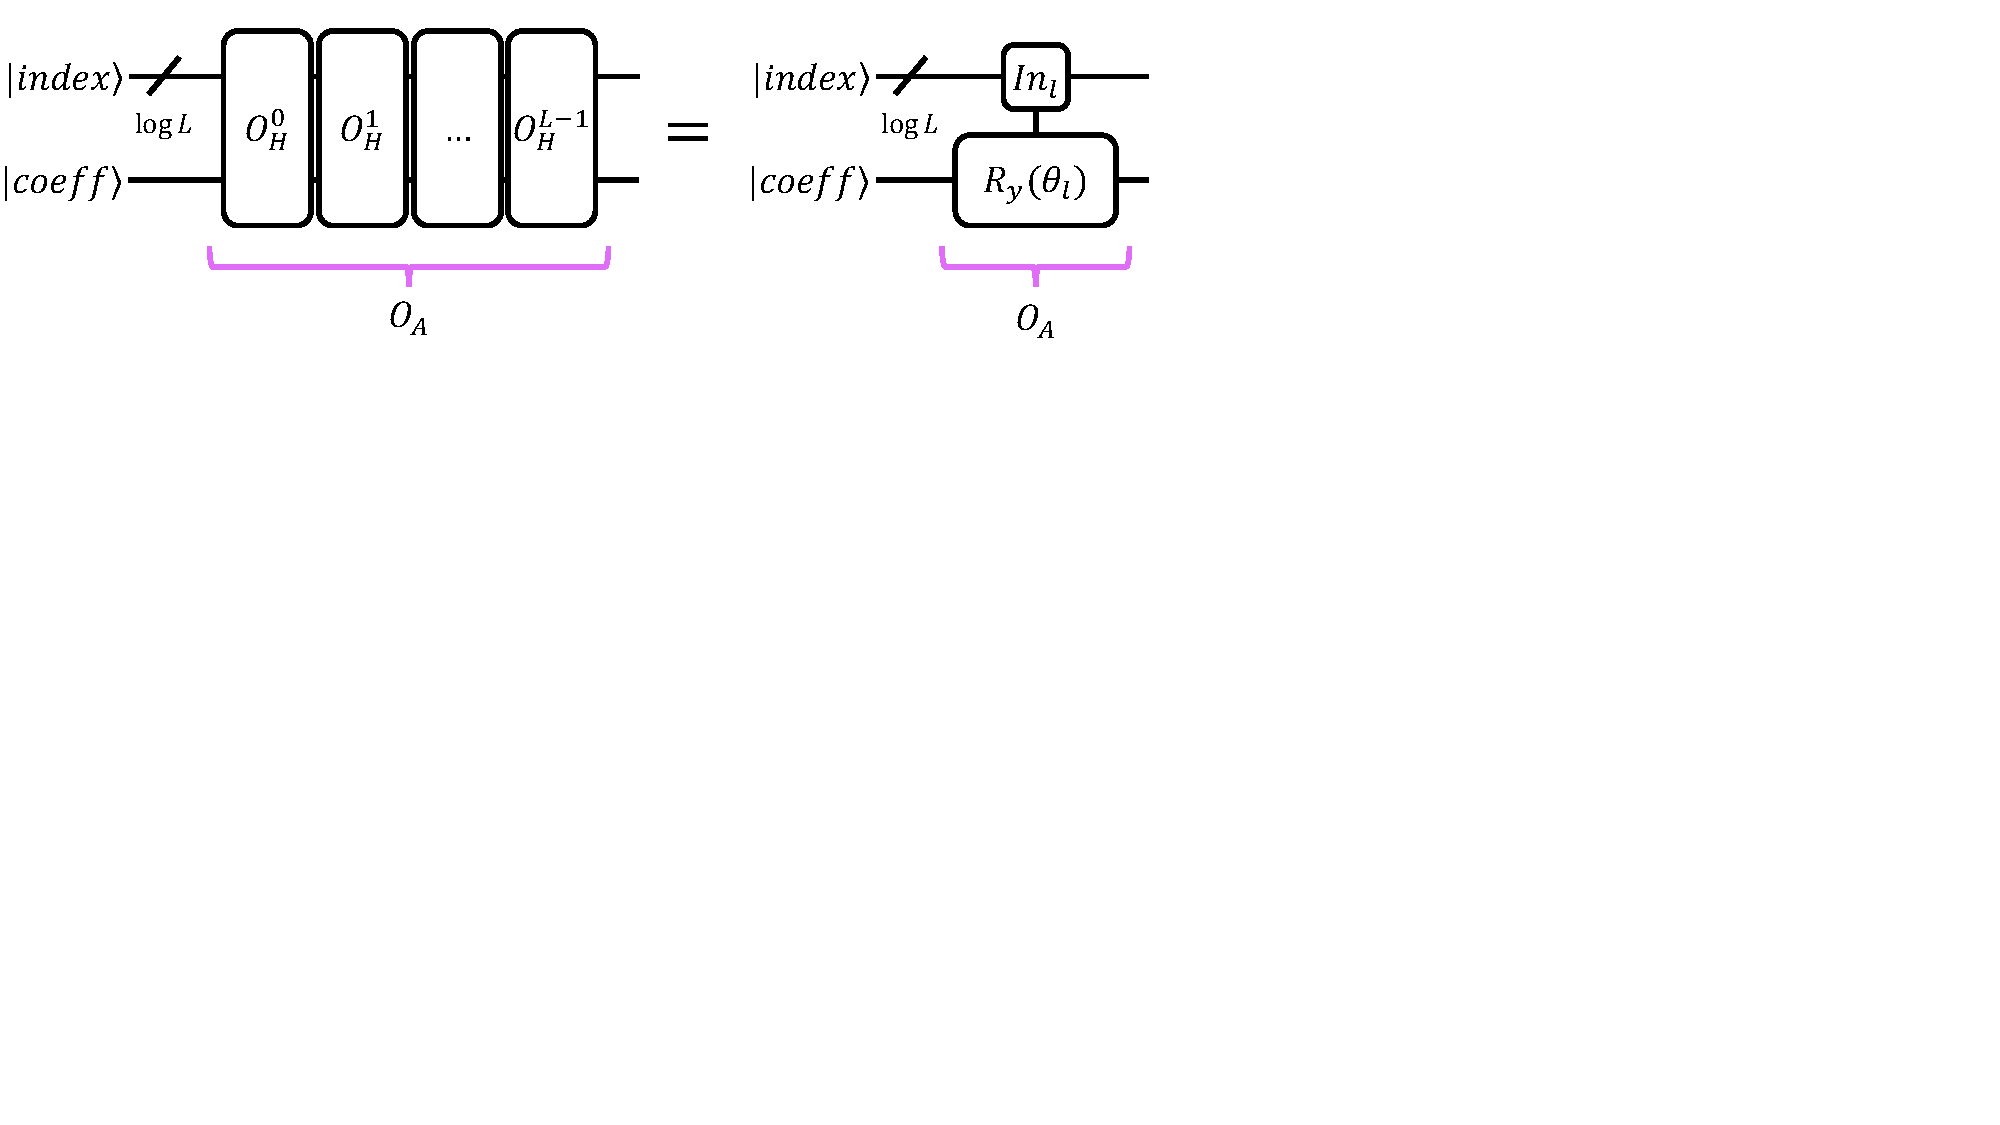
\includegraphics[width=12cm]{figures/liu-O_A.pdf}
    \caption{
        \textbf{$O_A$ Circuit for Pairing Hamiltonians}
        A circuit diagram for the $O_A$ oracle described by Liu et. al \cite{liu2024efficient}.
        Each unitary in the subfigure on the left performs an $R_y$ rotation on the coefficient qubit, controlled on the index register being in the computational basis state $\ket{l}$.
        This sequence of controlled rotations is referred to as a set of uniformly controlled rotations which is depicted by the subfigure on the right.
        Further discussion of compiling uniformly controlled rotations is given in Appendix \ref{sec:multiplexed-rotations}.
    }
    \label{fig:liu-O_A}
\end{figure}

Following Eq. \ref{eq:value-oracle}, the $O_A$ oracle rotates an ancilla qubit ($\ket{\text{coeff}}$ in Figure \ref{fig:liu-construction}) proportionally to the coefficient of the $l^\text{th}$ term when the index register ($\ket{\text{index}}$) is in the computational basis state $\ket{l}$.
This can be achieved by an $R_y$ rotation:
\begin{equation}
    \begin{split}
        & R_y (\theta_l) \ket{0}_\text{coeff} = h_{ij} \ket{0}_\text{coeff} + \sqrt{1 - |h_{ij}|^2} \ket{1}_\text{coeff} \\
        & \theta_l = 2 \cos^{-1}{(h_{ij})}
    \end{split}
\end{equation}
where the rotation is controlled on the index register being in the $l^\text{th}$ computational basis state.

This sequence of rotations controlled on the basis states of the index register is sometimes referred to as a set of uniformly controlled rotations.
When the axis of the rotations is the same for each rotation (as is the case here), the decomposition given by Möttönen et. al \cite{mottonen2004transformation} can be applied.
Under this construction, the $O_A$ oracle can be implemented using $L$ uncontrolled rotations.
A further discussion of this compilation is given in Appendix \ref{sec:multiplexed-rotations}.

The $O_c$ oracle is constructed by the unitaries denoted as $U_0 \dots U_{L - 1}$ in Figure \ref{fig:liu-construction}.
Each unitary $U_l$ is controlled on the index register being in the computational basis state $\ket{l}$.
This series of controlled operations can again be described as a set of uniformly controlled operations where each operation being applied is constructed to apply a block-encoding of the $l^\text{th}$ term in the Hamiltonian onto the system register.

\begin{figure}[h]
    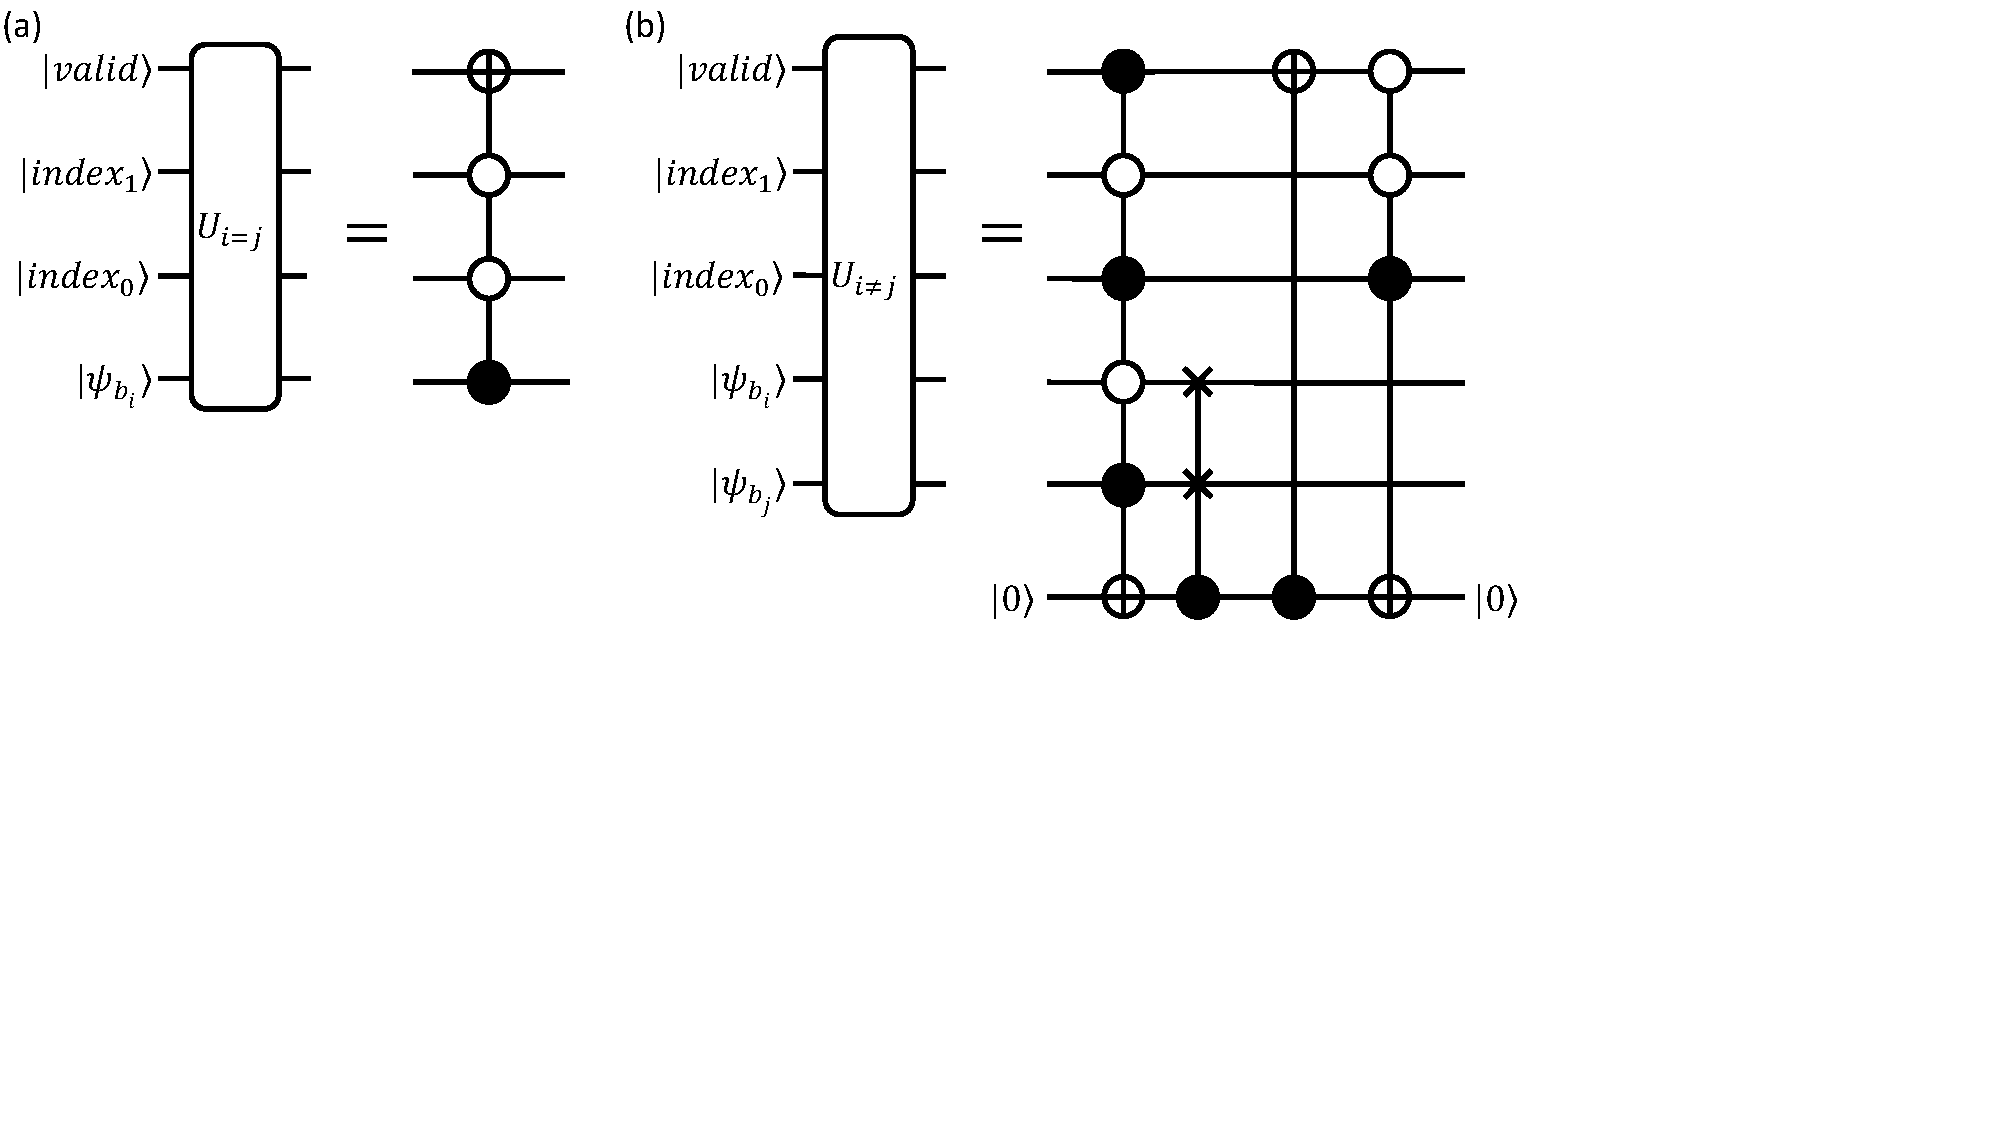
\includegraphics[width=12cm]{figures/liu-O_c.pdf}
    \caption{
        \textbf{$O_c$ Circuit Components for Pairing Hamiltonians}
        A circuit diagram for the unitaries comprising the $O_c$ oracle described by Liu et. al \cite{liu2024efficient} are shown.
        The circuit in subfigure a shows the unitary $U_{i = j}$ which applies a block-encoding of the operator $b_i^\dagger b_i$ when the index register is in the computational basis state $\ket{0}$. 
        The circuit in subfigure a shows the unitary $U_{i \neq j}$ which applies a block-encoding of the operator $b_i^\dagger b_j$ when the index register is in the computational basis state $\ket{1}$. 
    }
    \label{fig:liu-O_c}
\end{figure}

Liu et. al give constructions for applying the terms in the pairing Hamiltonian onto the system under the two cases $i = j$ and $i \neq j$.
In their construction, the validation qubit is initialized in the $\ket{1}$ state and is used to block-encode the individual terms in the Hamiltonian.

When the index for the ladder operators in Eq. \ref{eq:pairing-ham} are the same ($i = j$), the operator $b_i^\dagger b_i$ should zero-out the quantum state when the $i^\text{th}$ mode is unoccupied and should leave the state unchanged when the mode is occupied. 
For these terms, the desired action on the validation qubit is to leave it unaltered when the mode is unoccupied and flip the state of the validation qubit to $\ket{0}$ when the mode is occupied.
This can be achieved by a Toffoli gate which is controlled on the $i^\text{th}$ mode being occupied and the index register being in the computational basis state $\ket{l}$.
An example of these operators is given in Figure 11 of \cite{liu2024efficient} and we give a reproduction in Figure \ref{fig:liu-O_c}a.

When the indices that the ladder operators act on are not the same ($i \neq j$), the operator $b_i^\dagger b_j$ should zero-out the quantum state unless both the $i^\text{th}$ mode is unoccupied \textit{and} the $j^\text{th}$ mode is occupied.
Otherwise, the system of the state would be zeroed-out which would be indicated by leaving the validation qubit unchanged (in the $\ket{1}$ state).
If these conditions are true, a swap gate can be applied to swap the occupations of the fermionic modes and the validation qubit should be flipped to the $\ket{0}$ state. 

To perform this action, an ancillae qubit can be used to store the logical-AND of the conditions on the validation qubit, the index register, and the occupation states of the fermionic modes.
We assume that this ancilla qubit begins in the $\ket{0}$ state and the intent will be to return it to the $\ket{0}$ state such that it can be reused on subsequent operations.
In this work, we refer to qubits that are only temporarily rotated outside of the $\ket{0}$ state as clean ancillae.
An example for a circuit to perform this operation is also given in Figure 11 of \cite{liu2024efficient} and we give a reproduction in Figure \ref{fig:liu-O_c}b.
We note that to properly uncompute the ancilla qubit and return it to the $\ket{0}$ state we include the controls on the index register.
These controls are not present in the constructions given by Liu et. al, but must be included to properly reset this ancilla qubit.
\ws{Determine if construction by Liu et. al is actually incorrect or just incorrect if you want to treat the ancilla qubit as a clean ancilla.}

The controls on the index register for each $U_l$ comprising the $O_c$ oracle ensure that only the $l^\text{th}$ term is applied when the computational basis state is in the $\ket{l}$ state.
These controls on the index register are present for each term and can be accounted for by the uniformly controlled operation structure discussed in more detail in Appendix \ref{sec:uniformly-controlled-operations}.



\subsection{Linear Combination of Unitaries}
\label{subsec:lcu}

Suppose we wish to generate a block-encoding of an operator that can be written as a linear combination of unitary operators:
\begin{equation}
    \label{eq:lcu}
    A = \sum_{l=0}^{L-1} \alpha_l U_l
\end{equation}
where $\alpha_l$ are real-valued coefficients and each $U_l$ is a unitary operator.
The restriction here on real-valued coefficients is simply to be clear about the cost of block-encoding this operator. 
If we wish to include terms with imaginary coefficients, we can absorb the imaginary phase into the operator: $i \alpha_l U_l = \alpha_l U_l^\prime$.
Likewise, a term with a complex coefficient can be treated as two distinct terms ($U_l$ and $U_l^\prime$) each with a real coefficient, though this increases the number of terms ($L$).
\ws{Question: when we decompose a state into a linear combination of other states we say we expand it in some basis. What is the wording for when we expand an operator in a basis of operators?}

Assuming that $A$ is sparse in this description - $L$ grows polynomially with $N_A$ - then the Sparse-Oracle framework generates a valid block-encoding of $A$ where the rescaling factor would be $\lambda = 2^{\lceil \log_2 L \rceil} \max_{l} |\alpha_l|$.
In this construction, $O_A$ would load the (rescaled) coefficients $\{\alpha_l\}$ and $O_c$ would apply the unitaries $\{U_l\}$ onto the system register controlled on the index register being in the computational basis states $\{\ket{l}\}$. 

However, an alternative framework proposed by Childs et. al \cite{childs2012hamiltonian} called Linear Combination of Unitaries (LCU) is \textit{specifically} designed for generating block-encodings of operators in the form of Eq. \ref{eq:lcu}. 
With two oracles, \textit{Prepare} and \textit{Select}, an LCU block-encoding can be defined as follows:
\begin{theorem}
    \label{th:lcu}
    Given a matrix $A$ defined by Eq. \ref{eq:lcu}, let the oracles \textbf{Prepare} and \textbf{Select} be defined by:
    \begin{equation}
        \label{eq:prep-state}
        \textbf{Prepare}\text{:} \ket{0^{\otimes \lceil \log_2 L \rceil}}_\text{index} \rightarrow \sum_{l=0}^{L-1} \sqrt{| \alpha_l | / \lambda} \ket{l}_\text{index}
    \end{equation}
    where $\lambda$ is given by $\lambda_\text{LCU}$ (defined below) and
    \begin{equation}
        \label{eq:select}
        \textbf{Select}\text{:} 
        \begin{cases} 
            \text{Apply $U_l$ on $\ket{\psi}$} & \text{when $\ket{\text{index}}$ is $\ket{l}$} \\
            \text{Undefined} & \text{Otherwise} \\
        \end{cases}
    \end{equation}
    where the \textbf{Select} oracle applies the unitary $U_l$ on the system register when the index register is in the computational basis state $\ket{l}$ and the action is not strictly defined for other states of the index register.

    Then a block-encoding for $A$ is given by:
    \begin{equation}
        \label{eq:lcu-be}
        U_A = (\textbf{Prepare}^\dagger) (\textbf{Select}) (\textbf{Prepare})
    \end{equation}
    with a rescaling factor of:
    \begin{equation}
        \lambda_\text{LCU} = \sum_{l=0}^{L-1} | \alpha_l |
    \end{equation}
\end{theorem}
A simple proof that $U_A$ block-encodes $A$ is given in Section 7.3 of Lin et. al \cite{lin2022lecture}.

The rescaling factor for an LCU block-encoding is given by the 1-norm of the coefficients in Eq. \ref{eq:lcu} and ensures that the corresponding $\bar{U}_l$ has spectral norm less than or equal to $1$.
A benefit of an LCU block-encoding over a Sparse-Oracle block-encoding is the smaller rescaling factor.
A simple proof that $\lambda_\text{LCU} \leq \lambda_\text{SO}$ is given in Appendix \ref{sec:proof-of-rescaling-factors}.

\subsubsection{Implementing \textbf{Prepare}}

The \textit{Prepare} oracle serves a similar role to the $O_A$ oracle in that it loads the coefficients or the values of the matrix elements onto the quantum computer.
The action of the \textit{Prepare} oracle defined by Eq. \ref{eq:prep-state} is to map the all-zero state of an ancilla register to a particular superposition state where the squared amplitudes of the computational basis states are weighted to encode the coefficients of the terms in the operator.
We refer to this ancilla register as the \textit{index register} as the computational basis states of this register, $\ket{l}$, index the $L$ terms in A.

The matrix representation for a valid implementation of the \textit{Prepare} oracle in the computational basis is given by:
\begin{equation}
    \text{Prepare} = \begin{bmatrix}
        \sqrt{|\alpha_0| / \lambda_\text{LCU}} & * & ... & * \\
        \sqrt{|\alpha_1| / \lambda_\text{LCU}} & * & ... & * \\
        \vdots & \vdots & \ddots & \vdots \\
        \sqrt{|\alpha_{L-1} |/ \lambda_\text{LCU}} & * & ... & * \\
    \end{bmatrix}
\end{equation}
From this definition, it is clear that there are infinitely many unitaries that implement the $\textit{Prepare}$ oracle since only the first column of the operator is fixed.

For operators that have structure among the coefficients of the terms, implementations of $\textit{Prepare}$ can be constructed that leverage this structure to reduce the time cost of implementing the oracle.
In certain cases, this can drastically reduce the cost such as is done for the Fermi-Hubbard model in \cite{babbush2018encoding} where there are only two unique coefficients in the LCU.

When a certain structure is not present, the Grover-Rudolph algorithm \cite{grover2002creating} gives a formulaic routine to generate quantum circuits that implement the $\textit{Prepare}$ oracle.
Although the cost of implementing Grover-Rudolph scales exponentially with the number of qubits in the register it acts upon, the size of the index register is logarithmic in the number of terms in the operator being block-encoded.
Therefore, the cost of Grover-Rudolph will be linear in $L$.
If A is \textit{sparse} - $L$ grows polynomially with respect to $N_A$ - then the cost of Grover-Rudolph will be polynomial with respect to $N_A$.  

\subsubsection{Implementing \textbf{Select}}

Similar to the $O_c$ oracle, the desired action of the \textit{Select} oracle is to apply the unitary $U_l$ onto the system register \textit{controlled} on the index regsiter being in the state $\ket{l}$ (Eq. \ref{eq:select}).
Since the action of the \textit{Select} oracle is undefined when the computational basis states of the index register is greater than $L - 1$, there are also infinitely many valid quantum circuits for implementing \textit{Select}.

\begin{figure}[h]
    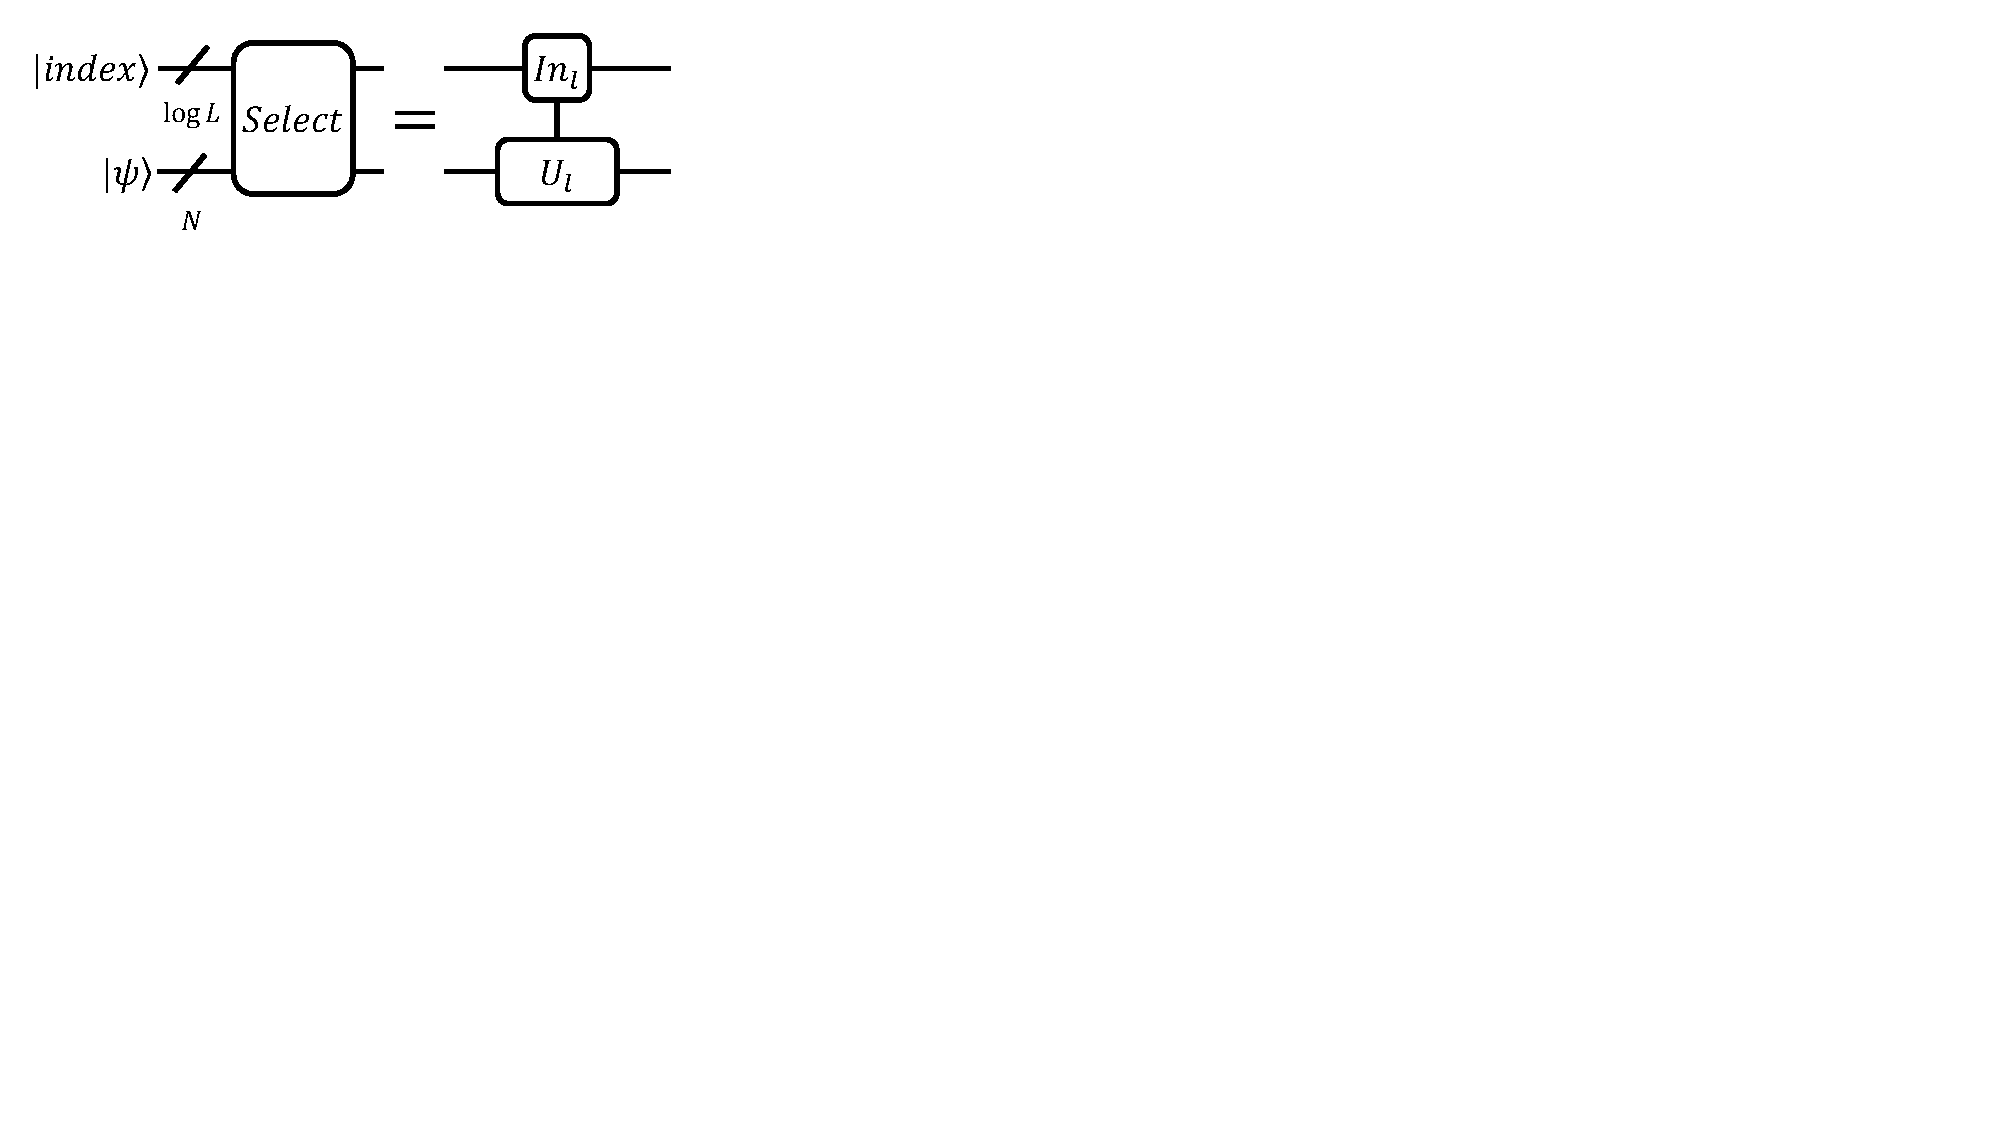
\includegraphics[width=6cm]{figures/select-lcu.pdf}
    \caption{
        \textbf{LCU \textit{Select} Oracle}
        A circuit diagram for the \textit{Select} oracle in LCU is shown.
        This is a naive implementation where no structure in the operator is assumed.
        The \textit{Select} oracle applies the $l^\text{th}$ unitary in the LCU (Eq. \ref{eq:lcu}) onto the system when the index register is in the computational basis state $\ket{l}$
        This can be achieved using a set of uniformly controlled operations (right subfigure).
    }
    \label{fig:unstructured-select}
\end{figure}

If structure in the problem is present, the \textit{Select} oracle can be implemented to leverage that structure as is done in \cite{babbush2018encoding}.
Without any assumptions on the structure in $A$, the \textit{Select} oracle can be implemented by the operator:
\begin{equation}
    \label{eq:select-naive}
    \text{Select} = \sum_{l=0}^{L-1} \ket{l}\bra{l} \otimes U_l
\end{equation}
Similar to the $O_A$ and $O_c$ oracles, the \textit{Select} oracle serially controls upon the computational basis states of the index register and this control structure can be grouped together as a uniformly controlled operation which is discussd in more detail in Appendix \ref{sec:uniformly-controlled-operations}.
This is shown in Figure \ref{fig:unstructured-select}.

As a quick aside, if the implementation of the \textit{Select} oracle is self-inverse, then the LCU block-encoding is also self-inverse.
This structure makes LCU block-encodings particularly well-suited for being applied in algorithms based on Qubitization \cite{low2019hamiltonian}.
Using the construction for \textit{Select} in Eq. \ref{eq:select-naive}, the implementation will be self-inverse if the unitaries themselves are self-inverse.
As an example, this is the case for when the operator $A$ is decomposed in the Pauli basis as the Paulis are self-inverse. 

\subsection{Linear Combination of Operators}
\label{subsec:unification}

LCU block-encodings provide better rescaling factors, yet there are clearly parallels between the $O_A$ oracle and the \textit{Prepare} oracle, as well as the $O_c$ oracle and the \textit{Select} oracle.
Therefore one might ask if we can construct LCU-style block-encodings for a linear combination of \textit{operators} under the assumption that we have access to block-encodings of each operator:
\begin{equation}
    \label{eq:lco}
    A = \sum_{l=0}^{L-1} \alpha_l O_l
\end{equation}
where the $O_l$ are operators and we again restrict the coefficients $\alpha_l$ to be real-valued for simplicity, yet the same strategies to apply operators with imaginary or complex-valued coefficients used for an LCU can be applied here.
% We also restrict the spectral norms of the operators to satisfy $|\bar{O}_l| \leq 1$ for simplicity and note that we can rescale any operator to satisfy this condition and let the rescaling factor be absorbed by the corresponding coefficient.
% However, we note that extra care must be taken when absorbing these rescaling factors such that the rescaling of the linear combination is consistent across all terms.

Another way to frame this is creating an LCU block-encoding where the unitary operators themselves are block-encodings of operators which is described in Section 4.3 of Gilyén et. al \cite{gilyen2019quantum} and noted by Jennings et. al \cite{jennings2023efficient}.
We will refer to this method of block-encoding as an LCO block-encoding (Linear Combination of Operators).
As noted by Jennings et. al \cite{jennings2023efficient} it may be enlightening to consider an LCU block-encoding as a apecial case of an LCO block-encoding wherein the operators in the linear combination are all unitary.

\begin{theorem}
    \label{th:lco}
    Given a matrix $A$ defined by Eq. \ref{eq:lco} and unitary operators $U_l$ that each block-encode the operators $O_l$:
    \begin{equation}
        \label{eq:applying-operator}
        U_l \ket{\psi}\ket{0}_\text{anc} = \bar{O}_l \ket{\psi} \ket{0}_\text{anc} + \beta_{\psi, l} \ket{\perp}
    \end{equation}
    with rescaling factors $\lambda_l$ such that $\lambda_l \bar{O}_l = O_l$.
    
    Define the \textbf{Prepare} oralce by:
    \begin{equation}
        \label{eq:prep-lco}
        \textbf{Prepare}\text{:} \ket{0^{\otimes \lceil \log_2 L \rceil}}_\text{index} \rightarrow \sum_{l=0}^{L-1} \sqrt{| \bar{\alpha}_l | / \lambda} \ket{l}_\text{index}
    \end{equation}
    where $\bar{\alpha_l}$ is given by:
    \begin{equation}
        \label{eq:rescaled-coeffs}
        \bar{\alpha_l} = \frac{\alpha_l \lambda_l}{\max_{l^\prime}{\lambda_{l^\prime}}}
    \end{equation}
    and $\lambda$ is given by:
    \begin{equation}
        \lambda = \sum_{l=0}^{L-1} \bar{\alpha_l}
    \end{equation}

    Define the \textbf{Select} oracle by:
    \begin{equation}
        \label{eq:select-conditions-lco}
        \textbf{Select}\text{:} 
        \begin{cases} 
            \text{Apply $U_l$ on $\ket{\psi}\ket{0}_\text{anc}$} & \text{when $\ket{\text{index}}$ is $\ket{l}$} \\
            \text{Undefined} & \text{Otherwise} \\
        \end{cases}
    \end{equation}
    where the \textbf{Select} oracle applies a block-encoding of $O_l$ on the system register using an additional ancilla register when the index register is in the computational basis state $\ket{l}$ and the action is not strictly defined for other states of the index register.

    Then a block-encoding for $A$ is given by:
    \begin{equation}
        \label{eq:lco-be}
        U_A = (\textbf{Prepare}^\dagger) (\textbf{Select}) (\textbf{Prepare})
    \end{equation}
    with a rescaling factor of:
    \begin{equation}
        \lambda_\text{LCO} = \big(\max_{l}{\lambda_l}\big) \sum_{l=0}^{L-1} | \bar{\alpha}_l | = \sum_{l=0}^{L-1} |\alpha_l \lambda_l|
    \end{equation}
\end{theorem}
The proof that $U_A$ block-encodes $A$ follows from the same proof for LCU block-encodings given by Lin et. al \cite{lin2022lecture}.

To motivate that this rescaling factor is more favorable than a Sparse-Oracle block-encoding, consider the case of the pairing Hamiltonian.
Using the construction given by Liu et. al, the rescaling factor for $H$ is given by:
\begin{equation}
    \lambda_\text{SO}^H = 2^{\lceil \log_2 L \rceil} \max_{ij} |h_{ij}|
\end{equation}
Since each operator in Eq. \ref{eq:pairing-ham} has a spectral norm of $1$, then the rescaling for an LCO block-encoding is simply given by:
\begin{equation}
    \lambda_\text{LCO}^H = \sum_{ij} |h_{ij}|
\end{equation}
and the proof that $\lambda_\text{LCO}^H \leq \lambda_\text{SO}^H$ follows directly from the proof given in Appendix \ref{sec:proof-of-rescaling-factors}.

Implementing the LCO \textit{Prepare} and \textit{Select} oracles can be done similarly to the LCU oracles.
The \textit{Prepare} oracle follows directly from LCU using the rescaled coefficients $\{\bar{\alpha}_l\}$ defined by Eq. \ref{eq:rescaled-coeffs}. 
If structure among the coefficients is present, then this structure can be exploited. 
If no structure exists, then the Grover-Rudolph algorithm can be applied.

The construction for \textit{Select} can again leverage the problem structure if such a structure exists, or it can be generated using uniformly controlled operations following:
\begin{equation}
    \label{eq:select-lco}
    \text{Select} = \sum_{l=0}^{L-1} \ket{l}\bra{l} \otimes U_l
\end{equation}
where the block-encodings for the operators $O_l$ can be constructed using any of the frameworks discussed here.
\section{Compiling Ladder Operator Block-Encodings}
\label{sec:ladder-op-oracles}

In this work, we focus on generating block-encodings for second-quantized Hamiltonians that include both fermionic and bosonic ladder operators.
In this section, we provide a framework and explicit compilations for controlled block-encodings of different products and linear combinations of ladder operators.
For our compilations, we primarily reduce the number of non-Clifford operations and secondarily reduce the number of block-encoding ancillae at the expense of temporary, clean ancillae.

\subsection{Encoding}
\label{subsec:encoding}

The encoding that is used for the occupation of the fermionic modes is identical to the Jordan-Wigner encoding \cite{jordan-wigner}.
The map between a Fock state to a qubit state is given as 
\begin{equation}
    \ket{n_{I_b}, \dots, n_{1_b}, n_{0_b}} \rightarrow \ket{q_{I_b}, \dots, q_{1_b}, q_{0_b}}
\end{equation}
where $n_{i_b} = q_{i_b} \in [0, 1]$ depending on if mode $i$ is occupied ($\ket{1}$) or unoccupied ($\ket{0}$).
The number of qubits required for the fermionic system is equal to the number of fermionic modes.

The encoding scheme for bosons must allow for occupancies in the range $[0, \Omega]$ due to the absence of the Pauli exclusion principle.
We choose to represent store the occupancy of a bosonic mode in binary notation: 
\begin{equation}
    \ket{n_{i_a}} \rightarrow \ket{b_j, b_{j-1}, ..., b_0}
\end{equation}
where $j$ runs from $0$ to $\lceil \log_2{\Omega} \rceil - 1$ and the values of $b_j$ are given by the binary representation of $n_{i_a}$.
This is identical to the encoding used in \cite{rhodes2024exponential}. \ws{check citation}

Storing the occupation of each bosonic mode requires $\lceil \log_2{\Omega} \rceil$ qubits if we assume that the maximum bosonic occupation is the same for each bosonic mode.
This choice of the maximum bosonic occupation being constant for all bosonic modes is not a restriction of the methods presented in this work, but is chosen for simplicity. 
With this choice, the number of qubits required for the bosonic subsystem is: $Q_{\psi_a} = I_a \lceil \log_2{\Omega} \rceil$.

\subsection{Fermionic Ladder Operators}
\label{subsec:fermionic-be}

Here, we aim to define a family of unitaries ($\{U_{b^\dagger_j}, U_{b_j}\}$) that generate block-encodings of the associated fermionic creation ($b_j^\dagger$) and annihilation ($b_j$) operators.
As these are block-encodings of non-unitary operators, we define the associated unitary operators to be of the form of Eq. \ref{eq:general-block-encoding}:
\begin{equation}
    U_{b^\dagger_j} \ket{\psi} \ket{0}_\text{anc} = b^\dagger_j \ket{\psi}\ket{0}_\text{anc} + \beta_\psi \ket{\perp}
\end{equation}
No rescaling factor is needed for these operators since the fermionic ladder operators have spectral norm of $1$.

The definition of the fermionic creation operator (Eq. \ref{eq:fermionic-creation}) creates two implications.
If the mode is unoccupied, then the mode should become occupied and a sign should be applied based on the occupancy of the preceeding fermionic modes.
If the mode is occupied, then state should be zeroed-out. 
Therefore, the action of our unitary will be dependent on the occupation of the fermionic mode:
\begin{equation}
    U_{b^\dagger_j} \ket{\psi_j} \ket{0}_\text{anc} =
    \begin{cases} 
        \ket{1} \ket{0}_\text{anc} & \text{when $\ket{\psi_j}$ is $\ket{0}$} \\
        \ket{\perp} & \text{when $\ket{\psi_j}$ is $\ket{1}$} \\
    \end{cases}
\end{equation}
where the sign flip caused by the occupation of the preceeding modes is omitted for brevity, but is assumed throughout the remainder of this section.

\begin{figure}[h]
    \mbox{
        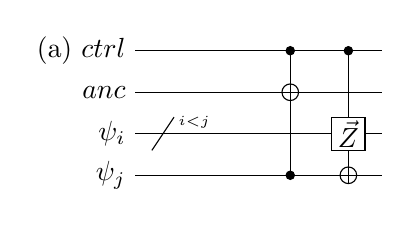
\begin{tikzpicture}[scale=1.000000,x=1pt,y=1pt]
\filldraw[color=white] (0.000000, -7.500000) rectangle (89.000000, 52.500000);
% Drawing wires
% Line 1: ctrl W \text{(a) }ctrl
\draw[color=black] (0.000000,45.000000) -- (89.000000,45.000000);
\draw[color=black] (0.000000,45.000000) node[left] {$\text{(a) }ctrl$};
% Line 2: anc W anc
\draw[color=black] (0.000000,30.000000) -- (89.000000,30.000000);
\draw[color=black] (0.000000,30.000000) node[left] {$anc$};
% Line 3: i W \psi_i
\draw[color=black] (0.000000,15.000000) -- (89.000000,15.000000);
\draw[color=black] (0.000000,15.000000) node[left] {$\psi_i$};
% Line 4: j W \psi_j
\draw[color=black] (0.000000,0.000000) -- (89.000000,0.000000);
\draw[color=black] (0.000000,0.000000) node[left] {$\psi_j$};
% Done with wires; drawing gates
% Line 6: i / ^{i<j}
\draw (6.000000, 9.000000) -- (14.000000, 21.000000);
\draw (12.000000, 18.000000) node[right] {$\scriptstyle{^{i<j}}$};
% Line 7: ctrl anc i j LABEL
% Line 8: ctrl j +anc
\draw (56.000000,45.000000) -- (56.000000,0.000000);
\filldraw (56.000000, 45.000000) circle(1.500000pt);
\filldraw (56.000000, 0.000000) circle(1.500000pt);
\begin{scope}
\draw[fill=white] (56.000000, 30.000000) circle(3.000000pt);
\clip (56.000000, 30.000000) circle(3.000000pt);
\draw (53.000000, 30.000000) -- (59.000000, 30.000000);
\draw (56.000000, 27.000000) -- (56.000000, 33.000000);
\end{scope}
% Line 10: i G $\vec{Z}$ ctrl +j
\draw (77.000000,45.000000) -- (77.000000,0.000000);
\begin{scope}
\draw[fill=white] (77.000000, 15.000000) +(-45.000000:8.485281pt and 8.485281pt) -- +(45.000000:8.485281pt and 8.485281pt) -- +(135.000000:8.485281pt and 8.485281pt) -- +(225.000000:8.485281pt and 8.485281pt) -- cycle;
\clip (77.000000, 15.000000) +(-45.000000:8.485281pt and 8.485281pt) -- +(45.000000:8.485281pt and 8.485281pt) -- +(135.000000:8.485281pt and 8.485281pt) -- +(225.000000:8.485281pt and 8.485281pt) -- cycle;
\draw (77.000000, 15.000000) node {$\vec{Z}$};
\end{scope}
\filldraw (77.000000, 45.000000) circle(1.500000pt);
\begin{scope}
\draw[fill=white] (77.000000, 0.000000) circle(3.000000pt);
\clip (77.000000, 0.000000) circle(3.000000pt);
\draw (74.000000, 0.000000) -- (80.000000, 0.000000);
\draw (77.000000, -3.000000) -- (77.000000, 3.000000);
\end{scope}
% Done with gates; drawing ending labels
% Done with ending labels; drawing cut lines and comments
% Done with comments
\end{tikzpicture}

        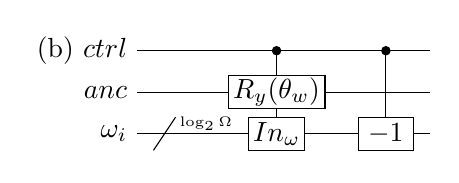
\begin{tikzpicture}[scale=1.000000,x=1pt,y=1pt]
\filldraw[color=white] (0.000000, -7.500000) rectangle (106.000000, 37.500000);
% Drawing wires
% Line 1: ctrl W \text{(b) }ctrl
\draw[color=black] (0.000000,30.000000) -- (106.000000,30.000000);
\draw[color=black] (0.000000,30.000000) node[left] {$\text{(b) }ctrl$};
% Line 2: anc W anc
\draw[color=black] (0.000000,15.000000) -- (106.000000,15.000000);
\draw[color=black] (0.000000,15.000000) node[left] {$anc$};
% Line 3: i W \omega_i
\draw[color=black] (0.000000,0.000000) -- (106.000000,0.000000);
\draw[color=black] (0.000000,0.000000) node[left] {$\omega_i$};
% Done with wires; drawing gates
% Line 5: i / ^{\log_2{\Omega}}
\draw (6.000000, -6.000000) -- (14.000000, 6.000000);
\draw (12.000000, 3.000000) node[right] {$\scriptstyle{^{\log_2{\Omega}}}$};
% Line 6: ctrl anc i LABEL width=-5
% Line 8: anc G:width=35 $R_y(\theta_w)$ i G:width=20 $In_\omega$ ctrl
\draw (50.500000,30.000000) -- (50.500000,0.000000);
\begin{scope}
\draw[fill=white] (50.500000, 15.000000) +(-45.000000:24.748737pt and 8.485281pt) -- +(45.000000:24.748737pt and 8.485281pt) -- +(135.000000:24.748737pt and 8.485281pt) -- +(225.000000:24.748737pt and 8.485281pt) -- cycle;
\clip (50.500000, 15.000000) +(-45.000000:24.748737pt and 8.485281pt) -- +(45.000000:24.748737pt and 8.485281pt) -- +(135.000000:24.748737pt and 8.485281pt) -- +(225.000000:24.748737pt and 8.485281pt) -- cycle;
\draw (50.500000, 15.000000) node {$R_y(\theta_w)$};
\end{scope}
\begin{scope}
\draw[fill=white] (50.500000, -0.000000) +(-45.000000:14.142136pt and 8.485281pt) -- +(45.000000:14.142136pt and 8.485281pt) -- +(135.000000:14.142136pt and 8.485281pt) -- +(225.000000:14.142136pt and 8.485281pt) -- cycle;
\clip (50.500000, -0.000000) +(-45.000000:14.142136pt and 8.485281pt) -- +(45.000000:14.142136pt and 8.485281pt) -- +(135.000000:14.142136pt and 8.485281pt) -- +(225.000000:14.142136pt and 8.485281pt) -- cycle;
\draw (50.500000, -0.000000) node {$In_\omega$};
\end{scope}
\filldraw (50.500000, 30.000000) circle(1.500000pt);
% Line 9: i G width=20 $-1$ ctrl
\draw (90.000000,30.000000) -- (90.000000,0.000000);
\begin{scope}
\draw[fill=white] (90.000000, -0.000000) +(-45.000000:14.142136pt and 8.485281pt) -- +(45.000000:14.142136pt and 8.485281pt) -- +(135.000000:14.142136pt and 8.485281pt) -- +(225.000000:14.142136pt and 8.485281pt) -- cycle;
\clip (90.000000, -0.000000) +(-45.000000:14.142136pt and 8.485281pt) -- +(45.000000:14.142136pt and 8.485281pt) -- +(135.000000:14.142136pt and 8.485281pt) -- +(225.000000:14.142136pt and 8.485281pt) -- cycle;
\draw (90.000000, -0.000000) node {$-1$};
\end{scope}
\filldraw (90.000000, 30.000000) circle(1.500000pt);
% Done with gates; drawing ending labels
% Done with ending labels; drawing cut lines and comments
% Done with comments
\end{tikzpicture}

    }
    \caption{
        \textbf{Fermionic Ladder Operator Block-Encodings}
        In subfigure a, a block-encoding for the fermionic creation operator acting on the $j^\text{th}$ mode is given.
        In subfigure b, a block-encoding for the fermionic annihilation operator acting on the $j^\text{th}$ mode is given.
        For a creation (annihilation) operator, the branch of the wavefunction will be flipped outside of the encoded subspace if the mode is occupied (unoccupied).
        The state is updated by applying Pauli $Z$ gates to the preceeding fermionic modes to apply the appropriate sign and then applying a Pauli $X$ gate to flip the occupation of the $j^\text{th}$ mode.
    }
    \label{fig:fermionic-be}
\end{figure}


A valid construction for $U_{b^\dagger_j}$ is given in subfigure \ref{fig:fermionic-be}a.
The initial Toffoli gate flips the ancilla qubit to indicate that the state has been zeroed-out when the control qubit is on ($\ket{1}$) and the fermionic mode is occupied ($\ket{1}$).
Regardless of the state of the block-encoding ancilla qubit, the sign of the output state can be applied appropriately using a series of controlled Pauli $Z$ operators applied to each of the fermionic modes with index $i < j$: $\vec{Z}_i$.
The occupation of the fermionic mode on which the ladder operator acts upon is updated using a controlled Pauli $X$ operator: $X_j$.

A block-encoding for the fermionic annihilation operator, $U_{b_j}$, can be constructed similarly to $U_{b^\dagger_j}$ and is shown in subfigue \ref{fig:fermionic-be}b.
The fermionic creation operator only acts nontrivially when the mode is \textit{unoccupied}.
Inversely, the fermionic annihilation operator will only act nontrivially if the mode is \textit{occupied}.
Therefore the block-encoding ancilla is flipped outside of the encoded subspace if the control qubit is on ($\ket{1}$) and the fermionic mode is unoccupied.
These constructions have an optimal rescaling factor ($\lambda = 1$), require one block-encoding ancilla, and use one Toffoli gate.

\subsection{Products of Fermionic Ladder Operators}

As discussed in subsection \ref{subsec:be-products}, a block-encoding for a product of operators can be constructed using a product of the unitaries that block-encode each operator.
In this subsection, we construct block-encodings for a product of fermionic ladder operators that use fewer quantum resources than are required by this naive strategy.

\begin{figure}[h]
    \mbox{
        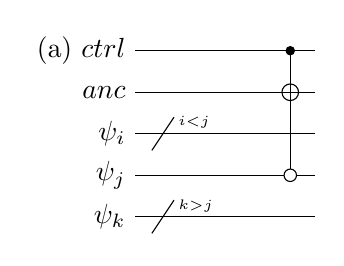
\begin{tikzpicture}[scale=1.000000,x=1pt,y=1pt]
\filldraw[color=white] (0.000000, -7.500000) rectangle (65.000000, 67.500000);
% Drawing wires
% Line 1: ctrl W \text{(a) }ctrl
\draw[color=black] (0.000000,60.000000) -- (65.000000,60.000000);
\draw[color=black] (0.000000,60.000000) node[left] {$\text{(a) }ctrl$};
% Line 2: anc W anc
\draw[color=black] (0.000000,45.000000) -- (65.000000,45.000000);
\draw[color=black] (0.000000,45.000000) node[left] {$anc$};
% Line 3: i W \psi_i
\draw[color=black] (0.000000,30.000000) -- (65.000000,30.000000);
\draw[color=black] (0.000000,30.000000) node[left] {$\psi_i$};
% Line 4: j W \psi_j
\draw[color=black] (0.000000,15.000000) -- (65.000000,15.000000);
\draw[color=black] (0.000000,15.000000) node[left] {$\psi_j$};
% Line 5: k W \psi_k
\draw[color=black] (0.000000,0.000000) -- (65.000000,0.000000);
\draw[color=black] (0.000000,0.000000) node[left] {$\psi_k$};
% Done with wires; drawing gates
% Line 7: i / ^{i<j}
\draw (6.000000, 24.000000) -- (14.000000, 36.000000);
\draw (12.000000, 33.000000) node[right] {$\scriptstyle{^{i<j}}$};
% Line 8: k / ^{k>j}
\draw (6.000000, -6.000000) -- (14.000000, 6.000000);
\draw (12.000000, 3.000000) node[right] {$\scriptstyle{^{k>j}}$};
% Line 9: ctrl anc i j k LABEL
% Line 10: -j +anc ctrl
\draw (56.000000,60.000000) -- (56.000000,15.000000);
\draw[fill=white] (56.000000, 15.000000) circle(2.250000pt);
\begin{scope}
\draw[fill=white] (56.000000, 45.000000) circle(3.000000pt);
\clip (56.000000, 45.000000) circle(3.000000pt);
\draw (53.000000, 45.000000) -- (59.000000, 45.000000);
\draw (56.000000, 42.000000) -- (56.000000, 48.000000);
\end{scope}
\filldraw (56.000000, 60.000000) circle(1.500000pt);
% Done with gates; drawing ending labels
% Done with ending labels; drawing cut lines and comments
% Done with comments
\end{tikzpicture}

        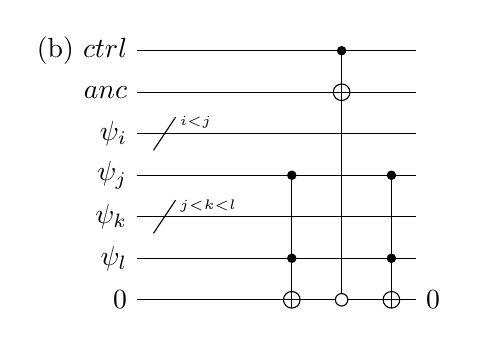
\begin{tikzpicture}[scale=1.000000,x=1pt,y=1pt]
\filldraw[color=white] (0.000000, -7.500000) rectangle (101.000000, 97.500000);
% Drawing wires
% Line 1: ctrl W \text{(b) }ctrl
\draw[color=black] (0.000000,90.000000) -- (101.000000,90.000000);
\draw[color=black] (0.000000,90.000000) node[left] {$\text{(b) }ctrl$};
% Line 2: anc W anc
\draw[color=black] (0.000000,75.000000) -- (101.000000,75.000000);
\draw[color=black] (0.000000,75.000000) node[left] {$anc$};
% Line 3: i W \psi_i
\draw[color=black] (0.000000,60.000000) -- (101.000000,60.000000);
\draw[color=black] (0.000000,60.000000) node[left] {$\psi_i$};
% Line 4: j W \psi_j
\draw[color=black] (0.000000,45.000000) -- (101.000000,45.000000);
\draw[color=black] (0.000000,45.000000) node[left] {$\psi_j$};
% Line 5: k W \psi_k
\draw[color=black] (0.000000,30.000000) -- (101.000000,30.000000);
\draw[color=black] (0.000000,30.000000) node[left] {$\psi_k$};
% Line 6: l W \psi_l
\draw[color=black] (0.000000,15.000000) -- (101.000000,15.000000);
\draw[color=black] (0.000000,15.000000) node[left] {$\psi_l$};
% Line 7: clean0 W 0 0
\draw[color=black] (0.000000,0.000000) -- (101.000000,0.000000);
\draw[color=black] (0.000000,0.000000) node[left] {$0$};
% Done with wires; drawing gates
% Line 9: i / ^{i<j}
\draw (6.000000, 54.000000) -- (14.000000, 66.000000);
\draw (12.000000, 63.000000) node[right] {$\scriptstyle{^{i<j}}$};
% Line 10: k / ^{j<k<l}
\draw (6.000000, 24.000000) -- (14.000000, 36.000000);
\draw (12.000000, 33.000000) node[right] {$\scriptstyle{^{j<k<l}}$};
% Line 11: ctrl anc i j k l clean0 LABEL
% Line 12: j l +clean0
\draw (56.000000,45.000000) -- (56.000000,0.000000);
\filldraw (56.000000, 45.000000) circle(1.500000pt);
\filldraw (56.000000, 15.000000) circle(1.500000pt);
\begin{scope}
\draw[fill=white] (56.000000, 0.000000) circle(3.000000pt);
\clip (56.000000, 0.000000) circle(3.000000pt);
\draw (53.000000, 0.000000) -- (59.000000, 0.000000);
\draw (56.000000, -3.000000) -- (56.000000, 3.000000);
\end{scope}
% Line 13: -clean0 ctrl +anc
\draw (74.000000,90.000000) -- (74.000000,0.000000);
\draw[fill=white] (74.000000, 0.000000) circle(2.250000pt);
\filldraw (74.000000, 90.000000) circle(1.500000pt);
\begin{scope}
\draw[fill=white] (74.000000, 75.000000) circle(3.000000pt);
\clip (74.000000, 75.000000) circle(3.000000pt);
\draw (71.000000, 75.000000) -- (77.000000, 75.000000);
\draw (74.000000, 72.000000) -- (74.000000, 78.000000);
\end{scope}
% Line 14: j l +clean0
\draw (92.000000,45.000000) -- (92.000000,0.000000);
\filldraw (92.000000, 45.000000) circle(1.500000pt);
\filldraw (92.000000, 15.000000) circle(1.500000pt);
\begin{scope}
\draw[fill=white] (92.000000, 0.000000) circle(3.000000pt);
\clip (92.000000, 0.000000) circle(3.000000pt);
\draw (89.000000, 0.000000) -- (95.000000, 0.000000);
\draw (92.000000, -3.000000) -- (92.000000, 3.000000);
\end{scope}
% Done with gates; drawing ending labels
\draw[color=black] (101.000000,0.000000) node[right] {$0$};
% Done with ending labels; drawing cut lines and comments
% Done with comments
\end{tikzpicture}

    }
    \mbox{
        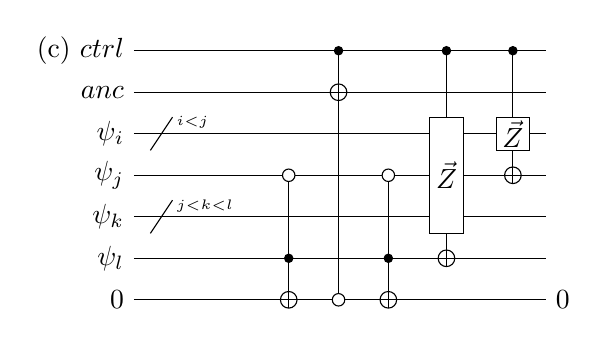
\begin{tikzpicture}[scale=1.000000,x=1pt,y=1pt]
\filldraw[color=white] (0.000000, -7.500000) rectangle (149.000000, 97.500000);
% Drawing wires
% Line 1: ctrl W \text{(c) }ctrl
\draw[color=black] (0.000000,90.000000) -- (149.000000,90.000000);
\draw[color=black] (0.000000,90.000000) node[left] {$\text{(c) }ctrl$};
% Line 2: anc W anc
\draw[color=black] (0.000000,75.000000) -- (149.000000,75.000000);
\draw[color=black] (0.000000,75.000000) node[left] {$anc$};
% Line 3: i W \psi_i
\draw[color=black] (0.000000,60.000000) -- (149.000000,60.000000);
\draw[color=black] (0.000000,60.000000) node[left] {$\psi_i$};
% Line 4: j W \psi_j
\draw[color=black] (0.000000,45.000000) -- (149.000000,45.000000);
\draw[color=black] (0.000000,45.000000) node[left] {$\psi_j$};
% Line 5: k W \psi_k
\draw[color=black] (0.000000,30.000000) -- (149.000000,30.000000);
\draw[color=black] (0.000000,30.000000) node[left] {$\psi_k$};
% Line 6: l W \psi_l
\draw[color=black] (0.000000,15.000000) -- (149.000000,15.000000);
\draw[color=black] (0.000000,15.000000) node[left] {$\psi_l$};
% Line 7: clean0 W 0 0
\draw[color=black] (0.000000,0.000000) -- (149.000000,0.000000);
\draw[color=black] (0.000000,0.000000) node[left] {$0$};
% Done with wires; drawing gates
% Line 9: i / ^{i<j}
\draw (6.000000, 54.000000) -- (14.000000, 66.000000);
\draw (12.000000, 63.000000) node[right] {$\scriptstyle{^{i<j}}$};
% Line 10: k / ^{j<k<l}
\draw (6.000000, 24.000000) -- (14.000000, 36.000000);
\draw (12.000000, 33.000000) node[right] {$\scriptstyle{^{j<k<l}}$};
% Line 11: ctrl anc i j k l clean0 LABEL
% Line 13: -j l +clean0
\draw (56.000000,45.000000) -- (56.000000,0.000000);
\draw[fill=white] (56.000000, 45.000000) circle(2.250000pt);
\filldraw (56.000000, 15.000000) circle(1.500000pt);
\begin{scope}
\draw[fill=white] (56.000000, 0.000000) circle(3.000000pt);
\clip (56.000000, 0.000000) circle(3.000000pt);
\draw (53.000000, 0.000000) -- (59.000000, 0.000000);
\draw (56.000000, -3.000000) -- (56.000000, 3.000000);
\end{scope}
% Line 14: ctrl +anc -clean0
\draw (74.000000,90.000000) -- (74.000000,0.000000);
\filldraw (74.000000, 90.000000) circle(1.500000pt);
\begin{scope}
\draw[fill=white] (74.000000, 75.000000) circle(3.000000pt);
\clip (74.000000, 75.000000) circle(3.000000pt);
\draw (71.000000, 75.000000) -- (77.000000, 75.000000);
\draw (74.000000, 72.000000) -- (74.000000, 78.000000);
\end{scope}
\draw[fill=white] (74.000000, 0.000000) circle(2.250000pt);
% Line 15: -j l +clean0
\draw (92.000000,45.000000) -- (92.000000,0.000000);
\draw[fill=white] (92.000000, 45.000000) circle(2.250000pt);
\filldraw (92.000000, 15.000000) circle(1.500000pt);
\begin{scope}
\draw[fill=white] (92.000000, 0.000000) circle(3.000000pt);
\clip (92.000000, 0.000000) circle(3.000000pt);
\draw (89.000000, 0.000000) -- (95.000000, 0.000000);
\draw (92.000000, -3.000000) -- (92.000000, 3.000000);
\end{scope}
% Line 17: i j k G $\vec{Z}$ +l ctrl
\draw (113.000000,90.000000) -- (113.000000,15.000000);
\begin{scope}
\draw[fill=white] (113.000000, 45.000000) +(-45.000000:8.485281pt and 29.698485pt) -- +(45.000000:8.485281pt and 29.698485pt) -- +(135.000000:8.485281pt and 29.698485pt) -- +(225.000000:8.485281pt and 29.698485pt) -- cycle;
\clip (113.000000, 45.000000) +(-45.000000:8.485281pt and 29.698485pt) -- +(45.000000:8.485281pt and 29.698485pt) -- +(135.000000:8.485281pt and 29.698485pt) -- +(225.000000:8.485281pt and 29.698485pt) -- cycle;
\draw (113.000000, 45.000000) node {$\vec{Z}$};
\end{scope}
\begin{scope}
\draw[fill=white] (113.000000, 15.000000) circle(3.000000pt);
\clip (113.000000, 15.000000) circle(3.000000pt);
\draw (110.000000, 15.000000) -- (116.000000, 15.000000);
\draw (113.000000, 12.000000) -- (113.000000, 18.000000);
\end{scope}
\filldraw (113.000000, 90.000000) circle(1.500000pt);
% Line 18: i G $\vec{Z}$ +j ctrl
\draw (137.000000,90.000000) -- (137.000000,45.000000);
\begin{scope}
\draw[fill=white] (137.000000, 60.000000) +(-45.000000:8.485281pt and 8.485281pt) -- +(45.000000:8.485281pt and 8.485281pt) -- +(135.000000:8.485281pt and 8.485281pt) -- +(225.000000:8.485281pt and 8.485281pt) -- cycle;
\clip (137.000000, 60.000000) +(-45.000000:8.485281pt and 8.485281pt) -- +(45.000000:8.485281pt and 8.485281pt) -- +(135.000000:8.485281pt and 8.485281pt) -- +(225.000000:8.485281pt and 8.485281pt) -- cycle;
\draw (137.000000, 60.000000) node {$\vec{Z}$};
\end{scope}
\begin{scope}
\draw[fill=white] (137.000000, 45.000000) circle(3.000000pt);
\clip (137.000000, 45.000000) circle(3.000000pt);
\draw (134.000000, 45.000000) -- (140.000000, 45.000000);
\draw (137.000000, 42.000000) -- (137.000000, 48.000000);
\end{scope}
\filldraw (137.000000, 90.000000) circle(1.500000pt);
% Done with gates; drawing ending labels
\draw[color=black] (149.000000,0.000000) node[right] {$0$};
% Done with ending labels; drawing cut lines and comments
% Done with comments
\end{tikzpicture}

        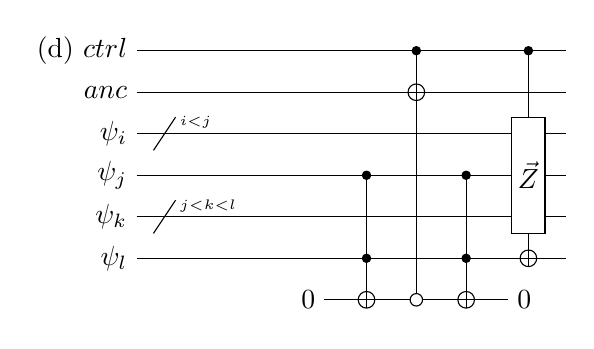
\begin{tikzpicture}[scale=1.000000,x=1pt,y=1pt]
\filldraw[color=white] (0.000000, -7.500000) rectangle (155.000000, 97.500000);
% Drawing wires
% Line 1: ctrl W \text{(d) }ctrl
\draw[color=black] (0.000000,90.000000) -- (155.000000,90.000000);
\draw[color=black] (0.000000,90.000000) node[left] {$\text{(d) }ctrl$};
% Line 2: anc W anc
\draw[color=black] (0.000000,75.000000) -- (155.000000,75.000000);
\draw[color=black] (0.000000,75.000000) node[left] {$anc$};
% Line 3: i W \psi_i
\draw[color=black] (0.000000,60.000000) -- (155.000000,60.000000);
\draw[color=black] (0.000000,60.000000) node[left] {$\psi_i$};
% Line 4: j W \psi_j
\draw[color=black] (0.000000,45.000000) -- (155.000000,45.000000);
\draw[color=black] (0.000000,45.000000) node[left] {$\psi_j$};
% Line 5: k W \psi_k
\draw[color=black] (0.000000,30.000000) -- (155.000000,30.000000);
\draw[color=black] (0.000000,30.000000) node[left] {$\psi_k$};
% Line 6: l W \psi_l
\draw[color=black] (0.000000,15.000000) -- (155.000000,15.000000);
\draw[color=black] (0.000000,15.000000) node[left] {$\psi_l$};
% Line 7: clean0 W 0 0
\draw[color=black] (60.500000,0.000000) -- (141.500000,0.000000);
% Done with wires; drawing gates
% Line 9: i / ^{i<j}
\draw (6.000000, 54.000000) -- (14.000000, 66.000000);
\draw (12.000000, 63.000000) node[right] {$\scriptstyle{^{i<j}}$};
% Line 10: k / ^{j<k<l}
\draw (6.000000, 24.000000) -- (14.000000, 36.000000);
\draw (12.000000, 33.000000) node[right] {$\scriptstyle{^{j<k<l}}$};
% Line 11: ctrl anc i j k l clean0 LABEL
% Line 13: clean0 START
\draw[color=black] (68.000000,0.000000) node[fill=white,left,minimum height=15.000000pt,minimum width=15.000000pt,inner sep=0pt] {\phantom{$0$}};
\draw[color=black] (68.000000,0.000000) node[left] {$0$};
% Line 14: j l +clean0
\draw (83.000000,45.000000) -- (83.000000,0.000000);
\filldraw (83.000000, 45.000000) circle(1.500000pt);
\filldraw (83.000000, 15.000000) circle(1.500000pt);
\begin{scope}
\draw[fill=white] (83.000000, 0.000000) circle(3.000000pt);
\clip (83.000000, 0.000000) circle(3.000000pt);
\draw (80.000000, 0.000000) -- (86.000000, 0.000000);
\draw (83.000000, -3.000000) -- (83.000000, 3.000000);
\end{scope}
% Line 15: ctrl +anc -clean0
\draw (101.000000,90.000000) -- (101.000000,0.000000);
\filldraw (101.000000, 90.000000) circle(1.500000pt);
\begin{scope}
\draw[fill=white] (101.000000, 75.000000) circle(3.000000pt);
\clip (101.000000, 75.000000) circle(3.000000pt);
\draw (98.000000, 75.000000) -- (104.000000, 75.000000);
\draw (101.000000, 72.000000) -- (101.000000, 78.000000);
\end{scope}
\draw[fill=white] (101.000000, 0.000000) circle(2.250000pt);
% Line 16: j l +clean0
\draw (119.000000,45.000000) -- (119.000000,0.000000);
\filldraw (119.000000, 45.000000) circle(1.500000pt);
\filldraw (119.000000, 15.000000) circle(1.500000pt);
\begin{scope}
\draw[fill=white] (119.000000, 0.000000) circle(3.000000pt);
\clip (119.000000, 0.000000) circle(3.000000pt);
\draw (116.000000, 0.000000) -- (122.000000, 0.000000);
\draw (119.000000, -3.000000) -- (119.000000, 3.000000);
\end{scope}
% Line 17: clean0 END
\draw[color=black] (134.000000,0.000000) node[fill=white,right,minimum height=15.000000pt,minimum width=15.000000pt,inner sep=0pt] {\phantom{$0$}};
\draw[color=black] (134.000000,0.000000) node[right] {$0$};
% Line 19: i j k G $\vec{Z}$ +l ctrl
\draw (141.500000,90.000000) -- (141.500000,15.000000);
\begin{scope}
\draw[fill=white] (141.500000, 45.000000) +(-45.000000:8.485281pt and 29.698485pt) -- +(45.000000:8.485281pt and 29.698485pt) -- +(135.000000:8.485281pt and 29.698485pt) -- +(225.000000:8.485281pt and 29.698485pt) -- cycle;
\clip (141.500000, 45.000000) +(-45.000000:8.485281pt and 29.698485pt) -- +(45.000000:8.485281pt and 29.698485pt) -- +(135.000000:8.485281pt and 29.698485pt) -- +(225.000000:8.485281pt and 29.698485pt) -- cycle;
\draw (141.500000, 45.000000) node {$\vec{Z}$};
\end{scope}
\begin{scope}
\draw[fill=white] (141.500000, 15.000000) circle(3.000000pt);
\clip (141.500000, 15.000000) circle(3.000000pt);
\draw (138.500000, 15.000000) -- (144.500000, 15.000000);
\draw (141.500000, 12.000000) -- (141.500000, 18.000000);
\end{scope}
\filldraw (141.500000, 90.000000) circle(1.500000pt);
% Done with gates; drawing ending labels
% Done with ending labels; drawing cut lines and comments
% Done with comments
\end{tikzpicture}

    }
    \caption{
        \textbf{Block-Encoding Products of Fermionic Ladder Operators}
        In subfigure a, a block-encoding for the fermionic number operator acting on the $j^\text{th}$ mode is given.
        In subfigure b, a block-encoding for the product of two fermionic number operators acting on the $j^\text{th}$ and $l^\text{th}$ modes is given.
        In subfigure c, a block-encoding for the operator $b_j^\dagger b_l$ with $i \neq l$ is given.
        In subfigure d, a block-encoding for the operator $b_j^\dagger b_j b_l$ with $i \neq l$ is given.
    }
    \label{fig:fermionic-products-be}
\end{figure}

As a simple example where we can produce a more efficient construction, consider the fermionic number operator: $b_j^\dagger b_j$.
Note the behavior of the conjoined operator on an arbitrary quantum state:
\begin{equation}
    \begin{split}
        b_j^\dagger b_j \ket{\psi_{b_j}} = \begin{cases} 
            \ket{1} & \text{when $\ket{\psi_{b_j}}$ is $\ket{1}$} \\
            0 & \text{when $\ket{\psi_{b_j}}$ is $\ket{0}$} \\
                                        \end{cases}
    \end{split}
\end{equation}
If the $j^\text{th}$ mode is unoccupied, the state will be zeroed-out.
If the $j^\text{th}$ mode is occupied, then the state is left unchanged.
We can describe this action using the circuit shown in subfigure \ref{fig:fermionic-products-be}a.
The Toffoli gate flips the block-encoding ancilla outside the subspace if the control is on and the $j^\text{th}$ mode is unoccupied.
Otherwise, the state of the system and the block-encoding ancilla are left unchanged.
Block-encoding this operator as the product of the block-encodings for $b_j^\dagger$ and $b_j$ would require $2$ Toffoli gates and $2$ block-encoding ancillae.
The construction given here requires only one Toffoli gate and one block-encoding ancilla.

For a more general product of two fermionic ladder operators, a block-encoding circuit for the operator $b_j^\dagger b_l$ is given in subfigure \ref{fig:fermionic-products-be}c.
For this operator, we can infer that the state will be zeroed-out \textit{unless} both the $j^\text{th}$ mode is unoccupied and the $l^\text{th}$ mode is occupied.
The temporary logical-AND of these two conditions is stored in a clean ancilla.
If the control qubit is on and these two conditions on the system are not true, then the block-encoding ancilla is flipped outside of the encoded subspace.
After the state of the block-encoding ancilla is determined, the system is updated by applying the two operators onto the system in order: $b_l$ then $b_j^\dagger$.
These operators are applied using similar operators of the form $\vec{Z}X$ which applies the appropriate sign flip based on the occupation of the preceeding modes and updates the occupation of the fermionic mode.
This block-encoding circuit has an optimal rescaling factor ($\lambda = 1$), requires one block-encoding ancilla, and uses two Toffoli gates.


This construction can be generalized to an arbitrary product of ladder operators.
Let $B$ represent the number of active modes in a term where we define an active mode as a mode that has a ladder operator applied to it.
For example, the term $b_i b_j^\dagger b_k b_l^\dagger b_l$ has $4$ active modes.
Each active mode will contribute a new control on the state of the mode.
For a general product of fermionic ladder operators, a block-encoding circuit of this form will have an optimal rescaling factor ($\lambda = 1$), require only one block-encoding ancilla, and use $B$ Toffoli gates.
The count of $B$ Toffoli gates assumes that each $B$-controlled NOT gate is decomposed into a series of $B-1$ Toffoli gates as described in Appendix \ref{sec:elbows}.

\ws{
A natural question to ask is how do these constructions compare with using an LCU block-encoding after applying the Jordan-Wigner transformation \cite{}?
The Jordan-Wigner transformation maps each fermionic ladder operator (or number operator) to a sum of two Pauli operators.
For an arbitrary product of fermionic ladder operators, expanding these linear combinations results in $2^{B}$ Paulis.
The number of non-Clifford gates for LCU scales linearly with the number of operators and hence would scale exponentially with $B$ under this construction.
Alternatively, one could construct LCU block-encodings for each of the ladder operators in a term by applying the Jordan-Wigner transformation to each ladder operator (or number operator) independently.
The product of these block-encodings would then give a block-encoding of the term.
For each ladder operator (or number operator), an LCU block-encoding would require one Toffoli gate and one ancilla qubit.
A block-encoding of the whole term using this construction would then require $B$ Toffoli gates and $B$ block-encoding ancillae.
}

\subsection{Linear Combinations of Fermionic Ladder Operators}


As discussed in subsection \ref{subsec:be-products}, a block-encoding for a linear combination of operators can be constructed using the LCO framework (Theorem \ref{th:lco}).
In this subsection, we show how to construct block-encodings of linear combinations of products of fermionic ladder operators that use fewer quantum resources than are required by an LCO construction.
In particular, we give a generalizable construction for a product of fermionic ladder operators plus its hermitian conjugate.
However, we note that the strategies we present here are not restricted only to these linear combinations.

\begin{figure}
    \mbox{
        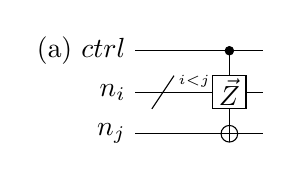
\begin{tikzpicture}[scale=1.000000,x=1pt,y=1pt]
\filldraw[color=white] (0.000000, -7.500000) rectangle (46.000000, 37.500000);
% Drawing wires
% Line 1: a W \text{(a) }ctrl
\draw[color=black] (0.000000,30.000000) -- (46.000000,30.000000);
\draw[color=black] (0.000000,30.000000) node[left] {$\text{(a) }ctrl$};
% Line 2: b W n_i
\draw[color=black] (0.000000,15.000000) -- (46.000000,15.000000);
\draw[color=black] (0.000000,15.000000) node[left] {$n_i$};
% Line 3: c W n_j
\draw[color=black] (0.000000,0.000000) -- (46.000000,0.000000);
\draw[color=black] (0.000000,0.000000) node[left] {$n_j$};
% Done with wires; drawing gates
% Line 5: b / ^{i<j}
\draw (6.000000, 9.000000) -- (14.000000, 21.000000);
\draw (12.000000, 18.000000) node[right] {$\scriptstyle{^{i<j}}$};
% Line 6: a b c LABEL width=-10
% Line 7: b G $\vec{Z}$ a +c
\draw (34.000000,30.000000) -- (34.000000,0.000000);
\begin{scope}
\draw[fill=white] (34.000000, 15.000000) +(-45.000000:8.485281pt and 8.485281pt) -- +(45.000000:8.485281pt and 8.485281pt) -- +(135.000000:8.485281pt and 8.485281pt) -- +(225.000000:8.485281pt and 8.485281pt) -- cycle;
\clip (34.000000, 15.000000) +(-45.000000:8.485281pt and 8.485281pt) -- +(45.000000:8.485281pt and 8.485281pt) -- +(135.000000:8.485281pt and 8.485281pt) -- +(225.000000:8.485281pt and 8.485281pt) -- cycle;
\draw (34.000000, 15.000000) node {$\vec{Z}$};
\end{scope}
\filldraw (34.000000, 30.000000) circle(1.500000pt);
\begin{scope}
\draw[fill=white] (34.000000, 0.000000) circle(3.000000pt);
\clip (34.000000, 0.000000) circle(3.000000pt);
\draw (31.000000, 0.000000) -- (37.000000, 0.000000);
\draw (34.000000, -3.000000) -- (34.000000, 3.000000);
\end{scope}
% Done with gates; drawing ending labels
% Done with ending labels; drawing cut lines and comments
% Done with comments
\end{tikzpicture}

        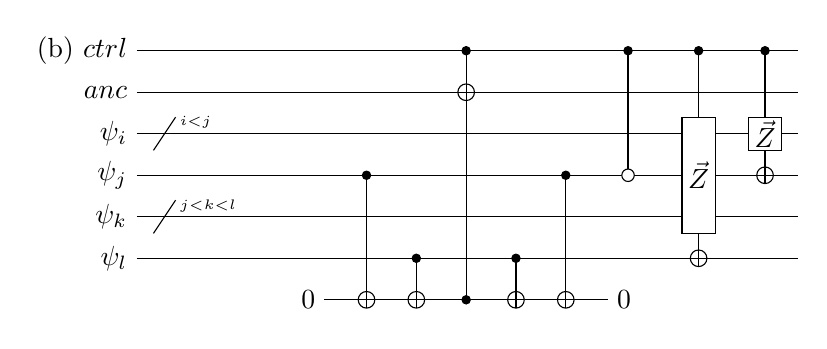
\begin{tikzpicture}[scale=1.000000,x=1pt,y=1pt]
\filldraw[color=white] (0.000000, -7.500000) rectangle (239.000000, 97.500000);
% Drawing wires
% Line 1: c W \text{(b) }ctrl
\draw[color=black] (0.000000,90.000000) -- (239.000000,90.000000);
\draw[color=black] (0.000000,90.000000) node[left] {$\text{(b) }ctrl$};
% Line 2: a W anc
\draw[color=black] (0.000000,75.000000) -- (239.000000,75.000000);
\draw[color=black] (0.000000,75.000000) node[left] {$anc$};
% Line 3: i W \psi_i
\draw[color=black] (0.000000,60.000000) -- (239.000000,60.000000);
\draw[color=black] (0.000000,60.000000) node[left] {$\psi_i$};
% Line 4: j W \psi_j
\draw[color=black] (0.000000,45.000000) -- (239.000000,45.000000);
\draw[color=black] (0.000000,45.000000) node[left] {$\psi_j$};
% Line 5: k W \psi_k
\draw[color=black] (0.000000,30.000000) -- (239.000000,30.000000);
\draw[color=black] (0.000000,30.000000) node[left] {$\psi_k$};
% Line 6: l W \psi_l
\draw[color=black] (0.000000,15.000000) -- (239.000000,15.000000);
\draw[color=black] (0.000000,15.000000) node[left] {$\psi_l$};
% Line 7: c0 W 0 0
\draw[color=black] (60.500000,0.000000) -- (177.500000,0.000000);
% Done with wires; drawing gates
% Line 9: i / ^{i<j}
\draw (6.000000, 54.000000) -- (14.000000, 66.000000);
\draw (12.000000, 63.000000) node[right] {$\scriptstyle{^{i<j}}$};
% Line 10: k / ^{j<k<l}
\draw (6.000000, 24.000000) -- (14.000000, 36.000000);
\draw (12.000000, 33.000000) node[right] {$\scriptstyle{^{j<k<l}}$};
% Line 11: c a i j k l c0 LABEL
% Line 12: c0 START
\draw[color=black] (68.000000,0.000000) node[fill=white,left,minimum height=15.000000pt,minimum width=15.000000pt,inner sep=0pt] {\phantom{$0$}};
\draw[color=black] (68.000000,0.000000) node[left] {$0$};
% Line 13: j +c0
\draw (83.000000,45.000000) -- (83.000000,0.000000);
\filldraw (83.000000, 45.000000) circle(1.500000pt);
\begin{scope}
\draw[fill=white] (83.000000, 0.000000) circle(3.000000pt);
\clip (83.000000, 0.000000) circle(3.000000pt);
\draw (80.000000, 0.000000) -- (86.000000, 0.000000);
\draw (83.000000, -3.000000) -- (83.000000, 3.000000);
\end{scope}
% Line 14: l +c0
\draw (101.000000,15.000000) -- (101.000000,0.000000);
\filldraw (101.000000, 15.000000) circle(1.500000pt);
\begin{scope}
\draw[fill=white] (101.000000, 0.000000) circle(3.000000pt);
\clip (101.000000, 0.000000) circle(3.000000pt);
\draw (98.000000, 0.000000) -- (104.000000, 0.000000);
\draw (101.000000, -3.000000) -- (101.000000, 3.000000);
\end{scope}
% Line 15: c c0 +a
\draw (119.000000,90.000000) -- (119.000000,0.000000);
\filldraw (119.000000, 90.000000) circle(1.500000pt);
\filldraw (119.000000, 0.000000) circle(1.500000pt);
\begin{scope}
\draw[fill=white] (119.000000, 75.000000) circle(3.000000pt);
\clip (119.000000, 75.000000) circle(3.000000pt);
\draw (116.000000, 75.000000) -- (122.000000, 75.000000);
\draw (119.000000, 72.000000) -- (119.000000, 78.000000);
\end{scope}
% Line 16: l +c0
\draw (137.000000,15.000000) -- (137.000000,0.000000);
\filldraw (137.000000, 15.000000) circle(1.500000pt);
\begin{scope}
\draw[fill=white] (137.000000, 0.000000) circle(3.000000pt);
\clip (137.000000, 0.000000) circle(3.000000pt);
\draw (134.000000, 0.000000) -- (140.000000, 0.000000);
\draw (137.000000, -3.000000) -- (137.000000, 3.000000);
\end{scope}
% Line 17: j +c0
\draw (155.000000,45.000000) -- (155.000000,0.000000);
\filldraw (155.000000, 45.000000) circle(1.500000pt);
\begin{scope}
\draw[fill=white] (155.000000, 0.000000) circle(3.000000pt);
\clip (155.000000, 0.000000) circle(3.000000pt);
\draw (152.000000, 0.000000) -- (158.000000, 0.000000);
\draw (155.000000, -3.000000) -- (155.000000, 3.000000);
\end{scope}
% Line 18: c0 END
\draw[color=black] (170.000000,0.000000) node[fill=white,right,minimum height=15.000000pt,minimum width=15.000000pt,inner sep=0pt] {\phantom{$0$}};
\draw[color=black] (170.000000,0.000000) node[right] {$0$};
% Line 19: c -j
\draw (177.500000,90.000000) -- (177.500000,45.000000);
\filldraw (177.500000, 90.000000) circle(1.500000pt);
\draw[fill=white] (177.500000, 45.000000) circle(2.250000pt);
% Line 21: i j k G $\vec{Z}$ c +l
\draw (203.000000,90.000000) -- (203.000000,15.000000);
\begin{scope}
\draw[fill=white] (203.000000, 45.000000) +(-45.000000:8.485281pt and 29.698485pt) -- +(45.000000:8.485281pt and 29.698485pt) -- +(135.000000:8.485281pt and 29.698485pt) -- +(225.000000:8.485281pt and 29.698485pt) -- cycle;
\clip (203.000000, 45.000000) +(-45.000000:8.485281pt and 29.698485pt) -- +(45.000000:8.485281pt and 29.698485pt) -- +(135.000000:8.485281pt and 29.698485pt) -- +(225.000000:8.485281pt and 29.698485pt) -- cycle;
\draw (203.000000, 45.000000) node {$\vec{Z}$};
\end{scope}
\filldraw (203.000000, 90.000000) circle(1.500000pt);
\begin{scope}
\draw[fill=white] (203.000000, 15.000000) circle(3.000000pt);
\clip (203.000000, 15.000000) circle(3.000000pt);
\draw (200.000000, 15.000000) -- (206.000000, 15.000000);
\draw (203.000000, 12.000000) -- (203.000000, 18.000000);
\end{scope}
% Line 22: i G $\vec{Z}$ c +j
\draw (227.000000,90.000000) -- (227.000000,45.000000);
\begin{scope}
\draw[fill=white] (227.000000, 60.000000) +(-45.000000:8.485281pt and 8.485281pt) -- +(45.000000:8.485281pt and 8.485281pt) -- +(135.000000:8.485281pt and 8.485281pt) -- +(225.000000:8.485281pt and 8.485281pt) -- cycle;
\clip (227.000000, 60.000000) +(-45.000000:8.485281pt and 8.485281pt) -- +(45.000000:8.485281pt and 8.485281pt) -- +(135.000000:8.485281pt and 8.485281pt) -- +(225.000000:8.485281pt and 8.485281pt) -- cycle;
\draw (227.000000, 60.000000) node {$\vec{Z}$};
\end{scope}
\filldraw (227.000000, 90.000000) circle(1.500000pt);
\begin{scope}
\draw[fill=white] (227.000000, 45.000000) circle(3.000000pt);
\clip (227.000000, 45.000000) circle(3.000000pt);
\draw (224.000000, 45.000000) -- (230.000000, 45.000000);
\draw (227.000000, 42.000000) -- (227.000000, 48.000000);
\end{scope}
% Done with gates; drawing ending labels
% Done with ending labels; drawing cut lines and comments
% Done with comments
\end{tikzpicture}

    }
    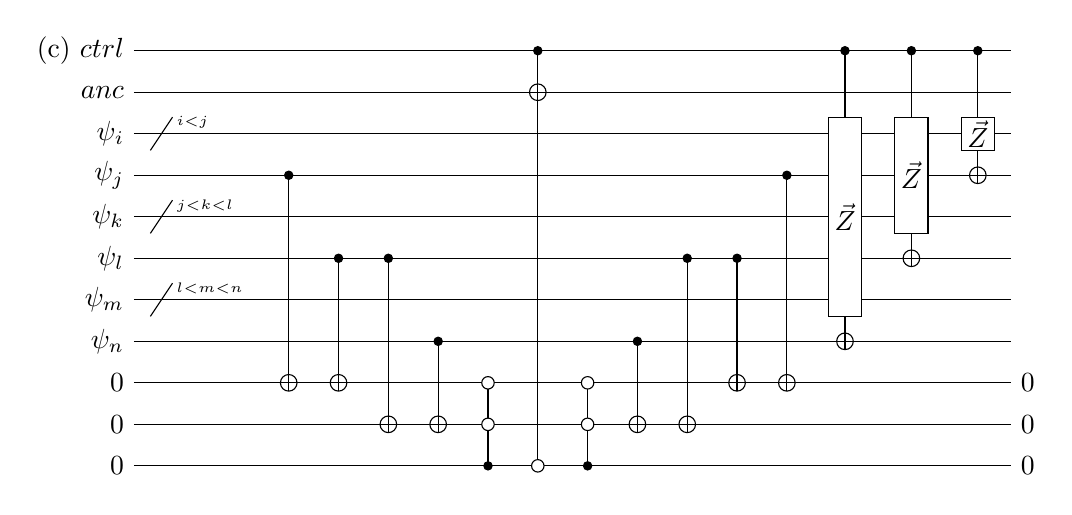
\begin{tikzpicture}[scale=1.000000,x=1pt,y=1pt]
\filldraw[color=white] (0.000000, -7.500000) rectangle (317.000000, 157.500000);
% Drawing wires
% Line 1: ctrl W \text{(c) }ctrl
\draw[color=black] (0.000000,150.000000) -- (317.000000,150.000000);
\draw[color=black] (0.000000,150.000000) node[left] {$\text{(c) }ctrl$};
% Line 2: anc W anc
\draw[color=black] (0.000000,135.000000) -- (317.000000,135.000000);
\draw[color=black] (0.000000,135.000000) node[left] {$anc$};
% Line 3: i W \psi_i
\draw[color=black] (0.000000,120.000000) -- (317.000000,120.000000);
\draw[color=black] (0.000000,120.000000) node[left] {$\psi_i$};
% Line 4: j W \psi_j
\draw[color=black] (0.000000,105.000000) -- (317.000000,105.000000);
\draw[color=black] (0.000000,105.000000) node[left] {$\psi_j$};
% Line 5: k W \psi_k
\draw[color=black] (0.000000,90.000000) -- (317.000000,90.000000);
\draw[color=black] (0.000000,90.000000) node[left] {$\psi_k$};
% Line 6: l W \psi_l
\draw[color=black] (0.000000,75.000000) -- (317.000000,75.000000);
\draw[color=black] (0.000000,75.000000) node[left] {$\psi_l$};
% Line 7: m W \psi_m
\draw[color=black] (0.000000,60.000000) -- (317.000000,60.000000);
\draw[color=black] (0.000000,60.000000) node[left] {$\psi_m$};
% Line 8: n W \psi_n
\draw[color=black] (0.000000,45.000000) -- (317.000000,45.000000);
\draw[color=black] (0.000000,45.000000) node[left] {$\psi_n$};
% Line 9: clean0 W 0 0
\draw[color=black] (0.000000,30.000000) -- (317.000000,30.000000);
\draw[color=black] (0.000000,30.000000) node[left] {$0$};
% Line 10: clean1 W 0 0
\draw[color=black] (0.000000,15.000000) -- (317.000000,15.000000);
\draw[color=black] (0.000000,15.000000) node[left] {$0$};
% Line 11: clean2 W 0 0
\draw[color=black] (0.000000,0.000000) -- (317.000000,0.000000);
\draw[color=black] (0.000000,0.000000) node[left] {$0$};
% Done with wires; drawing gates
% Line 13: i / ^{i<j}
\draw (6.000000, 114.000000) -- (14.000000, 126.000000);
\draw (12.000000, 123.000000) node[right] {$\scriptstyle{^{i<j}}$};
% Line 14: k / ^{j<k<l}
\draw (6.000000, 84.000000) -- (14.000000, 96.000000);
\draw (12.000000, 93.000000) node[right] {$\scriptstyle{^{j<k<l}}$};
% Line 15: m / ^{l<m<n}
\draw (6.000000, 54.000000) -- (14.000000, 66.000000);
\draw (12.000000, 63.000000) node[right] {$\scriptstyle{^{l<m<n}}$};
% Line 16: ctrl anc i j k l m n clean0 LABEL
% Line 17: j +clean0
\draw (56.000000,105.000000) -- (56.000000,30.000000);
\filldraw (56.000000, 105.000000) circle(1.500000pt);
\begin{scope}
\draw[fill=white] (56.000000, 30.000000) circle(3.000000pt);
\clip (56.000000, 30.000000) circle(3.000000pt);
\draw (53.000000, 30.000000) -- (59.000000, 30.000000);
\draw (56.000000, 27.000000) -- (56.000000, 33.000000);
\end{scope}
% Line 18: l +clean0
\draw (74.000000,75.000000) -- (74.000000,30.000000);
\filldraw (74.000000, 75.000000) circle(1.500000pt);
\begin{scope}
\draw[fill=white] (74.000000, 30.000000) circle(3.000000pt);
\clip (74.000000, 30.000000) circle(3.000000pt);
\draw (71.000000, 30.000000) -- (77.000000, 30.000000);
\draw (74.000000, 27.000000) -- (74.000000, 33.000000);
\end{scope}
% Line 19: l +clean1
\draw (92.000000,75.000000) -- (92.000000,15.000000);
\filldraw (92.000000, 75.000000) circle(1.500000pt);
\begin{scope}
\draw[fill=white] (92.000000, 15.000000) circle(3.000000pt);
\clip (92.000000, 15.000000) circle(3.000000pt);
\draw (89.000000, 15.000000) -- (95.000000, 15.000000);
\draw (92.000000, 12.000000) -- (92.000000, 18.000000);
\end{scope}
% Line 20: n +clean1
\draw (110.000000,45.000000) -- (110.000000,15.000000);
\filldraw (110.000000, 45.000000) circle(1.500000pt);
\begin{scope}
\draw[fill=white] (110.000000, 15.000000) circle(3.000000pt);
\clip (110.000000, 15.000000) circle(3.000000pt);
\draw (107.000000, 15.000000) -- (113.000000, 15.000000);
\draw (110.000000, 12.000000) -- (110.000000, 18.000000);
\end{scope}
% Line 21: -clean0 -clean1 clean2
\draw (128.000000,30.000000) -- (128.000000,0.000000);
\draw[fill=white] (128.000000, 30.000000) circle(2.250000pt);
\draw[fill=white] (128.000000, 15.000000) circle(2.250000pt);
\filldraw (128.000000, 0.000000) circle(1.500000pt);
% Line 22: ctrl -clean2 +anc
\draw (146.000000,150.000000) -- (146.000000,0.000000);
\filldraw (146.000000, 150.000000) circle(1.500000pt);
\draw[fill=white] (146.000000, 0.000000) circle(2.250000pt);
\begin{scope}
\draw[fill=white] (146.000000, 135.000000) circle(3.000000pt);
\clip (146.000000, 135.000000) circle(3.000000pt);
\draw (143.000000, 135.000000) -- (149.000000, 135.000000);
\draw (146.000000, 132.000000) -- (146.000000, 138.000000);
\end{scope}
% Line 23: -clean0 -clean1 clean2
\draw (164.000000,30.000000) -- (164.000000,0.000000);
\draw[fill=white] (164.000000, 30.000000) circle(2.250000pt);
\draw[fill=white] (164.000000, 15.000000) circle(2.250000pt);
\filldraw (164.000000, 0.000000) circle(1.500000pt);
% Line 24: n +clean1
\draw (182.000000,45.000000) -- (182.000000,15.000000);
\filldraw (182.000000, 45.000000) circle(1.500000pt);
\begin{scope}
\draw[fill=white] (182.000000, 15.000000) circle(3.000000pt);
\clip (182.000000, 15.000000) circle(3.000000pt);
\draw (179.000000, 15.000000) -- (185.000000, 15.000000);
\draw (182.000000, 12.000000) -- (182.000000, 18.000000);
\end{scope}
% Line 25: l +clean1
\draw (200.000000,75.000000) -- (200.000000,15.000000);
\filldraw (200.000000, 75.000000) circle(1.500000pt);
\begin{scope}
\draw[fill=white] (200.000000, 15.000000) circle(3.000000pt);
\clip (200.000000, 15.000000) circle(3.000000pt);
\draw (197.000000, 15.000000) -- (203.000000, 15.000000);
\draw (200.000000, 12.000000) -- (200.000000, 18.000000);
\end{scope}
% Line 26: l +clean0
\draw (218.000000,75.000000) -- (218.000000,30.000000);
\filldraw (218.000000, 75.000000) circle(1.500000pt);
\begin{scope}
\draw[fill=white] (218.000000, 30.000000) circle(3.000000pt);
\clip (218.000000, 30.000000) circle(3.000000pt);
\draw (215.000000, 30.000000) -- (221.000000, 30.000000);
\draw (218.000000, 27.000000) -- (218.000000, 33.000000);
\end{scope}
% Line 27: j +clean0
\draw (236.000000,105.000000) -- (236.000000,30.000000);
\filldraw (236.000000, 105.000000) circle(1.500000pt);
\begin{scope}
\draw[fill=white] (236.000000, 30.000000) circle(3.000000pt);
\clip (236.000000, 30.000000) circle(3.000000pt);
\draw (233.000000, 30.000000) -- (239.000000, 30.000000);
\draw (236.000000, 27.000000) -- (236.000000, 33.000000);
\end{scope}
% Line 29: i j k l m G $\vec{Z}$ ctrl +n
\draw (257.000000,150.000000) -- (257.000000,45.000000);
\begin{scope}
\draw[fill=white] (257.000000, 90.000000) +(-45.000000:8.485281pt and 50.911688pt) -- +(45.000000:8.485281pt and 50.911688pt) -- +(135.000000:8.485281pt and 50.911688pt) -- +(225.000000:8.485281pt and 50.911688pt) -- cycle;
\clip (257.000000, 90.000000) +(-45.000000:8.485281pt and 50.911688pt) -- +(45.000000:8.485281pt and 50.911688pt) -- +(135.000000:8.485281pt and 50.911688pt) -- +(225.000000:8.485281pt and 50.911688pt) -- cycle;
\draw (257.000000, 90.000000) node {$\vec{Z}$};
\end{scope}
\filldraw (257.000000, 150.000000) circle(1.500000pt);
\begin{scope}
\draw[fill=white] (257.000000, 45.000000) circle(3.000000pt);
\clip (257.000000, 45.000000) circle(3.000000pt);
\draw (254.000000, 45.000000) -- (260.000000, 45.000000);
\draw (257.000000, 42.000000) -- (257.000000, 48.000000);
\end{scope}
% Line 30: i j k G $\vec{Z}$ ctrl +l
\draw (281.000000,150.000000) -- (281.000000,75.000000);
\begin{scope}
\draw[fill=white] (281.000000, 105.000000) +(-45.000000:8.485281pt and 29.698485pt) -- +(45.000000:8.485281pt and 29.698485pt) -- +(135.000000:8.485281pt and 29.698485pt) -- +(225.000000:8.485281pt and 29.698485pt) -- cycle;
\clip (281.000000, 105.000000) +(-45.000000:8.485281pt and 29.698485pt) -- +(45.000000:8.485281pt and 29.698485pt) -- +(135.000000:8.485281pt and 29.698485pt) -- +(225.000000:8.485281pt and 29.698485pt) -- cycle;
\draw (281.000000, 105.000000) node {$\vec{Z}$};
\end{scope}
\filldraw (281.000000, 150.000000) circle(1.500000pt);
\begin{scope}
\draw[fill=white] (281.000000, 75.000000) circle(3.000000pt);
\clip (281.000000, 75.000000) circle(3.000000pt);
\draw (278.000000, 75.000000) -- (284.000000, 75.000000);
\draw (281.000000, 72.000000) -- (281.000000, 78.000000);
\end{scope}
% Line 31: i G $\vec{Z}$ ctrl +j
\draw (305.000000,150.000000) -- (305.000000,105.000000);
\begin{scope}
\draw[fill=white] (305.000000, 120.000000) +(-45.000000:8.485281pt and 8.485281pt) -- +(45.000000:8.485281pt and 8.485281pt) -- +(135.000000:8.485281pt and 8.485281pt) -- +(225.000000:8.485281pt and 8.485281pt) -- cycle;
\clip (305.000000, 120.000000) +(-45.000000:8.485281pt and 8.485281pt) -- +(45.000000:8.485281pt and 8.485281pt) -- +(135.000000:8.485281pt and 8.485281pt) -- +(225.000000:8.485281pt and 8.485281pt) -- cycle;
\draw (305.000000, 120.000000) node {$\vec{Z}$};
\end{scope}
\filldraw (305.000000, 150.000000) circle(1.500000pt);
\begin{scope}
\draw[fill=white] (305.000000, 105.000000) circle(3.000000pt);
\clip (305.000000, 105.000000) circle(3.000000pt);
\draw (302.000000, 105.000000) -- (308.000000, 105.000000);
\draw (305.000000, 102.000000) -- (305.000000, 108.000000);
\end{scope}
% Done with gates; drawing ending labels
\draw[color=black] (317.000000,30.000000) node[right] {$0$};
\draw[color=black] (317.000000,15.000000) node[right] {$0$};
\draw[color=black] (317.000000,0.000000) node[right] {$0$};
% Done with ending labels; drawing cut lines and comments
% Done with comments
\end{tikzpicture}

    \caption{
        \textbf{Block-Encoding Product of Fermionic Operators Plus Hermitian Conjugate}
        In subfigure a, a block-encoding for the operator $b_j + b_j^\dagger$ is given.
        In subfigure b, a block-encoding for the operator $b_j b_l + b_l^\dagger b_j^\dagger$ is given.
        In subfigure c, a block-encoding for the operator $b_j b_l b_n + b_n^\dagger b_l^\dagger b_j^\dagger$ is given.
        For the 3-body term, the $CZ$ gate is not present since the swapping of the order of the operators results in both terms being positive: $b_j b_l b_n + b_j^\dagger b_l^\dagger b_n^\dagger$.
    }
    \label{fig:fermionic-be-lc-small}
\end{figure}


For a simple example, we begin with a linear combination of an individual fermionic ladder operator with its hermitian conjugate: $b_j^\dagger + b_j$.
Consider the action of the joined operator on the two possible occupation states of the $j^\text{th}$ fermionic mode:
\begin{equation}
    \begin{split}
        (b_j^\dagger + b_j) \ket{\psi_{b_j}} = \begin{cases} 
            \ket{1} & \text{when $\ket{\psi_{b_j}}$ is $\ket{0}$} \\
            \ket{0} & \text{when $\ket{\psi_{b_j}}$ is $\ket{1}$} \\
                                        \end{cases}
    \end{split}
\end{equation}
where the sign flip depending on the parity of the occupation of the preceeding fermionic modes is again omitted in this section for brevity.
From this perspective, it is obvious that a block-encoding for this linear combination of operators can be achieved simply using a Pauli $X$ gate on the $j^\text{th}$ mode and Pauli $Z$ gates on each fermionic mode with index $i < j$.
A circuit diagram for this block-encoding is shown in subfigure \ref{fig:fermionic-be-lc-small}a.
One might notice that this is the same construction one would arrive at using the Jordan-Wigner transformation of the above operators.
This block-encoding circuit has an optimal rescaling factor ($\lambda = 1$), requires no ancilla and no non-Clifford gates.
An LCO construction using the block-encodings for these two ladder operators individually would have a rescaling factor of $2$, would require one block-encoding ancillae, and one Toffoli gate to index between the two terms.


For a two-body fermionic operator and its hermitian conjugate ($b_j b_l + b_l^\dagger b_j^\dagger$) we arrive at a construction that differs from the Jordan-Wigner transformation.
We begin by swapping the operators in the second term using the anticommutation relations to ensure that the order is the same: $b_j b_l - b_j^\dagger b_l^\dagger$.
In the circuit, the serial order in which we apply the operators is fixed so it must be consistent for both terms.
The action of the joined operator on the possible occupation states of the $i^\text{th}$ and $j^\text{th}$ fermionic modes is given by:
\begin{equation}
    \begin{split}
        (b_j b_l - b_j^\dagger b_l^\dagger) \ket{\psi_{b_j}, \psi_{b_l}} = \begin{cases} 
            \hspace{1em}\ket{11} & \text{when $\ket{\psi_{b_j}, \psi_{b_l}}$ is $\ket{00}$} \\
            -\ket{00} & \text{when $\ket{\psi_{b_j}, \psi_{b_l}}$ is $\ket{11}$} \\
                                        \end{cases}
    \end{split}
\end{equation}
The sign flip caused by the parity of the preceeding modes will be consistent for both terms since the order at which the operators appear in each term is consistent. 
The desired action of this operator on the state is determined by the parity of the two fermionic modes.
If $\ket{a} = \ket{\psi_{b_j}} \oplus \ket{\psi_{b_l}}$, then the state will be zeroed-out by the operator \textit{unless} $\ket{a} = \ket{0}$.

In subfigure \ref{fig:fermionic-be-lc-small}b, we give a circuit diagram for block-encoding this two-body operator.
The variable $\ket{a}$ can be computed using two CNOT gates targeting a clean ancilla and controlled on the $j^\text{th}$ and $l^\text{th}$ fermionic modes.
If the control qubit is on and $\ket{a}$ is in the $\ket{0}$ state, then the block-encoding ancilla is flipped to push that branch of the wavefunction outside of the encoded subspace.
After this operation, the variable $\ket{a}$ can be uncomputed, returning this ancilla to a clean state.
Next, a $CZ$ gate that is $0$-controlled on the $j^\text{th}$ fermionic mode applies the desired sign flip onto the state corresponding to the term $- b_j^\dagger b_l^\dagger$.
Lastly, a series of $\vec{Z}X$ operators are applied to each active mode in the order at which the operators would be applied onto the quantum state (right to left).

\begin{figure}
    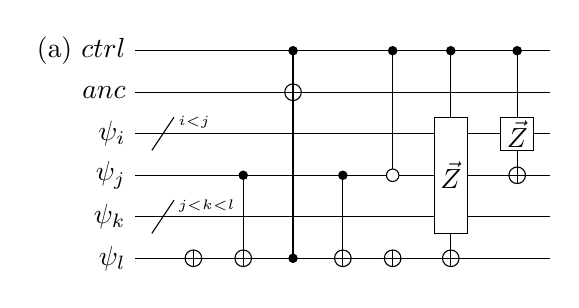
\begin{tikzpicture}[scale=1.000000,x=1pt,y=1pt]
\filldraw[color=white] (0.000000, -7.500000) rectangle (150.000000, 82.500000);
% Drawing wires
% Line 1: c W \text{(a) }ctrl
\draw[color=black] (0.000000,75.000000) -- (150.000000,75.000000);
\draw[color=black] (0.000000,75.000000) node[left] {$\text{(a) }ctrl$};
% Line 2: a W anc
\draw[color=black] (0.000000,60.000000) -- (150.000000,60.000000);
\draw[color=black] (0.000000,60.000000) node[left] {$anc$};
% Line 3: i W \psi_i
\draw[color=black] (0.000000,45.000000) -- (150.000000,45.000000);
\draw[color=black] (0.000000,45.000000) node[left] {$\psi_i$};
% Line 4: j W \psi_j
\draw[color=black] (0.000000,30.000000) -- (150.000000,30.000000);
\draw[color=black] (0.000000,30.000000) node[left] {$\psi_j$};
% Line 5: k W \psi_k
\draw[color=black] (0.000000,15.000000) -- (150.000000,15.000000);
\draw[color=black] (0.000000,15.000000) node[left] {$\psi_k$};
% Line 6: l W \psi_l
\draw[color=black] (0.000000,0.000000) -- (150.000000,0.000000);
\draw[color=black] (0.000000,0.000000) node[left] {$\psi_l$};
% Done with wires; drawing gates
% Line 8: i / ^{i<j}
\draw (6.000000, 39.000000) -- (14.000000, 51.000000);
\draw (12.000000, 48.000000) node[right] {$\scriptstyle{^{i<j}}$};
% Line 9: k / ^{j<k<l}
\draw (6.000000, 9.000000) -- (14.000000, 21.000000);
\draw (12.000000, 18.000000) node[right] {$\scriptstyle{^{j<k<l}}$};
% Line 10: c a i j k l LABEL width=-20
% Line 12: +l
\begin{scope}
\draw[fill=white] (21.000000, 0.000000) circle(3.000000pt);
\clip (21.000000, 0.000000) circle(3.000000pt);
\draw (18.000000, 0.000000) -- (24.000000, 0.000000);
\draw (21.000000, -3.000000) -- (21.000000, 3.000000);
\end{scope}
% Line 13: j +l
\draw (39.000000,30.000000) -- (39.000000,0.000000);
\filldraw (39.000000, 30.000000) circle(1.500000pt);
\begin{scope}
\draw[fill=white] (39.000000, 0.000000) circle(3.000000pt);
\clip (39.000000, 0.000000) circle(3.000000pt);
\draw (36.000000, 0.000000) -- (42.000000, 0.000000);
\draw (39.000000, -3.000000) -- (39.000000, 3.000000);
\end{scope}
% Line 14: c l +a
\draw (57.000000,75.000000) -- (57.000000,0.000000);
\filldraw (57.000000, 75.000000) circle(1.500000pt);
\filldraw (57.000000, 0.000000) circle(1.500000pt);
\begin{scope}
\draw[fill=white] (57.000000, 60.000000) circle(3.000000pt);
\clip (57.000000, 60.000000) circle(3.000000pt);
\draw (54.000000, 60.000000) -- (60.000000, 60.000000);
\draw (57.000000, 57.000000) -- (57.000000, 63.000000);
\end{scope}
% Line 15: j +l
\draw (75.000000,30.000000) -- (75.000000,0.000000);
\filldraw (75.000000, 30.000000) circle(1.500000pt);
\begin{scope}
\draw[fill=white] (75.000000, 0.000000) circle(3.000000pt);
\clip (75.000000, 0.000000) circle(3.000000pt);
\draw (72.000000, 0.000000) -- (78.000000, 0.000000);
\draw (75.000000, -3.000000) -- (75.000000, 3.000000);
\end{scope}
% Line 16: +l
\begin{scope}
\draw[fill=white] (93.000000, 0.000000) circle(3.000000pt);
\clip (93.000000, 0.000000) circle(3.000000pt);
\draw (90.000000, 0.000000) -- (96.000000, 0.000000);
\draw (93.000000, -3.000000) -- (93.000000, 3.000000);
\end{scope}
% Line 18: c -j
\draw (93.000000,75.000000) -- (93.000000,30.000000);
\filldraw (93.000000, 75.000000) circle(1.500000pt);
\draw[fill=white] (93.000000, 30.000000) circle(2.250000pt);
% Line 20: i j k G $\vec{Z}$ c +l
\draw (114.000000,75.000000) -- (114.000000,0.000000);
\begin{scope}
\draw[fill=white] (114.000000, 30.000000) +(-45.000000:8.485281pt and 29.698485pt) -- +(45.000000:8.485281pt and 29.698485pt) -- +(135.000000:8.485281pt and 29.698485pt) -- +(225.000000:8.485281pt and 29.698485pt) -- cycle;
\clip (114.000000, 30.000000) +(-45.000000:8.485281pt and 29.698485pt) -- +(45.000000:8.485281pt and 29.698485pt) -- +(135.000000:8.485281pt and 29.698485pt) -- +(225.000000:8.485281pt and 29.698485pt) -- cycle;
\draw (114.000000, 30.000000) node {$\vec{Z}$};
\end{scope}
\filldraw (114.000000, 75.000000) circle(1.500000pt);
\begin{scope}
\draw[fill=white] (114.000000, 0.000000) circle(3.000000pt);
\clip (114.000000, 0.000000) circle(3.000000pt);
\draw (111.000000, 0.000000) -- (117.000000, 0.000000);
\draw (114.000000, -3.000000) -- (114.000000, 3.000000);
\end{scope}
% Line 21: i G $\vec{Z}$ c +j
\draw (138.000000,75.000000) -- (138.000000,30.000000);
\begin{scope}
\draw[fill=white] (138.000000, 45.000000) +(-45.000000:8.485281pt and 8.485281pt) -- +(45.000000:8.485281pt and 8.485281pt) -- +(135.000000:8.485281pt and 8.485281pt) -- +(225.000000:8.485281pt and 8.485281pt) -- cycle;
\clip (138.000000, 45.000000) +(-45.000000:8.485281pt and 8.485281pt) -- +(45.000000:8.485281pt and 8.485281pt) -- +(135.000000:8.485281pt and 8.485281pt) -- +(225.000000:8.485281pt and 8.485281pt) -- cycle;
\draw (138.000000, 45.000000) node {$\vec{Z}$};
\end{scope}
\filldraw (138.000000, 75.000000) circle(1.500000pt);
\begin{scope}
\draw[fill=white] (138.000000, 30.000000) circle(3.000000pt);
\clip (138.000000, 30.000000) circle(3.000000pt);
\draw (135.000000, 30.000000) -- (141.000000, 30.000000);
\draw (138.000000, 27.000000) -- (138.000000, 33.000000);
\end{scope}
% Done with gates; drawing ending labels
% Done with ending labels; drawing cut lines and comments
% Done with comments
\end{tikzpicture}

    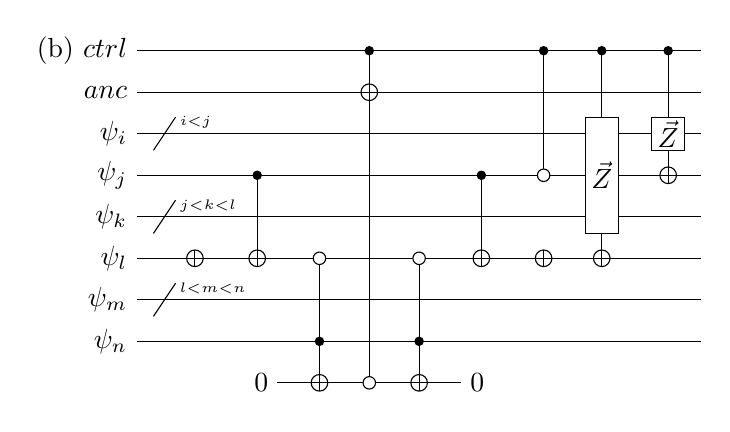
\begin{tikzpicture}[scale=1.000000,x=1pt,y=1pt]
\filldraw[color=white] (0.000000, -7.500000) rectangle (204.000000, 127.500000);
% Drawing wires
% Line 1: c W \text{(b) }ctrl
\draw[color=black] (0.000000,120.000000) -- (204.000000,120.000000);
\draw[color=black] (0.000000,120.000000) node[left] {$\text{(b) }ctrl$};
% Line 2: a W anc
\draw[color=black] (0.000000,105.000000) -- (204.000000,105.000000);
\draw[color=black] (0.000000,105.000000) node[left] {$anc$};
% Line 3: i W \psi_i
\draw[color=black] (0.000000,90.000000) -- (204.000000,90.000000);
\draw[color=black] (0.000000,90.000000) node[left] {$\psi_i$};
% Line 4: j W \psi_j
\draw[color=black] (0.000000,75.000000) -- (204.000000,75.000000);
\draw[color=black] (0.000000,75.000000) node[left] {$\psi_j$};
% Line 5: k W \psi_k
\draw[color=black] (0.000000,60.000000) -- (204.000000,60.000000);
\draw[color=black] (0.000000,60.000000) node[left] {$\psi_k$};
% Line 6: l W \psi_l
\draw[color=black] (0.000000,45.000000) -- (204.000000,45.000000);
\draw[color=black] (0.000000,45.000000) node[left] {$\psi_l$};
% Line 7: m W \psi_m
\draw[color=black] (0.000000,30.000000) -- (204.000000,30.000000);
\draw[color=black] (0.000000,30.000000) node[left] {$\psi_m$};
% Line 8: n W \psi_n
\draw[color=black] (0.000000,15.000000) -- (204.000000,15.000000);
\draw[color=black] (0.000000,15.000000) node[left] {$\psi_n$};
% Line 9: clean W 0 0
\draw[color=black] (43.500000,0.000000) -- (124.500000,0.000000);
% Done with wires; drawing gates
% Line 11: i / ^{i<j}
\draw (6.000000, 84.000000) -- (14.000000, 96.000000);
\draw (12.000000, 93.000000) node[right] {$\scriptstyle{^{i<j}}$};
% Line 12: k / ^{j<k<l}
\draw (6.000000, 54.000000) -- (14.000000, 66.000000);
\draw (12.000000, 63.000000) node[right] {$\scriptstyle{^{j<k<l}}$};
% Line 13: m / ^{l<m<n}
\draw (6.000000, 24.000000) -- (14.000000, 36.000000);
\draw (12.000000, 33.000000) node[right] {$\scriptstyle{^{l<m<n}}$};
% Line 14: c a i j k l m n clean LABEL width=-20
% Line 16: +l
\begin{scope}
\draw[fill=white] (21.000000, 45.000000) circle(3.000000pt);
\clip (21.000000, 45.000000) circle(3.000000pt);
\draw (18.000000, 45.000000) -- (24.000000, 45.000000);
\draw (21.000000, 42.000000) -- (21.000000, 48.000000);
\end{scope}
% Line 17: j +l
\draw (43.500000,75.000000) -- (43.500000,45.000000);
\filldraw (43.500000, 75.000000) circle(1.500000pt);
\begin{scope}
\draw[fill=white] (43.500000, 45.000000) circle(3.000000pt);
\clip (43.500000, 45.000000) circle(3.000000pt);
\draw (40.500000, 45.000000) -- (46.500000, 45.000000);
\draw (43.500000, 42.000000) -- (43.500000, 48.000000);
\end{scope}
% Line 18: clean START
\draw[color=black] (51.000000,0.000000) node[fill=white,left,minimum height=15.000000pt,minimum width=15.000000pt,inner sep=0pt] {\phantom{$0$}};
\draw[color=black] (51.000000,0.000000) node[left] {$0$};
% Line 19: n -l +clean
\draw (66.000000,45.000000) -- (66.000000,0.000000);
\filldraw (66.000000, 15.000000) circle(1.500000pt);
\draw[fill=white] (66.000000, 45.000000) circle(2.250000pt);
\begin{scope}
\draw[fill=white] (66.000000, 0.000000) circle(3.000000pt);
\clip (66.000000, 0.000000) circle(3.000000pt);
\draw (63.000000, 0.000000) -- (69.000000, 0.000000);
\draw (66.000000, -3.000000) -- (66.000000, 3.000000);
\end{scope}
% Line 20: c -clean +a
\draw (84.000000,120.000000) -- (84.000000,0.000000);
\filldraw (84.000000, 120.000000) circle(1.500000pt);
\draw[fill=white] (84.000000, 0.000000) circle(2.250000pt);
\begin{scope}
\draw[fill=white] (84.000000, 105.000000) circle(3.000000pt);
\clip (84.000000, 105.000000) circle(3.000000pt);
\draw (81.000000, 105.000000) -- (87.000000, 105.000000);
\draw (84.000000, 102.000000) -- (84.000000, 108.000000);
\end{scope}
% Line 21: n -l +clean
\draw (102.000000,45.000000) -- (102.000000,0.000000);
\filldraw (102.000000, 15.000000) circle(1.500000pt);
\draw[fill=white] (102.000000, 45.000000) circle(2.250000pt);
\begin{scope}
\draw[fill=white] (102.000000, 0.000000) circle(3.000000pt);
\clip (102.000000, 0.000000) circle(3.000000pt);
\draw (99.000000, 0.000000) -- (105.000000, 0.000000);
\draw (102.000000, -3.000000) -- (102.000000, 3.000000);
\end{scope}
% Line 22: clean END
\draw[color=black] (117.000000,0.000000) node[fill=white,right,minimum height=15.000000pt,minimum width=15.000000pt,inner sep=0pt] {\phantom{$0$}};
\draw[color=black] (117.000000,0.000000) node[right] {$0$};
% Line 23: j +l
\draw (124.500000,75.000000) -- (124.500000,45.000000);
\filldraw (124.500000, 75.000000) circle(1.500000pt);
\begin{scope}
\draw[fill=white] (124.500000, 45.000000) circle(3.000000pt);
\clip (124.500000, 45.000000) circle(3.000000pt);
\draw (121.500000, 45.000000) -- (127.500000, 45.000000);
\draw (124.500000, 42.000000) -- (124.500000, 48.000000);
\end{scope}
% Line 24: +l
\begin{scope}
\draw[fill=white] (147.000000, 45.000000) circle(3.000000pt);
\clip (147.000000, 45.000000) circle(3.000000pt);
\draw (144.000000, 45.000000) -- (150.000000, 45.000000);
\draw (147.000000, 42.000000) -- (147.000000, 48.000000);
\end{scope}
% Line 26: c -j
\draw (147.000000,120.000000) -- (147.000000,75.000000);
\filldraw (147.000000, 120.000000) circle(1.500000pt);
\draw[fill=white] (147.000000, 75.000000) circle(2.250000pt);
% Line 28: i j k G $\vec{Z}$ c +l
\draw (168.000000,120.000000) -- (168.000000,45.000000);
\begin{scope}
\draw[fill=white] (168.000000, 75.000000) +(-45.000000:8.485281pt and 29.698485pt) -- +(45.000000:8.485281pt and 29.698485pt) -- +(135.000000:8.485281pt and 29.698485pt) -- +(225.000000:8.485281pt and 29.698485pt) -- cycle;
\clip (168.000000, 75.000000) +(-45.000000:8.485281pt and 29.698485pt) -- +(45.000000:8.485281pt and 29.698485pt) -- +(135.000000:8.485281pt and 29.698485pt) -- +(225.000000:8.485281pt and 29.698485pt) -- cycle;
\draw (168.000000, 75.000000) node {$\vec{Z}$};
\end{scope}
\filldraw (168.000000, 120.000000) circle(1.500000pt);
\begin{scope}
\draw[fill=white] (168.000000, 45.000000) circle(3.000000pt);
\clip (168.000000, 45.000000) circle(3.000000pt);
\draw (165.000000, 45.000000) -- (171.000000, 45.000000);
\draw (168.000000, 42.000000) -- (168.000000, 48.000000);
\end{scope}
% Line 29: i G $\vec{Z}$ c +j
\draw (192.000000,120.000000) -- (192.000000,75.000000);
\begin{scope}
\draw[fill=white] (192.000000, 90.000000) +(-45.000000:8.485281pt and 8.485281pt) -- +(45.000000:8.485281pt and 8.485281pt) -- +(135.000000:8.485281pt and 8.485281pt) -- +(225.000000:8.485281pt and 8.485281pt) -- cycle;
\clip (192.000000, 90.000000) +(-45.000000:8.485281pt and 8.485281pt) -- +(45.000000:8.485281pt and 8.485281pt) -- +(135.000000:8.485281pt and 8.485281pt) -- +(225.000000:8.485281pt and 8.485281pt) -- cycle;
\draw (192.000000, 90.000000) node {$\vec{Z}$};
\end{scope}
\filldraw (192.000000, 120.000000) circle(1.500000pt);
\begin{scope}
\draw[fill=white] (192.000000, 75.000000) circle(3.000000pt);
\clip (192.000000, 75.000000) circle(3.000000pt);
\draw (189.000000, 75.000000) -- (195.000000, 75.000000);
\draw (192.000000, 72.000000) -- (192.000000, 78.000000);
\end{scope}
% Done with gates; drawing ending labels
% Done with ending labels; drawing cut lines and comments
% Done with comments
\end{tikzpicture}

    \caption{
        \textbf{Block-Encoding Product of Fermionic Operators Plus Hermitian Conjugate (modifications)}
        In subfigure a, a block-encoding for the operator $b_j b_l^\dagger + b_l b_j^\dagger$ is given.
        In subfigure b, a block-encoding for the operator $b_j b_l^\dagger b_n^\dagger b_n + b_n^\dagger b_n b_l b_j^\dagger$ is given.
    }
    \label{fig:fermionic-be-lc-modifications}
\end{figure}

For an operator with the form $b_i b_j^\dagger + b_j b_i^\dagger$, we can construct a block-encoding using with a slight modification.
In this case, we compute the variable $\ket{a}$ with the CNOT acting on the $j^\text{th}$ mode being $0$-controlled.
The circuit diagram for block-encoding this operator is given in subfigure \ref{fig:fermionic-be-lc-modifications}a.
Likewise, if a number operator is included in a term, then this can be accounted for by including a $1$-control on that mode when determining if the block-encoding ancilla should be flipped.
An example circuit diagram for an operator including a number operator is given in subfigure \ref{fig:fermionic-be-lc-modifications}b.

\begin{figure}
    \definecolor{tblue}{RGB}{61,142,221}
\definecolor{torange}{RGB}{253,143,41}
\begin{tikzpicture}[scale=1.000000,x=1pt,y=1pt]
\filldraw[color=white] (0.000000, -7.500000) rectangle (297.000000, 97.500000);
% Drawing wires
% Line 4: ctrl W ctrl
\draw[color=black] (0.000000,90.000000) -- (297.000000,90.000000);
\draw[color=black] (0.000000,90.000000) node[left] {$ctrl$};
% Line 5: anc W anc
\draw[color=black] (0.000000,75.000000) -- (297.000000,75.000000);
\draw[color=black] (0.000000,75.000000) node[left] {$anc$};
% Line 6: i W n_i
\draw[color=black] (0.000000,60.000000) -- (297.000000,60.000000);
\draw[color=black] (0.000000,60.000000) node[left] {$n_i$};
% Line 7: j W n_j
\draw[color=black] (0.000000,45.000000) -- (297.000000,45.000000);
\draw[color=black] (0.000000,45.000000) node[left] {$n_j$};
% Line 8: sys W \vdots
\draw[color=black] (0.000000,30.000000) -- (297.000000,30.000000);
\draw[color=black] (0.000000,30.000000) node[left] {$\vdots$};
% Line 9: m W n_m
\draw[color=black] (0.000000,15.000000) -- (297.000000,15.000000);
\draw[color=black] (0.000000,15.000000) node[left] {$n_m$};
% Line 10: clean W 0 0
\draw[color=black] (49.500000,0.000000) -- (130.500000,0.000000);
% Done with wires; drawing gates
% Line 12: sys +m
\draw (9.000000,30.000000) -- (9.000000,15.000000);
\filldraw (9.000000, 30.000000) circle(1.500000pt);
\begin{scope}
\draw[fill=white] (9.000000, 15.000000) circle(3.000000pt);
\clip (9.000000, 15.000000) circle(3.000000pt);
\draw (6.000000, 15.000000) -- (12.000000, 15.000000);
\draw (9.000000, 12.000000) -- (9.000000, 18.000000);
\end{scope}
% Line 13: j +sys
\draw (27.000000,45.000000) -- (27.000000,30.000000);
\filldraw (27.000000, 45.000000) circle(1.500000pt);
\begin{scope}
\draw[fill=white] (27.000000, 30.000000) circle(3.000000pt);
\clip (27.000000, 30.000000) circle(3.000000pt);
\draw (24.000000, 30.000000) -- (30.000000, 30.000000);
\draw (27.000000, 27.000000) -- (27.000000, 33.000000);
\end{scope}
% Line 14: i +j
\draw (49.500000,60.000000) -- (49.500000,45.000000);
\filldraw (49.500000, 60.000000) circle(1.500000pt);
\begin{scope}
\draw[fill=white] (49.500000, 45.000000) circle(3.000000pt);
\clip (49.500000, 45.000000) circle(3.000000pt);
\draw (46.500000, 45.000000) -- (52.500000, 45.000000);
\draw (49.500000, 42.000000) -- (49.500000, 48.000000);
\end{scope}
% Line 16: clean START
\draw[color=black] (57.000000,0.000000) node[fill=white,left,minimum height=15.000000pt,minimum width=15.000000pt,inner sep=0pt] {\phantom{$0$}};
\draw[color=black] (57.000000,0.000000) node[left] {$0$};
% Line 17: -j -sys -m +clean
\draw (72.000000,45.000000) -- (72.000000,0.000000);
\draw[fill=white] (72.000000, 45.000000) circle(2.250000pt);
\draw[fill=white] (72.000000, 30.000000) circle(2.250000pt);
\draw[fill=white] (72.000000, 15.000000) circle(2.250000pt);
\begin{scope}
\draw[fill=white] (72.000000, 0.000000) circle(3.000000pt);
\clip (72.000000, 0.000000) circle(3.000000pt);
\draw (69.000000, 0.000000) -- (75.000000, 0.000000);
\draw (72.000000, -3.000000) -- (72.000000, 3.000000);
\end{scope}
% Line 18: ctrl -clean +anc
\draw (90.000000,90.000000) -- (90.000000,0.000000);
\filldraw (90.000000, 90.000000) circle(1.500000pt);
\draw[fill=white] (90.000000, 0.000000) circle(2.250000pt);
\begin{scope}
\draw[fill=white] (90.000000, 75.000000) circle(3.000000pt);
\clip (90.000000, 75.000000) circle(3.000000pt);
\draw (87.000000, 75.000000) -- (93.000000, 75.000000);
\draw (90.000000, 72.000000) -- (90.000000, 78.000000);
\end{scope}
% Line 19: -j -sys -m +clean
\draw (108.000000,45.000000) -- (108.000000,0.000000);
\draw[fill=white] (108.000000, 45.000000) circle(2.250000pt);
\draw[fill=white] (108.000000, 30.000000) circle(2.250000pt);
\draw[fill=white] (108.000000, 15.000000) circle(2.250000pt);
\begin{scope}
\draw[fill=white] (108.000000, 0.000000) circle(3.000000pt);
\clip (108.000000, 0.000000) circle(3.000000pt);
\draw (105.000000, 0.000000) -- (111.000000, 0.000000);
\draw (108.000000, -3.000000) -- (108.000000, 3.000000);
\end{scope}
% Line 20: clean END
\draw[color=black] (123.000000,0.000000) node[fill=white,right,minimum height=15.000000pt,minimum width=15.000000pt,inner sep=0pt] {\phantom{$0$}};
\draw[color=black] (123.000000,0.000000) node[right] {$0$};
% Line 22: i +j
\draw (130.500000,60.000000) -- (130.500000,45.000000);
\filldraw (130.500000, 60.000000) circle(1.500000pt);
\begin{scope}
\draw[fill=white] (130.500000, 45.000000) circle(3.000000pt);
\clip (130.500000, 45.000000) circle(3.000000pt);
\draw (127.500000, 45.000000) -- (133.500000, 45.000000);
\draw (130.500000, 42.000000) -- (130.500000, 48.000000);
\end{scope}
% Line 23: j +sys
\draw (153.000000,45.000000) -- (153.000000,30.000000);
\filldraw (153.000000, 45.000000) circle(1.500000pt);
\begin{scope}
\draw[fill=white] (153.000000, 30.000000) circle(3.000000pt);
\clip (153.000000, 30.000000) circle(3.000000pt);
\draw (150.000000, 30.000000) -- (156.000000, 30.000000);
\draw (153.000000, 27.000000) -- (153.000000, 33.000000);
\end{scope}
% Line 27: ctrl -i color=torange
\begin{scope}[color=torange]
\draw (153.000000,90.000000) -- (153.000000,60.000000);
\filldraw (153.000000, 90.000000) circle(1.500000pt);
\draw[fill=white] (153.000000, 60.000000) circle(2.250000pt);
\end{scope}
% Line 24: sys +m
\draw (171.000000,30.000000) -- (171.000000,15.000000);
\filldraw (171.000000, 30.000000) circle(1.500000pt);
\begin{scope}
\draw[fill=white] (171.000000, 15.000000) circle(3.000000pt);
\clip (171.000000, 15.000000) circle(3.000000pt);
\draw (168.000000, 15.000000) -- (174.000000, 15.000000);
\draw (171.000000, 12.000000) -- (171.000000, 18.000000);
\end{scope}
% Line 29: i j sys G $\vec{Z}$ ctrl +m
\draw (192.000000,90.000000) -- (192.000000,15.000000);
\begin{scope}
\draw[fill=white] (192.000000, 45.000000) +(-45.000000:8.485281pt and 29.698485pt) -- +(45.000000:8.485281pt and 29.698485pt) -- +(135.000000:8.485281pt and 29.698485pt) -- +(225.000000:8.485281pt and 29.698485pt) -- cycle;
\clip (192.000000, 45.000000) +(-45.000000:8.485281pt and 29.698485pt) -- +(45.000000:8.485281pt and 29.698485pt) -- +(135.000000:8.485281pt and 29.698485pt) -- +(225.000000:8.485281pt and 29.698485pt) -- cycle;
\draw (192.000000, 45.000000) node {$\vec{Z}$};
\end{scope}
\filldraw (192.000000, 90.000000) circle(1.500000pt);
\begin{scope}
\draw[fill=white] (192.000000, 15.000000) circle(3.000000pt);
\clip (192.000000, 15.000000) circle(3.000000pt);
\draw (189.000000, 15.000000) -- (195.000000, 15.000000);
\draw (192.000000, 12.000000) -- (192.000000, 18.000000);
\end{scope}
% Line 30: ctrl i j sys LABEL ...
\draw[color=black] (217.500000, 90.000000) node [fill=white] {$\cdots$};
\draw[color=black] (217.500000, 60.000000) node [fill=white] {$\cdots$};
\draw[color=black] (217.500000, 45.000000) node [fill=white] {$\cdots$};
\draw[color=black] (217.500000, 30.000000) node [fill=white] {$\cdots$};
% Line 31: i j G $\vec{Z}$ ctrl +sys
\draw (243.000000,90.000000) -- (243.000000,30.000000);
\begin{scope}
\draw[fill=white] (243.000000, 52.500000) +(-45.000000:8.485281pt and 19.091883pt) -- +(45.000000:8.485281pt and 19.091883pt) -- +(135.000000:8.485281pt and 19.091883pt) -- +(225.000000:8.485281pt and 19.091883pt) -- cycle;
\clip (243.000000, 52.500000) +(-45.000000:8.485281pt and 19.091883pt) -- +(45.000000:8.485281pt and 19.091883pt) -- +(135.000000:8.485281pt and 19.091883pt) -- +(225.000000:8.485281pt and 19.091883pt) -- cycle;
\draw (243.000000, 52.500000) node {$\vec{Z}$};
\end{scope}
\filldraw (243.000000, 90.000000) circle(1.500000pt);
\begin{scope}
\draw[fill=white] (243.000000, 30.000000) circle(3.000000pt);
\clip (243.000000, 30.000000) circle(3.000000pt);
\draw (240.000000, 30.000000) -- (246.000000, 30.000000);
\draw (243.000000, 27.000000) -- (243.000000, 33.000000);
\end{scope}
% Line 32: i G $\vec{Z}$ ctrl +j
\draw (267.000000,90.000000) -- (267.000000,45.000000);
\begin{scope}
\draw[fill=white] (267.000000, 60.000000) +(-45.000000:8.485281pt and 8.485281pt) -- +(45.000000:8.485281pt and 8.485281pt) -- +(135.000000:8.485281pt and 8.485281pt) -- +(225.000000:8.485281pt and 8.485281pt) -- cycle;
\clip (267.000000, 60.000000) +(-45.000000:8.485281pt and 8.485281pt) -- +(45.000000:8.485281pt and 8.485281pt) -- +(135.000000:8.485281pt and 8.485281pt) -- +(225.000000:8.485281pt and 8.485281pt) -- cycle;
\draw (267.000000, 60.000000) node {$\vec{Z}$};
\end{scope}
\filldraw (267.000000, 90.000000) circle(1.500000pt);
\begin{scope}
\draw[fill=white] (267.000000, 45.000000) circle(3.000000pt);
\clip (267.000000, 45.000000) circle(3.000000pt);
\draw (264.000000, 45.000000) -- (270.000000, 45.000000);
\draw (267.000000, 42.000000) -- (267.000000, 48.000000);
\end{scope}
% Line 33: ctrl +i
\draw (288.000000,90.000000) -- (288.000000,60.000000);
\filldraw (288.000000, 90.000000) circle(1.500000pt);
\begin{scope}
\draw[fill=white] (288.000000, 60.000000) circle(3.000000pt);
\clip (288.000000, 60.000000) circle(3.000000pt);
\draw (285.000000, 60.000000) -- (291.000000, 60.000000);
\draw (288.000000, 57.000000) -- (288.000000, 63.000000);
\end{scope}
% Done with gates; drawing ending labels
% Done with ending labels; drawing cut lines and comments
% Done with comments
\end{tikzpicture}

    \caption{
        \textbf{Generalized Block-Encoding for Product of Fermionic Operators Plus Hermitian Conjugate}
        A block-encoding for the operator $b_i b_j ... b_m + b_m^\dagger ... b_j^\dagger b_i^\dagger$ is given.
        The $CZ$ gate highlighted in orange is present if $C \text{ choose } 2$ is odd where $C$ is the number of active modes excluding modes with number operators acting on them.
        Block-encodings for similar operators such as those that include number operators or different arrangements of the creation and annihilation operators can be accounted for using the modifications shown in Figure \ref{fig:fermionic-be-lc-modifications}.
    }
    \label{fig:fermionic-be-lc}
\end{figure}

The construction of these block-encoding circuits can be generalized to any operator that is a product of fermionic operators plus its hermitian conjugate.
An example circuit diagram for this generalized construction is shown in Figure \ref{fig:fermionic-be-lc}.
The $CZ$ gate that applies the sign flip on the second term that can occur when the order of the fermionic operators is swapped is only present if the number of swaps is odd.
If $C$ represents the number of active modes excluding modes where a number operator is acting on the mode, then the number of required swaps is $C \text{ choose } 2$.
In general, these block-encoding circuits will all have optimal rescaling factors ($\lambda=1$), require one block-encoding ancilla, and use $B-1$ Toffoli gates where $B$ is the number of active modes in the operator.

\begin{figure}
    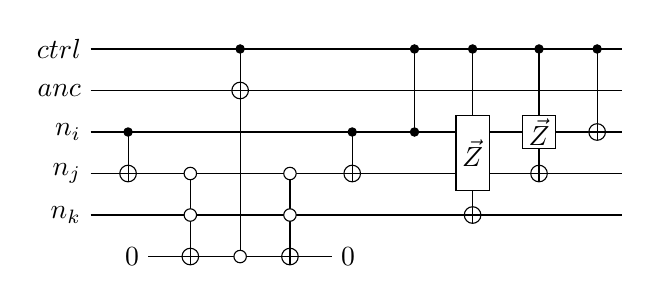
\begin{tikzpicture}[scale=1.000000,x=1pt,y=1pt]
\filldraw[color=white] (0.000000, -7.500000) rectangle (192.000000, 82.500000);
% Drawing wires
% Line 1: ctrl W ctrl
\draw[color=black] (0.000000,75.000000) -- (192.000000,75.000000);
\draw[color=black] (0.000000,75.000000) node[left] {$ctrl$};
% Line 2: anc W anc
\draw[color=black] (0.000000,60.000000) -- (192.000000,60.000000);
\draw[color=black] (0.000000,60.000000) node[left] {$anc$};
% Line 3: i W n_i
\draw[color=black] (0.000000,45.000000) -- (192.000000,45.000000);
\draw[color=black] (0.000000,45.000000) node[left] {$n_i$};
% Line 4: j W n_j
\draw[color=black] (0.000000,30.000000) -- (192.000000,30.000000);
\draw[color=black] (0.000000,30.000000) node[left] {$n_j$};
% Line 5: k W n_k
\draw[color=black] (0.000000,15.000000) -- (192.000000,15.000000);
\draw[color=black] (0.000000,15.000000) node[left] {$n_k$};
% Line 6: c1 W 0 0
\draw[color=black] (13.500000,0.000000) -- (94.500000,0.000000);
% Done with wires; drawing gates
% Line 9: i +j
\draw (13.500000,45.000000) -- (13.500000,30.000000);
\filldraw (13.500000, 45.000000) circle(1.500000pt);
\begin{scope}
\draw[fill=white] (13.500000, 30.000000) circle(3.000000pt);
\clip (13.500000, 30.000000) circle(3.000000pt);
\draw (10.500000, 30.000000) -- (16.500000, 30.000000);
\draw (13.500000, 27.000000) -- (13.500000, 33.000000);
\end{scope}
% Line 10: c1 START
\draw[color=black] (21.000000,0.000000) node[fill=white,left,minimum height=15.000000pt,minimum width=15.000000pt,inner sep=0pt] {\phantom{$0$}};
\draw[color=black] (21.000000,0.000000) node[left] {$0$};
% Line 11: -k -j +c1
\draw (36.000000,30.000000) -- (36.000000,0.000000);
\draw[fill=white] (36.000000, 15.000000) circle(2.250000pt);
\draw[fill=white] (36.000000, 30.000000) circle(2.250000pt);
\begin{scope}
\draw[fill=white] (36.000000, 0.000000) circle(3.000000pt);
\clip (36.000000, 0.000000) circle(3.000000pt);
\draw (33.000000, 0.000000) -- (39.000000, 0.000000);
\draw (36.000000, -3.000000) -- (36.000000, 3.000000);
\end{scope}
% Line 12: ctrl -c1 +anc
\draw (54.000000,75.000000) -- (54.000000,0.000000);
\filldraw (54.000000, 75.000000) circle(1.500000pt);
\draw[fill=white] (54.000000, 0.000000) circle(2.250000pt);
\begin{scope}
\draw[fill=white] (54.000000, 60.000000) circle(3.000000pt);
\clip (54.000000, 60.000000) circle(3.000000pt);
\draw (51.000000, 60.000000) -- (57.000000, 60.000000);
\draw (54.000000, 57.000000) -- (54.000000, 63.000000);
\end{scope}
% Line 13: -k -j +c1
\draw (72.000000,30.000000) -- (72.000000,0.000000);
\draw[fill=white] (72.000000, 15.000000) circle(2.250000pt);
\draw[fill=white] (72.000000, 30.000000) circle(2.250000pt);
\begin{scope}
\draw[fill=white] (72.000000, 0.000000) circle(3.000000pt);
\clip (72.000000, 0.000000) circle(3.000000pt);
\draw (69.000000, 0.000000) -- (75.000000, 0.000000);
\draw (72.000000, -3.000000) -- (72.000000, 3.000000);
\end{scope}
% Line 14: c1 END
\draw[color=black] (87.000000,0.000000) node[fill=white,right,minimum height=15.000000pt,minimum width=15.000000pt,inner sep=0pt] {\phantom{$0$}};
\draw[color=black] (87.000000,0.000000) node[right] {$0$};
% Line 15: i +j
\draw (94.500000,45.000000) -- (94.500000,30.000000);
\filldraw (94.500000, 45.000000) circle(1.500000pt);
\begin{scope}
\draw[fill=white] (94.500000, 30.000000) circle(3.000000pt);
\clip (94.500000, 30.000000) circle(3.000000pt);
\draw (91.500000, 30.000000) -- (97.500000, 30.000000);
\draw (94.500000, 27.000000) -- (94.500000, 33.000000);
\end{scope}
% Line 17: ctrl i
\draw (117.000000,75.000000) -- (117.000000,45.000000);
\filldraw (117.000000, 75.000000) circle(1.500000pt);
\filldraw (117.000000, 45.000000) circle(1.500000pt);
% Line 19: i j G $\vec{Z}$ ctrl +k
\draw (138.000000,75.000000) -- (138.000000,15.000000);
\begin{scope}
\draw[fill=white] (138.000000, 37.500000) +(-45.000000:8.485281pt and 19.091883pt) -- +(45.000000:8.485281pt and 19.091883pt) -- +(135.000000:8.485281pt and 19.091883pt) -- +(225.000000:8.485281pt and 19.091883pt) -- cycle;
\clip (138.000000, 37.500000) +(-45.000000:8.485281pt and 19.091883pt) -- +(45.000000:8.485281pt and 19.091883pt) -- +(135.000000:8.485281pt and 19.091883pt) -- +(225.000000:8.485281pt and 19.091883pt) -- cycle;
\draw (138.000000, 37.500000) node {$\vec{Z}$};
\end{scope}
\filldraw (138.000000, 75.000000) circle(1.500000pt);
\begin{scope}
\draw[fill=white] (138.000000, 15.000000) circle(3.000000pt);
\clip (138.000000, 15.000000) circle(3.000000pt);
\draw (135.000000, 15.000000) -- (141.000000, 15.000000);
\draw (138.000000, 12.000000) -- (138.000000, 18.000000);
\end{scope}
% Line 20: i G $\vec{Z}$ ctrl +j
\draw (162.000000,75.000000) -- (162.000000,30.000000);
\begin{scope}
\draw[fill=white] (162.000000, 45.000000) +(-45.000000:8.485281pt and 8.485281pt) -- +(45.000000:8.485281pt and 8.485281pt) -- +(135.000000:8.485281pt and 8.485281pt) -- +(225.000000:8.485281pt and 8.485281pt) -- cycle;
\clip (162.000000, 45.000000) +(-45.000000:8.485281pt and 8.485281pt) -- +(45.000000:8.485281pt and 8.485281pt) -- +(135.000000:8.485281pt and 8.485281pt) -- +(225.000000:8.485281pt and 8.485281pt) -- cycle;
\draw (162.000000, 45.000000) node {$\vec{Z}$};
\end{scope}
\filldraw (162.000000, 75.000000) circle(1.500000pt);
\begin{scope}
\draw[fill=white] (162.000000, 30.000000) circle(3.000000pt);
\clip (162.000000, 30.000000) circle(3.000000pt);
\draw (159.000000, 30.000000) -- (165.000000, 30.000000);
\draw (162.000000, 27.000000) -- (162.000000, 33.000000);
\end{scope}
% Line 21: ctrl +i
\draw (183.000000,75.000000) -- (183.000000,45.000000);
\filldraw (183.000000, 75.000000) circle(1.500000pt);
\begin{scope}
\draw[fill=white] (183.000000, 45.000000) circle(3.000000pt);
\clip (183.000000, 45.000000) circle(3.000000pt);
\draw (180.000000, 45.000000) -- (186.000000, 45.000000);
\draw (183.000000, 42.000000) -- (183.000000, 48.000000);
\end{scope}
% Done with gates; drawing ending labels
% Done with ending labels; drawing cut lines and comments
% Done with comments
\end{tikzpicture}

    \caption{
        \textbf{Block-Encoding for Linear Combination of Non-Conjugate Fermionic Operators}
        A block-encoding for the operator $b_i b_j b_k^\dagger + b_j^\dagger b_i^\dagger b_k^\dagger$ is given.
    }
    \label{fig:fermionic-be-lc-not-conjugate}
\end{figure}


As mentioned, the strategy employed here to construct block-encodings of a linear combination of operators is not restricted to a linear combination of hermitian conjugates.
Consider the action of the operator $b_i b_j b_k^\dagger + b_j^\dagger b_i^\dagger b_k^\dagger$ on the occupation states of the fermionic modes.
Note that the second term is not the Hermitian conjugate since the ladder operator acting on the $k^\text{th}$ mode is a creation operator in both terms.
If $\ket{a} = \ket{\psi_{b_i}} \oplus \ket{\psi_{b_j}}$, then this operator will zero-out the state \textit{unless} both $\ket{a}$ and $\ket{\psi_{b_k}}$ are $\ket{0}$.
The implementation of the block-encoding for this operator is given in Figure \ref{fig:fermionic-be-lc-not-conjugate}.
This block-encoding circuit has an optimal rescaling factor ($\lambda = 1$), requires one block-encoding ancilla, and uses two Toffoli gates.

\subsection{Bosonic Ladder Operators}

Here, we aim to define a family of unitaries ($\{U_{a^\dagger_i}, U_{a_i}\}$) that generate block-encodings of the associated bosonic creation ($a_i^\dagger$) and annihilation ($a_i$) operators.
Recall the definition of the bosonic creation operator given in Equation \ref{eq:bosonic-creation}.
From this definition, it is clear that if we rescale the operator by a factor of $\lambda = \sqrt{\Omega}$, then we can define a block-encoding unitary of the form of Eq. \ref{eq:general-block-encoding}: 
\begin{equation}
    \label{eq:be-bos-creation}
    U_{a^\dagger_i} \ket{\omega_i} \ket{0}_\text{anc} = 
    \begin{cases}
        \sqrt{\frac{\omega_i + 1}{\Omega}} \ket{\omega_i + 1} \ket{0}_\text{anc} + \beta_\psi \ket{\perp} & \text{when } \omega_i < \Omega \\
        \ket{\perp} & \text{when } \omega_i = \Omega \\
    
    \end{cases}
\end{equation}
where $\omega_i$ is the occupation number of the $i^\text{th}$ bosonic mode.

\begin{figure}
    \mbox{
        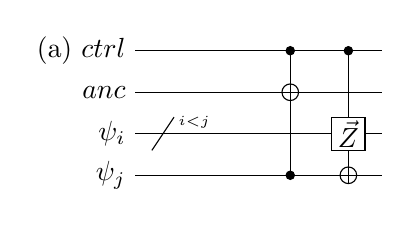
\begin{tikzpicture}[scale=1.000000,x=1pt,y=1pt]
\filldraw[color=white] (0.000000, -7.500000) rectangle (89.000000, 52.500000);
% Drawing wires
% Line 1: ctrl W \text{(a) }ctrl
\draw[color=black] (0.000000,45.000000) -- (89.000000,45.000000);
\draw[color=black] (0.000000,45.000000) node[left] {$\text{(a) }ctrl$};
% Line 2: anc W anc
\draw[color=black] (0.000000,30.000000) -- (89.000000,30.000000);
\draw[color=black] (0.000000,30.000000) node[left] {$anc$};
% Line 3: i W \psi_i
\draw[color=black] (0.000000,15.000000) -- (89.000000,15.000000);
\draw[color=black] (0.000000,15.000000) node[left] {$\psi_i$};
% Line 4: j W \psi_j
\draw[color=black] (0.000000,0.000000) -- (89.000000,0.000000);
\draw[color=black] (0.000000,0.000000) node[left] {$\psi_j$};
% Done with wires; drawing gates
% Line 6: i / ^{i<j}
\draw (6.000000, 9.000000) -- (14.000000, 21.000000);
\draw (12.000000, 18.000000) node[right] {$\scriptstyle{^{i<j}}$};
% Line 7: ctrl anc i j LABEL
% Line 8: ctrl j +anc
\draw (56.000000,45.000000) -- (56.000000,0.000000);
\filldraw (56.000000, 45.000000) circle(1.500000pt);
\filldraw (56.000000, 0.000000) circle(1.500000pt);
\begin{scope}
\draw[fill=white] (56.000000, 30.000000) circle(3.000000pt);
\clip (56.000000, 30.000000) circle(3.000000pt);
\draw (53.000000, 30.000000) -- (59.000000, 30.000000);
\draw (56.000000, 27.000000) -- (56.000000, 33.000000);
\end{scope}
% Line 10: i G $\vec{Z}$ ctrl +j
\draw (77.000000,45.000000) -- (77.000000,0.000000);
\begin{scope}
\draw[fill=white] (77.000000, 15.000000) +(-45.000000:8.485281pt and 8.485281pt) -- +(45.000000:8.485281pt and 8.485281pt) -- +(135.000000:8.485281pt and 8.485281pt) -- +(225.000000:8.485281pt and 8.485281pt) -- cycle;
\clip (77.000000, 15.000000) +(-45.000000:8.485281pt and 8.485281pt) -- +(45.000000:8.485281pt and 8.485281pt) -- +(135.000000:8.485281pt and 8.485281pt) -- +(225.000000:8.485281pt and 8.485281pt) -- cycle;
\draw (77.000000, 15.000000) node {$\vec{Z}$};
\end{scope}
\filldraw (77.000000, 45.000000) circle(1.500000pt);
\begin{scope}
\draw[fill=white] (77.000000, 0.000000) circle(3.000000pt);
\clip (77.000000, 0.000000) circle(3.000000pt);
\draw (74.000000, 0.000000) -- (80.000000, 0.000000);
\draw (77.000000, -3.000000) -- (77.000000, 3.000000);
\end{scope}
% Done with gates; drawing ending labels
% Done with ending labels; drawing cut lines and comments
% Done with comments
\end{tikzpicture}

        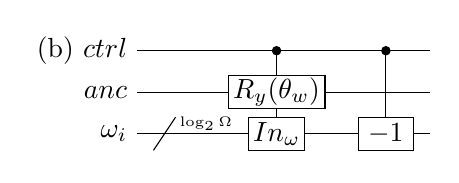
\begin{tikzpicture}[scale=1.000000,x=1pt,y=1pt]
\filldraw[color=white] (0.000000, -7.500000) rectangle (106.000000, 37.500000);
% Drawing wires
% Line 1: ctrl W \text{(b) }ctrl
\draw[color=black] (0.000000,30.000000) -- (106.000000,30.000000);
\draw[color=black] (0.000000,30.000000) node[left] {$\text{(b) }ctrl$};
% Line 2: anc W anc
\draw[color=black] (0.000000,15.000000) -- (106.000000,15.000000);
\draw[color=black] (0.000000,15.000000) node[left] {$anc$};
% Line 3: i W \omega_i
\draw[color=black] (0.000000,0.000000) -- (106.000000,0.000000);
\draw[color=black] (0.000000,0.000000) node[left] {$\omega_i$};
% Done with wires; drawing gates
% Line 5: i / ^{\log_2{\Omega}}
\draw (6.000000, -6.000000) -- (14.000000, 6.000000);
\draw (12.000000, 3.000000) node[right] {$\scriptstyle{^{\log_2{\Omega}}}$};
% Line 6: ctrl anc i LABEL width=-5
% Line 8: anc G:width=35 $R_y(\theta_w)$ i G:width=20 $In_\omega$ ctrl
\draw (50.500000,30.000000) -- (50.500000,0.000000);
\begin{scope}
\draw[fill=white] (50.500000, 15.000000) +(-45.000000:24.748737pt and 8.485281pt) -- +(45.000000:24.748737pt and 8.485281pt) -- +(135.000000:24.748737pt and 8.485281pt) -- +(225.000000:24.748737pt and 8.485281pt) -- cycle;
\clip (50.500000, 15.000000) +(-45.000000:24.748737pt and 8.485281pt) -- +(45.000000:24.748737pt and 8.485281pt) -- +(135.000000:24.748737pt and 8.485281pt) -- +(225.000000:24.748737pt and 8.485281pt) -- cycle;
\draw (50.500000, 15.000000) node {$R_y(\theta_w)$};
\end{scope}
\begin{scope}
\draw[fill=white] (50.500000, -0.000000) +(-45.000000:14.142136pt and 8.485281pt) -- +(45.000000:14.142136pt and 8.485281pt) -- +(135.000000:14.142136pt and 8.485281pt) -- +(225.000000:14.142136pt and 8.485281pt) -- cycle;
\clip (50.500000, -0.000000) +(-45.000000:14.142136pt and 8.485281pt) -- +(45.000000:14.142136pt and 8.485281pt) -- +(135.000000:14.142136pt and 8.485281pt) -- +(225.000000:14.142136pt and 8.485281pt) -- cycle;
\draw (50.500000, -0.000000) node {$In_\omega$};
\end{scope}
\filldraw (50.500000, 30.000000) circle(1.500000pt);
% Line 9: i G width=20 $-1$ ctrl
\draw (90.000000,30.000000) -- (90.000000,0.000000);
\begin{scope}
\draw[fill=white] (90.000000, -0.000000) +(-45.000000:14.142136pt and 8.485281pt) -- +(45.000000:14.142136pt and 8.485281pt) -- +(135.000000:14.142136pt and 8.485281pt) -- +(225.000000:14.142136pt and 8.485281pt) -- cycle;
\clip (90.000000, -0.000000) +(-45.000000:14.142136pt and 8.485281pt) -- +(45.000000:14.142136pt and 8.485281pt) -- +(135.000000:14.142136pt and 8.485281pt) -- +(225.000000:14.142136pt and 8.485281pt) -- cycle;
\draw (90.000000, -0.000000) node {$-1$};
\end{scope}
\filldraw (90.000000, 30.000000) circle(1.500000pt);
% Done with gates; drawing ending labels
% Done with ending labels; drawing cut lines and comments
% Done with comments
\end{tikzpicture}

    }
    \caption{
        \textbf{Bosonic Ladder Operator Block-Encoding}
        In subfigure a, a block-encoding for the bosonic creation operator, $a_i^\dagger$, is given.
        In subfigure b, a block-encoding for the bosonic annihilation operator, $a_i$, is given.
    }
    \label{fig:bosonic-ladder-op-be}
\end{figure}

The desired action of the block-encoding circuit for the bosonic creation operator is to increase the occupation of the bosonic mode by $1$ and rotate the block-encoding ancilla such that it has a coefficient of $\sqrt{\frac{\omega_i + 1}{\Omega}}$ in the $\ket{0}$ state when the occupation of the $i^\text{th}$ bosonic mode is $w_i$ prior to the operation.
This can be achieved by applying an incrementer circuit to the register encoding the occupation of the bosonic mode which increases the occupation by $1 \mod \Omega$ in each branch of the wavefunction.
The corresponding coefficients can be attained using a series of $R_y$ gates with different angles, controlled on the corresponding occupation state of the bosonic mode, and applied to the block-encoding ancilla.
An example circuit diagram for this circuit is given in subfigure \ref{fig:bosonic-ladder-op-be}a.
The angle of the $R_y$ gate can be classically determined by the following function:
\begin{equation}
    \label{eq:single-op-angles}
    \theta(\omega_i) = 
    \begin{cases} 
        2\sin^{-1}\Big(\sqrt{\frac{\omega_i}{\Omega}}\Big) & \text{when } \omega_i < \Omega\\
        0 & \text{when } \omega_i = \Omega
    \end{cases}
\end{equation}
where the choice of $\omega_i$ here in comparison with $\omega_i + 1$ in Eq. \ref{eq:be-bos-creation} is due to the occupation of the state being updated prior to these rotations.

A block-encoding circuit for the bosonic annihilation operator can be constructed similarly.
The only necessary modification is that the multiplexed rotations are applied prior to the incrementer circuit.
An example circuit diagram is given in subfigure \ref{fig:bosonic-ladder-op-be}b.

An implementation of a controlled incrementer circuit is given in \cite{Gidney_2015} which requires $\lceil \log_2\Omega \rceil$ Toffoli gates.
The series of controlled rotation gates can be implemented using a set of multiplexed rotations which can be decomposed via the protocol given in Möttönen et. al \cite{mottonen2004transformation}.
A discussion of different schemes to construct a \textit{controlled} set of multiplexed rotations is given in Appendix \ref{sec:multiplexed-rotations} and we opt for the decomposition that requires $\Omega$ uncontrolled rotations and $1$ controlled rotation.
A controlled rotation can be decomposed into $2$ uncontrolled rotations as shown in Figure \ref{fig:controlled-rotation}.
As a result, this block-encoding has a rescaling factor of $\sqrt{\Omega}$, requires one block-encoding ancilla, and uses $\lceil \log_2\Omega \rceil$ Toffoli gates and $\Omega + 2$ arbitrary rotations.


\subsection{Products of Bosonic Ladder Operators}

In this subsection, we discuss constructing block-encodings for a product of bosonic ladder operators acting on the same mode.

Unlike fermions, multiple bosons can occupy the same bosonic mode.
Therefore a bosonic ladder operator that is raised to an integer power can be applied to the state without necessarily zeroing-out the state.
Consider the desired action of a block-encoding for series of $R$ bosonic creation operators acting on the $i^\text{th}$ bosonic mode:
\begin{equation}
    \label{eq:be-S-creation-ops}
    U_{(a^\dagger_i)^R} \ket{\omega_i} \ket{0}_\text{anc} = 
    \begin{cases}
        \prod_{r=1}^{R} \sqrt{\frac{\omega_i + r}{\Omega}} \ket{\omega_i + R} \ket{0}_\text{anc} + \beta_\psi \ket{\perp} & \text{when } \omega_i \leq \Omega - R \\
        \ket{\perp} & \text{when } \omega_i > \Omega - R \\
    
    \end{cases}
\end{equation}

\begin{figure}
    \mbox{
        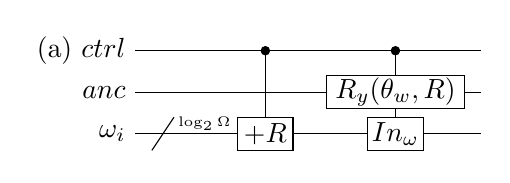
\begin{tikzpicture}[scale=1.000000,x=1pt,y=1pt]
\filldraw[color=white] (0.000000, -7.500000) rectangle (125.000000, 37.500000);
% Drawing wires
% Line 1: ctrl W \text{(a) }ctrl
\draw[color=black] (0.000000,30.000000) -- (125.000000,30.000000);
\draw[color=black] (0.000000,30.000000) node[left] {$\text{(a) }ctrl$};
% Line 2: anc W anc
\draw[color=black] (0.000000,15.000000) -- (125.000000,15.000000);
\draw[color=black] (0.000000,15.000000) node[left] {$anc$};
% Line 3: i W \omega_i
\draw[color=black] (0.000000,0.000000) -- (125.000000,0.000000);
\draw[color=black] (0.000000,0.000000) node[left] {$\omega_i$};
% Done with wires; drawing gates
% Line 5: i / ^{\log_2{\Omega}}
\draw (6.000000, -6.000000) -- (14.000000, 6.000000);
\draw (12.000000, 3.000000) node[right] {$\scriptstyle{^{\log_2{\Omega}}}$};
% Line 6: ctrl anc i LABEL width=-1
% Line 8: i G width=20 $+R$ ctrl
\draw (47.000000,30.000000) -- (47.000000,0.000000);
\begin{scope}
\draw[fill=white] (47.000000, -0.000000) +(-45.000000:14.142136pt and 8.485281pt) -- +(45.000000:14.142136pt and 8.485281pt) -- +(135.000000:14.142136pt and 8.485281pt) -- +(225.000000:14.142136pt and 8.485281pt) -- cycle;
\clip (47.000000, -0.000000) +(-45.000000:14.142136pt and 8.485281pt) -- +(45.000000:14.142136pt and 8.485281pt) -- +(135.000000:14.142136pt and 8.485281pt) -- +(225.000000:14.142136pt and 8.485281pt) -- cycle;
\draw (47.000000, -0.000000) node {$+R$};
\end{scope}
\filldraw (47.000000, 30.000000) circle(1.500000pt);
% Line 9: anc G:width=50 $R_y(\theta_w, R)$ i G:width=20 $In_\omega$ ctrl
\draw (94.000000,30.000000) -- (94.000000,0.000000);
\begin{scope}
\draw[fill=white] (94.000000, 15.000000) +(-45.000000:35.355339pt and 8.485281pt) -- +(45.000000:35.355339pt and 8.485281pt) -- +(135.000000:35.355339pt and 8.485281pt) -- +(225.000000:35.355339pt and 8.485281pt) -- cycle;
\clip (94.000000, 15.000000) +(-45.000000:35.355339pt and 8.485281pt) -- +(45.000000:35.355339pt and 8.485281pt) -- +(135.000000:35.355339pt and 8.485281pt) -- +(225.000000:35.355339pt and 8.485281pt) -- cycle;
\draw (94.000000, 15.000000) node {$R_y(\theta_w, R)$};
\end{scope}
\begin{scope}
\draw[fill=white] (94.000000, -0.000000) +(-45.000000:14.142136pt and 8.485281pt) -- +(45.000000:14.142136pt and 8.485281pt) -- +(135.000000:14.142136pt and 8.485281pt) -- +(225.000000:14.142136pt and 8.485281pt) -- cycle;
\clip (94.000000, -0.000000) +(-45.000000:14.142136pt and 8.485281pt) -- +(45.000000:14.142136pt and 8.485281pt) -- +(135.000000:14.142136pt and 8.485281pt) -- +(225.000000:14.142136pt and 8.485281pt) -- cycle;
\draw (94.000000, -0.000000) node {$In_\omega$};
\end{scope}
\filldraw (94.000000, 30.000000) circle(1.500000pt);
% Done with gates; drawing ending labels
% Done with ending labels; drawing cut lines and comments
% Done with comments
\end{tikzpicture}

        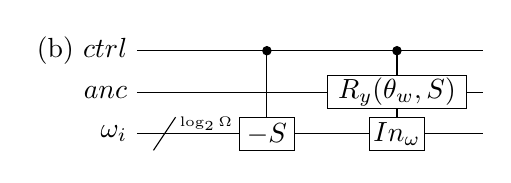
\begin{tikzpicture}[scale=1.000000,x=1pt,y=1pt]
\filldraw[color=white] (0.000000, -7.500000) rectangle (125.000000, 37.500000);
% Drawing wires
% Line 1: ctrl W \text{(b) }ctrl
\draw[color=black] (0.000000,30.000000) -- (125.000000,30.000000);
\draw[color=black] (0.000000,30.000000) node[left] {$\text{(b) }ctrl$};
% Line 2: anc W anc
\draw[color=black] (0.000000,15.000000) -- (125.000000,15.000000);
\draw[color=black] (0.000000,15.000000) node[left] {$anc$};
% Line 3: i W \omega_i
\draw[color=black] (0.000000,0.000000) -- (125.000000,0.000000);
\draw[color=black] (0.000000,0.000000) node[left] {$\omega_i$};
% Done with wires; drawing gates
% Line 5: i / ^{\log_2{\Omega}}
\draw (6.000000, -6.000000) -- (14.000000, 6.000000);
\draw (12.000000, 3.000000) node[right] {$\scriptstyle{^{\log_2{\Omega}}}$};
% Line 6: ctrl anc i LABEL width=-1
% Line 8: i G width=20 $-S$ ctrl
\draw (47.000000,30.000000) -- (47.000000,0.000000);
\begin{scope}
\draw[fill=white] (47.000000, -0.000000) +(-45.000000:14.142136pt and 8.485281pt) -- +(45.000000:14.142136pt and 8.485281pt) -- +(135.000000:14.142136pt and 8.485281pt) -- +(225.000000:14.142136pt and 8.485281pt) -- cycle;
\clip (47.000000, -0.000000) +(-45.000000:14.142136pt and 8.485281pt) -- +(45.000000:14.142136pt and 8.485281pt) -- +(135.000000:14.142136pt and 8.485281pt) -- +(225.000000:14.142136pt and 8.485281pt) -- cycle;
\draw (47.000000, -0.000000) node {$-S$};
\end{scope}
\filldraw (47.000000, 30.000000) circle(1.500000pt);
% Line 9: anc G:width=50 $R_y(\theta_w, S)$ i G:width=20 $In_\omega$ ctrl
\draw (94.000000,30.000000) -- (94.000000,0.000000);
\begin{scope}
\draw[fill=white] (94.000000, 15.000000) +(-45.000000:35.355339pt and 8.485281pt) -- +(45.000000:35.355339pt and 8.485281pt) -- +(135.000000:35.355339pt and 8.485281pt) -- +(225.000000:35.355339pt and 8.485281pt) -- cycle;
\clip (94.000000, 15.000000) +(-45.000000:35.355339pt and 8.485281pt) -- +(45.000000:35.355339pt and 8.485281pt) -- +(135.000000:35.355339pt and 8.485281pt) -- +(225.000000:35.355339pt and 8.485281pt) -- cycle;
\draw (94.000000, 15.000000) node {$R_y(\theta_w, S)$};
\end{scope}
\begin{scope}
\draw[fill=white] (94.000000, -0.000000) +(-45.000000:14.142136pt and 8.485281pt) -- +(45.000000:14.142136pt and 8.485281pt) -- +(135.000000:14.142136pt and 8.485281pt) -- +(225.000000:14.142136pt and 8.485281pt) -- cycle;
\clip (94.000000, -0.000000) +(-45.000000:14.142136pt and 8.485281pt) -- +(45.000000:14.142136pt and 8.485281pt) -- +(135.000000:14.142136pt and 8.485281pt) -- +(225.000000:14.142136pt and 8.485281pt) -- cycle;
\draw (94.000000, -0.000000) node {$In_\omega$};
\end{scope}
\filldraw (94.000000, 30.000000) circle(1.500000pt);
% Done with gates; drawing ending labels
% Done with ending labels; drawing cut lines and comments
% Done with comments
\end{tikzpicture}

    }
    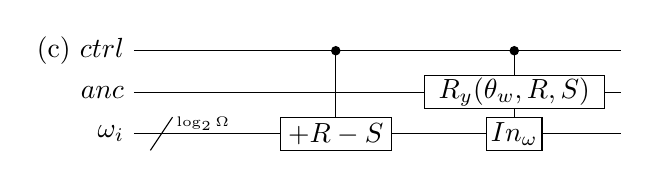
\begin{tikzpicture}[scale=1.000000,x=1pt,y=1pt]
\filldraw[color=white] (0.000000, -7.500000) rectangle (176.000000, 37.500000);
% Drawing wires
% Line 1: ctrl W \text{(c) }ctrl
\draw[color=black] (0.000000,30.000000) -- (176.000000,30.000000);
\draw[color=black] (0.000000,30.000000) node[left] {$\text{(c) }ctrl$};
% Line 2: anc W anc
\draw[color=black] (0.000000,15.000000) -- (176.000000,15.000000);
\draw[color=black] (0.000000,15.000000) node[left] {$anc$};
% Line 3: i W \omega_i
\draw[color=black] (0.000000,0.000000) -- (176.000000,0.000000);
\draw[color=black] (0.000000,0.000000) node[left] {$\omega_i$};
% Done with wires; drawing gates
% Line 5: i / ^{\log_2{\Omega}}
\draw (6.000000, -6.000000) -- (14.000000, 6.000000);
\draw (12.000000, 3.000000) node[right] {$\scriptstyle{^{\log_2{\Omega}}}$};
% Line 6: ctrl anc i LABEL
% Line 8: i G width=40 $+R-S$ ctrl
\draw (73.000000,30.000000) -- (73.000000,0.000000);
\begin{scope}
\draw[fill=white] (73.000000, -0.000000) +(-45.000000:28.284271pt and 8.485281pt) -- +(45.000000:28.284271pt and 8.485281pt) -- +(135.000000:28.284271pt and 8.485281pt) -- +(225.000000:28.284271pt and 8.485281pt) -- cycle;
\clip (73.000000, -0.000000) +(-45.000000:28.284271pt and 8.485281pt) -- +(45.000000:28.284271pt and 8.485281pt) -- +(135.000000:28.284271pt and 8.485281pt) -- +(225.000000:28.284271pt and 8.485281pt) -- cycle;
\draw (73.000000, -0.000000) node {$+R-S$};
\end{scope}
\filldraw (73.000000, 30.000000) circle(1.500000pt);
% Line 9: anc G:width=65 $R_y(\theta_w, R, S)$ i G:width=20 $In_\omega$ ctrl
\draw (137.500000,30.000000) -- (137.500000,0.000000);
\begin{scope}
\draw[fill=white] (137.500000, 15.000000) +(-45.000000:45.961941pt and 8.485281pt) -- +(45.000000:45.961941pt and 8.485281pt) -- +(135.000000:45.961941pt and 8.485281pt) -- +(225.000000:45.961941pt and 8.485281pt) -- cycle;
\clip (137.500000, 15.000000) +(-45.000000:45.961941pt and 8.485281pt) -- +(45.000000:45.961941pt and 8.485281pt) -- +(135.000000:45.961941pt and 8.485281pt) -- +(225.000000:45.961941pt and 8.485281pt) -- cycle;
\draw (137.500000, 15.000000) node {$R_y(\theta_w, R, S)$};
\end{scope}
\begin{scope}
\draw[fill=white] (137.500000, -0.000000) +(-45.000000:14.142136pt and 8.485281pt) -- +(45.000000:14.142136pt and 8.485281pt) -- +(135.000000:14.142136pt and 8.485281pt) -- +(225.000000:14.142136pt and 8.485281pt) -- cycle;
\clip (137.500000, -0.000000) +(-45.000000:14.142136pt and 8.485281pt) -- +(45.000000:14.142136pt and 8.485281pt) -- +(135.000000:14.142136pt and 8.485281pt) -- +(225.000000:14.142136pt and 8.485281pt) -- cycle;
\draw (137.500000, -0.000000) node {$In_\omega$};
\end{scope}
\filldraw (137.500000, 30.000000) circle(1.500000pt);
% Done with gates; drawing ending labels
% Done with ending labels; drawing cut lines and comments
% Done with comments
\end{tikzpicture}

    \caption{
        \textbf{Block-Encoding Product of Bosonic Ladder Operators}
        In subfigure a, a block-encoding for the operator $(a_i^\dagger)^R$ is given.
        In subfigure b, a block-encoding for the operator $(a_i)^S$ is given.
        In subfigure c, a block-encoding for the operator $(a_i^\dagger)^R (a_i)^S$ is given.
    }
    \label{fig:products-bosonic-operators}
\end{figure}

A block-encoding of this form could be achieved by simply repeating the construction for the individual bosonic creation operator (subfigure \ref{fig:bosonic-ladder-op-be}a) $R$ times.
However, a more efficient compilation can be achieved by updating the occupation of the bosonic mode by $+R$ and then performing a single series of controlled multiplexed rotations.
An example circuit diagram for this block-encoding is shown in subfigure \ref{fig:products-bosonic-operators}a.
The angles of the multiplexed rotations can be determined classically using the following function:
\begin{equation}
    \theta(\omega_i, R) = 
    \begin{cases} 
        2\sin^{-1}\Big(\prod_{r=0}^{R-1}\sqrt{\frac{\omega_i - r}{\Omega}}\Big) & \text{when } \omega_i \leq \Omega - R \\
        0 & \text{when } \omega_i > \Omega - R
    \end{cases}
\end{equation}
where the choice of $\omega_i - r$ here in comparison with $\omega_i + r$ in Eq. \ref{eq:be-S-creation-ops} is due to the occupation of the state being updated prior to these rotations.

A block-encoding for a bosonic annihilation operator being applied $S$ times can be achieved using a similar construction shown in subfigue \ref{fig:products-bosonic-operators}b.
The occupation of the mode is first decreased by $S$ and then the controlled multiplexed rotations are applied to pick up the corresponding coefficient on the block-encoding ancilla.
The function to determine the rotation angles is given by:
\begin{equation}
    \theta(\omega_i, S) = 
    \begin{cases} 
        2\sin^{-1}\Big(\prod_{s=1}^{S}\sqrt{\frac{\omega_i + s}{\Omega}}\Big) & \text{when } \omega_i \geq S \\
        0 & \text{when } \omega_i < S
    \end{cases}
\end{equation}

Likewise, we can construct a block-encoding for an operator of the form $(a_i^\dagger)^R (a_i)^S$ using a similar construction shown in subfigue \ref{fig:products-bosonic-operators}c.
The occupation of the mode is updated by a value of $+ R - S$ and then the controlled multiplexed rotations are applied to pick up the corresponding coefficient on the block-encoding ancilla.
The function to determine the rotation angles is given by:
\begin{equation}
    \theta(\omega_i, R, S) = 
    \begin{cases} 
        2\sin^{-1}\Big(\prod_{r=0}^{R-1}\sqrt{\frac{\omega_i - r}{\Omega}} \prod_{s=1}^{S}\sqrt{\frac{\omega_i - R + s}{\Omega}}\Big) & \text{when } S \leq \omega_i \leq \Omega - R \\
        0 & \text{Otherwise} 
    \end{cases}
\end{equation}

Incrementing a quantum register by a classical value can be implemented in multiple ways with different compilations having different space-time tradeoffs.
In this work, we often choose decompositions that reduce the number of non-Clifford operations at the expense or requiring more temporary ancillae, therefore we opt for the compilation given in Figure \ref{fig:addition-gate-efficient}.
This circuit requires, at most, $\lceil \log_2 \Omega \rceil - 1$ pairs of left and right elbows.
These block-encoding circuits have a rescaling factor of $\lambda = \Omega^{R+S/2}$, require one block-encoding ancilla, and use \textit{at most} $\Omega + \lceil \log_2 \Omega \rceil$ pairs of elbows and $\Omega + 2$ arbitrary rotations.


\subsection{Linear Combinations of Bosonic Ladder Operators}

In this subsection, we discuss constructing block-encodings for a linear combination of a product of bosonic ladder operators acting on the same mode plus its hermitian conjugate.

For a simple example, consider the operator $a_i^\dagger + a_i$.
Trivially, one could construct an LCO block-encoding by performing a linear combination of the block-encodings of the creation and annihilation operators respectively.
This block-encoding would have a rescaling factor of $\lambda = 2\sqrt{\Omega}$, use two block-encoding ancilla, and require $2\big(\lceil \log_2 \Omega \rceil - 1\big)$ pairs of elbows and $2 \big(\Omega + 2\big)$ arbitrary rotations.


\begin{figure}
    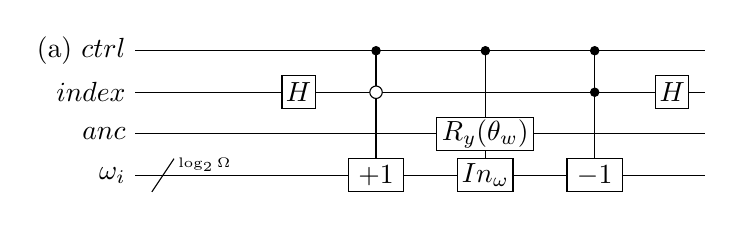
\begin{tikzpicture}[scale=1.000000,x=1pt,y=1pt]
\filldraw[color=white] (0.000000, -7.500000) rectangle (206.000000, 52.500000);
% Drawing wires
% Line 1: ctrl W \text{(a) }ctrl
\draw[color=black] (0.000000,45.000000) -- (206.000000,45.000000);
\draw[color=black] (0.000000,45.000000) node[left] {$\text{(a) }ctrl$};
% Line 2: index W index
\draw[color=black] (0.000000,30.000000) -- (206.000000,30.000000);
\draw[color=black] (0.000000,30.000000) node[left] {$index$};
% Line 3: anc W anc
\draw[color=black] (0.000000,15.000000) -- (206.000000,15.000000);
\draw[color=black] (0.000000,15.000000) node[left] {$anc$};
% Line 4: i W \omega_i
\draw[color=black] (0.000000,0.000000) -- (206.000000,0.000000);
\draw[color=black] (0.000000,0.000000) node[left] {$\omega_i$};
% Done with wires; drawing gates
% Line 6: i / ^{\log_2{\Omega}}
\draw (6.000000, -6.000000) -- (14.000000, 6.000000);
\draw (12.000000, 3.000000) node[right] {$\scriptstyle{^{\log_2{\Omega}}}$};
% Line 7: ctrl anc index i LABEL
% Line 9: index G $H$
\begin{scope}
\draw[fill=white] (59.000000, 30.000000) +(-45.000000:8.485281pt and 8.485281pt) -- +(45.000000:8.485281pt and 8.485281pt) -- +(135.000000:8.485281pt and 8.485281pt) -- +(225.000000:8.485281pt and 8.485281pt) -- cycle;
\clip (59.000000, 30.000000) +(-45.000000:8.485281pt and 8.485281pt) -- +(45.000000:8.485281pt and 8.485281pt) -- +(135.000000:8.485281pt and 8.485281pt) -- +(225.000000:8.485281pt and 8.485281pt) -- cycle;
\draw (59.000000, 30.000000) node {$H$};
\end{scope}
% Line 10: i G width=20 $+1$ ctrl -index
\draw (87.000000,45.000000) -- (87.000000,0.000000);
\begin{scope}
\draw[fill=white] (87.000000, -0.000000) +(-45.000000:14.142136pt and 8.485281pt) -- +(45.000000:14.142136pt and 8.485281pt) -- +(135.000000:14.142136pt and 8.485281pt) -- +(225.000000:14.142136pt and 8.485281pt) -- cycle;
\clip (87.000000, -0.000000) +(-45.000000:14.142136pt and 8.485281pt) -- +(45.000000:14.142136pt and 8.485281pt) -- +(135.000000:14.142136pt and 8.485281pt) -- +(225.000000:14.142136pt and 8.485281pt) -- cycle;
\draw (87.000000, -0.000000) node {$+1$};
\end{scope}
\filldraw (87.000000, 45.000000) circle(1.500000pt);
\draw[fill=white] (87.000000, 30.000000) circle(2.250000pt);
% Line 11: anc G:width=35 $R_y(\theta_w)$ i G:width=20 $In_\omega$ ctrl
\draw (126.500000,45.000000) -- (126.500000,0.000000);
\begin{scope}
\draw[fill=white] (126.500000, 15.000000) +(-45.000000:24.748737pt and 8.485281pt) -- +(45.000000:24.748737pt and 8.485281pt) -- +(135.000000:24.748737pt and 8.485281pt) -- +(225.000000:24.748737pt and 8.485281pt) -- cycle;
\clip (126.500000, 15.000000) +(-45.000000:24.748737pt and 8.485281pt) -- +(45.000000:24.748737pt and 8.485281pt) -- +(135.000000:24.748737pt and 8.485281pt) -- +(225.000000:24.748737pt and 8.485281pt) -- cycle;
\draw (126.500000, 15.000000) node {$R_y(\theta_w)$};
\end{scope}
\begin{scope}
\draw[fill=white] (126.500000, -0.000000) +(-45.000000:14.142136pt and 8.485281pt) -- +(45.000000:14.142136pt and 8.485281pt) -- +(135.000000:14.142136pt and 8.485281pt) -- +(225.000000:14.142136pt and 8.485281pt) -- cycle;
\clip (126.500000, -0.000000) +(-45.000000:14.142136pt and 8.485281pt) -- +(45.000000:14.142136pt and 8.485281pt) -- +(135.000000:14.142136pt and 8.485281pt) -- +(225.000000:14.142136pt and 8.485281pt) -- cycle;
\draw (126.500000, -0.000000) node {$In_\omega$};
\end{scope}
\filldraw (126.500000, 45.000000) circle(1.500000pt);
% Line 12: i G width=20 $-1$ ctrl index
\draw (166.000000,45.000000) -- (166.000000,0.000000);
\begin{scope}
\draw[fill=white] (166.000000, -0.000000) +(-45.000000:14.142136pt and 8.485281pt) -- +(45.000000:14.142136pt and 8.485281pt) -- +(135.000000:14.142136pt and 8.485281pt) -- +(225.000000:14.142136pt and 8.485281pt) -- cycle;
\clip (166.000000, -0.000000) +(-45.000000:14.142136pt and 8.485281pt) -- +(45.000000:14.142136pt and 8.485281pt) -- +(135.000000:14.142136pt and 8.485281pt) -- +(225.000000:14.142136pt and 8.485281pt) -- cycle;
\draw (166.000000, -0.000000) node {$-1$};
\end{scope}
\filldraw (166.000000, 45.000000) circle(1.500000pt);
\filldraw (166.000000, 30.000000) circle(1.500000pt);
% Line 13: index G $H$
\begin{scope}
\draw[fill=white] (194.000000, 30.000000) +(-45.000000:8.485281pt and 8.485281pt) -- +(45.000000:8.485281pt and 8.485281pt) -- +(135.000000:8.485281pt and 8.485281pt) -- +(225.000000:8.485281pt and 8.485281pt) -- cycle;
\clip (194.000000, 30.000000) +(-45.000000:8.485281pt and 8.485281pt) -- +(45.000000:8.485281pt and 8.485281pt) -- +(135.000000:8.485281pt and 8.485281pt) -- +(225.000000:8.485281pt and 8.485281pt) -- cycle;
\draw (194.000000, 30.000000) node {$H$};
\end{scope}
% Done with gates; drawing ending labels
% Done with ending labels; drawing cut lines and comments
% Done with comments
\end{tikzpicture}

    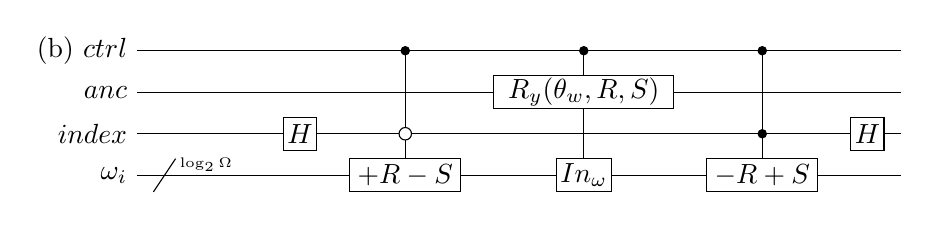
\begin{tikzpicture}[scale=1.000000,x=1pt,y=1pt]
\filldraw[color=white] (0.000000, -7.500000) rectangle (276.000000, 52.500000);
% Drawing wires
% Line 1: ctrl W \text{(b) }ctrl
\draw[color=black] (0.000000,45.000000) -- (276.000000,45.000000);
\draw[color=black] (0.000000,45.000000) node[left] {$\text{(b) }ctrl$};
% Line 2: anc W anc
\draw[color=black] (0.000000,30.000000) -- (276.000000,30.000000);
\draw[color=black] (0.000000,30.000000) node[left] {$anc$};
% Line 3: index W index
\draw[color=black] (0.000000,15.000000) -- (276.000000,15.000000);
\draw[color=black] (0.000000,15.000000) node[left] {$index$};
% Line 4: i W \omega_i
\draw[color=black] (0.000000,0.000000) -- (276.000000,0.000000);
\draw[color=black] (0.000000,0.000000) node[left] {$\omega_i$};
% Done with wires; drawing gates
% Line 6: i / ^{\log_2{\Omega}}
\draw (6.000000, -6.000000) -- (14.000000, 6.000000);
\draw (12.000000, 3.000000) node[right] {$\scriptstyle{^{\log_2{\Omega}}}$};
% Line 7: ctrl anc index i LABEL
% Line 9: index G $H$
\begin{scope}
\draw[fill=white] (59.000000, 15.000000) +(-45.000000:8.485281pt and 8.485281pt) -- +(45.000000:8.485281pt and 8.485281pt) -- +(135.000000:8.485281pt and 8.485281pt) -- +(225.000000:8.485281pt and 8.485281pt) -- cycle;
\clip (59.000000, 15.000000) +(-45.000000:8.485281pt and 8.485281pt) -- +(45.000000:8.485281pt and 8.485281pt) -- +(135.000000:8.485281pt and 8.485281pt) -- +(225.000000:8.485281pt and 8.485281pt) -- cycle;
\draw (59.000000, 15.000000) node {$H$};
\end{scope}
% Line 10: i G width=40 $+R-S$ ctrl -index
\draw (97.000000,45.000000) -- (97.000000,0.000000);
\begin{scope}
\draw[fill=white] (97.000000, -0.000000) +(-45.000000:28.284271pt and 8.485281pt) -- +(45.000000:28.284271pt and 8.485281pt) -- +(135.000000:28.284271pt and 8.485281pt) -- +(225.000000:28.284271pt and 8.485281pt) -- cycle;
\clip (97.000000, -0.000000) +(-45.000000:28.284271pt and 8.485281pt) -- +(45.000000:28.284271pt and 8.485281pt) -- +(135.000000:28.284271pt and 8.485281pt) -- +(225.000000:28.284271pt and 8.485281pt) -- cycle;
\draw (97.000000, -0.000000) node {$+R-S$};
\end{scope}
\filldraw (97.000000, 45.000000) circle(1.500000pt);
\draw[fill=white] (97.000000, 15.000000) circle(2.250000pt);
% Line 11: anc G:width=65 $R_y(\theta_w, R, S)$ i G:width=20 $In_\omega$ ctrl
\draw (161.500000,45.000000) -- (161.500000,0.000000);
\begin{scope}
\draw[fill=white] (161.500000, 30.000000) +(-45.000000:45.961941pt and 8.485281pt) -- +(45.000000:45.961941pt and 8.485281pt) -- +(135.000000:45.961941pt and 8.485281pt) -- +(225.000000:45.961941pt and 8.485281pt) -- cycle;
\clip (161.500000, 30.000000) +(-45.000000:45.961941pt and 8.485281pt) -- +(45.000000:45.961941pt and 8.485281pt) -- +(135.000000:45.961941pt and 8.485281pt) -- +(225.000000:45.961941pt and 8.485281pt) -- cycle;
\draw (161.500000, 30.000000) node {$R_y(\theta_w, R, S)$};
\end{scope}
\begin{scope}
\draw[fill=white] (161.500000, -0.000000) +(-45.000000:14.142136pt and 8.485281pt) -- +(45.000000:14.142136pt and 8.485281pt) -- +(135.000000:14.142136pt and 8.485281pt) -- +(225.000000:14.142136pt and 8.485281pt) -- cycle;
\clip (161.500000, -0.000000) +(-45.000000:14.142136pt and 8.485281pt) -- +(45.000000:14.142136pt and 8.485281pt) -- +(135.000000:14.142136pt and 8.485281pt) -- +(225.000000:14.142136pt and 8.485281pt) -- cycle;
\draw (161.500000, -0.000000) node {$In_\omega$};
\end{scope}
\filldraw (161.500000, 45.000000) circle(1.500000pt);
% Line 12: i G width=40 $-R+S$ ctrl index
\draw (226.000000,45.000000) -- (226.000000,0.000000);
\begin{scope}
\draw[fill=white] (226.000000, -0.000000) +(-45.000000:28.284271pt and 8.485281pt) -- +(45.000000:28.284271pt and 8.485281pt) -- +(135.000000:28.284271pt and 8.485281pt) -- +(225.000000:28.284271pt and 8.485281pt) -- cycle;
\clip (226.000000, -0.000000) +(-45.000000:28.284271pt and 8.485281pt) -- +(45.000000:28.284271pt and 8.485281pt) -- +(135.000000:28.284271pt and 8.485281pt) -- +(225.000000:28.284271pt and 8.485281pt) -- cycle;
\draw (226.000000, -0.000000) node {$-R+S$};
\end{scope}
\filldraw (226.000000, 45.000000) circle(1.500000pt);
\filldraw (226.000000, 15.000000) circle(1.500000pt);
% Line 13: index G $H$
\begin{scope}
\draw[fill=white] (264.000000, 15.000000) +(-45.000000:8.485281pt and 8.485281pt) -- +(45.000000:8.485281pt and 8.485281pt) -- +(135.000000:8.485281pt and 8.485281pt) -- +(225.000000:8.485281pt and 8.485281pt) -- cycle;
\clip (264.000000, 15.000000) +(-45.000000:8.485281pt and 8.485281pt) -- +(45.000000:8.485281pt and 8.485281pt) -- +(135.000000:8.485281pt and 8.485281pt) -- +(225.000000:8.485281pt and 8.485281pt) -- cycle;
\draw (264.000000, 15.000000) node {$H$};
\end{scope}
% Done with gates; drawing ending labels
% Done with ending labels; drawing cut lines and comments
% Done with comments
\end{tikzpicture}

    \caption{
        \textbf{Block-Encoding Product of Bosonic Ladder Operators Plus Hermitian Conjugate}
        In subfigure a, a block-encoding for the operator $(a_i^\dagger + a_i)$ is given.
        In subfigure b, a block-encoding for the operator $\big((a_i^\dagger)^R (a_i)^S + (a_i^\dagger)^S (a_i)^R\big)$ is given.
    }
    \label{fig:lc-bosonic}
\end{figure}


Due to the symmetry of the block-encodings for the individual operators, we can produce a more gate-efficient compilation.
For the annihilation operator, we wish to decrease the occupancy by $1$ and then apply the rotations.
Whereas for the creation operator, we wish in apply the rotations and then increase the occupancy by $1$.
Since the desired rotation angles are independent of which operator is being applied (Eq. \ref{eq:single-op-angles}), we can reuse the multiplexed rotations to apply the appropriate angles for both terms.
An example circuit diagram for this block-encoding is shown in subfigue \ref{fig:lc-bosonic}a.
Similarly, a block-encoding for the generalized operator $\big((a_i^\dagger)^R (a_i)^S + (a_i^\dagger)^S (a_i)^R\big)$ can be constructed and is shown in subfigure \ref{fig:lc-bosonic}b.

This compilation strategy is chosen under the assumption that the cost of implementing the multiplexed rotations exceeds the cost of the incrementer circuit.
If the inverse were true, a compilation could be constructed where the incrementer circuit is reused for both terms and the multiplexed rotations would be applied twice.  

For these block-encoding circuits, one additional pair of elbows is required to index between the two controlled incrementer circuits in Figure \ref{fig:lc-bosonic}.
Therefore, these block-encodings have a rescaling factor of $\lambda = 2 \Omega^{R+S/2}$, use two block-encoding ancilla, and require $\Omega + 2\big(\lceil \log_2 \Omega \rceil\big)$ pairs of elbows and $\Omega + 2$ arbitrary rotations.

\subsection{Terms with Fermionic and Bosonic Ladder Operators}

In the previous subsections, we discussed strategies for compiling block-encodings of different products and linear combinations of ladder operators acting on either fermionic or bosonic modes.
In this subsection, we discuss how to generate block-encodings for operators that contain both fermionic and bosonic operators.

\begin{figure}
    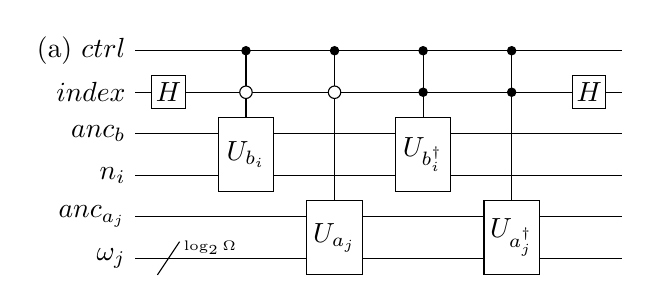
\begin{tikzpicture}[scale=1.000000,x=1pt,y=1pt]
\filldraw[color=white] (0.000000, -7.500000) rectangle (176.000000, 82.500000);
% Drawing wires
% Line 1: ctrl W \text{(a) }ctrl
\draw[color=black] (0.000000,75.000000) -- (176.000000,75.000000);
\draw[color=black] (0.000000,75.000000) node[left] {$\text{(a) }ctrl$};
% Line 2: index W index
\draw[color=black] (0.000000,60.000000) -- (176.000000,60.000000);
\draw[color=black] (0.000000,60.000000) node[left] {$index$};
% Line 3: anc_b W anc_b
\draw[color=black] (0.000000,45.000000) -- (176.000000,45.000000);
\draw[color=black] (0.000000,45.000000) node[left] {$anc_b$};
% Line 4: i W n_i
\draw[color=black] (0.000000,30.000000) -- (176.000000,30.000000);
\draw[color=black] (0.000000,30.000000) node[left] {$n_i$};
% Line 5: anc_a W anc_{a_j}
\draw[color=black] (0.000000,15.000000) -- (176.000000,15.000000);
\draw[color=black] (0.000000,15.000000) node[left] {$anc_{a_j}$};
% Line 6: j W \omega_j
\draw[color=black] (0.000000,0.000000) -- (176.000000,0.000000);
\draw[color=black] (0.000000,0.000000) node[left] {$\omega_j$};
% Done with wires; drawing gates
% Line 8: j / ^{\log_2{\Omega}}
\draw (8.000000, -6.000000) -- (16.000000, 6.000000);
\draw (14.000000, 3.000000) node[right] {$\scriptstyle{^{\log_2{\Omega}}}$};
% Line 10: index G $H$
\begin{scope}
\draw[fill=white] (12.000000, 60.000000) +(-45.000000:8.485281pt and 8.485281pt) -- +(45.000000:8.485281pt and 8.485281pt) -- +(135.000000:8.485281pt and 8.485281pt) -- +(225.000000:8.485281pt and 8.485281pt) -- cycle;
\clip (12.000000, 60.000000) +(-45.000000:8.485281pt and 8.485281pt) -- +(45.000000:8.485281pt and 8.485281pt) -- +(135.000000:8.485281pt and 8.485281pt) -- +(225.000000:8.485281pt and 8.485281pt) -- cycle;
\draw (12.000000, 60.000000) node {$H$};
\end{scope}
% Line 11: i anc_b G width=20 $U_{b_i}$ ctrl -index
\draw (40.000000,75.000000) -- (40.000000,30.000000);
\begin{scope}
\draw[fill=white] (40.000000, 37.500000) +(-45.000000:14.142136pt and 19.091883pt) -- +(45.000000:14.142136pt and 19.091883pt) -- +(135.000000:14.142136pt and 19.091883pt) -- +(225.000000:14.142136pt and 19.091883pt) -- cycle;
\clip (40.000000, 37.500000) +(-45.000000:14.142136pt and 19.091883pt) -- +(45.000000:14.142136pt and 19.091883pt) -- +(135.000000:14.142136pt and 19.091883pt) -- +(225.000000:14.142136pt and 19.091883pt) -- cycle;
\draw (40.000000, 37.500000) node {$U_{b_i}$};
\end{scope}
\filldraw (40.000000, 75.000000) circle(1.500000pt);
\draw[fill=white] (40.000000, 60.000000) circle(2.250000pt);
% Line 12: j anc_a G width=20 $U_{a_j}$ ctrl -index
\draw (72.000000,75.000000) -- (72.000000,0.000000);
\begin{scope}
\draw[fill=white] (72.000000, 7.500000) +(-45.000000:14.142136pt and 19.091883pt) -- +(45.000000:14.142136pt and 19.091883pt) -- +(135.000000:14.142136pt and 19.091883pt) -- +(225.000000:14.142136pt and 19.091883pt) -- cycle;
\clip (72.000000, 7.500000) +(-45.000000:14.142136pt and 19.091883pt) -- +(45.000000:14.142136pt and 19.091883pt) -- +(135.000000:14.142136pt and 19.091883pt) -- +(225.000000:14.142136pt and 19.091883pt) -- cycle;
\draw (72.000000, 7.500000) node {$U_{a_j}$};
\end{scope}
\filldraw (72.000000, 75.000000) circle(1.500000pt);
\draw[fill=white] (72.000000, 60.000000) circle(2.250000pt);
% Line 13: i anc_b G width=20 $U_{b_i^\dagger}$ ctrl index
\draw (104.000000,75.000000) -- (104.000000,30.000000);
\begin{scope}
\draw[fill=white] (104.000000, 37.500000) +(-45.000000:14.142136pt and 19.091883pt) -- +(45.000000:14.142136pt and 19.091883pt) -- +(135.000000:14.142136pt and 19.091883pt) -- +(225.000000:14.142136pt and 19.091883pt) -- cycle;
\clip (104.000000, 37.500000) +(-45.000000:14.142136pt and 19.091883pt) -- +(45.000000:14.142136pt and 19.091883pt) -- +(135.000000:14.142136pt and 19.091883pt) -- +(225.000000:14.142136pt and 19.091883pt) -- cycle;
\draw (104.000000, 37.500000) node {$U_{b_i^\dagger}$};
\end{scope}
\filldraw (104.000000, 75.000000) circle(1.500000pt);
\filldraw (104.000000, 60.000000) circle(1.500000pt);
% Line 14: j anc_a G width=20 $U_{a_j^\dagger}$ ctrl index
\draw (136.000000,75.000000) -- (136.000000,0.000000);
\begin{scope}
\draw[fill=white] (136.000000, 7.500000) +(-45.000000:14.142136pt and 19.091883pt) -- +(45.000000:14.142136pt and 19.091883pt) -- +(135.000000:14.142136pt and 19.091883pt) -- +(225.000000:14.142136pt and 19.091883pt) -- cycle;
\clip (136.000000, 7.500000) +(-45.000000:14.142136pt and 19.091883pt) -- +(45.000000:14.142136pt and 19.091883pt) -- +(135.000000:14.142136pt and 19.091883pt) -- +(225.000000:14.142136pt and 19.091883pt) -- cycle;
\draw (136.000000, 7.500000) node {$U_{a_j^\dagger}$};
\end{scope}
\filldraw (136.000000, 75.000000) circle(1.500000pt);
\filldraw (136.000000, 60.000000) circle(1.500000pt);
% Line 15: index G $H$
\begin{scope}
\draw[fill=white] (164.000000, 60.000000) +(-45.000000:8.485281pt and 8.485281pt) -- +(45.000000:8.485281pt and 8.485281pt) -- +(135.000000:8.485281pt and 8.485281pt) -- +(225.000000:8.485281pt and 8.485281pt) -- cycle;
\clip (164.000000, 60.000000) +(-45.000000:8.485281pt and 8.485281pt) -- +(45.000000:8.485281pt and 8.485281pt) -- +(135.000000:8.485281pt and 8.485281pt) -- +(225.000000:8.485281pt and 8.485281pt) -- cycle;
\draw (164.000000, 60.000000) node {$H$};
\end{scope}
% Done with gates; drawing ending labels
% Done with ending labels; drawing cut lines and comments
% Done with comments
\end{tikzpicture}

    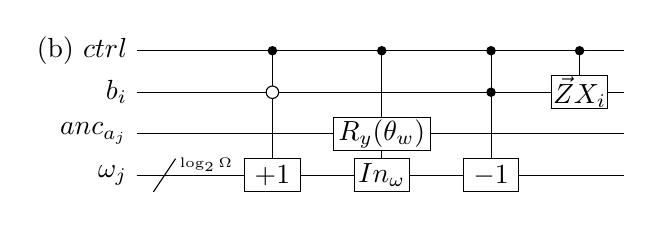
\begin{tikzpicture}[scale=1.000000,x=1pt,y=1pt]
\filldraw[color=white] (0.000000, -7.500000) rectangle (176.000000, 52.500000);
% Drawing wires
% Line 1: ctrl W \text{(b) }ctrl
\draw[color=black] (0.000000,45.000000) -- (176.000000,45.000000);
\draw[color=black] (0.000000,45.000000) node[left] {$\text{(b) }ctrl$};
% Line 2: i W b_i
\draw[color=black] (0.000000,30.000000) -- (176.000000,30.000000);
\draw[color=black] (0.000000,30.000000) node[left] {$b_i$};
% Line 3: anc_a W anc_{a_j}
\draw[color=black] (0.000000,15.000000) -- (176.000000,15.000000);
\draw[color=black] (0.000000,15.000000) node[left] {$anc_{a_j}$};
% Line 4: j W \omega_j
\draw[color=black] (0.000000,0.000000) -- (176.000000,0.000000);
\draw[color=black] (0.000000,0.000000) node[left] {$\omega_j$};
% Done with wires; drawing gates
% Line 6: j / ^{\log_2{\Omega}}
\draw (6.000000, -6.000000) -- (14.000000, 6.000000);
\draw (12.000000, 3.000000) node[right] {$\scriptstyle{^{\log_2{\Omega}}}$};
% Line 7: ctrl i anc_a j LABEL width=1
% Line 9: j G width=20 $+1$ ctrl -i
\draw (49.000000,45.000000) -- (49.000000,0.000000);
\begin{scope}
\draw[fill=white] (49.000000, -0.000000) +(-45.000000:14.142136pt and 8.485281pt) -- +(45.000000:14.142136pt and 8.485281pt) -- +(135.000000:14.142136pt and 8.485281pt) -- +(225.000000:14.142136pt and 8.485281pt) -- cycle;
\clip (49.000000, -0.000000) +(-45.000000:14.142136pt and 8.485281pt) -- +(45.000000:14.142136pt and 8.485281pt) -- +(135.000000:14.142136pt and 8.485281pt) -- +(225.000000:14.142136pt and 8.485281pt) -- cycle;
\draw (49.000000, -0.000000) node {$+1$};
\end{scope}
\filldraw (49.000000, 45.000000) circle(1.500000pt);
\draw[fill=white] (49.000000, 30.000000) circle(2.250000pt);
% Line 10: anc_a G:width=35 $R_y(\theta_w)$ j G:width=20 $In_\omega$ ctrl
\draw (88.500000,45.000000) -- (88.500000,0.000000);
\begin{scope}
\draw[fill=white] (88.500000, 15.000000) +(-45.000000:24.748737pt and 8.485281pt) -- +(45.000000:24.748737pt and 8.485281pt) -- +(135.000000:24.748737pt and 8.485281pt) -- +(225.000000:24.748737pt and 8.485281pt) -- cycle;
\clip (88.500000, 15.000000) +(-45.000000:24.748737pt and 8.485281pt) -- +(45.000000:24.748737pt and 8.485281pt) -- +(135.000000:24.748737pt and 8.485281pt) -- +(225.000000:24.748737pt and 8.485281pt) -- cycle;
\draw (88.500000, 15.000000) node {$R_y(\theta_w)$};
\end{scope}
\begin{scope}
\draw[fill=white] (88.500000, -0.000000) +(-45.000000:14.142136pt and 8.485281pt) -- +(45.000000:14.142136pt and 8.485281pt) -- +(135.000000:14.142136pt and 8.485281pt) -- +(225.000000:14.142136pt and 8.485281pt) -- cycle;
\clip (88.500000, -0.000000) +(-45.000000:14.142136pt and 8.485281pt) -- +(45.000000:14.142136pt and 8.485281pt) -- +(135.000000:14.142136pt and 8.485281pt) -- +(225.000000:14.142136pt and 8.485281pt) -- cycle;
\draw (88.500000, -0.000000) node {$In_\omega$};
\end{scope}
\filldraw (88.500000, 45.000000) circle(1.500000pt);
% Line 11: j G width=20 $-1$ ctrl i
\draw (128.000000,45.000000) -- (128.000000,0.000000);
\begin{scope}
\draw[fill=white] (128.000000, -0.000000) +(-45.000000:14.142136pt and 8.485281pt) -- +(45.000000:14.142136pt and 8.485281pt) -- +(135.000000:14.142136pt and 8.485281pt) -- +(225.000000:14.142136pt and 8.485281pt) -- cycle;
\clip (128.000000, -0.000000) +(-45.000000:14.142136pt and 8.485281pt) -- +(45.000000:14.142136pt and 8.485281pt) -- +(135.000000:14.142136pt and 8.485281pt) -- +(225.000000:14.142136pt and 8.485281pt) -- cycle;
\draw (128.000000, -0.000000) node {$-1$};
\end{scope}
\filldraw (128.000000, 45.000000) circle(1.500000pt);
\filldraw (128.000000, 30.000000) circle(1.500000pt);
% Line 13: i G width=20 $\vec{Z}X_i$ ctrl
\draw (160.000000,45.000000) -- (160.000000,30.000000);
\begin{scope}
\draw[fill=white] (160.000000, 30.000000) +(-45.000000:14.142136pt and 8.485281pt) -- +(45.000000:14.142136pt and 8.485281pt) -- +(135.000000:14.142136pt and 8.485281pt) -- +(225.000000:14.142136pt and 8.485281pt) -- cycle;
\clip (160.000000, 30.000000) +(-45.000000:14.142136pt and 8.485281pt) -- +(45.000000:14.142136pt and 8.485281pt) -- +(135.000000:14.142136pt and 8.485281pt) -- +(225.000000:14.142136pt and 8.485281pt) -- cycle;
\draw (160.000000, 30.000000) node {$\vec{Z}X_i$};
\end{scope}
\filldraw (160.000000, 45.000000) circle(1.500000pt);
% Done with gates; drawing ending labels
% Done with ending labels; drawing cut lines and comments
% Done with comments
\end{tikzpicture}

    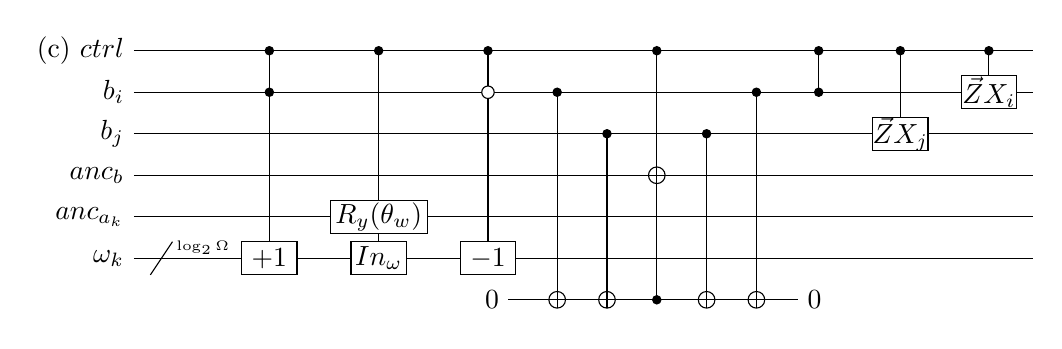
\begin{tikzpicture}[scale=1.000000,x=1pt,y=1pt]
\filldraw[color=white] (0.000000, -7.500000) rectangle (325.000000, 97.500000);
% Drawing wires
% Line 1: ctrl W \text{(c) }ctrl
\draw[color=black] (0.000000,90.000000) -- (325.000000,90.000000);
\draw[color=black] (0.000000,90.000000) node[left] {$\text{(c) }ctrl$};
% Line 2: i W b_i
\draw[color=black] (0.000000,75.000000) -- (325.000000,75.000000);
\draw[color=black] (0.000000,75.000000) node[left] {$b_i$};
% Line 3: j W b_j
\draw[color=black] (0.000000,60.000000) -- (325.000000,60.000000);
\draw[color=black] (0.000000,60.000000) node[left] {$b_j$};
% Line 4: anc_b W anc_b
\draw[color=black] (0.000000,45.000000) -- (325.000000,45.000000);
\draw[color=black] (0.000000,45.000000) node[left] {$anc_b$};
% Line 5: anc_a W anc_{a_k}
\draw[color=black] (0.000000,30.000000) -- (325.000000,30.000000);
\draw[color=black] (0.000000,30.000000) node[left] {$anc_{a_k}$};
% Line 6: k W \omega_k
\draw[color=black] (0.000000,15.000000) -- (325.000000,15.000000);
\draw[color=black] (0.000000,15.000000) node[left] {$\omega_k$};
% Line 7: c0 W 0 0
\draw[color=black] (128.000000,0.000000) -- (247.500000,0.000000);
% Done with wires; drawing gates
% Line 9: k / ^{\log_2{\Omega}}
\draw (6.000000, 9.000000) -- (14.000000, 21.000000);
\draw (12.000000, 18.000000) node[right] {$\scriptstyle{^{\log_2{\Omega}}}$};
% Line 10: ctrl i j anc_b anc_a k c0 LABEL width=1
% Line 12: k G width=20 $+1$ ctrl i
\draw (49.000000,90.000000) -- (49.000000,15.000000);
\begin{scope}
\draw[fill=white] (49.000000, 15.000000) +(-45.000000:14.142136pt and 8.485281pt) -- +(45.000000:14.142136pt and 8.485281pt) -- +(135.000000:14.142136pt and 8.485281pt) -- +(225.000000:14.142136pt and 8.485281pt) -- cycle;
\clip (49.000000, 15.000000) +(-45.000000:14.142136pt and 8.485281pt) -- +(45.000000:14.142136pt and 8.485281pt) -- +(135.000000:14.142136pt and 8.485281pt) -- +(225.000000:14.142136pt and 8.485281pt) -- cycle;
\draw (49.000000, 15.000000) node {$+1$};
\end{scope}
\filldraw (49.000000, 90.000000) circle(1.500000pt);
\filldraw (49.000000, 75.000000) circle(1.500000pt);
% Line 13: anc_a G:width=35 $R_y(\theta_w)$ k G:width=20 $In_\omega$ ctrl
\draw (88.500000,90.000000) -- (88.500000,15.000000);
\begin{scope}
\draw[fill=white] (88.500000, 30.000000) +(-45.000000:24.748737pt and 8.485281pt) -- +(45.000000:24.748737pt and 8.485281pt) -- +(135.000000:24.748737pt and 8.485281pt) -- +(225.000000:24.748737pt and 8.485281pt) -- cycle;
\clip (88.500000, 30.000000) +(-45.000000:24.748737pt and 8.485281pt) -- +(45.000000:24.748737pt and 8.485281pt) -- +(135.000000:24.748737pt and 8.485281pt) -- +(225.000000:24.748737pt and 8.485281pt) -- cycle;
\draw (88.500000, 30.000000) node {$R_y(\theta_w)$};
\end{scope}
\begin{scope}
\draw[fill=white] (88.500000, 15.000000) +(-45.000000:14.142136pt and 8.485281pt) -- +(45.000000:14.142136pt and 8.485281pt) -- +(135.000000:14.142136pt and 8.485281pt) -- +(225.000000:14.142136pt and 8.485281pt) -- cycle;
\clip (88.500000, 15.000000) +(-45.000000:14.142136pt and 8.485281pt) -- +(45.000000:14.142136pt and 8.485281pt) -- +(135.000000:14.142136pt and 8.485281pt) -- +(225.000000:14.142136pt and 8.485281pt) -- cycle;
\draw (88.500000, 15.000000) node {$In_\omega$};
\end{scope}
\filldraw (88.500000, 90.000000) circle(1.500000pt);
% Line 14: k G width=20 $-1$ ctrl -i
\draw (128.000000,90.000000) -- (128.000000,15.000000);
\begin{scope}
\draw[fill=white] (128.000000, 15.000000) +(-45.000000:14.142136pt and 8.485281pt) -- +(45.000000:14.142136pt and 8.485281pt) -- +(135.000000:14.142136pt and 8.485281pt) -- +(225.000000:14.142136pt and 8.485281pt) -- cycle;
\clip (128.000000, 15.000000) +(-45.000000:14.142136pt and 8.485281pt) -- +(45.000000:14.142136pt and 8.485281pt) -- +(135.000000:14.142136pt and 8.485281pt) -- +(225.000000:14.142136pt and 8.485281pt) -- cycle;
\draw (128.000000, 15.000000) node {$-1$};
\end{scope}
\filldraw (128.000000, 90.000000) circle(1.500000pt);
\draw[fill=white] (128.000000, 75.000000) circle(2.250000pt);
% Line 16: c0 START
\draw[color=black] (135.500000,0.000000) node[fill=white,left,minimum height=15.000000pt,minimum width=15.000000pt,inner sep=0pt] {\phantom{$0$}};
\draw[color=black] (135.500000,0.000000) node[left] {$0$};
% Line 17: i +c0
\draw (153.000000,75.000000) -- (153.000000,0.000000);
\filldraw (153.000000, 75.000000) circle(1.500000pt);
\begin{scope}
\draw[fill=white] (153.000000, 0.000000) circle(3.000000pt);
\clip (153.000000, 0.000000) circle(3.000000pt);
\draw (150.000000, 0.000000) -- (156.000000, 0.000000);
\draw (153.000000, -3.000000) -- (153.000000, 3.000000);
\end{scope}
% Line 18: j +c0
\draw (171.000000,60.000000) -- (171.000000,0.000000);
\filldraw (171.000000, 60.000000) circle(1.500000pt);
\begin{scope}
\draw[fill=white] (171.000000, 0.000000) circle(3.000000pt);
\clip (171.000000, 0.000000) circle(3.000000pt);
\draw (168.000000, 0.000000) -- (174.000000, 0.000000);
\draw (171.000000, -3.000000) -- (171.000000, 3.000000);
\end{scope}
% Line 19: ctrl c0 +anc_b
\draw (189.000000,90.000000) -- (189.000000,0.000000);
\filldraw (189.000000, 90.000000) circle(1.500000pt);
\filldraw (189.000000, 0.000000) circle(1.500000pt);
\begin{scope}
\draw[fill=white] (189.000000, 45.000000) circle(3.000000pt);
\clip (189.000000, 45.000000) circle(3.000000pt);
\draw (186.000000, 45.000000) -- (192.000000, 45.000000);
\draw (189.000000, 42.000000) -- (189.000000, 48.000000);
\end{scope}
% Line 20: j +c0
\draw (207.000000,60.000000) -- (207.000000,0.000000);
\filldraw (207.000000, 60.000000) circle(1.500000pt);
\begin{scope}
\draw[fill=white] (207.000000, 0.000000) circle(3.000000pt);
\clip (207.000000, 0.000000) circle(3.000000pt);
\draw (204.000000, 0.000000) -- (210.000000, 0.000000);
\draw (207.000000, -3.000000) -- (207.000000, 3.000000);
\end{scope}
% Line 21: i +c0
\draw (225.000000,75.000000) -- (225.000000,0.000000);
\filldraw (225.000000, 75.000000) circle(1.500000pt);
\begin{scope}
\draw[fill=white] (225.000000, 0.000000) circle(3.000000pt);
\clip (225.000000, 0.000000) circle(3.000000pt);
\draw (222.000000, 0.000000) -- (228.000000, 0.000000);
\draw (225.000000, -3.000000) -- (225.000000, 3.000000);
\end{scope}
% Line 22: c0 END
\draw[color=black] (240.000000,0.000000) node[fill=white,right,minimum height=15.000000pt,minimum width=15.000000pt,inner sep=0pt] {\phantom{$0$}};
\draw[color=black] (240.000000,0.000000) node[right] {$0$};
% Line 24: ctrl i
\draw (247.500000,90.000000) -- (247.500000,75.000000);
\filldraw (247.500000, 90.000000) circle(1.500000pt);
\filldraw (247.500000, 75.000000) circle(1.500000pt);
% Line 26: j G width=20 $\vec{Z}X_j$ ctrl
\draw (277.000000,90.000000) -- (277.000000,60.000000);
\begin{scope}
\draw[fill=white] (277.000000, 60.000000) +(-45.000000:14.142136pt and 8.485281pt) -- +(45.000000:14.142136pt and 8.485281pt) -- +(135.000000:14.142136pt and 8.485281pt) -- +(225.000000:14.142136pt and 8.485281pt) -- cycle;
\clip (277.000000, 60.000000) +(-45.000000:14.142136pt and 8.485281pt) -- +(45.000000:14.142136pt and 8.485281pt) -- +(135.000000:14.142136pt and 8.485281pt) -- +(225.000000:14.142136pt and 8.485281pt) -- cycle;
\draw (277.000000, 60.000000) node {$\vec{Z}X_j$};
\end{scope}
\filldraw (277.000000, 90.000000) circle(1.500000pt);
% Line 27: i G width=20 $\vec{Z}X_i$ ctrl
\draw (309.000000,90.000000) -- (309.000000,75.000000);
\begin{scope}
\draw[fill=white] (309.000000, 75.000000) +(-45.000000:14.142136pt and 8.485281pt) -- +(45.000000:14.142136pt and 8.485281pt) -- +(135.000000:14.142136pt and 8.485281pt) -- +(225.000000:14.142136pt and 8.485281pt) -- cycle;
\clip (309.000000, 75.000000) +(-45.000000:14.142136pt and 8.485281pt) -- +(45.000000:14.142136pt and 8.485281pt) -- +(135.000000:14.142136pt and 8.485281pt) -- +(225.000000:14.142136pt and 8.485281pt) -- cycle;
\draw (309.000000, 75.000000) node {$\vec{Z}X_i$};
\end{scope}
\filldraw (309.000000, 90.000000) circle(1.500000pt);
% Done with gates; drawing ending labels
% Done with ending labels; drawing cut lines and comments
% Done with comments
\end{tikzpicture}

    \caption{
        \textbf{Block-Encoding Terms}
        In subfigure a, a naive block-encoding for the operator $b_i a_j + a_j^\dagger b_i^\dagger$ is given.
        In subfigure b, a block-encoding for the operator $\big((a_i^\dagger)^R (a_i)^S + (a_i^\dagger)^S (a_i)^R\big)$ is given.
    }
    \label{fig:be-term-example}
\end{figure}


As an example, consider the operator: $b_i a_j + a_j^\dagger b_i^\dagger$.
Using Theorems \ref{th:product} and \ref{th:lco} to construct block-encodings of the individual terms and then combining them together would have a rescaling factor of $\lambda = 2*\sqrt{\Omega}$ and use $3$ block-encoding ancillae.
Additionally, the non-Clifford gate-cost would be $3$ Toffoli gates, 2 controlled incrementers, and $2*\Omega$ arbitrary rotations.
A circuit diagram for this construction is given in subfigure \ref{fig:be-term-example}a.

However, we can instead block-encode the entire operator at once by noting the action of the conjoined operator on the different occupation states of the fermionic mode.
Using the circuit shown in subfigure \ref{fig:be-term-example}b, the occupation of the fermionic mode is used to determine which bosonic operator is applied to the bosonic mode.
If the fermionic mode is occupied, then the bosonic annihilation operator is applied to apply the term $b_i a_j$.
If the fermionic mode is unoccupied, then the bosonic creation operator is applied to apply the term $b_i^\dagger a_j^\dagger$.
This block-encoding will have a rescaling factor of $\lambda = \sqrt{\Omega}$, use $1$ block-encoding ancillae, and require $1$ Toffoli gate, $2$ controlled incrementers, and $\Omega$ arbitrary rotations.

This strategy can be employed for other combinations of bosonic and fermionic ladder operators.
In the full Yukawa model, the operator $b_i b_j a_k^\dagger + b_j^\dagger b_i^\dagger a_k$ is used to describe the process of a fermion and antifermion being annihilated to form a boson as well as a boson being annihilated to form a fermion and antifermion.
For this operator, the occupation of either mode can be used to dictate which bosonic operator is applied to the system.
If both modes are occupied, then the bosonic creation operator should be applied.
If both modes are unoccupied, then the bosonic annihilation operator should be applied.
If the occupation of the two modes are not the same, then the state will be zeroed-out and the block-encoding ancilla for the fermionic modes will be flipped outside of the encoded subspace, therefore the action performed on the bosonic state will not matter.
A circuit diagram for this block-encoding is shown in subfigure \ref{fig:be-term-example}c.
This block-encoding has a rescaling factor of $\lambda = \sqrt{\Omega}$, uses $2$ block-encoding ancillae, and requires $2$ Toffolis, $2$ controlled incrementers, and $\Omega$ arbitrary rotations.



\section{Ladder Operator Block-Encoding}
\label{sec:lobe}

\ws{How do we block-encode a second-quantized hamiltonian?}

\ws{
    \begin{enumerate}
        \item Second-quantized Hamiltonians are LCLOs
        \item Block-encoding construction using sparse-lc hybrid
        \item Rescaling term coefficients to ensure consistent rescaling factor
        \item Explicit construction/definition of oracles (prepare for rescaled coefficieints, select/oc for rescaled terms)
        \item Comment on making select self-inverse
        \item Define overall rescaling factor
    \end{enumerate}
}


\section{Compilation and Resource Estimation}

\subsection{Prepare Oracle}

\ws{ASP/Grover-Rudolph w/Multiplexed Rotations}

\subsection{Select Oracle}

\subsubsection{Multiplexing over index register}

\subsubsection{Fermionic Ladder Oracles}

\ws{Replacing coefficient qubit + rotation with controls on the system register}

\subsubsection{Bosonic Ladder Oracles}
\ws{Bosonic coefficient rotations as controlled multiplexed rotations}
\ws{Updating occupancy using controlled addition by a classical value}

\section{Results}
\label{sec:results}

In this section, we demonstrate the use of LOBE to block-encode Hamiltonians derived from quantum field theories: Yukawa theory and $\phi^4$ theory \cite{Peskin:1995ev}.
We study both variants of the block-encoding described in Sections \ref{sec:block-encoding} and expanded upon in Section \ref{sec:lobe} and give numerical counts for the numbers of non-Clifford operations, the number of ancillae required beyond the system register, and the rescaling factor imposed on the resulting block-encoding.

The results that we present here are generated based on constructions of LOBE that are written in Cirq \cite{cirq} and the block-encodings are numerically verified for circuits of up to 14 qubits.
Additionally, the operators are constructed through the use of OpenParticle \cite{openparticle}, a software library for the construction and manipulation of fermionic, antifermionic, and bosonic ladder operators.
The software library \cite{grover-rudolph-github} is used to determine the rotation angles required for Grover-Rudolph.

\subsection{Yukawa Theory}
A quantum field theory that models the strong nuclear force between hadrons is Yukawa theory \cite{Peskin:1995ev}. In this theory, hadrons are described by a fermionic field $\psi$, coupled via a scalar boson $\phi$. The interaction term is $\mathcal{L}_{\text{Yukawa}} = g\bar\psi \psi \phi$, which leads to interaction vertices containing fermions and/or antifermions and bosons. The Lagrangian, and thus the Hamiltonian, is written as a sum of free, non-ineteracting fields and the interaction term.

Utilizing the lightfront frame \cite{Dirac1949}, leads to a straightforward approach to writing down the Hamiltonian bound-state eigenvalue equation in terms of ladder operators. This lightfront frame removes the ambiguous $\sqrt{\nabla^2 + m^2}$ term that appears in a canonical, instant-time frame Hamiltonian approach. 

The interaction terms in the Hamiltonian are $H_{\text{Yukawa int}} \in \{b^\dagger b a, b^\dagger b a^\dagger, d^\dagger d a, d^\dagger d a^\dagger, b^\dagger d^\dagger a, bda^\dagger, b^\dagger b a^\dagger a, d^\dagger d a^\dagger a \}$, while the free part of the Hamiltonian is $H_{\text{free}} \in \{b^\dagger b, d^\dagger d, a^\dagger a \}$. 
Much of the interesting physics arises from the interacting piece. The terms $b^\dagger b a$ and $b^\dagger b a^\dagger$ describe the annihilation of a fermion with a boson and creation of a fermion, and the creation of a fermion-boson pair from a fermion respectively. $d^\dagger d a$ and $d^\dagger d a^\dagger$ describe the same interactions but for antifermions and bosons. 
$b^\dagger d^\dagger a$ and $bda^\dagger$ correspond to fermion-antifermion pair creation and annihilation, and lastly, $b^\dagger b a^\dagger a$ and $d^\dagger d a^\dagger a$ are terms of $\mathcal{O}(g^2)$, unique to the lighfront frame.

This Hamiltonian can be written out as a discrete sum over these free and interaction ladder operators with coefficients coming from lightfront coordinates. The Hamiltonian can be written as:

\begin{equation}
    \label{eq:Yukawa-hamiltonian}
    H_{\text{Yukawa}} = H_0 + H_{\bar\psi \psi \phi}.
\end{equation}
The explicit form of the Hamiltonian will be written out in the appendix. 

\begin{figure}
    \centering
    \includegraphics[width=16cm]{figures/Yukawa_hamiltonian_gates_vs_terms.pdf}
    \caption{
        \textbf{Numerical Gate Counts for Increasing $L$ (Yukawa Hamiltonian).}
        The number of rotations (left), left-elbows (middle), and right-elbows (right) are plotted as a function of the number of terms in the Hamiltonian ($L$) for an increasing number of momentum modes ($I$).
        The gate counts for the variant of LOBE using \textit{USP} are shown as the blue squares.
        The gate counts for the variant of LOBE using \textit{ASP} are shown as the orange circles.
        The bosonic occupancy cutoff ($\Omega$) is set to $3$.
        The number of rotations excludes rotations by angles that result in Clifford operations.
    }
    \label{fig:Yukawa_hamiltonian_gates_vs_terms}
\end{figure}
\begin{figure}
    \centering
    \includegraphics[width=12cm]{figures/Yukawa_hamiltonian_qubits_and_rescaling_vs_terms.pdf}
    \caption{
        \textbf{Numerical Ancillae Counts and Rescaling Factors for Increasing $L$ (Yukawa Hamiltonian).}
        The number of required ancillae (left) and the resulting rescaling factor (right) for LOBE are plotted as a function of the number of terms in the Hamiltonian ($L$) for an increasing number of momentum modes ($I$).
        The counts for the variant of LOBE using \textit{USP} are shown as the blue squares.
        The counts for the variant of LOBE using \textit{ASP} are shown as the orange circles.
        The bosonic occupancy cutoff ($\Omega$) is set to $3$.
    }
    \label{fig:Yukawa_hamiltonian_qubits_and_rescaling_vs_terms}
\end{figure}

In Figure \ref{fig:Yukawa_hamiltonian_gates_vs_terms}, we plot the numerical gate counts estimates for the Yukawa Hamiltonian (Eq. \ref{eq:Yukawa-hamiltonian}) as the number of terms in the Hamiltonain ($L$) increases.
The number of terms ($L$) increases directly with an increasing number of momentum modes as $\mathcal{O}(I^3)$
For the three non-Clifford operations, the number of operations increases linearly with the number of terms in the Hamiltonian for this model.
Additionally, the two different compilation strategies (\textit{USP} (blue), \textit{ASP} (orange)) demonstrate the same numerical scaling and have nearly identical gate counts for all types of operations.
When the number of terms ($L$) is far from the next largest power of 2, \textit{ASP} requires more arbitrary rotations due to the compilation of Grover-Rudolph and multiplexed rotations that is used in this work.

In Figure \ref{fig:Yukawa_hamiltonian_qubits_and_rescaling_vs_terms}, we plot the numerical estimates for the number of required ancillae (left) and the imposed rescaling factor (right) as the number of terms in the Hamiltonain ($L$) increases.
The number of ancillae grows logarithmically with the number of terms for both implementations.
The number of ancillae used for the index register grows logarithmically with the number of terms which accounts for this scaling.
The main advantage of the \textit{ASP} variant is the effect on the rescaling factor of the block-encoding.
While the rescaling factor of both variants seemingly grows linearly with respect to the number of terms in the Hamiltonian, the rescaling factor for the \textit{ASP} variant is significantly smaller than the \textit{USP} variant.
When block-encodings are employed as a subroutine in larger algorithms, the quantum resources for the algorithm are often dependent on the rescaling factor (with a lower rescaling factor generally being preferred).
For example, in the context of using Quantum Phase Estimation to estimate the eigenvalues of a Hamiltonian, the number of gates required typically scales as $O(\frac{1}{\lambda})$ \cite{babbush2018encoding}. 
However, the exact cost associated with the rescaling factor is difficult to determine without choosing a specific algorithm to benchmark with.

\begin{figure}
    \centering
    \includegraphics[width=16cm]{figures/Yukawa_hamiltonian_gates_vs_omega.pdf}
    \caption{
        \textbf{Numerical Gate Counts for Increasing $\Omega$ (Yukawa Hamiltonian) .}
        The number of rotations (left), left-elbows (middle), and right-elbows (right) are plotted as a function of the bosonic occupation cutoff ($\Omega$).
        The gate counts for the variant of LOBE using \textit{USP} are shown as the blue squares.
        The gate counts for the variant of LOBE using \textit{ASP} are shown as the orange circles.
        The number of momentum modes ($I$) is set to $2$.
        The number of rotations excludes rotations by angles that result in Clifford operations.
    }
    \label{fig:Yukawa_hamiltonian_gates_vs_omega}
\end{figure}
\begin{figure}
    \centering
    \includegraphics[width=12cm]{figures/Yukawa_hamiltonian_qubits_and_rescaling_vs_omega.pdf}
    \caption{
        \textbf{Numerical Ancillae Counts and Rescaling Factors for Increasing $\Omega$ (Yukawa Hamiltonian).}
        The number of required ancillae (left) and the resulting rescaling factor (right) for LOBE are plotted as a function of the bosonic occupation cutoff ($\Omega$).
        The counts for the variant of LOBE using \textit{USP} are shown as the blue squares.
        The counts for the variant of LOBE using \textit{ASP} are shown as the orange circles.
        The number of momentum modes ($I$) is set to $2$.
    }
    \label{fig:Yukawa_hamiltonian_qubits_and_rescaling_vs_omega}
\end{figure}

In Figure \ref{fig:Yukawa_hamiltonian_gates_vs_omega}, we plot the numerical gate counts estimates for the Yukawa Hamiltonian (Eq. \ref{eq:Yukawa-hamiltonian}) as the cutoff on the maximum bosonic occupation ($\Omega$) increases.
For the three non-Clifford operations, the number of operations increases linearly with the bosonic occupancy cutoff for this model.
Similar to the case with increasing $I$, the two different compilation strategies (\textit{USP} (blue), \textit{ASP} orange) demonstrate the same numerical scaling and have nearly identical gate counts for all types of operations.

In Figure \ref{fig:Yukawa_hamiltonian_qubits_and_rescaling_vs_omega}, we plot the numerical estimates for the number of required ancillae (left) and the imposed rescaling factor (right) as the cutoff on the maximum bosonic occupation ($\Omega$) increases.
The number of ancillae grows logarithmically with the bosonic occupation cutoff for both implementations.
The number of ancillae needed to update the bosonic occupancy grows logarithmically with $\Omega$ (Eq. \ref{eq:ancillae-bosonic-updates}) which accounts for this scaling.
Again, the main advantage of the \textit{ASP} variant is that the imposed rescaling factor is significantly smaller than the \textit{USP} variant, especially for large values of $\Omega$ despite the asymptotic scaling being linear for both.


\subsection{$\phi^4$ Theory}
\gus{@kamil}
\subsection{Quartic Oscillator Results}
\label{sec:qosc_results}

The quartic oscillator \cite{PhysRev.184.1231, girguś2024spiralflowquantumquartic, wójcik2012applicationnumericalrenormalizationgroup} is an extension of the standard harmonic oscillator, modified by an additional non-linearity of the form $\lambda \varphi^4$, leading to the Hamiltonian $H = \frac12\dot\phi^2 + \frac{m}{2}\phi^2 + gm^3\phi^4 $, where $\phi$ represents a bosonic field composed of a single mode.
In a second-quantized, dimensionless form, the Hamiltonian can be written as:

\begin{equation}
    \label{eq:qosc}
    H = a^\dagger a + g\left(a + a^\dagger \right)^4
\end{equation}

It should be obvious that the Hamiltonian written in equation \ref{eq:qosc} is a valid form that can be block-encoded with LOBE, where there is one mode, which can be chosen implicitly to be $0$.
The only `scaling' variable in this problem is the occupancy of the mode $0$, $\Omega$.

\begin{figure}[h]
    \centering
    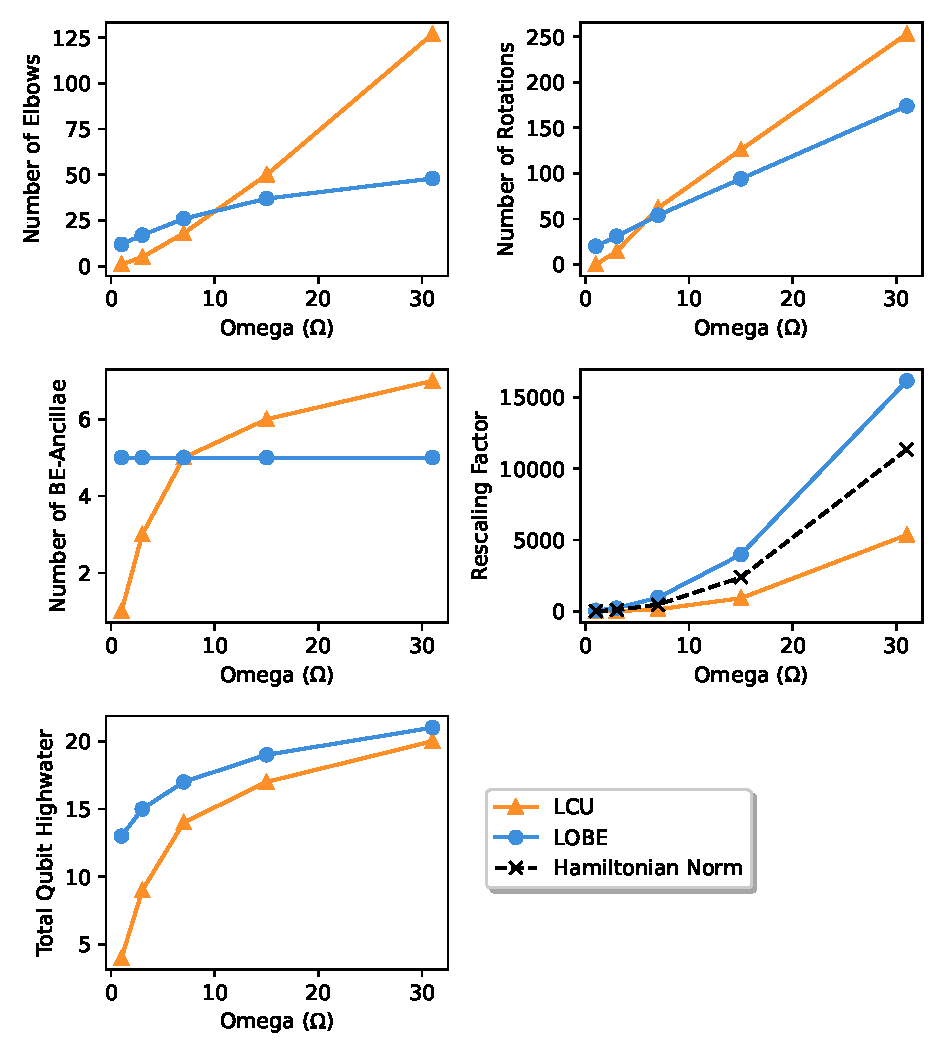
\includegraphics[width = 15cm]{figures/quartic_oscillator.pdf}
    \caption{Costs associated with a single block encoding of the quartic oscillator Hamiltonian \ref{eq:qosc} for LOBE (blue) and LCU (orange).}
    \label{fig:qosc}
\end{figure}

\subsection{Massive Static Yukawa Results}
\label{sec:static_yukawa}

Before looking at results for the simplest interacting quantum field theory composed of fermions \textit{and} bosons, the Yukawa model, we look at a non-relativistic approximation to this theory, the static yukawa model \cite{PhysRevD.103.014021}.
This model is taken as the limit of full Yukawa of infinitely heavy fermions, and bosons at rest relative to the fermions that emit/absorb them.

The second-quantized Hamiltonian for this model is 

\begin{equation}
    \label{eq:static-yukawa}
    H = C_f b^\dagger b + C_b a^\dagger a + g b^\dagger b \left( a + a^\dagger \right)
\end{equation}
 
Similar to the quartic oscillator results, both the fermion and bosons are defined on a single mode, with the only scaling variable of the model taken to be $\Omega$.

\begin{figure}[h]
    \centering
    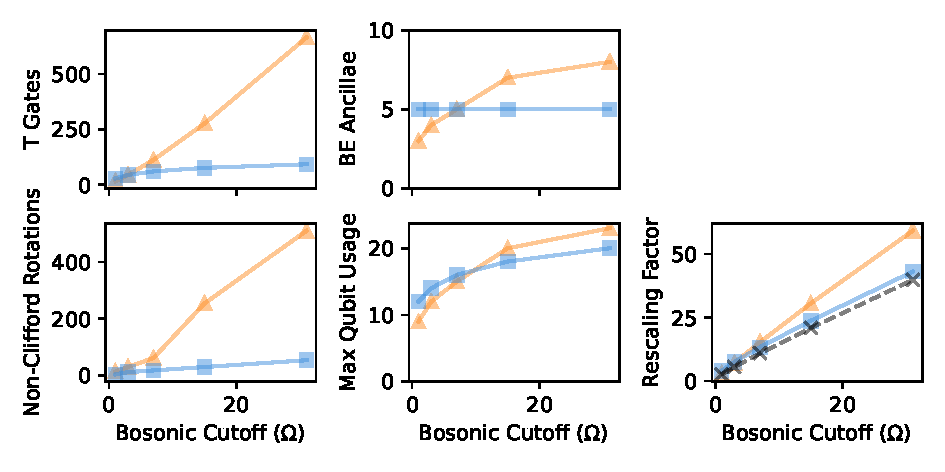
\includegraphics[width = 15cm]{figures/static_yukawa.pdf}
    \caption{Costs associated with a single block encoding of the static Yukawa Hamiltonian \ref{eq:static-yukawa} for LOBE (blue) and LCU (orange).}
    \label{fig:qosc}
\end{figure}
\subsection{$\phi^4$ Results}
\label{sec:phi4_results}

The first interesting relativistic Hamiltonian studied with LOBE is $\phi^4$ theory. 
Any field theory is defined at the level of a Lagrangian, which for $\phi^4$ theory is given as
\begin{equation}
    \mathcal{L} = \frac12 \left(\partial_\mu \phi \right)^2 - \frac{m^2}{2}\phi^2 - g\phi^4.
\end{equation}

To obtain a Hamiltonian from a Lagrangian, a Legendre transformation is performed, in which an explicit set of coordinates must be chosen. 
The set of coordinates used in this paper, which lead to the simplest forms of the corresponding Hamiltonians, are front form (lightfront) coordinates \cite{Dirac1949}.
A discussion on lightfront coordinates, as well as the corresponding Hamiltonians for each theory studied will be given in appendix \ref{subsec:lightfront-hamiltonian}.

Obscuring the coefficients, which can be found in appendix \ref{subsec:lightfront-hamiltonian}, the $\phi^4$ Hamiltonian can be written as:

\begin{align}
    H = \sum_i c_i a_i^\dagger a_i + \sum_{ijkl}c_{ijkl} \left(a_i^\dagger a_j^\dagger a_k^\dagger a_l + h.c. \right) + \sum_{ijkl}c_{ijkl}a_i^\dagger a_j^\dagger a_k a_l
\end{align}

Unlike the non-relativistic theories, both relativistic theories are defined over many modes.
Thus, the results will be given as two sets of plots: one set of cost vs. \textit{resolution} (a discussion on resolution is given in the appendix. For those uninterested, this can be loosely thought of as number of modes), and one set of cost vs occupancy ($\Omega$.)

\begin{figure}[h]
    \centering
    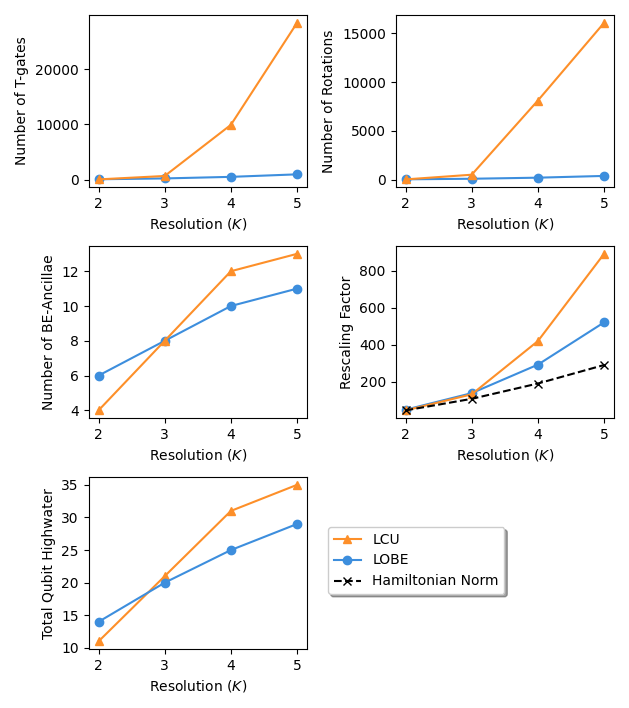
\includegraphics[width = 15cm]{figures/phi4_resolutions.png}
    \caption{}
    \label{}
\end{figure}

\begin{figure}[h]
    \centering
    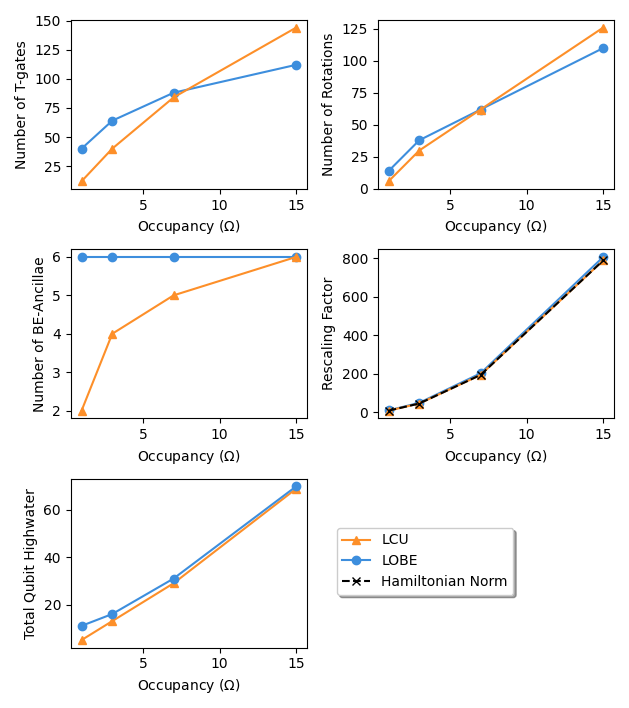
\includegraphics[width = 15cm]{figures/phi4_occupancies.png}
    \caption{}
    \label{}
\end{figure}
\subsection{Full Yukawa Results}
\label{sec:yukawa_results}

The first interacting field theory between different types of particles studied is generally the Yukawa model.
This is a theory of interacting fermions and bosons which can be used as a model of the strong nuclear force between hadrons.
The Lagrangian for this model is given as

\begin{equation}
    \label{eq:yukawa-lagrangian}
    \mathcal{L} = \bar \psi \left(i\gamma^\mu \partial_\mu - m \right)\psi + \frac{1}{2}\partial_\mu \phi \partial^\mu \phi - \frac{1}{2}\mu^2\phi^2 - g\bar \psi \psi \phi,
\end{equation}


\section{Conclusions}
\label{sec:conclusions}


\section{Acknowledgements}

Wop, wop, wop, wop, wop, Dot, fuck 'em up

Wop, wop, wop, wop, wop, I'ma do my stuff
\cite{Lamar_2024}

\bibliography{refs/citations}

\appendix

\section{Glossary}
\label{sec:glossary}

In this Section, we explicitly define some of the technical phrases and symbols used throughout this work.

\begin{itemize}
    \item \textit{term} ($T$): An operator defined as a product of ladder operators.
    \item \textit{Active Mode}: A fermionic or bosonic mode upon which a ladder operator is being non-trivially applied. 
    \item \textit{block-encoding ancillae}: A register of qubits that give additional degrees of freedom to produce a block-encoding for the operator in a larger Hilbert space.
    \item \textit{``zeroed-out"}: When the coefficient of a state becomes zero due to the application of an operator.
    \item \textit{encoded subspace}: The chosen subspace of the block-encoding ancillae that denotes the subspace in which the non-unitary operator is encoded. Typically, this is the subspace where all block-encoding ancillae are in the $\ket{0}$ state.
    \item \textit{clean ancillae}: A register of qubits that are promised to begin in the $\ket{0}$ and are returned to the $\ket{0}$ state at the end of a particular operation. 
    \item \textit{all-zero state}: A state of a register where all qubits are in the $\ket{0}$ state.
    \item $L$: The number of terms in the Hamiltonian.
    \item $\alpha_l$: The coefficient of the $l^\text{th}$ term in a linear combination. Assumed to be real and positive unless otherwise stated.
    \item $\Omega$: The occupation cutoff for the bosonic modes. $\Omega$ gives the maximum number of bosons that can be present in a single mode. 
    \item $I$: The number of fermionic or bosonic modes. The subscripts $b$ and $a$ will be used to denote the number of fermionic and bosonic modes respectively.
    \item $b_i$: Fermionic annihilation (creation - $b_i^\dagger$) operator acting on mode $i$.
    \item $d_i$: Antifermionic annihilation (creation - $d_i^\dagger$) operator acting on mode $i$.
    \item $a_i$: Bosonic annihilation (creation - $a_i^\dagger$) operator acting on mode $i$.
    \item $n_{i_b}$: The number of fermions ($b$) occupying the $i^{th}$ mode. $n_{i_d}$ and $n_{i_a}$ give the occupancy for antifermions and bosons respectively.
    \item $\omega_{i}$: The number of bosons occupying the $i^{th}$ bosonic mode.
    \item $N_A$: The dimension of a matrix $A$.
    \item $\beta_\psi$: The amplitude of a state that is outside of the encoded subspace after a block-encoding unitary is applied to $\ket{\psi}$.
    \item $\lambda$: The rescaling factor imposed on the operator for a given block-encoding.
    \item $w$: The index of the $w^\text{th}$ least-significant bit in a binary encoding.
    \item $B$: The number of active modes within a term. The  with ladder operators acting on them within the term $T_l$.
    \item $C$: The number of active modes within a term \textit{excluding} modes upon which a number operator is being applied.
    \item $S_{l, i}$: The exponent of bosonic annihilation operators acting on the $i^{th}$ bosonic mode within the $l^{th}$ term.
    \item $R_{l, i}$: The exponent of bosonic creation operators acting on the $i^{th}$ bosonic mode within the $l^{th}$ term.
    \item $P$: The sum of the exponents of bosonic ladder operators acting on all modes within a single term.
\end{itemize}
\section{Proof of $\lambda_{ASP} \leq \lambda_{USP}$}
\label{sec:proof-of-rescaling-factors}

\begin{theorem}
    $\lambda_{ASP} \leq \lambda_{USP}$
\end{theorem}

\textbf{Proof:} 

Define the following:
\begin{equation}
    \lambda_{USP} \equiv L\max_l|\tilde{\alpha}_l|
\end{equation}
and
\begin{equation}
    \lambda_{ASP} = \sum_l |\tilde{\alpha}_l|
\end{equation}

\textit{Case 1: All Coefficients are Equal}

Assume $\tilde{\alpha}_i = \tilde{\alpha}_j \forall i,j$.
Let $\tilde{\alpha}_i = \tilde{\alpha}$.
Then, $\lambda_{USP} \equiv L\max_l|\tilde{\alpha}_l| = L|\tilde{\alpha}|$ and $\sum_{l = 0}^{L - 1}|\tilde{\alpha}_l| = L|\tilde{\alpha}|$.
Thus, in this case, $\lambda_{USP} = \lambda_{ASP}$.

\textit{Case 2: Coefficients are Not All Equal}

Assume that there exist at least two coefficients, $\tilde{\alpha}_i$ and $\tilde{\alpha}_j$ such that $\tilde{\alpha}_i \neq \tilde{\alpha}_j$.
This implies that at least one coefficient, $\alpha_l$, has the largest magnitude.
Then, $\lambda_{ASP} = max_l|\tilde{\alpha}_l| + \sum_{k \neq l}|\tilde{\alpha}_k|$.
Now, if $\lambda_{ASP} < \lambda_{USP}$, then $\lambda_{ASP} - \lambda_{USP} < 0$:
\begin{align}
    \lambda_{ASP} - \lambda_{USP} &= max_l|\tilde{\alpha}_l| + \sum_{k \neq l}|\tilde{\alpha}_k| - Lmax_l|\tilde{\alpha}_l|\\ \nonumber
                                &= -(L - 1)max_l|\tilde{\alpha}_l|+ \sum_{k \neq l}|\tilde{\alpha}_k| \\ \nonumber
                                &< -(L - 1)max_l|\tilde{\alpha}_l| + \sum_{k \neq l}max_l|\tilde{\alpha}_l| \\ \nonumber
                                &= -(L - 1)max_l|\tilde{\alpha}_l| + (L - 1) max_l|\tilde{\alpha}_l|\\ \nonumber
                                &= 0 \\ \nonumber
\end{align}

Therefore, $\lambda_{ASP} \leq \lambda_{USP}$.$\blacksquare$

\section{Quantum Addition}
\label{sec:addition}

Updating the occupancy of a bosonic mode when applying bosonic ladder operators requires adding a classical number ($+ R - S$) to the register storing the occupation of the bosonic mode.
Controlled (modular) addition of a two quantum registers (storing the numbers in binary) can be performed using $2N - 3$ left (and right) elbows and $M - 1$ ancillae using the construction for addition introduced in \cite{gidney2018halving} (Figure 4):
\begin{equation}
    (\alpha \ket{0} + \beta \ket{1})\ket{m}\ket{n} \rightarrow \alpha \ket{0}\ket{m}\ket{n} + \beta \ket{1}\ket{m}\ket{n \oplus m}
\end{equation}
where $m$ is the value being added to $n$ and $M$ and $N$ are the lengths of the registers respectively.

When performing a bosonic occupancy update, the value of $m$ is a known, \textit{classical} value ($+ R - S$).
Naively, this could be performed by loading the value of $m$ into a clean register and then performing controlled addition of the two registers as described above.
However, since the value of $m$ is classial and known, there are a few other options.

\begin{figure}
    \centering
    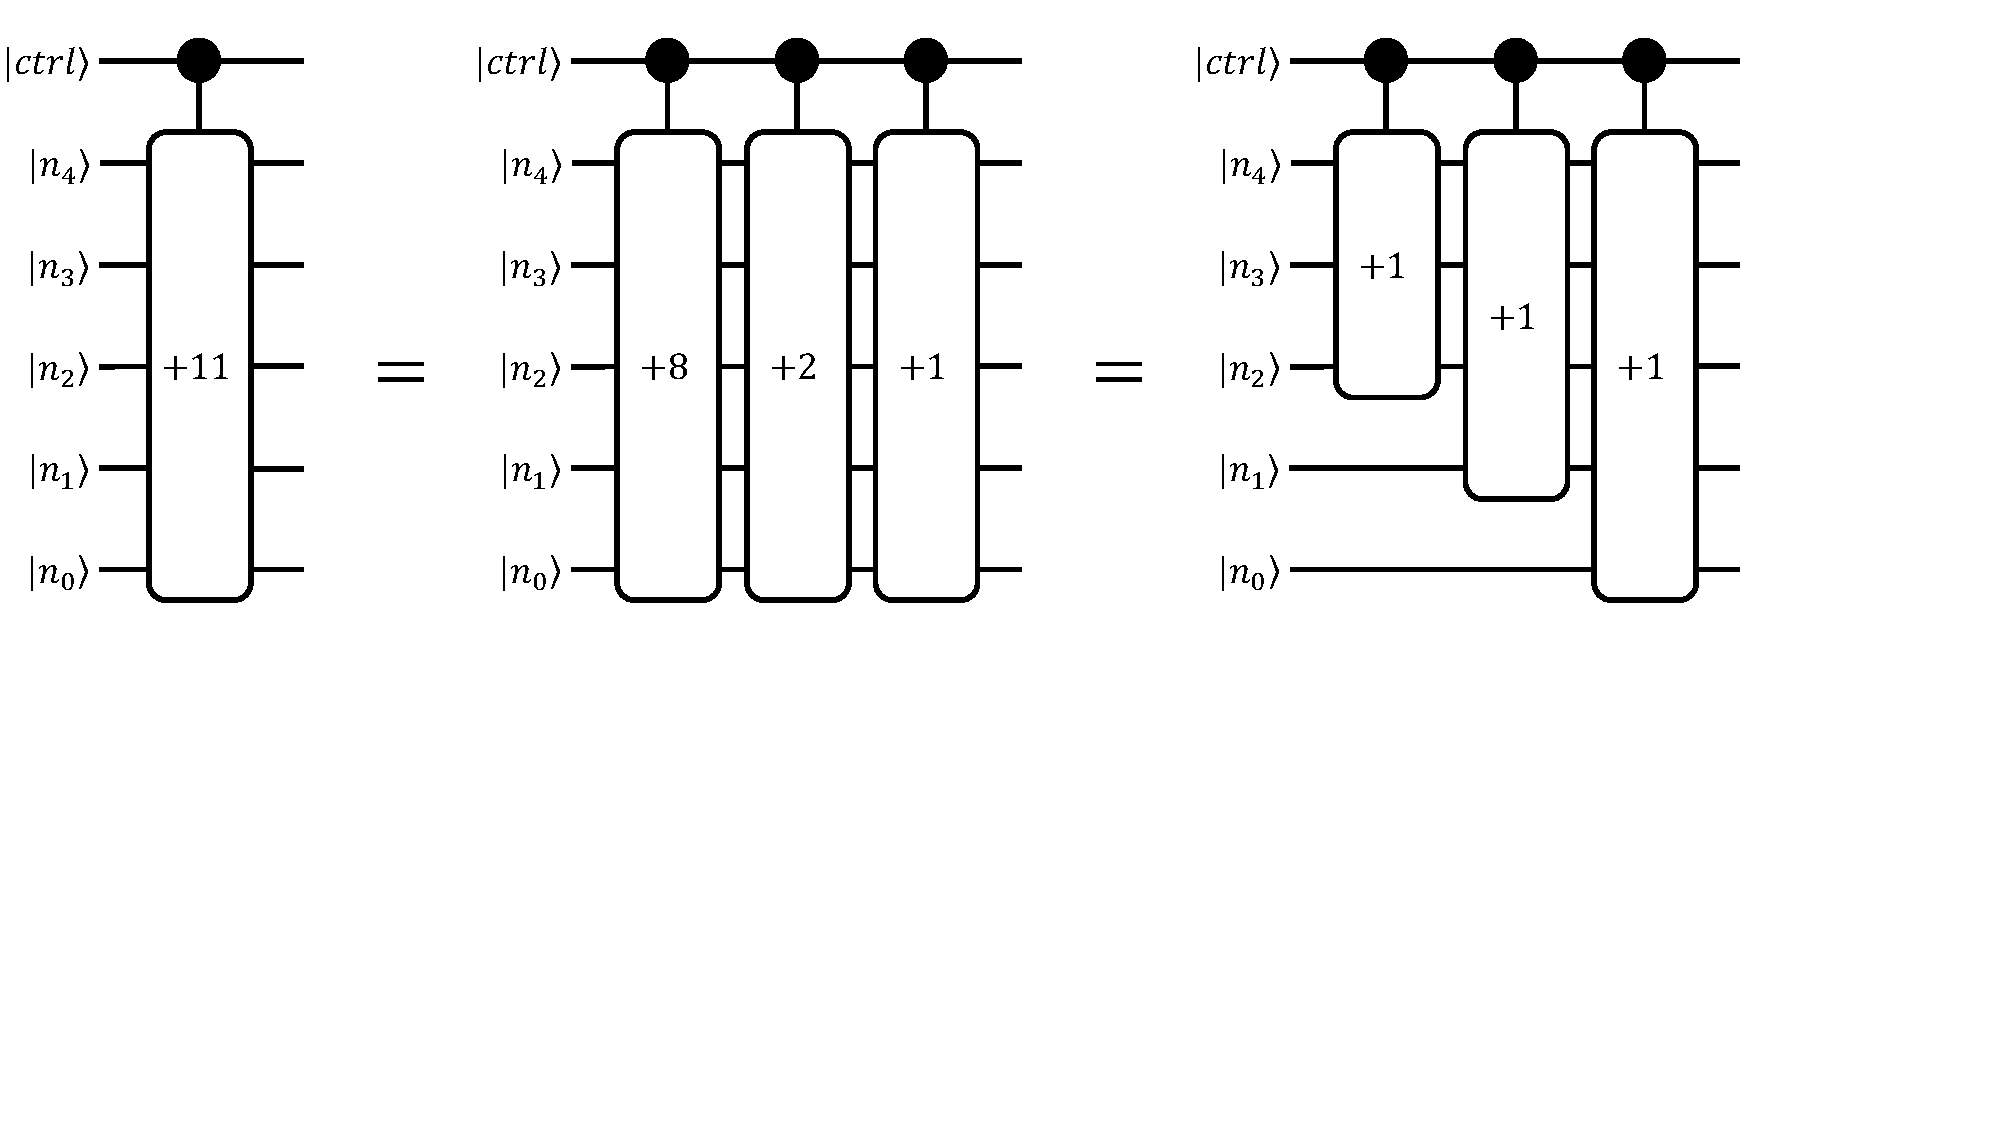
\includegraphics[width=16cm]{figures/addition-via-incrementers.pdf}
    \caption{
        \textbf{Addition via Controlled Incrementers.} 
    }
    \label{fig:addition-via-incrementers}
\end{figure}

\begin{figure}
    \centering
    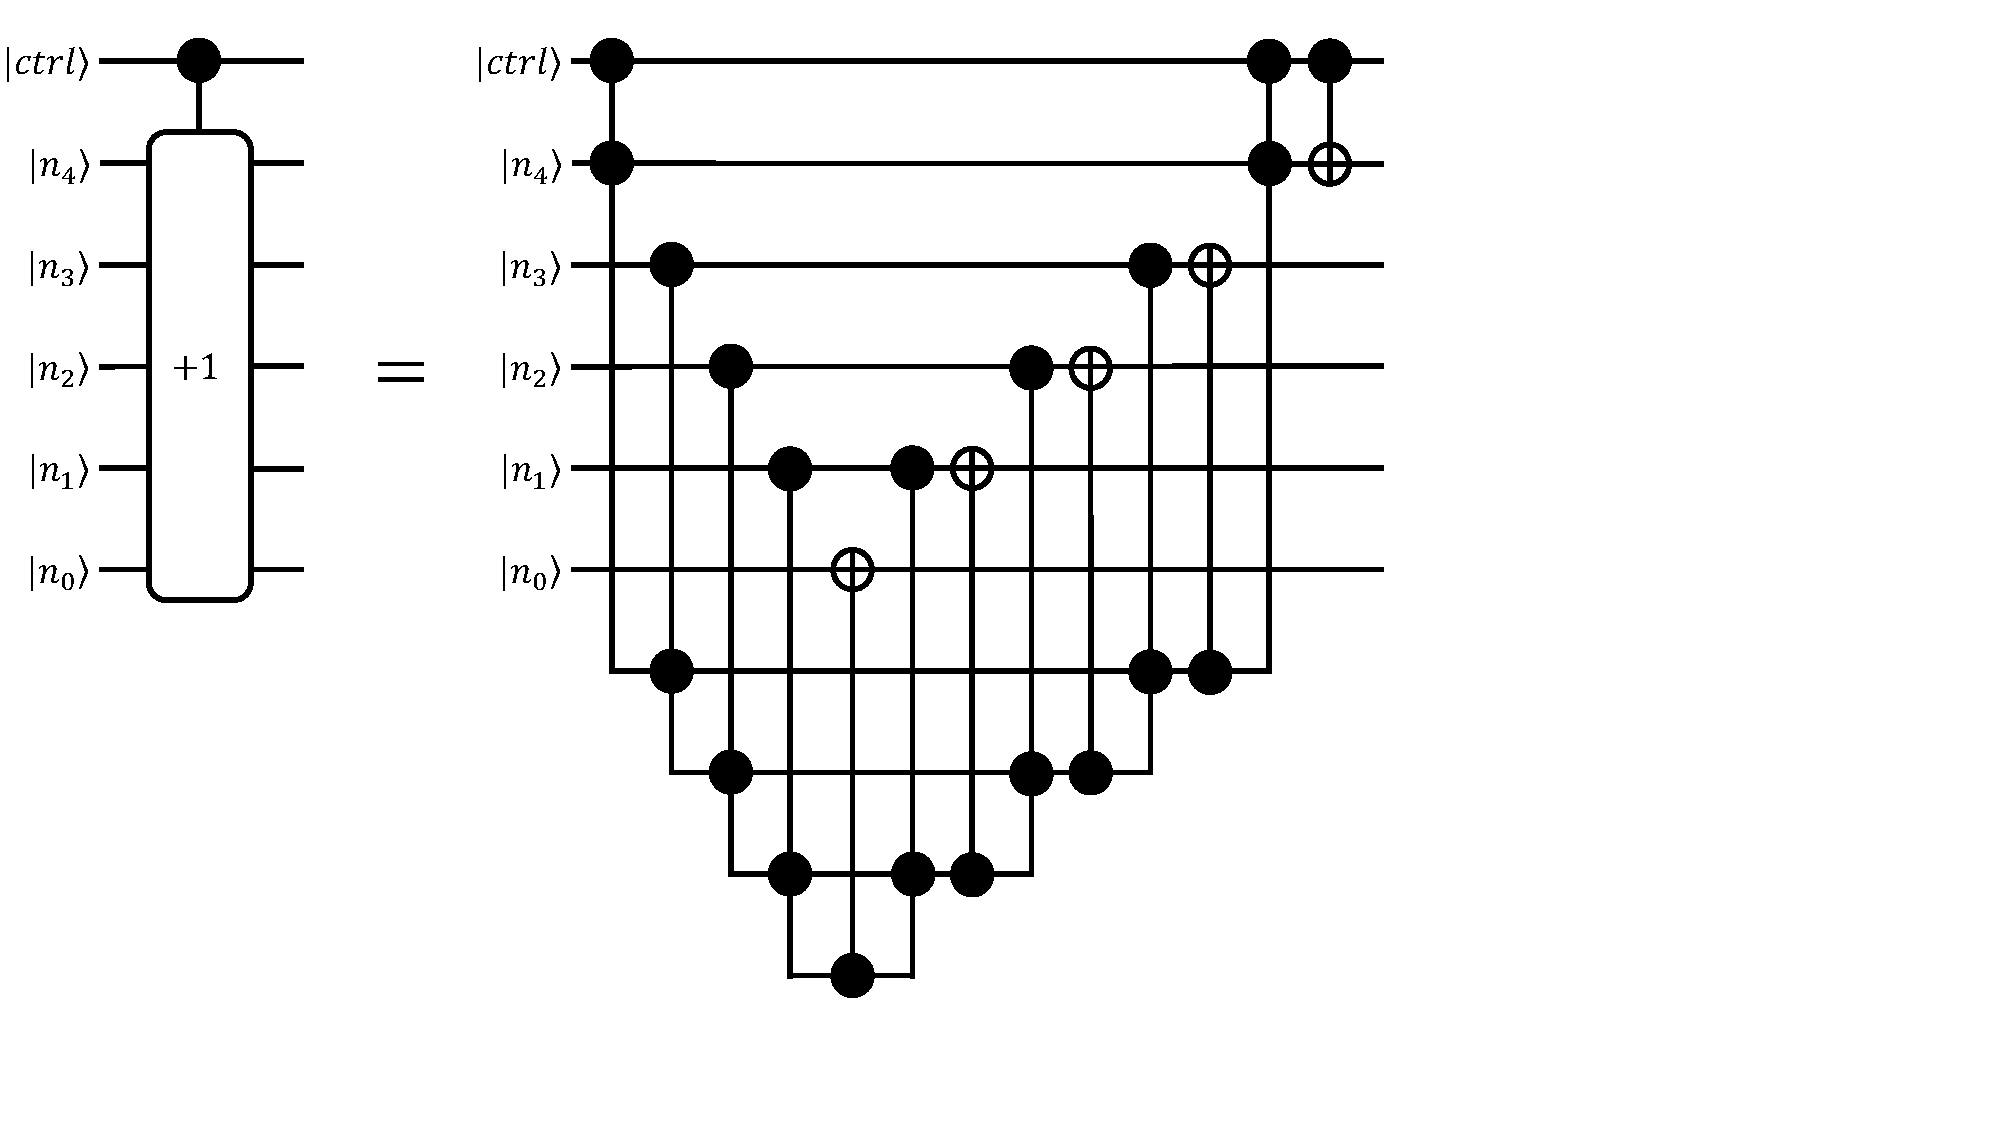
\includegraphics[width=8cm]{figures/incrementer.pdf}
    \caption{
        \textbf{Controlled Incrementer.} 
    }
    \label{fig:incrementer}
\end{figure}


One option is to use controlled incrementer ($+1$) circuits acting on different subsets of the register in order to construct the overall addition.
An incrementer circuit can be used to perform addition by a power of $2$ by shifting the qubits that the incrementer acts on.
For example, a circuit for adding the value $8$ to a register in binary can be performing using an incrementer circuit that treats the $4^{th}$ least significant qubit as the least significant qubit in the incrementer circuit and disregards the $3$ lesser qubits.
A circuit adding any classical value can then be constructed based on the binary representation of the classical number.
In Figure \ref{fig:addition-via-incrementers}, we show a quantum circuit diagram for adding the value $11$ to a quantum register using $3$ incrementer circuits adding the values $8$, $2$, and $1$. 
In Figure \ref{fig:incrementer} b, we decompose the incrementer circuit acting on a 5 qubit register using the construction detailed in \cite{Gidney_2015} which uses $N - 1$ left (and right) elbows and $N - 1$ ancillae.

Naively, the cost of this construction would require $N$ incrementer circuits which would each constribute a cost of $N - i - 1$ for $i \in [0, N-1)$ left (and right) elbows.
However, since we are performing modular addition, we an also achieve the same result by subtracting the value $2^N - m$.
The cost of these two methods can be classically determined and the more favorable option can be chosen during compilation.
If the number of left (and right) elbows is minimized, the upper bound for the number of left (and right) elbows, regardless of the classical value being added, is given by:
\begin{equation}
    \lfloor \frac{1}{4} N (N + 1) \rfloor = \lfloor \frac{1}{4} N^2 + \frac{1}{4} N \rfloor
\end{equation} 
\ws{this scaling was determined numerically, but i think it shouldn't be hard to derive.}

\begin{figure}
    \centering
    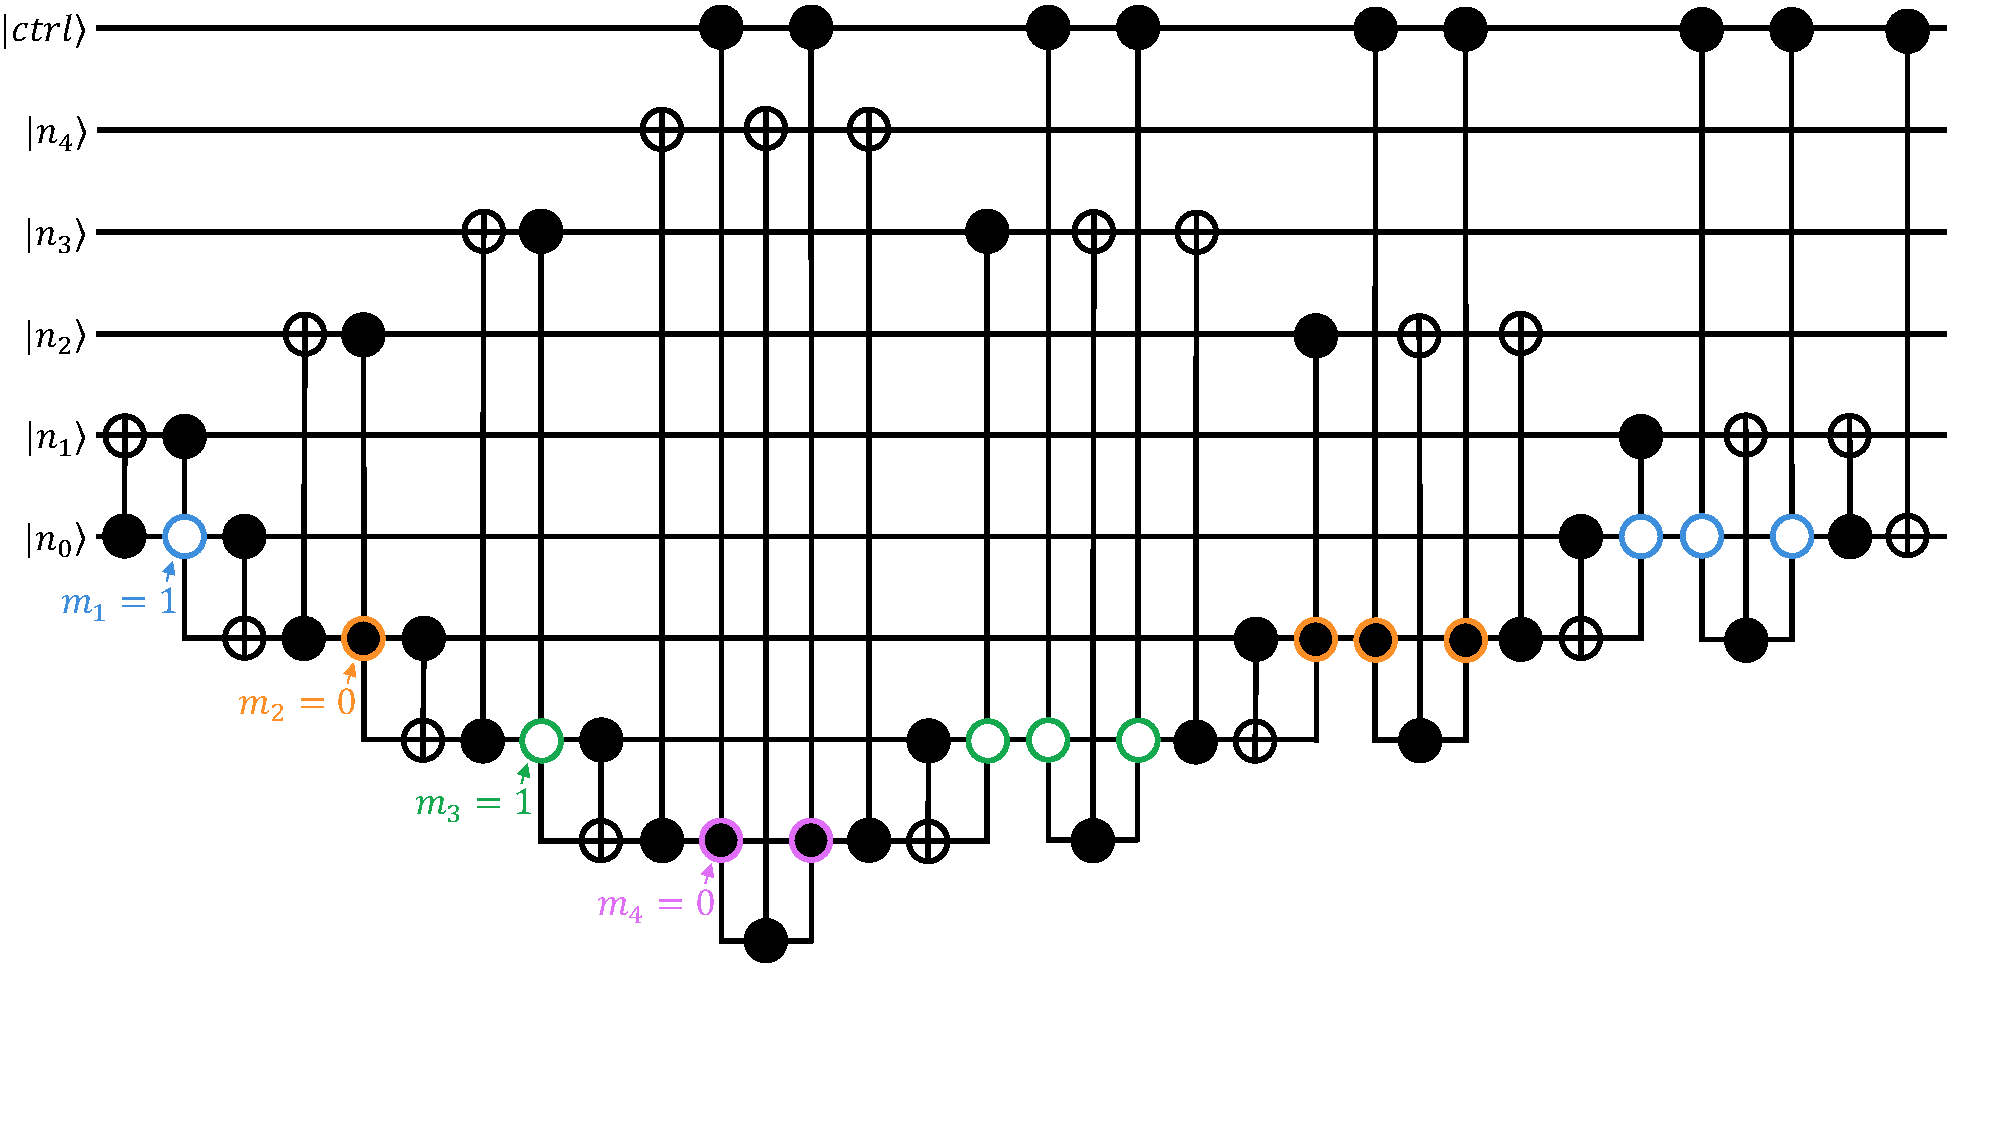
\includegraphics[width=12cm]{figures/ctrl-add-11-qubit-efficient.pdf}
    \caption{
        \textbf{Qubit Efficient Controlled Addition of 11.} 
    }
    \label{fig:addition-qubit-efficient-11}
\end{figure}

\begin{figure}
    \centering
    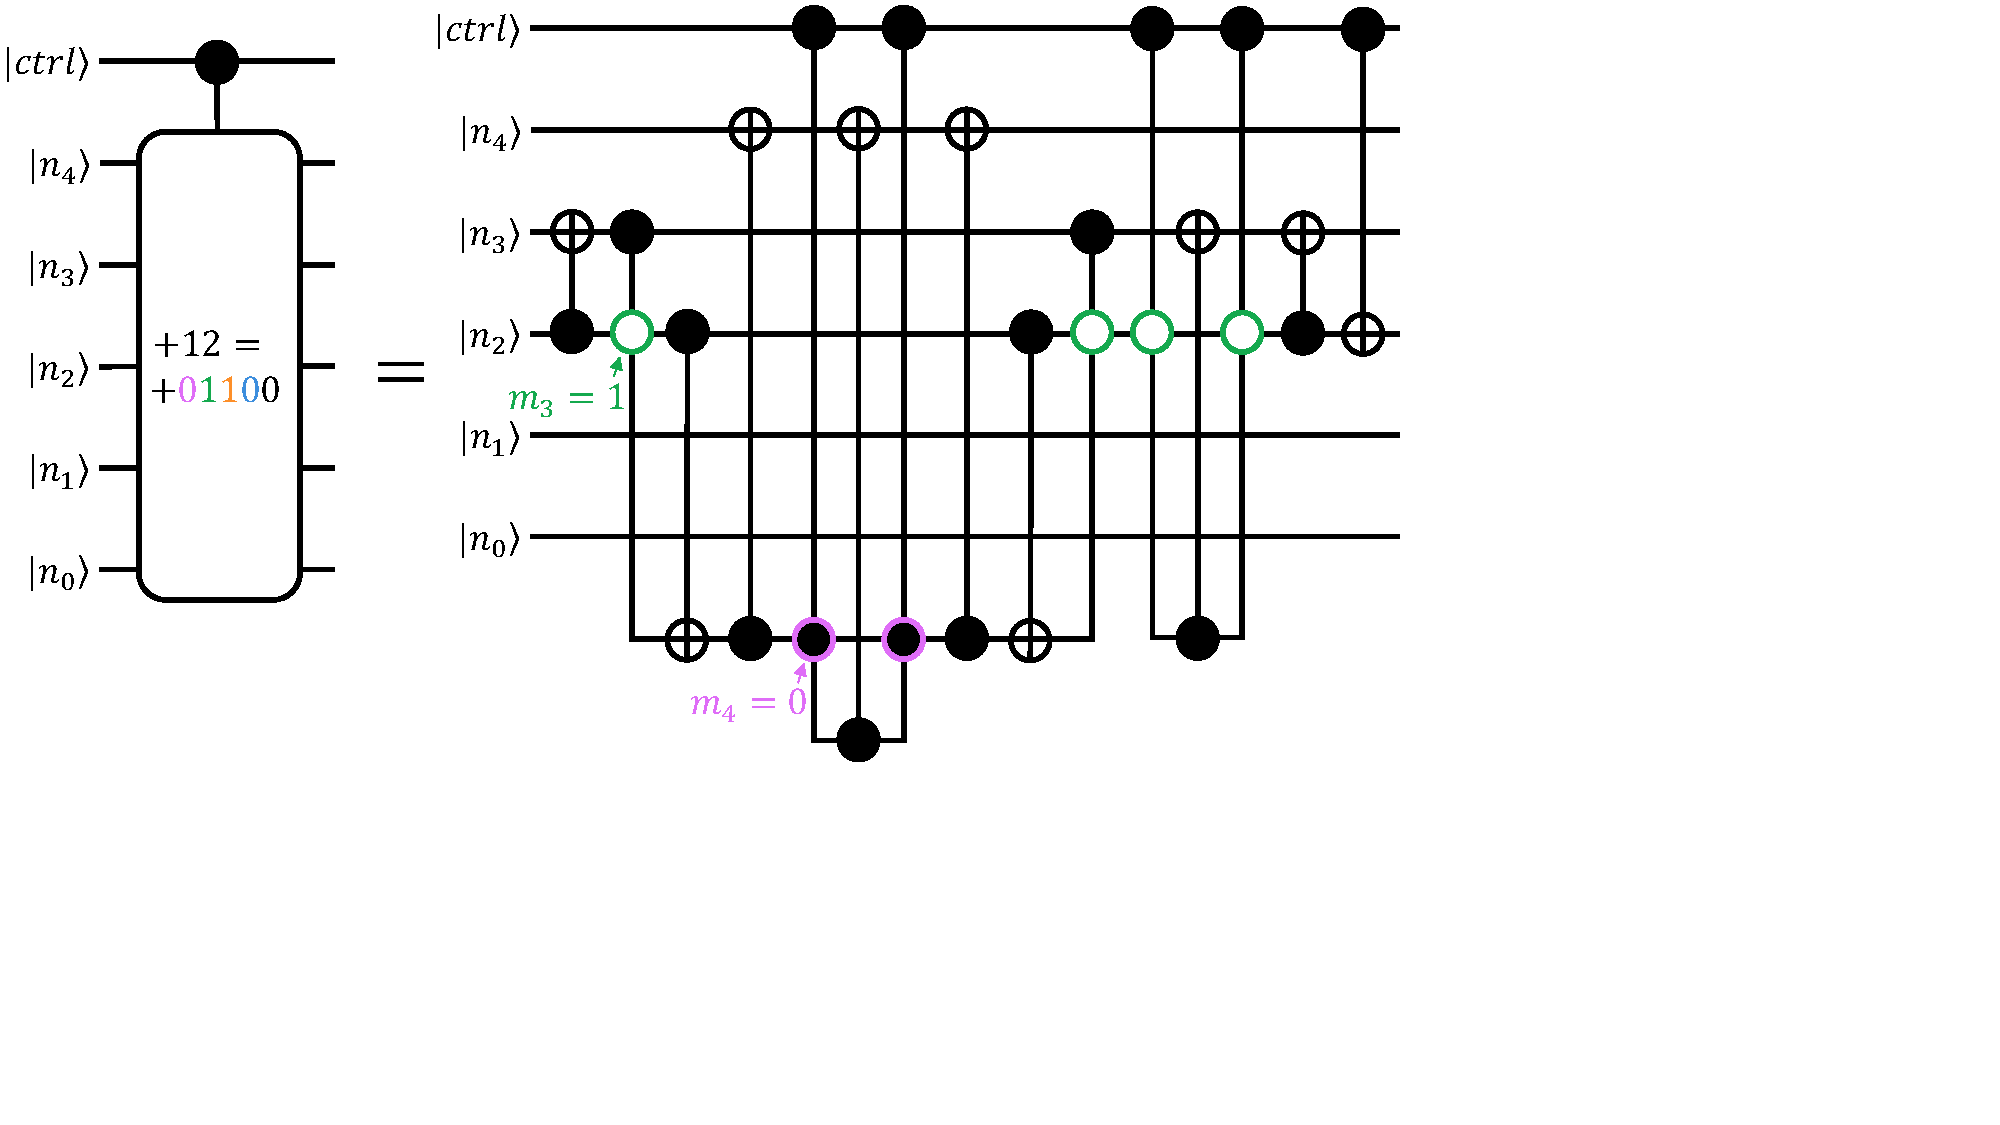
\includegraphics[width=8cm]{figures/ctrl-add-12-qubit-efficient.pdf}
    \caption{
        \textbf{Qubit Efficient Controlled Addition of 12.} 
    }
    \label{fig:addition-qubit-efficient-12}
\end{figure}

Another option is to use the same construction for the controlled quantum adder presented in \cite{gidney2018halving}, but to propagate the controls on the state of $\ket{m}$ into the circuit.
This method removes the register $\ket{m}$ from the quantum circuit, reducing the number of ancillae by $M$.
In Figure \ref{fig:addition-qubit-efficient-11}, we show a decomposition for this circuit when the number being added is $11$ ($01011$ in binary).
Additionally, since the lower bits of $m$ are known, the addition can be performed only beginning on the first non-zero bit of $m$.
An example of performing controlled addition of $12$ ($01100$ in binary) is shown in Figure \ref{fig:addition-qubit-efficient-12} where the $2$ least significant qubits are disregarded.
If the $p$ least significant bits of $m$ are zero, this reduces the cost to $2(N - p) - 3$ left (and right) elbows and $N - p - 1$ ancillae.

\begin{figure}
    \centering
    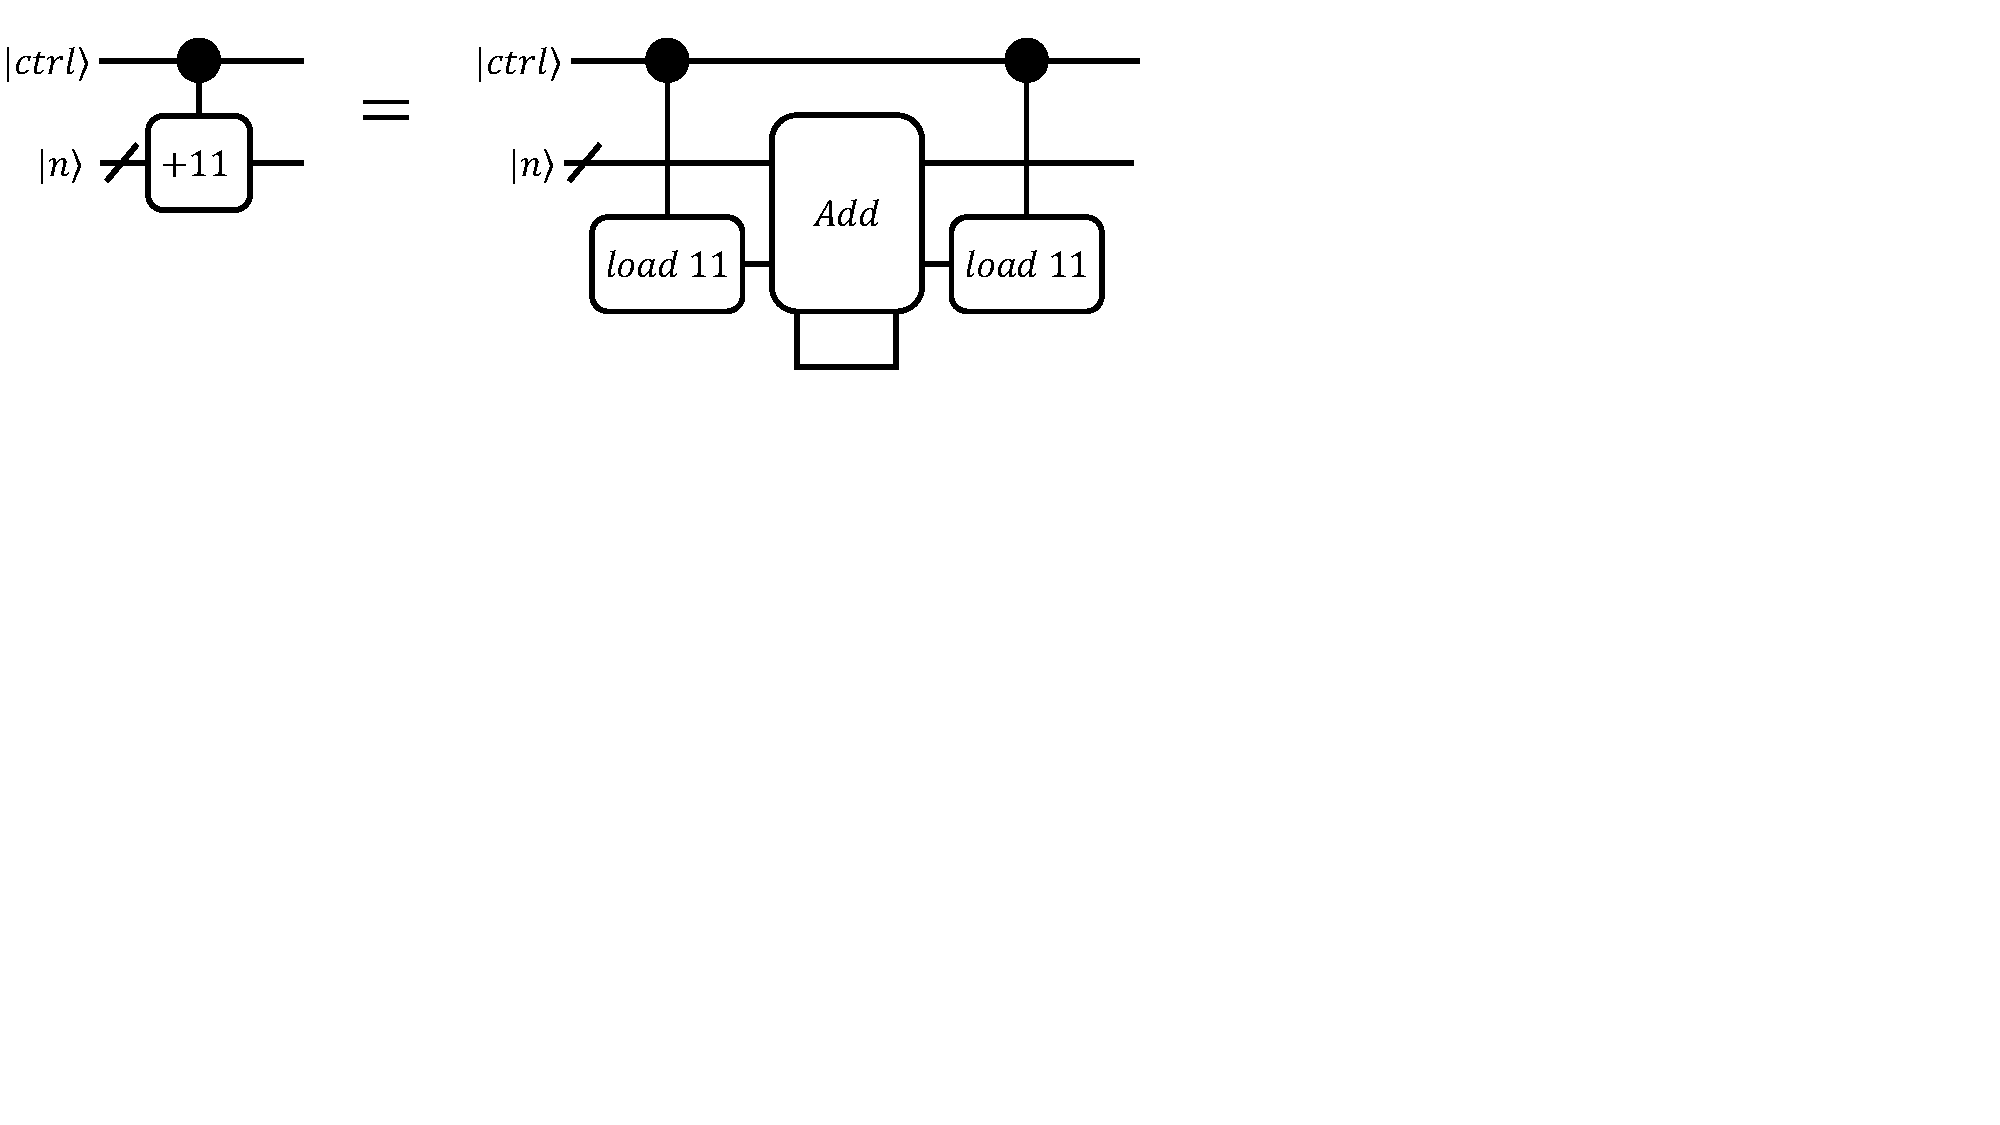
\includegraphics[width=12cm]{figures/ctrl-add-11-gate-efficient.pdf}
    \caption{
        \textbf{Gate Efficient Controlled Quantum Addition.} 
    }
    \label{fig:addition-gate-efficient}
\end{figure}

Lastly, a similar trick using the classical information about $m$ to modify the circuit for controlled addition shown in \cite{gidney2018halving} can reduce the number of left (and right) elbows.
In this construction, the value of $m$ is first loaded into a clean register using a series of CNOTs that are controlled on the control qubit.
The CNOTs present are determine from the binary decomposition of $m$.
Then an uncontrolled addition between the registers $\ket{m}$ and $\ket{n}$ can be performed using the decomposition in \cite{gidney2018halving}.
Finally, the controlled loading of $m$ is then performed again to uncompute the ancillae qubits and return them to a useable state.
A diagram of this ciruit is shown in Figure \ref{fig:addition-gate-efficient}.
Overall, this requires $N - p - 1$ left (and right) elbows and $N + M - p - 1$ ancillae.
Since this option requires the fewest non-Clifford operations while only using a moderate amount of ancillae, this option will be used to determine the resource estimates used in this work.
\section{Uniformly Controlled Rotations}
\label{sec:multiplexed-rotations}

Implementing a series of uniformly controlled rotations is a common subroutine used in this work.
In this section, we discuss the cost and explicit circuit compilation for a series of uniformly controlled rotations around the same axis (but different angles) are applied on the same qubit:
\begin{equation}
    \sum_{l=0}^{L - 1} \ket{l} \ket{\phi} \rightarrow \sum_{l=0}^{L - 1} \ket{l} R_a (\alpha_l) \ket{\phi}
\end{equation}

Möttönen et. al \cite{mottonen2004transformation}, provide a construction for \textit{uncontrolled} uniformly controlled rotations.
This construction is only defined when the number of rotations ($L$) is explicitly a power of $2$, however, if fewer rotations are required, then this can be achieved by padding with zero-angle rotations.

In this construction, the rotation angles are classically preprocessed based on the Gray code (Eq. 3 of \cite{mottonen2004transformation}):
\begin{equation}
    \begin{bmatrix}
        \theta_{0} \\
        \theta_{1} \\
        \vdots \\
        \theta_{L - 1}
    \end{bmatrix} = M \begin{bmatrix}
        \alpha_{0} \\
        \alpha_{1} \\
        \vdots \\
        \alpha_{L - 1}
    \end{bmatrix}
\end{equation}
where $M$ is a matrix transformation defined by:
\begin{equation}
    M_{i, j} = L^{-1} (-1)^{b_{j} . g_{i}}
\end{equation}
where $b_j$ is the binary representation of the integer $j$, $g_i$ is the Gray code representation of the integer $i$, and $b_{j} . g_{i}$ is the bitwise inner product of $b_{j}$ and $g_{i}$.

\begin{figure*}
    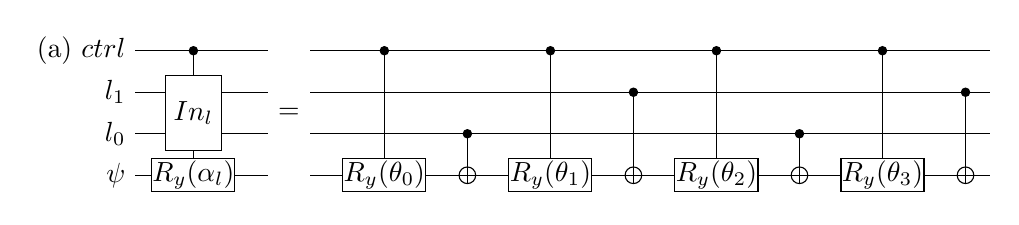
\begin{tikzpicture}[scale=1.000000,x=1pt,y=1pt]
\filldraw[color=white] (0.000000, -7.500000) rectangle (309.000000, 52.500000);
% Drawing wires
% Line 1: ctrl W \text{(a) }ctrl
\draw[color=black] (0.000000,45.000000) -- (309.000000,45.000000);
\draw[color=black] (0.000000,45.000000) node[left] {$\text{(a) }ctrl$};
% Line 2: l1 W l_1
\draw[color=black] (0.000000,30.000000) -- (309.000000,30.000000);
\draw[color=black] (0.000000,30.000000) node[left] {$l_1$};
% Line 3: l0 W l_0
\draw[color=black] (0.000000,15.000000) -- (309.000000,15.000000);
\draw[color=black] (0.000000,15.000000) node[left] {$l_0$};
% Line 4: sys W \psi
\draw[color=black] (0.000000,0.000000) -- (309.000000,0.000000);
\draw[color=black] (0.000000,0.000000) node[left] {$\psi$};
% Done with wires; drawing gates
% Line 6: l1 l0 G:width=20 $In_l$ sys G:width=30 $R_y (\alpha_l)$ ctrl
\draw (21.000000,45.000000) -- (21.000000,0.000000);
\begin{scope}
\draw[fill=white] (21.000000, 22.500000) +(-45.000000:14.142136pt and 19.091883pt) -- +(45.000000:14.142136pt and 19.091883pt) -- +(135.000000:14.142136pt and 19.091883pt) -- +(225.000000:14.142136pt and 19.091883pt) -- cycle;
\clip (21.000000, 22.500000) +(-45.000000:14.142136pt and 19.091883pt) -- +(45.000000:14.142136pt and 19.091883pt) -- +(135.000000:14.142136pt and 19.091883pt) -- +(225.000000:14.142136pt and 19.091883pt) -- cycle;
\draw (21.000000, 22.500000) node {$In_l$};
\end{scope}
\begin{scope}
\draw[fill=white] (21.000000, -0.000000) +(-45.000000:21.213203pt and 8.485281pt) -- +(45.000000:21.213203pt and 8.485281pt) -- +(135.000000:21.213203pt and 8.485281pt) -- +(225.000000:21.213203pt and 8.485281pt) -- cycle;
\clip (21.000000, -0.000000) +(-45.000000:21.213203pt and 8.485281pt) -- +(45.000000:21.213203pt and 8.485281pt) -- +(135.000000:21.213203pt and 8.485281pt) -- +(225.000000:21.213203pt and 8.485281pt) -- cycle;
\draw (21.000000, -0.000000) node {$R_y (\alpha_l)$};
\end{scope}
\filldraw (21.000000, 45.000000) circle(1.500000pt);
% Line 8: =
\draw[fill=white,color=white] (48.000000, -6.000000) rectangle (63.000000, 51.000000);
\draw (55.500000, 22.500000) node {$=$};
% Line 10: sys G width=30 $R_y (\theta_0)$ ctrl
\draw (90.000000,45.000000) -- (90.000000,0.000000);
\begin{scope}
\draw[fill=white] (90.000000, -0.000000) +(-45.000000:21.213203pt and 8.485281pt) -- +(45.000000:21.213203pt and 8.485281pt) -- +(135.000000:21.213203pt and 8.485281pt) -- +(225.000000:21.213203pt and 8.485281pt) -- cycle;
\clip (90.000000, -0.000000) +(-45.000000:21.213203pt and 8.485281pt) -- +(45.000000:21.213203pt and 8.485281pt) -- +(135.000000:21.213203pt and 8.485281pt) -- +(225.000000:21.213203pt and 8.485281pt) -- cycle;
\draw (90.000000, -0.000000) node {$R_y (\theta_0)$};
\end{scope}
\filldraw (90.000000, 45.000000) circle(1.500000pt);
% Line 11: +sys l0
\draw (120.000000,15.000000) -- (120.000000,0.000000);
\begin{scope}
\draw[fill=white] (120.000000, 0.000000) circle(3.000000pt);
\clip (120.000000, 0.000000) circle(3.000000pt);
\draw (117.000000, 0.000000) -- (123.000000, 0.000000);
\draw (120.000000, -3.000000) -- (120.000000, 3.000000);
\end{scope}
\filldraw (120.000000, 15.000000) circle(1.500000pt);
% Line 12: sys G width=30 $R_y (\theta_1)$ ctrl
\draw (150.000000,45.000000) -- (150.000000,0.000000);
\begin{scope}
\draw[fill=white] (150.000000, -0.000000) +(-45.000000:21.213203pt and 8.485281pt) -- +(45.000000:21.213203pt and 8.485281pt) -- +(135.000000:21.213203pt and 8.485281pt) -- +(225.000000:21.213203pt and 8.485281pt) -- cycle;
\clip (150.000000, -0.000000) +(-45.000000:21.213203pt and 8.485281pt) -- +(45.000000:21.213203pt and 8.485281pt) -- +(135.000000:21.213203pt and 8.485281pt) -- +(225.000000:21.213203pt and 8.485281pt) -- cycle;
\draw (150.000000, -0.000000) node {$R_y (\theta_1)$};
\end{scope}
\filldraw (150.000000, 45.000000) circle(1.500000pt);
% Line 13: +sys l1
\draw (180.000000,30.000000) -- (180.000000,0.000000);
\begin{scope}
\draw[fill=white] (180.000000, 0.000000) circle(3.000000pt);
\clip (180.000000, 0.000000) circle(3.000000pt);
\draw (177.000000, 0.000000) -- (183.000000, 0.000000);
\draw (180.000000, -3.000000) -- (180.000000, 3.000000);
\end{scope}
\filldraw (180.000000, 30.000000) circle(1.500000pt);
% Line 14: sys G width=30 $R_y (\theta_2)$ ctrl
\draw (210.000000,45.000000) -- (210.000000,0.000000);
\begin{scope}
\draw[fill=white] (210.000000, -0.000000) +(-45.000000:21.213203pt and 8.485281pt) -- +(45.000000:21.213203pt and 8.485281pt) -- +(135.000000:21.213203pt and 8.485281pt) -- +(225.000000:21.213203pt and 8.485281pt) -- cycle;
\clip (210.000000, -0.000000) +(-45.000000:21.213203pt and 8.485281pt) -- +(45.000000:21.213203pt and 8.485281pt) -- +(135.000000:21.213203pt and 8.485281pt) -- +(225.000000:21.213203pt and 8.485281pt) -- cycle;
\draw (210.000000, -0.000000) node {$R_y (\theta_2)$};
\end{scope}
\filldraw (210.000000, 45.000000) circle(1.500000pt);
% Line 15: +sys l0
\draw (240.000000,15.000000) -- (240.000000,0.000000);
\begin{scope}
\draw[fill=white] (240.000000, 0.000000) circle(3.000000pt);
\clip (240.000000, 0.000000) circle(3.000000pt);
\draw (237.000000, 0.000000) -- (243.000000, 0.000000);
\draw (240.000000, -3.000000) -- (240.000000, 3.000000);
\end{scope}
\filldraw (240.000000, 15.000000) circle(1.500000pt);
% Line 16: sys G width=30 $R_y (\theta_3)$ ctrl
\draw (270.000000,45.000000) -- (270.000000,0.000000);
\begin{scope}
\draw[fill=white] (270.000000, -0.000000) +(-45.000000:21.213203pt and 8.485281pt) -- +(45.000000:21.213203pt and 8.485281pt) -- +(135.000000:21.213203pt and 8.485281pt) -- +(225.000000:21.213203pt and 8.485281pt) -- cycle;
\clip (270.000000, -0.000000) +(-45.000000:21.213203pt and 8.485281pt) -- +(45.000000:21.213203pt and 8.485281pt) -- +(135.000000:21.213203pt and 8.485281pt) -- +(225.000000:21.213203pt and 8.485281pt) -- cycle;
\draw (270.000000, -0.000000) node {$R_y (\theta_3)$};
\end{scope}
\filldraw (270.000000, 45.000000) circle(1.500000pt);
% Line 17: +sys l1
\draw (300.000000,30.000000) -- (300.000000,0.000000);
\begin{scope}
\draw[fill=white] (300.000000, 0.000000) circle(3.000000pt);
\clip (300.000000, 0.000000) circle(3.000000pt);
\draw (297.000000, 0.000000) -- (303.000000, 0.000000);
\draw (300.000000, -3.000000) -- (300.000000, 3.000000);
\end{scope}
\filldraw (300.000000, 30.000000) circle(1.500000pt);
% Done with gates; drawing ending labels
% Done with ending labels; drawing cut lines and comments
% Done with comments
\end{tikzpicture}

    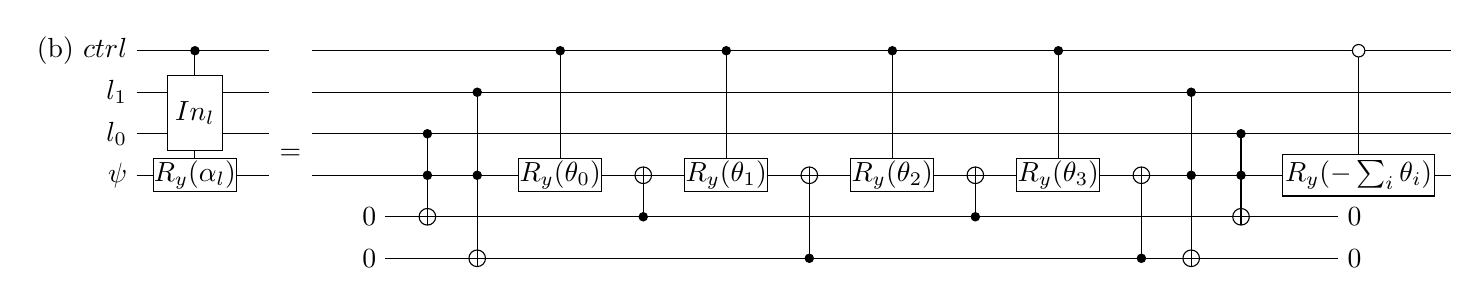
\begin{tikzpicture}[scale=1.000000,x=1pt,y=1pt]
\filldraw[color=white] (0.000000, -7.500000) rectangle (475.000000, 82.500000);
% Drawing wires
% Line 1: ctrl W \text{(b) }ctrl
\draw[color=black] (0.000000,75.000000) -- (475.000000,75.000000);
\draw[color=black] (0.000000,75.000000) node[left] {$\text{(b) }ctrl$};
% Line 2: l1 W l_1
\draw[color=black] (0.000000,60.000000) -- (475.000000,60.000000);
\draw[color=black] (0.000000,60.000000) node[left] {$l_1$};
% Line 3: l0 W l_0
\draw[color=black] (0.000000,45.000000) -- (475.000000,45.000000);
\draw[color=black] (0.000000,45.000000) node[left] {$l_0$};
% Line 4: sys W \psi
\draw[color=black] (0.000000,30.000000) -- (475.000000,30.000000);
\draw[color=black] (0.000000,30.000000) node[left] {$\psi$};
% Line 5: c0 W 0 0
\draw[color=black] (82.500000,15.000000) -- (441.500000,15.000000);
% Line 6: c1 W 0 0
\draw[color=black] (82.500000,0.000000) -- (441.500000,0.000000);
% Done with wires; drawing gates
% Line 8: sys G:width=30 $R_y (\alpha_l)$ l1 l0 G:width=20 $In_l$ ctrl
\draw (21.000000,75.000000) -- (21.000000,30.000000);
\begin{scope}
\draw[fill=white] (21.000000, 30.000000) +(-45.000000:21.213203pt and 8.485281pt) -- +(45.000000:21.213203pt and 8.485281pt) -- +(135.000000:21.213203pt and 8.485281pt) -- +(225.000000:21.213203pt and 8.485281pt) -- cycle;
\clip (21.000000, 30.000000) +(-45.000000:21.213203pt and 8.485281pt) -- +(45.000000:21.213203pt and 8.485281pt) -- +(135.000000:21.213203pt and 8.485281pt) -- +(225.000000:21.213203pt and 8.485281pt) -- cycle;
\draw (21.000000, 30.000000) node {$R_y (\alpha_l)$};
\end{scope}
\begin{scope}
\draw[fill=white] (21.000000, 52.500000) +(-45.000000:14.142136pt and 19.091883pt) -- +(45.000000:14.142136pt and 19.091883pt) -- +(135.000000:14.142136pt and 19.091883pt) -- +(225.000000:14.142136pt and 19.091883pt) -- cycle;
\clip (21.000000, 52.500000) +(-45.000000:14.142136pt and 19.091883pt) -- +(45.000000:14.142136pt and 19.091883pt) -- +(135.000000:14.142136pt and 19.091883pt) -- +(225.000000:14.142136pt and 19.091883pt) -- cycle;
\draw (21.000000, 52.500000) node {$In_l$};
\end{scope}
\filldraw (21.000000, 75.000000) circle(1.500000pt);
% Line 10: =
\draw[fill=white,color=white] (48.000000, -6.000000) rectangle (63.000000, 81.000000);
\draw (55.500000, 37.500000) node {$=$};
% Line 12: c0 c1 START
\draw[color=black] (90.000000,15.000000) node[fill=white,left,minimum height=15.000000pt,minimum width=15.000000pt,inner sep=0pt] {\phantom{$0$}};
\draw[color=black] (90.000000,15.000000) node[left] {$0$};
\draw[color=black] (90.000000,0.000000) node[fill=white,left,minimum height=15.000000pt,minimum width=15.000000pt,inner sep=0pt] {\phantom{$0$}};
\draw[color=black] (90.000000,0.000000) node[left] {$0$};
% Line 13: +c0 sys l0
\draw (105.000000,45.000000) -- (105.000000,15.000000);
\begin{scope}
\draw[fill=white] (105.000000, 15.000000) circle(3.000000pt);
\clip (105.000000, 15.000000) circle(3.000000pt);
\draw (102.000000, 15.000000) -- (108.000000, 15.000000);
\draw (105.000000, 12.000000) -- (105.000000, 18.000000);
\end{scope}
\filldraw (105.000000, 30.000000) circle(1.500000pt);
\filldraw (105.000000, 45.000000) circle(1.500000pt);
% Line 14: +c1 sys l1
\draw (123.000000,60.000000) -- (123.000000,0.000000);
\begin{scope}
\draw[fill=white] (123.000000, 0.000000) circle(3.000000pt);
\clip (123.000000, 0.000000) circle(3.000000pt);
\draw (120.000000, 0.000000) -- (126.000000, 0.000000);
\draw (123.000000, -3.000000) -- (123.000000, 3.000000);
\end{scope}
\filldraw (123.000000, 30.000000) circle(1.500000pt);
\filldraw (123.000000, 60.000000) circle(1.500000pt);
% Line 16: sys G width=30 $R_y (\theta_0)$ ctrl
\draw (153.000000,75.000000) -- (153.000000,30.000000);
\begin{scope}
\draw[fill=white] (153.000000, 30.000000) +(-45.000000:21.213203pt and 8.485281pt) -- +(45.000000:21.213203pt and 8.485281pt) -- +(135.000000:21.213203pt and 8.485281pt) -- +(225.000000:21.213203pt and 8.485281pt) -- cycle;
\clip (153.000000, 30.000000) +(-45.000000:21.213203pt and 8.485281pt) -- +(45.000000:21.213203pt and 8.485281pt) -- +(135.000000:21.213203pt and 8.485281pt) -- +(225.000000:21.213203pt and 8.485281pt) -- cycle;
\draw (153.000000, 30.000000) node {$R_y (\theta_0)$};
\end{scope}
\filldraw (153.000000, 75.000000) circle(1.500000pt);
% Line 17: +sys c0
\draw (183.000000,30.000000) -- (183.000000,15.000000);
\begin{scope}
\draw[fill=white] (183.000000, 30.000000) circle(3.000000pt);
\clip (183.000000, 30.000000) circle(3.000000pt);
\draw (180.000000, 30.000000) -- (186.000000, 30.000000);
\draw (183.000000, 27.000000) -- (183.000000, 33.000000);
\end{scope}
\filldraw (183.000000, 15.000000) circle(1.500000pt);
% Line 18: sys G width=30 $R_y (\theta_1)$ ctrl
\draw (213.000000,75.000000) -- (213.000000,30.000000);
\begin{scope}
\draw[fill=white] (213.000000, 30.000000) +(-45.000000:21.213203pt and 8.485281pt) -- +(45.000000:21.213203pt and 8.485281pt) -- +(135.000000:21.213203pt and 8.485281pt) -- +(225.000000:21.213203pt and 8.485281pt) -- cycle;
\clip (213.000000, 30.000000) +(-45.000000:21.213203pt and 8.485281pt) -- +(45.000000:21.213203pt and 8.485281pt) -- +(135.000000:21.213203pt and 8.485281pt) -- +(225.000000:21.213203pt and 8.485281pt) -- cycle;
\draw (213.000000, 30.000000) node {$R_y (\theta_1)$};
\end{scope}
\filldraw (213.000000, 75.000000) circle(1.500000pt);
% Line 19: +sys c1
\draw (243.000000,30.000000) -- (243.000000,0.000000);
\begin{scope}
\draw[fill=white] (243.000000, 30.000000) circle(3.000000pt);
\clip (243.000000, 30.000000) circle(3.000000pt);
\draw (240.000000, 30.000000) -- (246.000000, 30.000000);
\draw (243.000000, 27.000000) -- (243.000000, 33.000000);
\end{scope}
\filldraw (243.000000, 0.000000) circle(1.500000pt);
% Line 20: sys G width=30 $R_y (\theta_2)$ ctrl
\draw (273.000000,75.000000) -- (273.000000,30.000000);
\begin{scope}
\draw[fill=white] (273.000000, 30.000000) +(-45.000000:21.213203pt and 8.485281pt) -- +(45.000000:21.213203pt and 8.485281pt) -- +(135.000000:21.213203pt and 8.485281pt) -- +(225.000000:21.213203pt and 8.485281pt) -- cycle;
\clip (273.000000, 30.000000) +(-45.000000:21.213203pt and 8.485281pt) -- +(45.000000:21.213203pt and 8.485281pt) -- +(135.000000:21.213203pt and 8.485281pt) -- +(225.000000:21.213203pt and 8.485281pt) -- cycle;
\draw (273.000000, 30.000000) node {$R_y (\theta_2)$};
\end{scope}
\filldraw (273.000000, 75.000000) circle(1.500000pt);
% Line 21: +sys c0
\draw (303.000000,30.000000) -- (303.000000,15.000000);
\begin{scope}
\draw[fill=white] (303.000000, 30.000000) circle(3.000000pt);
\clip (303.000000, 30.000000) circle(3.000000pt);
\draw (300.000000, 30.000000) -- (306.000000, 30.000000);
\draw (303.000000, 27.000000) -- (303.000000, 33.000000);
\end{scope}
\filldraw (303.000000, 15.000000) circle(1.500000pt);
% Line 22: sys G width=30 $R_y (\theta_3)$ ctrl
\draw (333.000000,75.000000) -- (333.000000,30.000000);
\begin{scope}
\draw[fill=white] (333.000000, 30.000000) +(-45.000000:21.213203pt and 8.485281pt) -- +(45.000000:21.213203pt and 8.485281pt) -- +(135.000000:21.213203pt and 8.485281pt) -- +(225.000000:21.213203pt and 8.485281pt) -- cycle;
\clip (333.000000, 30.000000) +(-45.000000:21.213203pt and 8.485281pt) -- +(45.000000:21.213203pt and 8.485281pt) -- +(135.000000:21.213203pt and 8.485281pt) -- +(225.000000:21.213203pt and 8.485281pt) -- cycle;
\draw (333.000000, 30.000000) node {$R_y (\theta_3)$};
\end{scope}
\filldraw (333.000000, 75.000000) circle(1.500000pt);
% Line 23: +sys c1
\draw (363.000000,30.000000) -- (363.000000,0.000000);
\begin{scope}
\draw[fill=white] (363.000000, 30.000000) circle(3.000000pt);
\clip (363.000000, 30.000000) circle(3.000000pt);
\draw (360.000000, 30.000000) -- (366.000000, 30.000000);
\draw (363.000000, 27.000000) -- (363.000000, 33.000000);
\end{scope}
\filldraw (363.000000, 0.000000) circle(1.500000pt);
% Line 25: +c1 sys l1
\draw (381.000000,60.000000) -- (381.000000,0.000000);
\begin{scope}
\draw[fill=white] (381.000000, 0.000000) circle(3.000000pt);
\clip (381.000000, 0.000000) circle(3.000000pt);
\draw (378.000000, 0.000000) -- (384.000000, 0.000000);
\draw (381.000000, -3.000000) -- (381.000000, 3.000000);
\end{scope}
\filldraw (381.000000, 30.000000) circle(1.500000pt);
\filldraw (381.000000, 60.000000) circle(1.500000pt);
% Line 26: +c0 sys l0
\draw (399.000000,45.000000) -- (399.000000,15.000000);
\begin{scope}
\draw[fill=white] (399.000000, 15.000000) circle(3.000000pt);
\clip (399.000000, 15.000000) circle(3.000000pt);
\draw (396.000000, 15.000000) -- (402.000000, 15.000000);
\draw (399.000000, 12.000000) -- (399.000000, 18.000000);
\end{scope}
\filldraw (399.000000, 30.000000) circle(1.500000pt);
\filldraw (399.000000, 45.000000) circle(1.500000pt);
% Line 27: c0 c1 END
\draw[color=black] (434.000000,15.000000) node[fill=white,right,minimum height=15.000000pt,minimum width=15.000000pt,inner sep=0pt] {\phantom{$0$}};
\draw[color=black] (434.000000,15.000000) node[right] {$0$};
\draw[color=black] (434.000000,0.000000) node[fill=white,right,minimum height=15.000000pt,minimum width=15.000000pt,inner sep=0pt] {\phantom{$0$}};
\draw[color=black] (434.000000,0.000000) node[right] {$0$};
% Line 29: sys G:width=55:height=15 $R_y(-\sum_i \theta_i)$ -ctrl
\draw (441.500000,75.000000) -- (441.500000,30.000000);
\begin{scope}
\draw[fill=white] (441.500000, 30.000000) +(-45.000000:38.890873pt and 10.606602pt) -- +(45.000000:38.890873pt and 10.606602pt) -- +(135.000000:38.890873pt and 10.606602pt) -- +(225.000000:38.890873pt and 10.606602pt) -- cycle;
\clip (441.500000, 30.000000) +(-45.000000:38.890873pt and 10.606602pt) -- +(45.000000:38.890873pt and 10.606602pt) -- +(135.000000:38.890873pt and 10.606602pt) -- +(225.000000:38.890873pt and 10.606602pt) -- cycle;
\draw (441.500000, 30.000000) node {$R_y(-\sum_i \theta_i)$};
\end{scope}
\draw[fill=white] (441.500000, 75.000000) circle(2.250000pt);
% Done with gates; drawing ending labels
% Done with ending labels; drawing cut lines and comments
% Done with comments
\end{tikzpicture}

    \caption{
        \textbf{Controlled Uniformly Controlled Rotations}
        Two implementations for controlling a series of uniformly controlled rotations are shown.
        In (a), a naive implementation is shown which doubles the number of arbitrary rotations required.
        The implementation shown in (b) uses only one additional controlled rotation and $\log_2 L$ Toffoli gates, but requires $\log_2 L$ clean ancillae.
    }
    \label{fig:controlled-multiplexed-rotations}
\end{figure*}

However, in this work we require the use of a \textit{controlled} series of uniformly controlled rotations.
Naively, this can be implemented by controlling each of the arbitrary rotations in the construction given by Möttönen et al. \cite{mottonen2004transformation}.
An example circuit diagram for this construction is shown in subfigure \ref{fig:controlled-multiplexed-rotations}a.
Since each controlled rotation can be implemented by two uncontrolled rotations, this compilation strategy uses $2L$ uncontrolled arbitrary rotations.

An alternative approach which uses $4 \log_2 L$ T gates, $L + 3$ arbitrary rotations, and $\log_2 L$ clean ancillae is shown in subfigure \ref{fig:controlled-multiplexed-rotations}b.
In this construction, the temporary logical-AND of each qubit in the index register and the control qubit is computed using $\log_2 L$ Toffoli gates.
CNOTs from these clean ancillae then conjugate each of the arbitrary rotations which are left uncontrolled.
When the control is on, this fully recovers the construction given by Möttönen et. al.

However, when the control is off, the uncontrolled arbitrary rotations are still applied, resulting an undesired rotation of angle $\sum_{i} (\theta_i)$.
This undesired rotation can then be undone using one $0$-controlled rotation of angle $- \sum_{i} (\theta_i)$.

\section{Grover-Rudolph State Preparation}
\label{sec:grover-rudolph}

In this section, we will describe the Grover-Rudolph state-preparation routine \cite{grover2002creating} in the context that it is used in this work.
The Grover-Rudolph state-preparation algorithm constructs quantum circuits that prepare states of the form given by:
\begin{equation}
    \ket{0^{\otimes \lceil \log_2{L} \rceil}} \rightarrow_{\textit{Grover-Rudolph}} \sum_{l=0}^L \sqrt{p(l)} \ket{l}
\end{equation}
where $p(l)$ is a probability distribution along the different indices ($l$) with the constraint that $\sum_l p(l) = 1$.

In the context of block-encodings, preparing such probability distributions can be used to construct the $Prepare$ oracle (Eq. \ref{eq:prep-state}).
The probability distribution in this case is defined by the normalized magnitudes of the coefficients of the terms in the linear combination: $p(l) = |\alpha_l| / \lambda$.

The Grover-Rudolph algorithm works by sequentially summing up the probability distribution to the left and right of a given index and then performing a rotation controlled on the current index.

For example, given the (noramlized) probabilities $\alpha_0$, $\alpha_1$, $\alpha_2$, and $\alpha_3$, the Grover-Rudolph algorithm proceeds as follows:
\begin{enumerate}
    \item Perform a Pauli-Y rotation on the top (left-most) qubit in the register by an angle: $\theta = 2 \cos^{-1}\big( \sqrt{\alpha_0 + \alpha_1} \big)$.
    \item Perform a Pauli-Y rotation on the second qubit in the register, controlled on the first qubit being in the state $\ket{0}$ by an angle: $\theta = 2 \cos^{-1}\big( \sqrt{\frac{\alpha_0}{\alpha_0 + \alpha_1}} \big)$
    \item Perform a Pauli-Y rotation on the second qubit in the register, controlled on the first qubit being in the state $\ket{1}$ by an angle: $\theta = 2 \cos^{-1}\big( \sqrt{\frac{\alpha_2}{\alpha_2 + \alpha_3}} \big)$
\end{enumerate}

The evolution of the quantum state is given by:
\begin{equation}
    \begin{split}
        \ket{00} &\rightarrow_{\textit{(i)}} \sqrt{\alpha_0 + \alpha_1} \ket{00} + \sqrt{\alpha_2 + \alpha_3} \ket{10} \\
        &\rightarrow_{\textit{(ii)}} \sqrt{\alpha_0} \ket{00} + \sqrt{\alpha_1} \ket{01} + \sqrt{\alpha_2 + \alpha_3} \ket{10} \\
        &\rightarrow_{\textit{(iii)}} \sqrt{\alpha_0} \ket{00} + \sqrt{\alpha_1} \ket{01} + \alpha_2 \ket{10} + \alpha_3 \ket{11}
    \end{split}
\end{equation}

\begin{figure*}
    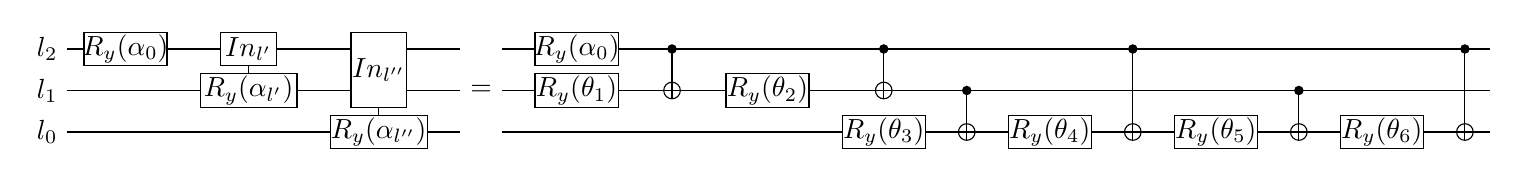
\begin{tikzpicture}[scale=1.000000,x=1pt,y=1pt]
\filldraw[color=white] (0.000000, -7.500000) rectangle (514.000000, 37.500000);
% Drawing wires
% Line 1: l2 W l_2
\draw[color=black] (0.000000,30.000000) -- (514.000000,30.000000);
\draw[color=black] (0.000000,30.000000) node[left] {$l_2$};
% Line 2: l1 W l_1
\draw[color=black] (0.000000,15.000000) -- (514.000000,15.000000);
\draw[color=black] (0.000000,15.000000) node[left] {$l_1$};
% Line 3: l0 W l_0
\draw[color=black] (0.000000,0.000000) -- (514.000000,0.000000);
\draw[color=black] (0.000000,0.000000) node[left] {$l_0$};
% Done with wires; drawing gates
% Line 5: l2 G:width=30 $R_y (\alpha_0)$
\begin{scope}
\draw[fill=white] (21.000000, 30.000000) +(-45.000000:21.213203pt and 8.485281pt) -- +(45.000000:21.213203pt and 8.485281pt) -- +(135.000000:21.213203pt and 8.485281pt) -- +(225.000000:21.213203pt and 8.485281pt) -- cycle;
\clip (21.000000, 30.000000) +(-45.000000:21.213203pt and 8.485281pt) -- +(45.000000:21.213203pt and 8.485281pt) -- +(135.000000:21.213203pt and 8.485281pt) -- +(225.000000:21.213203pt and 8.485281pt) -- cycle;
\draw (21.000000, 30.000000) node {$R_y (\alpha_0)$};
\end{scope}
% Line 6: l1 G:width=35 $R_y (\alpha_{l^\prime})$ l2 G:width=20 $In_{l^\prime}$
\draw (65.500000,30.000000) -- (65.500000,15.000000);
\begin{scope}
\draw[fill=white] (65.500000, 15.000000) +(-45.000000:24.748737pt and 8.485281pt) -- +(45.000000:24.748737pt and 8.485281pt) -- +(135.000000:24.748737pt and 8.485281pt) -- +(225.000000:24.748737pt and 8.485281pt) -- cycle;
\clip (65.500000, 15.000000) +(-45.000000:24.748737pt and 8.485281pt) -- +(45.000000:24.748737pt and 8.485281pt) -- +(135.000000:24.748737pt and 8.485281pt) -- +(225.000000:24.748737pt and 8.485281pt) -- cycle;
\draw (65.500000, 15.000000) node {$R_y (\alpha_{l^\prime})$};
\end{scope}
\begin{scope}
\draw[fill=white] (65.500000, 30.000000) +(-45.000000:14.142136pt and 8.485281pt) -- +(45.000000:14.142136pt and 8.485281pt) -- +(135.000000:14.142136pt and 8.485281pt) -- +(225.000000:14.142136pt and 8.485281pt) -- cycle;
\clip (65.500000, 30.000000) +(-45.000000:14.142136pt and 8.485281pt) -- +(45.000000:14.142136pt and 8.485281pt) -- +(135.000000:14.142136pt and 8.485281pt) -- +(225.000000:14.142136pt and 8.485281pt) -- cycle;
\draw (65.500000, 30.000000) node {$In_{l^\prime}$};
\end{scope}
% Line 7: l0 G:width=35 $R_y (\alpha_{l^{\prime\prime}})$ l2 l1 G:width=20 $In_{l^{\prime\prime}}$
\draw (112.500000,30.000000) -- (112.500000,0.000000);
\begin{scope}
\draw[fill=white] (112.500000, -0.000000) +(-45.000000:24.748737pt and 8.485281pt) -- +(45.000000:24.748737pt and 8.485281pt) -- +(135.000000:24.748737pt and 8.485281pt) -- +(225.000000:24.748737pt and 8.485281pt) -- cycle;
\clip (112.500000, -0.000000) +(-45.000000:24.748737pt and 8.485281pt) -- +(45.000000:24.748737pt and 8.485281pt) -- +(135.000000:24.748737pt and 8.485281pt) -- +(225.000000:24.748737pt and 8.485281pt) -- cycle;
\draw (112.500000, -0.000000) node {$R_y (\alpha_{l^{\prime\prime}})$};
\end{scope}
\begin{scope}
\draw[fill=white] (112.500000, 22.500000) +(-45.000000:14.142136pt and 19.091883pt) -- +(45.000000:14.142136pt and 19.091883pt) -- +(135.000000:14.142136pt and 19.091883pt) -- +(225.000000:14.142136pt and 19.091883pt) -- cycle;
\clip (112.500000, 22.500000) +(-45.000000:14.142136pt and 19.091883pt) -- +(45.000000:14.142136pt and 19.091883pt) -- +(135.000000:14.142136pt and 19.091883pt) -- +(225.000000:14.142136pt and 19.091883pt) -- cycle;
\draw (112.500000, 22.500000) node {$In_{l^{\prime\prime}}$};
\end{scope}
% Line 9: =
\draw[fill=white,color=white] (142.000000, -6.000000) rectangle (157.000000, 36.000000);
\draw (149.500000, 15.000000) node {$=$};
% Line 11: l2 G:width=30 $R_y (\alpha_0)$
\begin{scope}
\draw[fill=white] (184.000000, 30.000000) +(-45.000000:21.213203pt and 8.485281pt) -- +(45.000000:21.213203pt and 8.485281pt) -- +(135.000000:21.213203pt and 8.485281pt) -- +(225.000000:21.213203pt and 8.485281pt) -- cycle;
\clip (184.000000, 30.000000) +(-45.000000:21.213203pt and 8.485281pt) -- +(45.000000:21.213203pt and 8.485281pt) -- +(135.000000:21.213203pt and 8.485281pt) -- +(225.000000:21.213203pt and 8.485281pt) -- cycle;
\draw (184.000000, 30.000000) node {$R_y (\alpha_0)$};
\end{scope}
% Line 13: l1 G:width=30 $R_y (\theta_1)$
\begin{scope}
\draw[fill=white] (184.000000, 15.000000) +(-45.000000:21.213203pt and 8.485281pt) -- +(45.000000:21.213203pt and 8.485281pt) -- +(135.000000:21.213203pt and 8.485281pt) -- +(225.000000:21.213203pt and 8.485281pt) -- cycle;
\clip (184.000000, 15.000000) +(-45.000000:21.213203pt and 8.485281pt) -- +(45.000000:21.213203pt and 8.485281pt) -- +(135.000000:21.213203pt and 8.485281pt) -- +(225.000000:21.213203pt and 8.485281pt) -- cycle;
\draw (184.000000, 15.000000) node {$R_y (\theta_1)$};
\end{scope}
% Line 18: l0 LABEL
% Line 14: l2 +l1
\draw (218.500000,30.000000) -- (218.500000,15.000000);
\filldraw (218.500000, 30.000000) circle(1.500000pt);
\begin{scope}
\draw[fill=white] (218.500000, 15.000000) circle(3.000000pt);
\clip (218.500000, 15.000000) circle(3.000000pt);
\draw (215.500000, 15.000000) -- (221.500000, 15.000000);
\draw (218.500000, 12.000000) -- (218.500000, 18.000000);
\end{scope}
% Line 19: l0 LABEL
% Line 15: l1 G:width=30 $R_y (\theta_2)$
\begin{scope}
\draw[fill=white] (253.000000, 15.000000) +(-45.000000:21.213203pt and 8.485281pt) -- +(45.000000:21.213203pt and 8.485281pt) -- +(135.000000:21.213203pt and 8.485281pt) -- +(225.000000:21.213203pt and 8.485281pt) -- cycle;
\clip (253.000000, 15.000000) +(-45.000000:21.213203pt and 8.485281pt) -- +(45.000000:21.213203pt and 8.485281pt) -- +(135.000000:21.213203pt and 8.485281pt) -- +(225.000000:21.213203pt and 8.485281pt) -- cycle;
\draw (253.000000, 15.000000) node {$R_y (\theta_2)$};
\end{scope}
% Line 20: l0 LABEL
% Line 16: l2 +l1
\draw (295.000000,30.000000) -- (295.000000,15.000000);
\filldraw (295.000000, 30.000000) circle(1.500000pt);
\begin{scope}
\draw[fill=white] (295.000000, 15.000000) circle(3.000000pt);
\clip (295.000000, 15.000000) circle(3.000000pt);
\draw (292.000000, 15.000000) -- (298.000000, 15.000000);
\draw (295.000000, 12.000000) -- (295.000000, 18.000000);
\end{scope}
% Line 21: l0 G:width=30 $R_y (\theta_3)$
\begin{scope}
\draw[fill=white] (295.000000, -0.000000) +(-45.000000:21.213203pt and 8.485281pt) -- +(45.000000:21.213203pt and 8.485281pt) -- +(135.000000:21.213203pt and 8.485281pt) -- +(225.000000:21.213203pt and 8.485281pt) -- cycle;
\clip (295.000000, -0.000000) +(-45.000000:21.213203pt and 8.485281pt) -- +(45.000000:21.213203pt and 8.485281pt) -- +(135.000000:21.213203pt and 8.485281pt) -- +(225.000000:21.213203pt and 8.485281pt) -- cycle;
\draw (295.000000, -0.000000) node {$R_y (\theta_3)$};
\end{scope}
% Line 22: l1 +l0
\draw (325.000000,15.000000) -- (325.000000,0.000000);
\filldraw (325.000000, 15.000000) circle(1.500000pt);
\begin{scope}
\draw[fill=white] (325.000000, 0.000000) circle(3.000000pt);
\clip (325.000000, 0.000000) circle(3.000000pt);
\draw (322.000000, 0.000000) -- (328.000000, 0.000000);
\draw (325.000000, -3.000000) -- (325.000000, 3.000000);
\end{scope}
% Line 23: l0 G:width=30 $R_y (\theta_4)$
\begin{scope}
\draw[fill=white] (355.000000, -0.000000) +(-45.000000:21.213203pt and 8.485281pt) -- +(45.000000:21.213203pt and 8.485281pt) -- +(135.000000:21.213203pt and 8.485281pt) -- +(225.000000:21.213203pt and 8.485281pt) -- cycle;
\clip (355.000000, -0.000000) +(-45.000000:21.213203pt and 8.485281pt) -- +(45.000000:21.213203pt and 8.485281pt) -- +(135.000000:21.213203pt and 8.485281pt) -- +(225.000000:21.213203pt and 8.485281pt) -- cycle;
\draw (355.000000, -0.000000) node {$R_y (\theta_4)$};
\end{scope}
% Line 24: l2 +l0
\draw (385.000000,30.000000) -- (385.000000,0.000000);
\filldraw (385.000000, 30.000000) circle(1.500000pt);
\begin{scope}
\draw[fill=white] (385.000000, 0.000000) circle(3.000000pt);
\clip (385.000000, 0.000000) circle(3.000000pt);
\draw (382.000000, 0.000000) -- (388.000000, 0.000000);
\draw (385.000000, -3.000000) -- (385.000000, 3.000000);
\end{scope}
% Line 25: l0 G:width=30 $R_y (\theta_5)$
\begin{scope}
\draw[fill=white] (415.000000, -0.000000) +(-45.000000:21.213203pt and 8.485281pt) -- +(45.000000:21.213203pt and 8.485281pt) -- +(135.000000:21.213203pt and 8.485281pt) -- +(225.000000:21.213203pt and 8.485281pt) -- cycle;
\clip (415.000000, -0.000000) +(-45.000000:21.213203pt and 8.485281pt) -- +(45.000000:21.213203pt and 8.485281pt) -- +(135.000000:21.213203pt and 8.485281pt) -- +(225.000000:21.213203pt and 8.485281pt) -- cycle;
\draw (415.000000, -0.000000) node {$R_y (\theta_5)$};
\end{scope}
% Line 26: l1 +l0
\draw (445.000000,15.000000) -- (445.000000,0.000000);
\filldraw (445.000000, 15.000000) circle(1.500000pt);
\begin{scope}
\draw[fill=white] (445.000000, 0.000000) circle(3.000000pt);
\clip (445.000000, 0.000000) circle(3.000000pt);
\draw (442.000000, 0.000000) -- (448.000000, 0.000000);
\draw (445.000000, -3.000000) -- (445.000000, 3.000000);
\end{scope}
% Line 27: l0 G:width=30 $R_y (\theta_6)$
\begin{scope}
\draw[fill=white] (475.000000, -0.000000) +(-45.000000:21.213203pt and 8.485281pt) -- +(45.000000:21.213203pt and 8.485281pt) -- +(135.000000:21.213203pt and 8.485281pt) -- +(225.000000:21.213203pt and 8.485281pt) -- cycle;
\clip (475.000000, -0.000000) +(-45.000000:21.213203pt and 8.485281pt) -- +(45.000000:21.213203pt and 8.485281pt) -- +(135.000000:21.213203pt and 8.485281pt) -- +(225.000000:21.213203pt and 8.485281pt) -- cycle;
\draw (475.000000, -0.000000) node {$R_y (\theta_6)$};
\end{scope}
% Line 28: l2 +l0
\draw (505.000000,30.000000) -- (505.000000,0.000000);
\filldraw (505.000000, 30.000000) circle(1.500000pt);
\begin{scope}
\draw[fill=white] (505.000000, 0.000000) circle(3.000000pt);
\clip (505.000000, 0.000000) circle(3.000000pt);
\draw (502.000000, 0.000000) -- (508.000000, 0.000000);
\draw (505.000000, -3.000000) -- (505.000000, 3.000000);
\end{scope}
% Done with gates; drawing ending labels
% Done with ending labels; drawing cut lines and comments
% Done with comments
\end{tikzpicture}

    \caption{
        \textbf{Grover-Rudolph Circuit Compilation.} 
        An implementation of the Grover-Rudolph algorithm using several series of uniformly controlled rotations is shown when $L = 8$.
        This circuit requires $L - 1$ rotations when $L$ is a power of $2$ and the angles of the rotations are changed ($\theta_i \rightarrow \alpha_i$) based on classical preprocessing.
    }
    \label{fig:grover-rudolph}
\end{figure*}


The Grover-Rudolph algorithm can be thought of as performing several series of uniformly controlled rotations.
An example circuit diagram depicting this construction is shown in Figure \ref{fig:grover-rudolph}.
When $L$ is the number of probabilities (or coefficients) to prepare and is a power of $2$, this implementation uses $L-1$ uncontrolled rotations.

\section{Example}
\label{subsec:example}
%Step-by-step example (intention is to move this to an appendix)
Here, a contrived Hamiltonian is used to show the step-by-step procedure of LOBE. The example Hamiltonian, with a bosonic occupancy cutoff $\Omega = 3$, that will be used is 

\begin{equation}
    H = b_0^\dagger d_0(a_0^\dagger)^2 + 2 d_0^\dagger a_0^\dagger a_0+3 b_0^\dagger d_0^\dagger d_0
\end{equation}

\textbf{Step 1: Rescale Hamiltonian from bosonic terms:}
Via equation \ref{bose coeff rescale}, $\frac{1}{(\Omega + 1)^{K/2}} = \frac{1}{4}$ because $K = 2$ (there are at most 2 bosonic creation/annihilation terms, which in this case come from the first term). Now the Hamiltonian becomes 
\begin{equation}
    H^* = \frac{1}{4}H
\end{equation}

\textbf{Step 2: Rescale coefficients of Hamiltonian (assuming USP):} In order to load the Hamiltonian coefficients into the circuit via the $R_y$ gates in the \textit{coefficient} oracle, we need to ensure the coefficients are $\leq 1$. This is done via equation \ref{usp scale}. 
In this case, $L = 3$ since there are three terms, and $\alpha^* = 3$, the largest term coefficient. Thus, $\lambda_{usp} = 12$. Now, via \ref{Hbar scale}, the fully rescaled Hamiltonian is:
\begin{equation}
    \bar{H} = \frac{1}{48}b_0^\dagger d_0(a_0^\dagger)^2 + \frac{1}{24} d_0^\dagger a_0^\dagger a_0+\frac{1}{16} b_0^\dagger d_0^\dagger d_0
\end{equation}

\textbf{Step 3: Obtain the corresponding LOBE circuit:} In the style of figure \ref{fig:select-normal-ordering}, for this particular Hamiltonian, the three \textit{select} oracle unitaries: $U_{T_0}, U_{T_1}, U_{T_2}$ appear as:
\begin{figure}[h]
    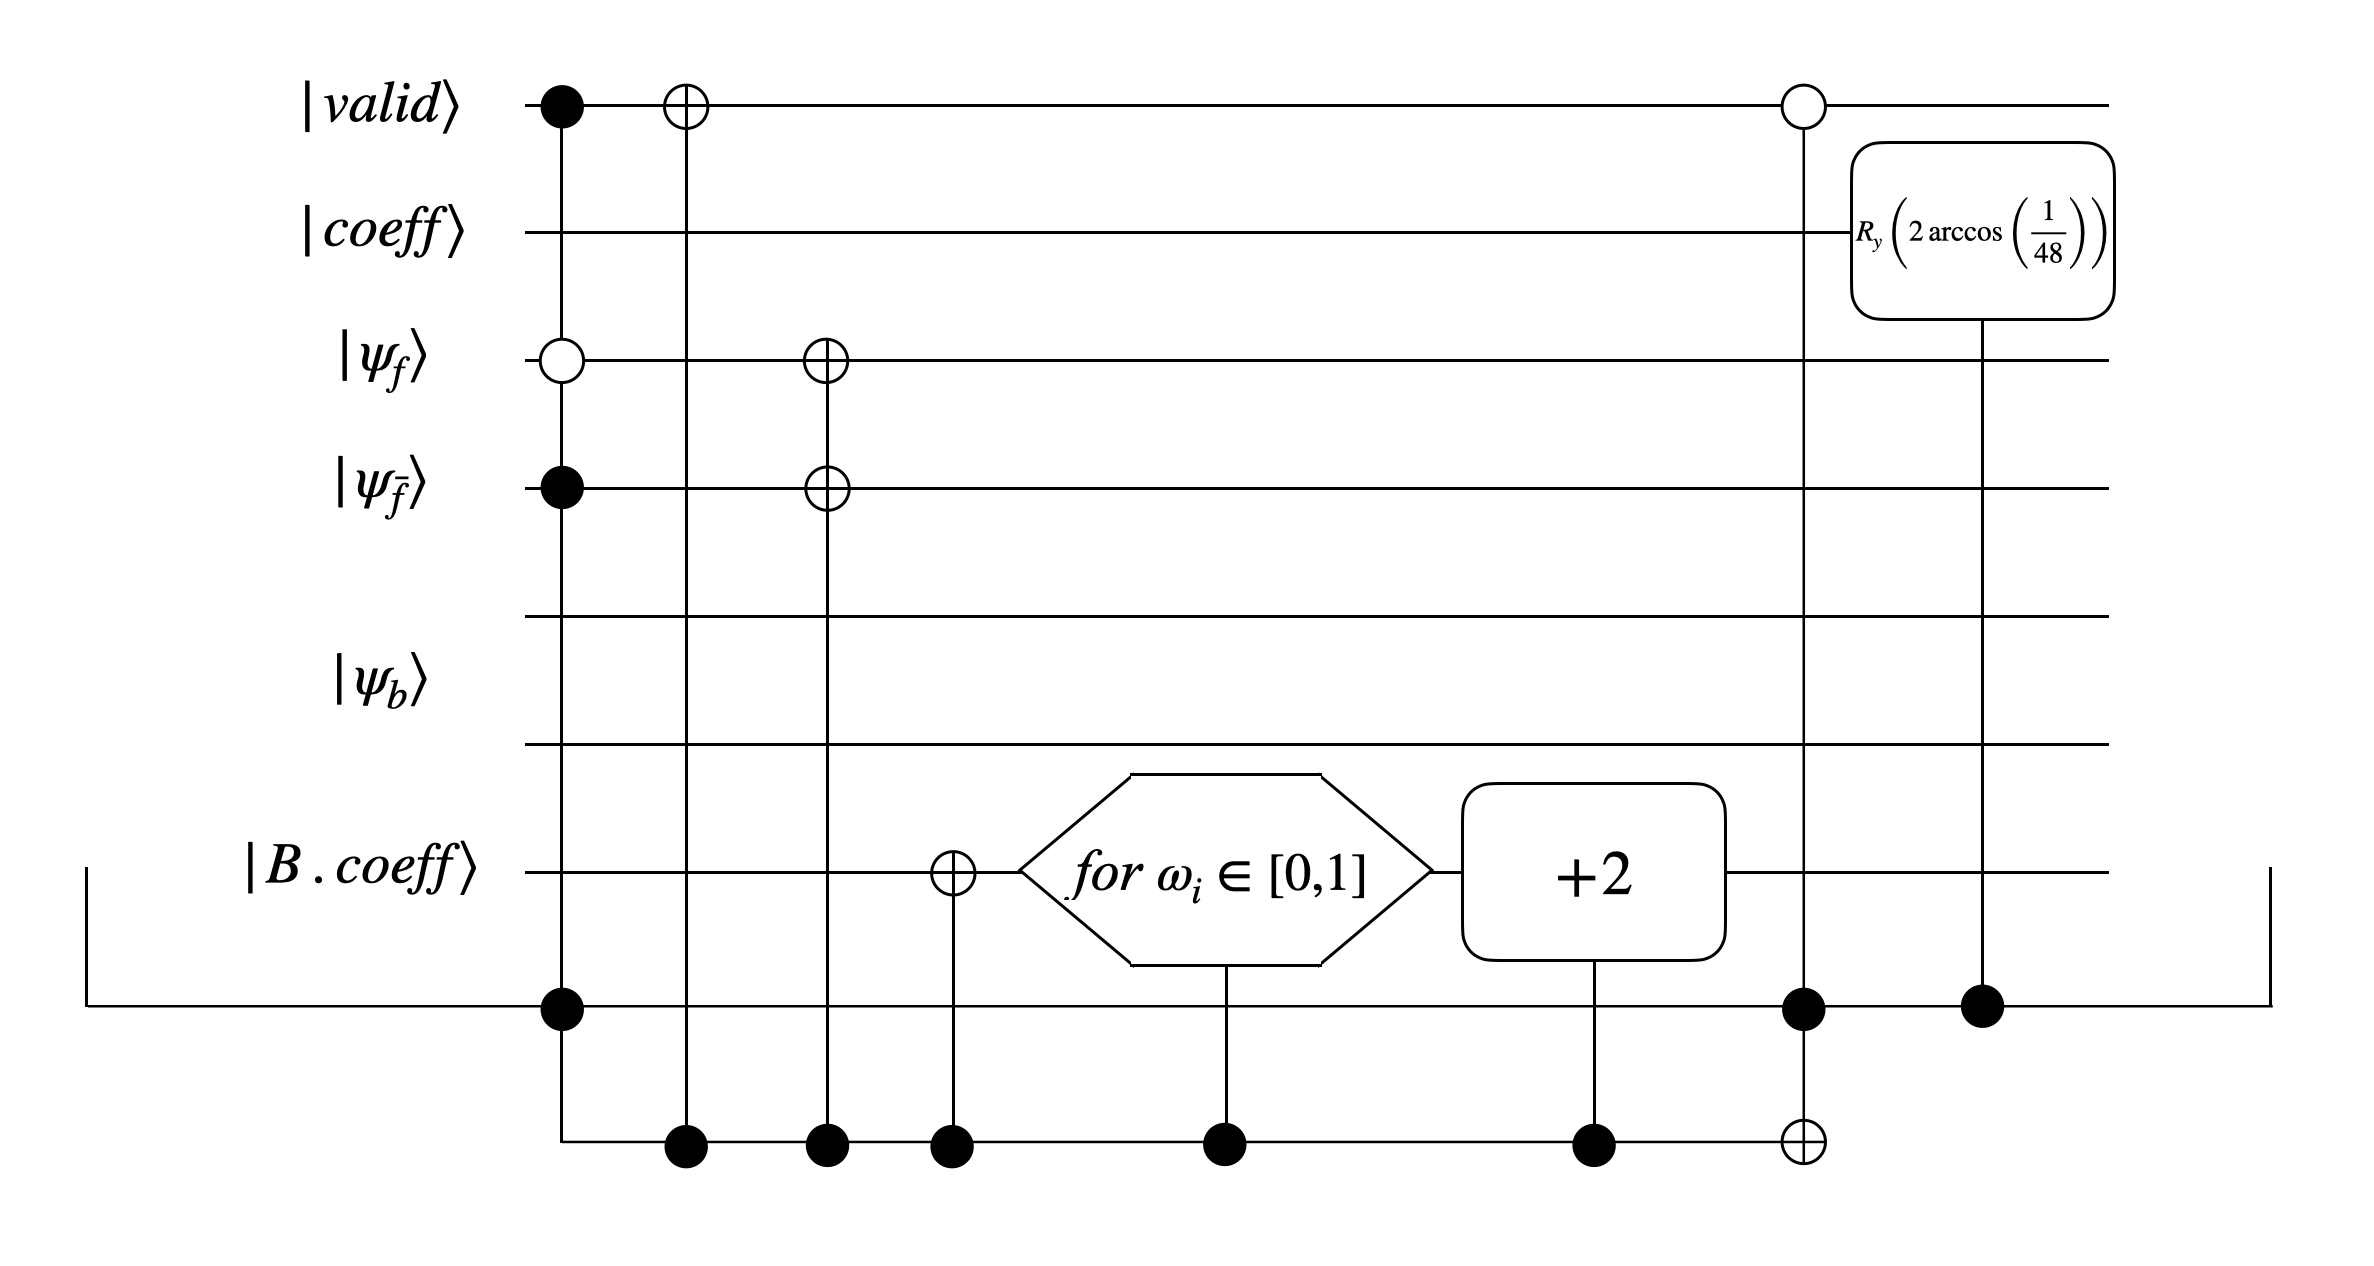
\includegraphics[width = 0.7\linewidth]{figures/T0.png}
    \caption{\textit{Select} unitary $U_{T_0}$ that block-encodes $T_0 = \frac{1}{48}b_0^\dagger d_0(a_0^\dagger)^2$}
\end{figure}
\begin{figure}[h]
    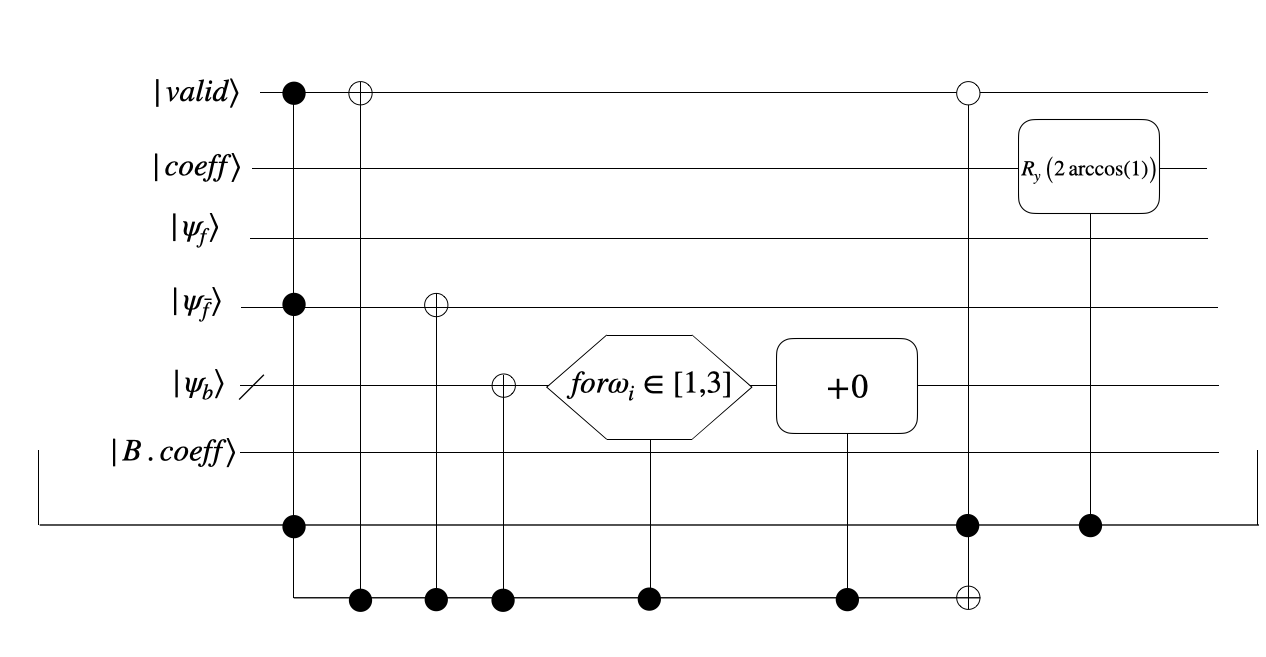
\includegraphics[width = 0.7\linewidth]{figures/T1.png}
    \caption{\textit{Select} unitary $U_{T_1}$ that block-encodes $T_1 = \frac{1}{24}a_0^\dagger a_0 d_0^\dagger$}
\end{figure}
\begin{figure}[h]
    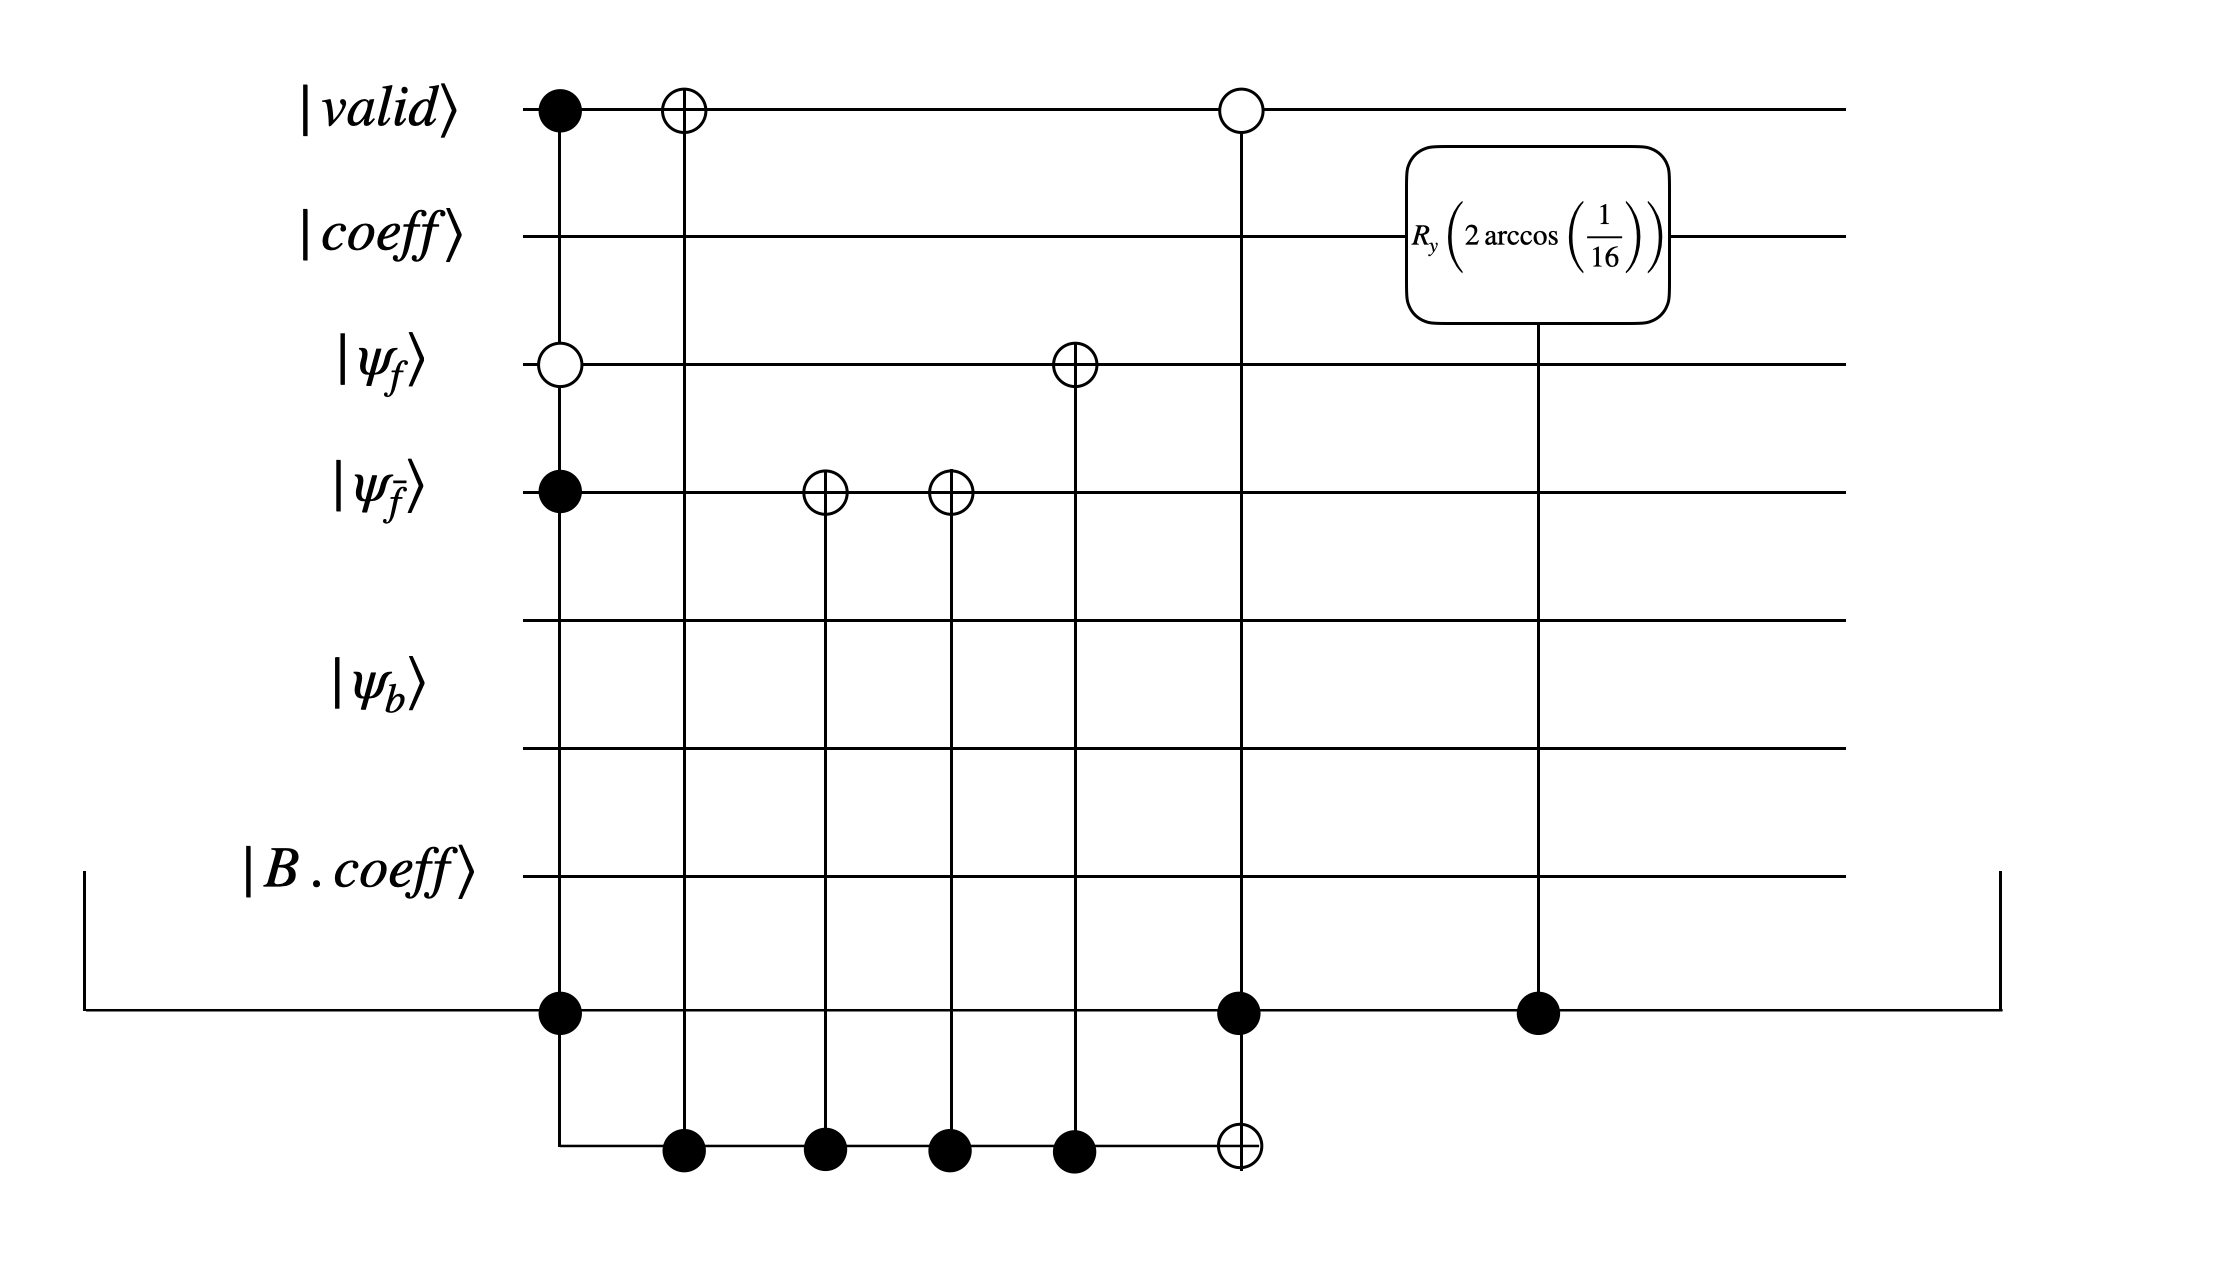
\includegraphics[width = 0.7\linewidth]{figures/T2.png}
    \caption{\textit{Select} unitary $U_{T_2}$ that block-encodes $T_2 = \frac{1}{16}b_0^\dagger d_0^\dagger d_0$}
\end{figure}

\textbf{Step 4: Count gates:} Using the notation in \ref{count gates not.}, the preceeding three unitaries have the following gate counts:

\begin{align}
    C_{U_{T_0}} &= (3, 1, 5, 5)\\
    C_{U_{T_1}} &= (4, 1, 5, 5)\\
    C_{U_{T_2}} &= (1, 1, 3, 3)
\end{align}
Thus, the total cost of the \textit{select} oracle is $C_{\textit{select}} = (8, 3, 13, 13)$. 

\textbf{Step 5: Post-process the eigenvalues:} After obtaining the full block-encoding of the Hamiltonian, the eigenvalues (which can be obtained via phase estimation) must be post-processed. This is because the eigenvalues of the block encoded Hamiltonian will correspond to $\bar{H}$, \textit{not} $H$ (the original problem Hamiltonian).
For this example, $\bar{H} = \frac{1}{48}H$, so if eigenvalues of the block Hamiltonian are obtained as $\bar{E}_i$, then $\bar{E_i} = \frac{1}{48}E_i$. Thus,
\begin{equation}
    E_i = 48\bar{E}_i
\end{equation}
\section{Lightfront Hamiltonians}
\label{subsec:lightfront-hamiltonian}
Here, the explicit discrete form of the Yukawa and $\phi^4$ Hamiltonians will be written out in lightfront coordinates. 

\subsection{Yukawa}
The Hamiltonian is written in terms of fields of discrete momenta, confined to a box, with integration of the Hamiltonian density $\mathcal{H}$ over lightfront space $x^-$:
\begin{align}
    \label{eq:yukawa-hamiltonian-fields}
    H &= H_0 + g\int_{-L}^L dx^- \bar \psi(x) \psi(x) \phi(x)\\ 
    &+ g^2\int_{-L}^L  dx^- \bar \psi(x) \phi(x) \gamma^+\left(i\partial^+ \right)^{-1}\phi(x) \psi(x) \nonumber
\end{align}

The discretized fields are given as:

\begin{align}
    \psi(x) &= \sum_{k = 1/2}^\infty\frac{b_k u(p_k)e^{-ip_k x} + d_k^\dagger v(p_k)e^{ip_k x}}{\sqrt{4\pi k}}\\ 
    \bar \psi(x)&= \sum_{k = 1/2}^\infty\frac{b_k^\dagger \bar u(p_k)e^{ip_k x} + d_k \bar v(p_k)e^{-ip_k x}}{\sqrt{4\pi k}}\\
    \phi(x) &= \sum_{k = 1}^\infty\frac{a_k e^{-ip_k x} + a_k^\dagger e^{ip_k x}}{\sqrt{4\pi k}}
\end{align}

The free part of the Hamiltonian is 

\begin{equation}
    H_0 = \sum_{k = 1/2}^\infty \frac{m_F^2}{p_k^+}\left(b_k^\dagger b_k + d_k^\dagger d_k \right) + \sum_{k = 1}^\infty \frac{m_B^2}{p_k^+}a_k^\dagger a_k 
\end{equation}

Taking a product of the fields and integrating, we get: 
\begin{align*}
    \int_{-L}^L dx^- \bar \psi(x) \psi(x) \phi(x)  = \frac{g(2L)^{5/2}}{(4\pi)^{3/2}} \sum_{k_1, k_2, k_3}^\infty \frac{1}{\sqrt{k_1k_2k_3}}& \left(  b_{k_1}^\dagger b_{k_2}a_{k_3}\bar u(p_{k_1})u(p_{k_2})\delta_{k_1, k_2 + k_3}  \right. \\
      &\left. + b_{k_1}^\dagger b_{k_2}a^\dagger_{k_3}\bar u(p_{k_1})u(p_{k_2})\delta_{k_1 + k_3, k_2} \right)\\
      &\left. + b_{k_1}^\dagger d_{k_2}^\dagger a_{k_3} \bar u(p_{k_1})v(p_{k_2})\delta_{k_1 + k_2, k_3} \right)\\
      &\left. -  b_{k_2}d_{k_1} a^\dagger_{k_3}\bar v(p_{k_1})u(p_{k_2})\delta_{k_3, k_1 + k_2} \right)\\
      &\left. -d_{k_2}^\dagger d_{k_1}  a_{k_3}\bar v(p_{k_1})v(p_{k_2})\delta_{k_2, k_1 + k_3} \right)\\
      &\left. -d_{k_2}^\dagger d_{k_1}  a^\dagger_{k_3}\bar v(p_{k_1})v(p_{k_2})\delta_{k_1, k_2 + k_3} \right)
\end{align*}

where 
\begin{align}
    &\bar u(p_k) u(q_k) = \bar v(p_k) v(q_k) = \sqrt{p_k^+ q_k^+}\left(\frac{m}{p_k^+} + \frac{m}{q_k^+} \right)\\
    &\bar u(p_k) v(q_k) = \bar v(p_k) u(q_k) = \sqrt{p_k^+ q_k^+}\left(\frac{m}{q_k^+} - \frac{m}{p_k^+} \right)
\end{align}

The discretized momentum is given by $p_k = \frac{2\pi k}{L}$

Lastly, the interaction term unique to lightfront coordinates in equation \ref{eq:yukawa-hamiltonian-fields} can be written as:
\begin{align*}
    \int_{-L}^L dx^- \bar \psi(x) \phi(x) \gamma^+ \left(i\partial^+ \right) \phi(x) \psi(x) = \frac{g(2L)^3}{(4\pi)^{2}} \sum_{k_1, k_2, k_3,k_4}^\infty \frac{1}{\sqrt{k_1k_2k_3k_4}}& \left(  b_{k_1}^\dagger b_{k_4}a_{k_2}a_{k_3}\frac{\bar u(p_{k_1})\gamma^+u(p_{k_4})}{p_{k_3} + p_{k_4}}\delta_{k_1, k_2 + k_3 + k_4}  \right. \\
     & \left.-b_{k_1}^\dagger d_{k_4}^\dagger a_{k_2}a_{k_3}\frac{\bar u(p_{k_1})\gamma^+v(p_{k_4})}{p_{k_4} - p_{k_3}}\delta_{k_1 + k_4, k_2 + k_3}\right)  \\
     & \left.-b_{k_1}^\dagger b_{k_4} a_{k_2}a_{k_3}^\dagger \frac{\bar u(p_{k_1})\gamma^+u(p_{k_4})}{p_{k_3} - p_{k_4}}\delta_{k_1 + k_3, k_2 + k_4}\right)  \\
     & \left.-b_{k_1}^\dagger d_{k_4}^\dagger a_{k_2}a_{k_3}^\dagger \frac{\bar u(p_{k_1})\gamma^+v(p_{k_4})}{p_{k_3} + p_{k_4}}\delta_{k_2, k_1 + k_4 + k_3}\right)  \\
     & \left.+b_{k_1}^\dagger b_{k_4} a_{k_2}^\dagger a_{k_3} \frac{\bar u(p_{k_1})\gamma^+u(p_{k_4})}{p_{k_3} + p_{k_4}}\delta_{k_1 + k_2,k_3 + k_4}\right)  \\
     & \left.-b_{k_1}^\dagger d_{k_4}^\dagger a_{k_2}^\dagger a_{k_3} \frac{\bar u(p_{k_1})\gamma^+v(p_{k_4})}{p_{k_4} - p_{k_3}}\delta_{k_3, k_2 + k_1+ k_4}\right)  \\
     & \left.-b_{k_1}^\dagger b_{k_4} a_{k_2}^\dagger a_{k_3}^\dagger \frac{\bar u(p_{k_1})\gamma^+u(p_{k_4})}{p_{k_3} - p_{k_4}}\delta_{k_4, k_2 + k_3 + k_1}\right)  \\
     & \left.+d_{k_4}^\dagger d_{k_1} a_{k_2}a_{k_3} \frac{\bar v(p_{k_1})\gamma^+u(p_{k_4})}{p_{k_4} - p_{k_3}}\delta_{k_4, k_1 + k_2 + k_3}\right)  \\
     & \left. +b_{k_4} d_{k_1} a_{k_2}a_{k_3}^\dagger \frac{\bar v(p_{k_1})\gamma^+v(p_{k_4})}{p_{k_3} - p_{k_4}}\delta_{k_3, k_1 + k_2 + k_4}\right)  \\
     & \left. +d_{k_4}^\dagger d_{k_1} a_{k_2}a_{k_3}^\dagger \frac{\bar v(p_{k_1})\gamma^+u(p_{k_4})}{p_{k_3} + p_{k_4}}\delta_{k_4 + k_3, k_1 + k_2}\right)  \\
     & \left.-b_{k_4} d_{k_1} a_{k_2}^\dagger a_{k_3} \frac{\bar v(p_{k_1})\gamma^+u(p_{k_4})}{p_{k_3} + p_{k_4}}\delta_{k_2, k_4 + k_1 + k_3}\right)  \\
     & \left.+d_{k_4}^\dagger d_{k_1} a_{k_2 }^\dagger a_{k_3}^\dagger \frac{\bar v(p_{k_1})\gamma^+v(p_{k_4})}{p_{k_4} - p_{k_3}}\delta_{k_1, k_2 + k_3 + k_4}\right)  \\
     & \left.-b_{k_4} d_{k_1} a_{k_2}^\dagger a_{k_3}^\dagger \frac{\bar v(p_{k_1})\gamma^+u(p_{k_4})}{p_{k_3} - p_{k_4}}\delta_{k_1 + k_4, k_2 + k_3 }\right)  \\
     & \left.-b_{k_4} d_{k_1} a_{k_2}^\dagger a_{k_3}^\dagger \frac{\bar v(p_{k_1})\gamma^+u(p_{k_4})}{p_{k_3} + p_{k_4}}\delta_{k_1 + k_4, k_2 + k_3}\right)  \\
\end{align*}

where 

\begin{align}
    &\bar u(p_k)\gamma^+ u(q_k) = \bar v(p_k)\gamma^+ v(q_k) = 2\sqrt{p_k^+ q_k^+}\\
    &\bar u(p_k)\gamma^+ v(q_k) = \bar v(p_k)\gamma^+ u(q_k) = -2\sqrt{p_k^+ q_k^+}
\end{align}

\subsection{$\phi^4$}
\gus{Kamil}
\section{Results (Random Operators)}
\label{sec:random-op-results}

In the previous subsections, the costs associated with LOBE are benchmarked for physically relevant models.
In this subsection, we benchmark the same costs for LOBE for randomly generated operators of form of Eq. \ref{eq:lclo}.
\ws{@Gus, we need to describe here how the "random" protocol in OpenParticle works.}

\begin{figure}
    \centering
    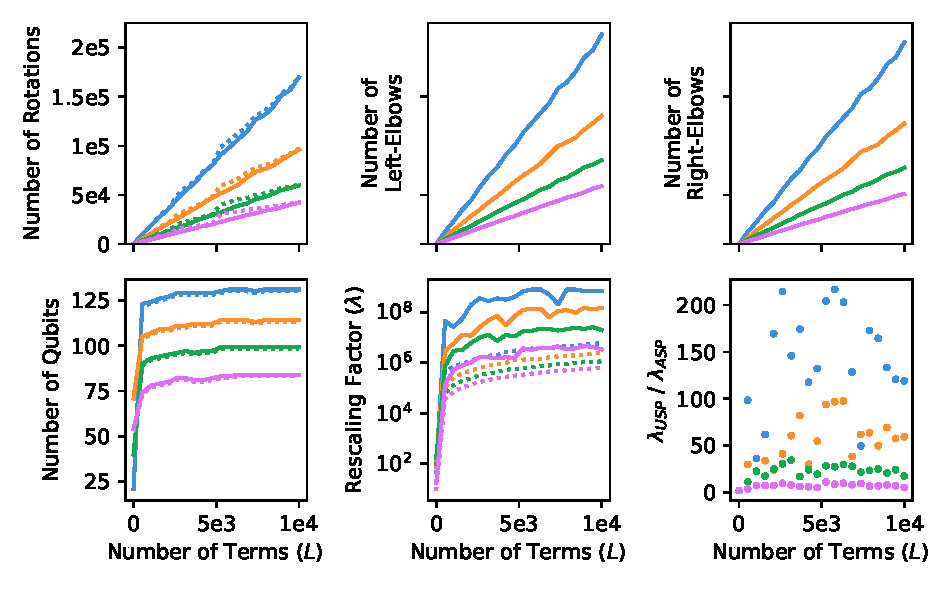
\includegraphics[width=16cm]{figures/random_hamiltonians_metrics_vs_terms.pdf}
    \caption{
        \textbf{Block-Encoding Metrics for Increasing $L$ (Random Hamiltonians).}
        The number of rotations (upper left), left-elbows (upper middle), right-elbows (upper right), number of qubits (lower left), and rescaling factors (lower middle) are plotted as a function of the number of terms in the operator ($L$).
        In the lower right subfigure, the ratio of the two rescaling factors is shown.
        The gate counts for the variant of LOBE using \textit{USP} are shown as the solid lines and those using \textit{ASP} are shown as the dotted lines.
        Metrics for different values of the bosonic occupation cutoff ($\Omega$) are represented in the different colors: $\Omega = 15$ (blue), $\Omega = 7$ (orange), $\Omega = 3$ (green), and $\Omega = 1$ (purple).
        The number of momentum modes ($I$) is set to $15$ and the maximum number of ladder operators per term is set to $5$ ($A_l + B_l + D_l \leq 5$).
        The number of rotations excludes rotations by angles that result in Clifford operations.
    }
    \label{fig:random_hamiltonians_metrics_vs_terms}
\end{figure}

\begin{figure}
    \centering
    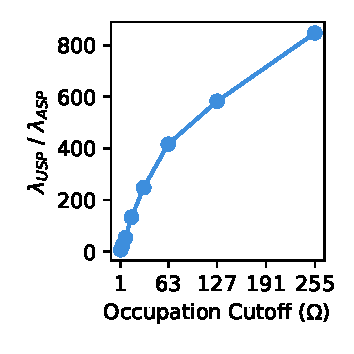
\includegraphics[width=6cm]{figures/random_hamiltonians_rescaling_factor_ratios_vs_omega.pdf}
    \caption{
        \textbf{Ratio of Rescaling Factors for Increasing $\Omega$ (Random Hamiltonians).}
        The average ratio of the two rescaling factors ($\lambda_{USP}$ and $\lambda_{ASP}$) is shown as a function of increasing bosonic occupation cutoff ($\Omega$).
        The number of momentum modes ($I$) is set to $15$ and the maximum number of ladder operators per term ($A + B$) is set to $5$.
        The ratios plotted are the average ratio over 20 unique values of $L$ linearly spaced between $1$ and $10000$.
    }
    \label{fig:random_hamiltonians_rescaling_factor_ratios_vs_omega}
\end{figure}

In Figure \ref{fig:random_hamiltonians_metrics_vs_terms}, we plot the spacetime quantum resources associated with a LOBE block-encoding for randomly generated Hamiltonians.
As is seen for the other models, the number of non-Clifford operations scales linearly with $L$ and the number of qubits scales logarithmically with $L$.
The rescaling factors for both implementations scale logarithmically with $L$.
Additionally, the ratio between the rescaling factors is seemingly independent of $L$, however does appear to increase with $\Omega$.

In Figure \ref{fig:random_hamiltonians_rescaling_factor_ratios_vs_omega}, we plot the average ratio of the rescaling factors for the two variants of LOBE as a function of $\Omega$.
The ratio increases as a function of $\Omega$, indicating that the implementation using \textit{ASP} is increasingly more favorable for models that include a large number of bosons.



\end{document}